\documentclass[11pt]{article}
\usepackage[T1]{fontenc}
\usepackage[utf8]{inputenc}
\usepackage{lmodern}
\usepackage[margin=1.05in]{geometry}
\usepackage{amsmath,amssymb,amsthm,mathtools,bm}
\usepackage{microtype,enumitem,booktabs,longtable,array,etoolbox,needspace}
\usepackage{graphicx,xcolor,tikz}
\usetikzlibrary{arrows.meta,positioning,calc,patterns,decorations.pathreplacing}
\usepackage[numbers,sort&compress]{natbib}
\usepackage[hidelinks,unicode]{hyperref}
\usepackage{bookmark}
\pdfglyphtounicode{parenleftbig}{0028 FE01}
\pdfglyphtounicode{parenrightbig}{0029 FE01}
\pdfglyphtounicode{bracketleftbig}{005B FE01}
\pdfglyphtounicode{bracketrightbig}{005D FE01}
\pdfglyphtounicode{vextendsingle}{20D3}
\pdfglyphtounicode{parenleftBig}{0028 FE02}
\pdfglyphtounicode{parenrightBig}{0029 FE02}
\pdfglyphtounicode{parenleftbigg}{0028 FE03}
\pdfglyphtounicode{parenrightbigg}{0029 FE03}
\pdfglyphtounicode{bracketleftbigg}{005B FE03}
\pdfglyphtounicode{bracketrightbigg}{005D FE03}
\pdfglyphtounicode{floorleftbigg}{230A FE03}
\pdfglyphtounicode{floorrightbigg}{230B FE03}
\pdfglyphtounicode{braceleftbigg}{007B FE03}
\pdfglyphtounicode{bracerightbigg}{007D FE03}
\pdfglyphtounicode{parenleftBigg}{0028 FE04}
\pdfglyphtounicode{parenrightBigg}{0029 FE04}
\pdfglyphtounicode{bracketleftBigg}{005B FE04}
\pdfglyphtounicode{bracketrightBigg}{005D FE04}
\pdfglyphtounicode{braceleftBigg}{007B FE04}
\pdfglyphtounicode{bracerightBigg}{007D FE04}
\pdfglyphtounicode{summationtext}{2211 FE01}
\pdfglyphtounicode{producttext}{220F FE01}
\pdfglyphtounicode{integraltext}{222B FE01}
\pdfglyphtounicode{uniontext}{22C3 FE01}
\pdfglyphtounicode{summationdisplay}{2211 FE02}
\pdfglyphtounicode{productdisplay}{220F FE02}
\pdfglyphtounicode{integraldisplay}{222B FE02}
\pdfglyphtounicode{hatwide}{02C6 FE01}
\pdfglyphtounicode{tildewide}{02DC FE01}
\pdfglyphtounicode{bracketleftBig}{005B FE02}
\pdfglyphtounicode{bracketrightBig}{005D FE02}
\pdfglyphtounicode{radicalbig}{221A FE01}
\pdfglyphtounicode{radicalBig}{221A FE02}
\pdfglyphtounicode{mapsto}{007C}
\pdfgentounicode=1

\numberwithin{equation}{section}
\newtheorem{theorem}{Theorem}[section]
\newtheorem{proposition}[theorem]{Proposition}
\newtheorem{lemma}[theorem]{Lemma}
\newtheorem{corollary}[theorem]{Corollary}
\newtheorem{claim}[theorem]{Claim}
\theoremstyle{definition}
\newtheorem{definition}[theorem]{Definition}
\theoremstyle{remark}
\newtheorem{remark}[theorem]{Remark}
\newcommand{\R}{\mathbb R}
\newcommand{\C}{\mathbb C}
\newcommand{\Z}{\mathbb Z}
\newcommand{\N}{\mathbb N}
\newcommand{\Q}{\mathbb Q}
\newcommand{\E}{\mathbb E}
\newcommand{\Prob}{\mathbb P}
\newcommand{\widehatC}{\widehat{\mathbb C}}
\newcommand{\eps}{\varepsilon}
\newcommand{\dd}{\,\mathrm d}
\newcommand{\ind}{\mathbf 1}
\newcommand{\one}{\mathbf 1}
\newcommand{\law}{\operatorname{Law}}
\newcommand{\supp}{\operatorname{supp}}
\newcommand{\diam}{\operatorname{diam}}
\newcommand{\dist}{\operatorname{dist}}
\newcommand{\Leb}{\operatorname{Leb}}
\newcommand{\Var}{\operatorname{Var}}
\newcommand{\Cov}{\operatorname{Cov}}
\newcommand{\id}{\operatorname{id}}
\newcommand{\sgn}{\operatorname{sgn}}
\newcommand{\rank}{\operatorname{rank}}
\newcommand{\tr}{\operatorname{tr}}
\newcommand{\EL}{\operatorname{EL}}
\newcommand{\CLE}{\mathrm{CLE}}
\newcommand{\SLE}{\mathrm{SLE}}
\newcommand{\LQG}{\mathrm{LQG}}
\newcommand{\GFF}{\mathrm{GFF}}
\newcommand{\FK}{\mathrm{FK}}
\newcommand{\PV}{\operatorname{PV}}
\newcommand{\cB}{\mathcal B}
\newcommand{\cF}{\mathcal F}
\newcommand{\cG}{\mathcal G}
\newcommand{\cK}{\mathcal K}
\newcommand{\cT}{\mathcal T}
\newcommand{\cU}{\mathcal U}
\newcommand{\cV}{\mathcal V}
\newcommand{\cW}{\mathcal W}
\newcommand{\cL}{\mathcal L}
\newcommand{\cH}{\mathcal H}
\newcommand{\cA}{\mathcal A}
\newcommand{\cD}{\mathcal D}
\newcommand{\cM}{\mathcal M}
\newcommand{\cP}{\mathcal P}
\newcommand{\cS}{\mathcal S}
\newcommand{\cI}{\mathcal I}
\newcommand{\cJ}{\mathcal J}
\BeforeBeginEnvironment{proof}{\Needspace{5\baselineskip}}
\newcommand{\proofstage}[1]{\par\Needspace{4\baselineskip}\smallskip
  \noindent\textit{#1.}\par\nopagebreak\smallskip\nopagebreak}
\setlist{itemsep=3pt,topsep=5pt}
\setlength{\emergencystretch}{2em}
\hypersetup{pdftitle={The critical Liouville quantum sphere and geometric limits of FK maps at q=4},pdfauthor={OpenAI}}

\title{The critical Liouville quantum sphere and\\geometric limits of FK maps at $q=4$}
\author{OpenAI}
\date{September 24, 2026}
\begin{document}
\maketitle
\begin{abstract}
We construct the field and area law of the unit-area critical Liouville
quantum sphere as a limit of ordinary subcritical quantum spheres, and
equip it with its critical intrinsic metric. We then prove that spherical
Fortuin--Kasteleyn planar maps at $q=4$, embedded by their equilateral flag
uniformizations, converge jointly to this sphere decorated by an independent
nested conformal loop ensemble $\CLE_4$. With deterministic distance
normalization, the convergence includes the area measure, the full embedded
distance function, and every macroscopic interface through all positive
integer edge counts.
\end{abstract}

\section{Introduction and statements}\label{sec:intro}

Random planar maps provide discrete models of random two-dimensional geometry. Decorating a map by a critical Fortuin--Kasteleyn random-cluster configuration \cite{FortuinKasteleyn1972} couples that geometry to a loop ensemble. The expected continuum objects are Liouville quantum gravity surfaces decorated by conformal loop ensembles. The endpoint $q=4$ is distinguished by critical quantum gravity and logarithmic corrections in the discrete encoding.

Sheffield's inventory model established a correspondence between decorated
planar maps and two-type inventory trajectories, and identified the transition
at $q=4$ \cite{SheffieldInventory}.  Duplantier, Miller, and Sheffield
constructed subcritical quantum surfaces by mating continuum trees
\cite{DMS}.  At the critical endpoint, Aru, Holden, Powell, and Sun established
the Brownian half-plane-excursion coupling for quantum disks and the
near-critical convergence of their fields and quantum measures
\cite{AHPScritical}.  The limiting Brownian data do not by themselves determine
the decorated critical surface.  Da Silva, Hu, Powell, and Wong proved the
critical infinite-volume FK encoding limit with its logarithmic discrepancy normalization and
an exact fully packed loop description \cite{DSHPW}.  Our geometric theorem
retains the actual conformal structure, the original graph metric, area, and
all macroscopic interfaces in one finite-map limit.

The area construction builds on critical Gaussian multiplicative chaos.
Duplantier--Rhodes--Sheffield--Vargas constructed the derivative chaos and
identified its relation to Seneta--Heyde normalization
\cite{DRSVderivative,DRSV}.  Powell proved universality of derivative-normalized
convolution approximations under stated mollifier hypotheses \cite{Powell};
the circle-average Seneta--Heyde construction is treated by
Huang--Rhodes--Vargas \cite[Theorem~4.2]{HRVcriticalDisk}.
Aru--Powell--Sep\'ulveda proved the fixed-field limit
$(2-\gamma)^{-1}\mu^\gamma\to2\mu'$ \cite[Theorem~1.1]{APS}.
Section~\ref{sec:continuum} specializes the corrected cutoff argument to
circle averages and passes to the varying, area-normalized sphere law.
Its starting law is the ordinary subcritical sphere of
\cite[Definition~4.21(ii) and Proposition~A.13]{DMS}.

For $0<\gamma<2$, Aru--Huang--Sun identify the DMS unit-area sphere
with three independent area marks with the unit-volume sphere of
David--Kupiainen--Rhodes--Vargas with three insertions of weight $\gamma$
\cite[Theorem~1.1]{AHSSphereEquivalence}.
The latter authors also discuss sphere constructions at
$\gamma=2$ \cite[Section~4.1]{DKRVSphere}.
Here we study the critical limit of the ordinary DMS area-one law,
retaining the area-sampling interpretation of its marks.

The metric construction uses the critical local metric and Euclidean topology
of Ding--Gwynne \cite{DGuniqueness,DGtopology}.  We prove the additional
critical coordinate-change and sphere-completion statements in
Section~\ref{sec:continuum}; the coordinate argument follows the
local linearization and annular comparison strategy of Gwynne--Miller
\cite[Sections~2--3]{GMCovariance}, using the Euclidean-topology estimates
available at criticality.  The later rigidity argument adapts Ding--Gwynne's
optimal-comparison and field-perturbation strategy to discrete passage
profiles, for which the required conditional laws must first be established.
Field reconstruction uses the log-mass strategy of
Berestycki--Sheffield--Sun and the critical reconstruction framework of Vihko
\cite{BSSReconstruction,VihkoReconstruction}, with the local normalization and
comparison-class argument given in Section~\ref{sec:conformal}.

Quantum-disk exploration provides a separate source of geometric information.
Miller--Sheffield--Werner established the subcritical simple-CLE disk cutting
laws \cite{MSWQuantum}, while Kammerer identified the critical total-perimeter
process and related exploration distances \cite{Kammerer}.
Ang--Gwynne proved the conditional independent-disk law for components of an
independent $\CLE_4$ on a critical disk and identified their boundary lengths
through a reweighted $3/2$-stable process
\cite[Theorems~1.1--1.2]{AngGwynneCritical}.
We retain these antecedents while proving the marked two-side cutting law,
exact attachment rules, and finite-map comparisons needed here.
The conformal loop and field inputs come from the loop-soup construction and
sphere nesting \cite{SWcle,KWnested}, the GFF contour coupling
\cite{SchrammSheffieldContour}, and the subsequent signed exploration,
level-line, and bounded-type local-set theories
\cite{MSWTrunk,WangWu,ASWlocal,ASlocal}.

The two main conclusions are the independently specified critical sphere of
Theorem~\ref{thm:continuum} and the joint finite-map limit of
Theorem~\ref{thm:main}. The passage from the FK encoding to this geometric
limit has three distinct stages. Exact contacts and incidence comparisons
first identify the entire flag sphere up to a homeomorphism. Conditional
laws for local observations then identify its prescribed conformal
uniformization and compare its graph distances with the critical metric.
Finally, an estimate controlling every vertex extends the local distance
comparison to the full embedded distance function. Each stage is proved
at $q=4$; no convergence theorem for FK maps at another value of $q$ is used.

\subsection{The finite model and its canonical embedding}

Let $\mathcal F_n$ be the set of pairs $(M,A)$ in which $M$ is a rooted connected planar multigraph with $n$ edges in the oriented sphere and $A\subseteq E(M)$. Maps are considered up to orientation-preserving homeomorphism preserving the distinguished oriented root edge and $A$. Loops and multiple edges are allowed. The spanning subgraph $(V(M),A)$ includes its isolated vertices. If $M^*$ is the dual map, let $A^*$ consist of the dual edges crossing $E(M)\setminus A$. Write $k$ for the number of components and set
\begin{equation}\label{intro:fk-weight}
 \ell(M,A)=k(A)+k(A^*)-1
 =2k(A)+|A|-|V(M)|,
 \qquad
 \Prob\{(M_n,A_n)=(M,A)\}
 =\frac{2^{\ell(M,A)}}{Z_n(4)}.
\end{equation}
Here $Z_n(4)$ is the sum of the displayed weights over $\mathcal F_n$. In particular, the factor depending on $|V(M)|$ is part of the law. Let $d_n$ be shortest-path distance on the original primal vertices, using every original edge with length one.

For each endpoint-and-side incidence occurrence of an original edge, take an equilateral Euclidean triangle with corners labelled $v,e,f$: the original vertex, the edge midpoint, and the face center. Repeated occurrences at loops or bridges remain distinct. Glue the $4n$ triangles according to their incidence identifications. The resulting oriented polyhedral sphere $X_n$ has its conformal structure extended across its conical vertices. Let $m_n$ be normalized Euclidean area, giving mass $1/(4n)$ to each triangle.

Conditionally on $X_n$, sample $x_n^1,x_n^2,x_n^3$ independently from $m_n$. Almost surely they are distinct. Let
\[
 \phi_n:X_n\longrightarrow\widehatC,
 \qquad \phi_n(x_n^1)=0,\quad
 \phi_n(x_n^2)=1,\quad \phi_n(x_n^3)=\infty,
\]
be the unique orientation-preserving conformal uniformization
\cite[Theorem~II.2.15]{SaintGervaisUniformization}. This prescription is part of the discrete model. Let $\rho$ denote the standard spherical distance on $\widehatC$.

We also fix the interface drawing. In a flag triangle retain the closed region whose barycentric coordinate at $v$ is at least $2/3$. If its original edge belongs to $A_n$, retain in addition the region whose barycentric coordinate at $f$ is at most $1/3$. Glue these regions with the flags. Their polygonal boundary components are the FK interfaces. Let $\Gamma_n$ be their images under $\phi_n$, as unrooted, unoriented loops, retaining every nesting level and every occurrence. Figure~\ref{fig:flags} depicts the local prescription. The flag geometry defines the conformal structure and drawing; $d_n$ is the original primal graph distance.

\begin{figure}[htbp]
\centering
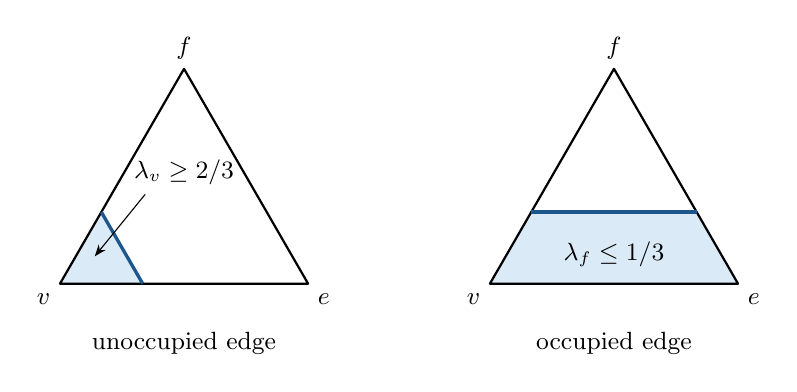
\begin{tikzpicture}[scale=1.05,line join=round,font=\small]
\definecolor{flagblue}{RGB}{28,86,141}
\definecolor{flagfill}{RGB}{218,234,247}
\begin{scope}
\coordinate (v) at (0,0);\coordinate (e) at (3,0);\coordinate (f) at (1.5,2.598);
\fill[flagfill] (v)--(1,0)--(.5,.866)--cycle;
\draw[thick] (v)--(e)--(f)--cycle;
\draw[flagblue,very thick] (1,0)--(.5,.866);
\node[below left] at (v) {$v$};\node[below right] at (e) {$e$};\node[above] at (f) {$f$};
\node[below=14pt] at (1.5,0) {unoccupied edge};
\node at (1.5,1.35) {$\lambda_v\geq2/3$};
\draw[-{Stealth[length=1.5mm]},thin] (1.03,1.08)--(.42,.33);
\end{scope}
\begin{scope}[xshift=5.2cm]
\coordinate (v2) at (0,0);\coordinate (e2) at (3,0);\coordinate (f2) at (1.5,2.598);
\fill[flagfill] (0,0)--(3,0)--(2.5,.866)--(.5,.866)--cycle;
\draw[thick] (v2)--(e2)--(f2)--cycle;
\draw[flagblue,very thick] (.5,.866)--(2.5,.866);
\node[below left] at (v2) {$v$};\node[below right] at (e2) {$e$};\node[above] at (f2) {$f$};
\node[below=14pt] at (1.5,0) {occupied edge};
\node at (1.5,.36) {$\lambda_f\leq1/3$};
\end{scope}
\end{tikzpicture}

\caption{The retained region in one equilateral flag. The left panel applies when the original edge is unoccupied; the right panel adds the strip next to $ve$ when it is occupied. The blue segments inside a flag are interface pieces; sides shared with adjacent flags are glued before the boundary is taken. Labels specify incidence occurrences, so the same construction applies to loops and bridges.}
\label{fig:flags}
\end{figure}

The embedded distance graph at scale $a>0$ is the compact set
\begin{equation}\label{intro:distance-graph}
 K_n(a)=\{(\phi_n(u),\phi_n(v),a d_n(u,v)):
                  u,v\in V(M_n)\}.
\end{equation}

\subsection{The independently specified continuum law}

For $\sqrt2<\gamma<2$, take the ordinary unit-area $\gamma$-quantum sphere of \cite[Definition~4.21(ii)]{DMS}, disintegrated at area one, with its original marked points forgotten. Sample three independent points from its area measure, and use the orientation-preserving coordinate sending them to $0,1,\infty$. Write $h_\gamma$ for the field in that coordinate. We use the circle-average convention
\[
 \mu_h^\gamma(\dd z)
  =\lim_{\eps\downarrow0}
       \eps^{\gamma^2/2}e^{\gamma h_\eps(z)}\,\dd^2z.
\]
Define
\begin{align}
 Q_\gamma&=\frac2\gamma+\frac\gamma2,
 &c_\gamma&=\frac1\gamma\log\bigl(2(2-\gamma)\bigr),
 &\widehat h_\gamma&=h_\gamma+c_\gamma,\label{intro:renormalization}\\
 \nu_\gamma&=\frac{\mu_{\widehat h_\gamma}^\gamma}{2(2-\gamma)}
             =\mu_{h_\gamma}^\gamma,
 &H_\gamma&=\widehat h_\gamma-
                \frac{Q_\gamma}{2}\log g_{\rm round},
 &g_{\rm round}(z)&=\frac4{(1+|z|^2)^2}.
 \label{intro:round-field}
\end{align}
The expression in the chart at infinity agrees, so $H_\gamma$ is a scalar distribution on the round sphere. The factor in \eqref{intro:renormalization} is fixed by the local normalization
$\mu^\gamma/[2(2-\gamma)]\to\mu^{\rm crit}$ for a fixed ordinary GFF \cite{APS}; the convergence of the varying marked sphere laws is part of the following theorem.

\begin{theorem}[The critical area-marked sphere]\label{thm:continuum}
As $\gamma\uparrow2$, the laws of $(H_\gamma,\nu_\gamma)$ converge to a unique nondegenerate probability law $\mathsf P_{\rm crit}$ in
\[
 H^{-1}(S^2,g_{\rm round})\times\mathcal P(S^2),
\]
with the norm topology in the first factor and the weak topology in the second. Let $(H,\nu)$ have this law and set $h=H+\log g_{\rm round}$ in local conformal coordinates. Then $\nu=\mu_h^{\rm crit}$, where on compact sets avoiding $0,1,\infty$,
\begin{equation}\label{intro:critical-area}
 \mu_h^{\rm crit}(\dd z)
 =\lim_{\eps\downarrow0}
  \bigl(2\log(1/\eps)-h_\eps(z)\bigr)
        \eps^2e^{2h_\eps(z)}\,\dd^2z
\end{equation}
locally weakly in probability. This positive measure extends across the three marks without atoms, has full support, and has total mass one.

After forgetting the three marks, sampling three new conditionally independent area points and normalizing them to $0,1,\infty$ recovers $\mathsf P_{\rm crit}$. If $f$ maps the new coordinate to the old one, the field transforms as
\[
 h_{\rm new}=h_{\rm old}\circ f+2\log|f'|.
\]

With any one fixed deterministic normalization of the Ding--Gwynne critical local metric, the compatible chart metrics define an intrinsic length metric on the sphere punctured at the three marks. Its completion adds exactly those marks and is a finite continuous metric $D_h$ on $S^2$, inducing the usual topology. The area and completed metric are measurable functions of the same field and obey the corresponding charge-$2$ coordinate rules.
\end{theorem}

Conditionally on $(H,\nu)$, let $\Gamma$ have the M\"obius-invariant whole-plane nested $\CLE_4$ law on the sphere \cite{KWnested}, independently of the entire marked surface. This fixes the decorated continuum target. No convergence of subcritical metrics as $\gamma\uparrow2$ is part of Theorem~\ref{thm:continuum} or needed in its proof.

\subsection{Joint convergence}

We first specify the loop topology. For continuous loops $\eta,\eta':S^1\to S^2$, let $d_{\rm loop}(\eta,\eta')$ be the infimum of their uniform spherical distance over circular orientation-preserving reparametrizations and reversal. Identify representatives at zero distance. A loop collection is locally finite if it contains only finitely many loops of diameter above any positive threshold. An $\eps$-matching of two such collections is a partial bijection that covers every loop of diameter greater than $\eps$ on each side, matches loops at $d_{\rm loop}$-distance at most $\eps$, and leaves only loops of diameter at most $\eps$ unmatched. Loop convergence means the existence of such matchings with $\eps\to0$.

For compact subsets of $S^2\times S^2\times[0,\infty)$, use Hausdorff distance for the product metric
\[
 \rho(z,z')+\rho(w,w')+|r-r'|.
\]

\begin{theorem}[Joint critical universality]\label{thm:main}
For the finite law \eqref{intro:fk-weight}, there is a deterministic sequence $a_n>0$, with $a_n\to0$, such that through all positive integers $n$,
\begin{equation}\label{intro:joint-limit}
 \bigl((\phi_n)_*m_n,K_n(a_n),\Gamma_n\bigr)
 \ \xrightarrow{\ d\ }\
 \bigl(\mu_h^{\rm crit},
       \{(z,w,D_h(z,w)):z,w\in S^2\},\Gamma\bigr).
\end{equation}
Here $(H,\mu_h^{\rm crit})\sim\mathsf P_{\rm crit}$, the area topology is weak convergence, the distance-graph topology is the Hausdorff topology just defined, and the loop topology is convergence by $\eps$-matchings. All nesting and multiplicities are retained. In the same joint convergence,
\begin{equation}\label{intro:flag-mesh}
 \max_{T\ \text{flag of }X_n}\diam_\rho\phi_n(T)
       \ \xrightarrow{\ \Prob\ }0.
\end{equation}
The metric normalization is the one fixed in Theorem~\ref{thm:continuum}; changing it by a deterministic factor changes $a_n$ by that factor.
\end{theorem}

The Hausdorff assertion in \eqref{intro:joint-limit} controls every approaching pair of vertices. It therefore includes possible exceptional endpoints and does not require selecting a finite set of typical vertices. The theorem makes no claim of an explicit power law for $a_n$, a convergence rate, or a formula for the critical metric dimension.

Forgetting the embedding gives the following metric-measure consequence.
For a loop edge, each of its two endpoint occurrences contributes one to
the degree.

\begin{corollary}[The compact metric-measure limit]\label{intro:ghp}
Define a probability measure on the primal vertices by
\[
 \eta_n=\sum_{v\in V(M_n)}\frac{\deg_{M_n}(v)}{2n}\,\delta_v.
\]
With the deterministic normalization of Theorem~\ref{thm:main},
\[
 (V(M_n),a_nd_n,\eta_n)
 \ \xrightarrow{\ d\ }\
 (S^2,D_h,\mu_h^{\rm crit})
\]
in the Gromov--Hausdorff--Prokhorov topology, jointly with the embedded
area and loop convergence in that theorem.
\end{corollary}

\begin{proof}
This is a deterministic consequence of the distance-graph and flag-mesh
assertions of Theorem~\ref{thm:main}. Work on a representation on which
those assertions and the weak area convergence hold almost surely.
Every endpoint occurrence has two side flags, so sending each flag to
its primal vertex pushes $m_n$ to $\eta_n$, including at loops and
bridges. The spherical displacement of this projection is at most the
maximal flag mesh. Consequently
$\widetilde\eta_n=(\phi_n)_*\eta_n$ converges weakly to
$\mu_h^{\rm crit}$, and the embedded vertices become dense in $S^2$.

Continuity of $D_h$ and Hausdorff convergence of the full distance graphs
give
\[
 \sup_{u,v\in V(M_n)}
 \bigl|a_nd_n(u,v)-D_h(\phi_n(u),\phi_n(v))\bigr|
 \longrightarrow0.
\]
Indeed, a sequence violating this assertion has a convergent graph-point
subsequence, whose limit belongs to the graph of $D_h$.
Choose $r_n\downarrow0$ large enough to cover the maximal flag mesh and
to couple $\widetilde\eta_n$ with $\mu_h^{\rm crit}$ so that all but
$r_n$ of the mass has spherical displacement at most $r_n$. The relation
$\{(v,z):\rho(\phi_n(v),z)\le r_n\}$ covers both spaces. Its distortion
for $a_nd_n$ and $D_h$ tends to zero by the displayed bound and uniform
continuity of $D_h$, and it carries all but $r_n$ of the lifted coupling.
The correspondence-and-coupling characterization of
Gromov--Hausdorff--Prokhorov convergence proves the assertion. The same
construction on each coupled subsequence proves the stated joint
convergence in law.
\end{proof}

\begin{table}[htbp]
\centering\small
\begin{tabular}{@{}p{0.30\textwidth}p{0.65\textwidth}@{}}
\toprule
Quantity & Convention \\
\midrule
Model parameter & $q=4$ throughout the map theorem; critical LQG parameter $\gamma=2$. \\[3pt]
Discrete size and area & $n$ original edges, $2n$ Tutte triangles, $4n$ flags; each flag has mass $1/(4n)$. \\[3pt]
Graph metric & Every original primal edge has length one; the deterministic unit is $a_n$. \\[3pt]
Perimeter-count unit & $B_n=(2/\pi)\sqrt n\log n$, distinct from the graph-distance unit. \\[3pt]
Critical bulk area & Derivative normalization in \eqref{intro:critical-area}; near-critical divisor $2(2-\gamma)$. \\[3pt]
Conformal normalization & Three independent area samples, sent in order to $0,1,\infty$. \\
\bottomrule
\end{tabular}
\caption{Normalizations retained in both main theorems.  Boundary-length units for auxiliary disks are fixed separately in Section~\ref{sec:proxy}.}
\label{tab:normalizations}
\end{table}

\subsection{Proof structure and reusable arguments}

\paragraph{The target surface and its metric.}
Section~\ref{sec:continuum} proves Theorem~\ref{thm:continuum}
independently of the finite maps. A maximum-centered cylinder
representation exposes the area-conditioning tilt. Uniform tail estimates
permit passage to criticality, and local absolute continuity separates the
observed field from its area marks when the coordinates change. The metric
is then constructed directly from critical local metrics: annular
comparisons prove conformal covariance, and resampling the three marks
completes the metric at the original marks. The field limit and the metric
construction are separate arguments.

\paragraph{The topological comparison.}
Sections~\ref{sec:discrete}--\ref{sec:cutting} retain the exact finite
weight and its perimeter and volume units. A strictly subcritical boundary
proxy controls the images of small quantum arcs and children in the
critical limit. The resulting contact rule specifies exactly which
boundary occurrences represent the same point. Together with discrete
incidence estimates, it yields homeomorphisms comparing the entire flag
sphere, complete loop tours, and area. A loop-counting Palm identity and
unexamined volume reservoirs identify the ordinary area-one sphere law
after conditioning on the exact finite size. At this stage the
homeomorphisms provide topological coordinates; Section~\ref{sec:conformal}
will identify the prescribed flag uniformizations.

\paragraph{Conditional laws for local observations.}
Sections~\ref{sec:walls} and~\ref{sec:kernels} supply the common input
to the conformal and metric arguments. Auxiliary GFF level lines control
the possible local exploration orders when the exterior changes. Integer
gluing constraints, including their residues, describe which raw map
blocks can be assembled. An independent reference experiment is changed
by a density depending on the chart's macroscopic parameters, increment
paths, and exterior discrepancy variables. Once these data are fixed,
the density does not depend on the retained local payloads, which can
therefore be disintegrated over their actual continuation trees. This gives product
conditional laws for buffered observations even after the entire primary
tree is known. One finite choice then describes the whole countable vector
of observation kernels, including all later cost units. These exact
conditional laws make it possible to test many local candidates and to
compare them after a change of the field outside the observed patch.

\paragraph{The actual conformal coordinates.}
Section~\ref{sec:conformal} applies those laws to extremal length on the
flag surface. A transverse-flow argument prevents conformal collapse and
gives a quasiconformal limiting chart. Local determination makes its
distortion tensor deterministic, and the behavior under coordinate
rotations makes that tensor scalar. The three-point normalization therefore
identifies the limiting conformal map. Field reconstruction and elimination
of auxiliary exploration sources put the subsequent comparisons in the
law of the intended pair of fields.

\paragraph{Metric comparison on ordinary patches.}
Section~\ref{sec:metric} compares primal path costs directly with the
critical reference metric. If the optimal lower and upper comparison
factors differed, a fixed local field perturbation would create enough
strict shortcuts to contradict a nearly optimal path. The factors
therefore agree. This also supplies deterministic scale bounds. The
comparison at this point uses paths with open endpoint regions; it does
not yet attach every discrete vertex to its limiting point.

\paragraph{Every endpoint and one deterministic unit.}
Section~\ref{sec:endpoints} reduces that remaining attachment problem
to a bound on bad grid times in balanced peeling segments. Complete
incidence records ensure that a separating path found in an ordinary
local experiment remains valid in every compatible filling of the
unobserved map. Section~\ref{sec:address} counts the possible bad addresses
and combines equality constraints with survival estimates to prove the
required bound. The resulting uniform endpoint modulus identifies the
entire compact distance graph. Finally,
a bounded monotone calibration removes the deterministic scalar on every
subsequence, without distance-moment assumptions, and proves the full
sequence assertion of Theorem~\ref{thm:main}.

Figure~\ref{fig:proof-dependencies} records the logical order.  The
continuum field/area limit and critical metric construction are established
before the finite-map comparisons.  The strictly subcritical proxy in
Section~\ref{sec:proxy} only controls small quantum arcs and offspring; the
critical reference metric enters the separate distance-identification step.

\begin{figure}[p]
\centering
\begin{tikzpicture}[
 box/.style={draw,rounded corners=2pt,align=center,text width=5.6cm,
              minimum height=1.05cm,inner sep=6pt,font=\small},
 wide/.style={box,text width=8.9cm},
 arr/.style={-{Stealth[length=2mm]},semithick}]
\node[box] (sphere) at (-3.25,0)
 {Critical field, area, and marks\\\S\ref{sec:continuum}; Theorem~\ref{thm:continuum}};
\node[box] (finite) at (3.25,0)
 {Exact FK$(4)$ weights and disk volumes\\\S\ref{sec:discrete}};
\node[wide] (cut) at (0,-2.15)
 {Boundary proxy and marked critical cutting\\Exact boundary contacts and flag incidences\\
  \S\ref{sec:proxy}--\S\ref{sec:cutting}};
\node[wide] (walls) at (0,-4)
 {GFF walls and finite local exploration orders\\\S\ref{sec:walls}};
\node[wide] (kernels) at (0,-5.85)
 {Integer gluing, residues, and common conditional kernels\\\S\ref{sec:kernels}};
\node[wide] (conformal) at (0,-7.7)
 {Extremal length identifies the actual flag uniformizations\\\S\ref{sec:conformal}};
\node[wide] (metric) at (0,-9.55)
 {Open-port metric rigidity and deterministic scale bounds\\\S\ref{sec:metric}};
\node[wide] (end) at (0,-11.4)
 {Balanced peeling and the joint address bound\\
  Uniform control of every endpoint; \S\ref{sec:endpoints}--\S\ref{sec:address}};
\node[wide] (joint) at (0,-13.3)
 {Bounded calibration and the full joint limit\\
  Lemma~\ref{addr:calibration}; Theorem~\ref{thm:main}};
\draw[arr] (sphere.south) -- (cut.north west);
\draw[arr] (finite.south) -- (cut.north east);
\draw[arr] (cut) -- (walls);
\draw[arr] (walls) -- (kernels);
\draw[arr] (kernels) -- (conformal);
\draw[arr] (conformal) -- (metric);
\draw[arr] (metric) -- (end);
\draw[arr] (end) -- (joint);
\draw[arr] (sphere.west) -- ++(-.4,0) |- (metric.west);
\node[font=\scriptsize,rotate=90] at (-6.2,-5.2)
 {Critical metric charts and completion, \S\ref{sec:continuum}};
\end{tikzpicture}

\caption{Proof dependencies within this article.  The critical sphere
construction is independent of finite maps.  Exact cutting and finite local
kernels feed both conformal identification and metric rigidity.  The final
endpoint bound combines balanced peeling with the joint address estimate,
then bounded calibration fixes one deterministic unit through all map sizes.}
\label{fig:proof-dependencies}
\end{figure}

\subsection{Conventions}

All random fields and conditional distributions are realized on standard Borel spaces; conditional kernels are chosen measurably, with their versions fixed when introduced. On a non-Jordan boundary, an endpoint or boundary order refers to prime ends or to explicitly specified incidence occurrences. A protected buffer means a strict open spatial or label margin, whose size is fixed before the corresponding limit. Constants may depend on such fixed localizations. Perimeter count units, graph-cost units, and Euclidean coordinate scales are kept distinct. The notation used for auxiliary scales and cut regions is local to its section.

\clearpage
\begingroup
\footnotesize
\setcounter{tocdepth}{2}
\tableofcontents
\endgroup
\clearpage
\section{Construction of the critical quantum sphere}\label{sec:continuum}

We construct the probability law in Theorem~\ref{thm:continuum} from the
ordinary subcritical unit-area spheres.  The construction precedes, and is
independent of, every discrete-map limit in this paper.  Its three principal
steps are convergence in a maximum-centered cylinder embedding, identification
of area after sampling the normalization marks, and completion of the local
critical metric.  No FK convergence theorem is used in this construction.

\subsection{Local Gaussian inputs and conventions}\label{cont:local-inputs}

All Gaussian free fields have logarithmic singularity
$\log(1/|z-w|)$.  Write
\[
 \mathcal C=\R\times(\R/2\pi\Z),\qquad u=t+i\theta,
 \qquad z=e^u.
\]
The last map identifies the two-point compactification of $\mathcal C$ with
the sphere.  Let $G^\perp$ be the lateral part of a whole-cylinder GFF: its
constant Fourier mode in $\theta$ is removed.  This stationary Gaussian field
can be sampled independently of the average process.  It is also the
nonradial projection of a round mean-zero GFF, transported to the cylinder.
Indeed conformal invariance identifies the Dirichlet spaces, and removal of
the two poles does not change them: logarithmic cutoffs show that a point has
zero Sobolev capacity.  The projection commutes with round rotations about the
poles.  Consequently its scalar transport to the round sphere, with no
background-charge shift, belongs almost surely to $H^{-1}$, since its expected
squared norm is bounded by a constant times
\[
 \sum_{\ell\geq1}\frac{2\ell+1}{[\ell(\ell+1)]^2}<\infty.
\]

We use the following established local Gaussian facts.  For a zero-boundary
GFF $X$ in a disk, the circle-average measures
\[
 \mu_X^\gamma(dz)
   =\lim_{\eps\downarrow0}
      \eps^{\gamma^2/2}e^{\gamma X_\eps(z)}\,d^2z,
       \qquad 0<\gamma<2,
\]
exist and obey the conformal rule with charge $Q_\gamma=2/\gamma+\gamma/2$;
see \cite[Propositions 1.1 and 2.1]{DSKPZ}.  On compact interior sets,
\begin{equation}\label{cont:local-chaos-limits}
 \frac{\mu_X^\gamma}{2(2-\gamma)}
     \xrightarrow[\gamma\uparrow2]{\mathrm{prob.}}\mu_X^{\rm crit},
 \qquad
 (2\log\eps^{-1}-X_\eps)\eps^2e^{2X_\eps}\,d^2z
     \xrightarrow[\eps\downarrow0]{\mathrm{prob.}}\mu_X^{\rm crit}.
\end{equation}
Here convergence is locally weak, and the limit is positive, diffuse, and of
full support.  Moreover the undifferentiated critical approximants
$\eps^2e^{2X_\eps}\,d^2z$ tend locally weakly to zero in probability, with the
usual Seneta--Heyde normalization.  The factor $2$ in
\eqref{cont:local-chaos-limits} is the one in
\cite[Theorem 1.1]{APS}; the remaining critical facts use
\cite{Powell,DRSV,DRSVderivative} with the following circle-average
specialization.
When a result is written in variance rather than radius normalization, the
conversion contributes the deterministic conformal-radius factor.  In the
derivative approximant its additional undifferentiated term has zero limit.
Only interior versions of these Gaussian results are needed below.

\paragraph{The circle-average specialization.}
The inverse-distance mollifier bound printed in \cite[Equation~(1.2)]{Powell}
is not satisfied by uniform measure on a circle, so its use here needs a
direct check. The circle potential identity
\[
 \frac1{2\pi}\int_0^{2\pi}-\log|z-\eps e^{i\theta}|\,d\theta
       =-\log(\max\{|z|,\eps\})
\]
gives, on compact interior sets,
\[
 \Cov(X_\eps(x),X_\delta(y))
 =\log\frac1{|x-y|\vee\eps\vee\delta}+O(1),\qquad
 \E|X_\eps(x)-X_\delta(y)|^2
 \le C\left(\frac{|x-y|}{\eps\wedge\delta}
                   +\left|\log\frac\eps\delta\right|\right)
\]
when $|x-y|\le\eps\wedge\delta$ and $1/2\le\eps/\delta\le2$.
The harmonic part of the Green function preserves these bounds. They supply
the covariance and rescaled H\"older estimates used in
\cite[Lemmas~2.1 and~2.3]{Powell}. For clarity, we give the cutoff-removal argument, using the exact radial
Brownian property of circle averages \cite[Lemma~3.1]{Powell} and the barrier
improvement of \cite[Appendix~A.1]{LacoinCritical}.

Fix a compact interior set and a radius $r_0$ smaller than its distance from
the boundary.  Cover it by $O(e^{2n})$ cells of diameter $e^{-n}$, with centers
$x_i$.  Choose a fixed integer $c$ so that every averaging circle with center
in such a cell and radius in $[e^{-n-1},e^{-n}]$ lies inside the circle centered
at $x_i$ of radius $R=e^{-(n-c)}$.  Subtract $X_R(x_i)$ from all these fine
averages.  The resulting Gaussian process is independent of the centered
coarse radial path down to radius $R$.  Indeed, for $R\le r\le r_0$, the
circle-potential and harmonic mean-value identities give
\[
 \Cov(X_\eps(x),X_r(x_i))=-\log r+g(x,x_i),\qquad
 \Cov(X_R(x_i),X_r(x_i))=-\log r+g(x_i,x_i),
\]
where $g$ is the regular Green kernel.  Their difference is independent of
$r$, and hence has zero covariance with
$X_r(x_i)-X_{r_0}(x_i)$.  This proves independence from the whole centered
coarse path.  The initial field $x\mapsto X_{r_0}(x)$ has finite supremum norm
on the compact set; first restrict $\sup_x|X_{r_0}(x)|\le M$ for a
deterministic $M$.
The displayed increment estimate and Gaussian entropy bounds show that the
supremum $Z_{n,i}$ of the fine residual has uniform subGaussian tails.
In particular its exponential moments of every fixed order are uniformly
bounded.  The coarse Brownian time is $t_n=n+O(1)$.

Convolving the Gaussian endpoint density with this residual bound first
gives, at level $2n+\frac12\log(n+2)+q$, a per-cell probability at most
$C_q e^{-2n}n^{-3/2}$.  Summation over cells and scales gives a rough envelope
with a finite random additive constant.  On the event that this constant is
at most $q$, the coarse Brownian path up to $t_n$ lies below
$2s+L_n$, where $L_n=\frac12\log(n+2)+q+C$.  Retain only this coarse-path
restriction, so that the residual remains independent.  The reflection
formula for Brownian motion killed at this affine barrier bounds its
endpoint density at $u$ by the ordinary Gaussian density times
\[
 \min\left\{1,\frac{C L_n(L_n+2t_n-u)_+}{t_n}\right\}.
\]
At the improved level
$2n-\frac14\log n+2\log\log n+C_q$, the Gaussian density is
$O_q(e^{-2n}(\log n)^{-4})$, and this extra factor, after convolution with
$Z_{n,i}$, is $O_q((\log n)^2/n)$.  Large residuals are controlled by the
same subGaussian bound.  The resulting per-cell probability is therefore
\[
                  \frac{C_q e^{-2n}}{n(\log n)^2}.
\]
It is summable over cells and scales.  Exhausting both deterministic cutoffs
proves that
\[
 \sup_{x\in K,\,0<\eps<\eps_0}
       \bigl(X_\eps(x)-2\log(1/\eps)\bigr)<\infty
       \qquad\text{almost surely}
\]
for every compact interior $K$.  This is the circle-average ceiling needed
for the terminal cutoff removal in \cite[Lemma~3.15]{Powell}.  The fixed
coarse/fine separation is essential to the independence used above.
In the proof of \cite[Section~3]{Powell}, the reference process is now the
circle-average process itself: its comparison parameters satisfy
$\lambda_\eps=1$ and $Y_\eps=\rho_\delta^\eps=0$. The rooted Bessel argument,
GFF Markov decomposition, uniform integrability, and derivative-to-Seneta--Heyde
ratio in Propositions~3.6 and~3.10 therefore apply with these exact parameters.
Circle-average Seneta--Heyde convergence, with the white-noise normalization,
is established in \cite[Theorem~4.2 and its proof]{HRVcriticalDisk}; that proof
explicitly treats the interior Dirichlet GFF. Combining it with the ratio
$\sqrt{2/\pi}$ proves the second limit in
\eqref{cont:local-chaos-limits} with the stated normalization.

\begin{definition}\label{cont:local-ac-definition}
A field on an open planar set is \emph{locally absolutely continuous modulo
constants} if, in a neighborhood of each deterministic point, its restriction
modulo constant functions is absolutely continuous with respect to the
corresponding restriction of a whole-plane GFF modulo constants.  Statements
on an open set use a countable cover.  When several neighborhoods are involved,
we specify joint absolute continuity of their restrictions.
\end{definition}

\begin{lemma}[Transfer of the local area construction]\label{cont:chaos-transfer}
For a field with the local property of
Definition~\ref{cont:local-ac-definition}, the three local chaos limits above
hold on smaller neighborhoods.  The critical limit is a measurable function
of the field.  For every fixed conformal map $f$ from new to old coordinates,
\begin{equation}\label{cont:area-covariance}
 \mu_{h\circ f+2\log|f'|}^{\rm crit}(A)
       =\mu_h^{\rm crit}(f(A))
\end{equation}
on the common coordinate domain.  The local condition itself is preserved by
fixed conformal changes and deterministic smooth additions.
\end{lemma}

\begin{proof}
On a relatively compact patch, whole-plane GFF restrictions modulo constants
and restrictions of a zero-boundary GFF in a larger disk have the same measure
class.  The Markov decomposition supplies the harmonic difference; a smooth
cutoff away from the boundary and the Cameron--Martin theorem give the
equivalence.  The same argument compares different domains and proves the
last assertion using Gaussian conformal invariance.

Normalize a restriction by subtracting its average against a fixed smooth
test function of integral one.  For the reference GFF this changes
subcritical masses by the appropriate exponential of the average.  If $c$ is
a constant and $U_\eps(h)=\eps^2e^{2h_\eps}\,d^2z$, the signed derivative
approximants satisfy
\[
 (2\log\eps^{-1}-(h+c)_\eps)U_\eps(h+c)
 =e^{2c}\bigl[(2\log\eps^{-1}-h_\eps)U_\eps(h)-cU_\eps(h)\bigr].
\]
The last term tends to zero.  Thus all the convergence statements hold for
the normalized representative, transfer by absolute continuity, and remain
true after restoring the possibly random constant.  Restoration can first
be done on bounded-constant events and then exhausted.  Local measurable
versions are obtained by almost-sure subsequences for the reference laws and
uniqueness of the limits; these versions agree on overlaps.

For covariance, apply the subcritical rule to the actual subcritical chaos
of the fixed field, divide by $2(2-\gamma)$, and pass to the limit on both
sides.  Replacing $Q_\gamma\log|f'|$ by $2\log|f'|$ changes the field by a
smooth function tending locally uniformly to zero.  This perturbation is
harmless for positive chaos measures.  More generally, if random continuous
functions $F_\gamma$ converge locally uniformly in probability on the same
probability space, multiplication by $e^{\gamma F_\gamma}$ preserves the
corresponding positive-measure convergence.  The multiplicative identity for
a continuous addition at a fixed subcritical parameter follows directly
from the approximants.  These observations prove
\eqref{cont:area-covariance}.
\end{proof}

\subsection{The maximum-centered subcritical law}\label{cont:shape-section}

Let $W^+$ and $W^-$ be independent standard three-dimensional Brownian motions,
independent of $G^\perp$.  For $a\geq0$ set
\[
 R_a(t)=
 \begin{cases}
   |W^+_t+at e_1|,&t\geq0,\\
   |W^-_{-t}+a(-t)e_1|,&t<0,
 \end{cases}
 \qquad X^a=G^\perp-R_a.
\]
The two definitions agree at zero.  Areas in this subsection are in the flat
cylinder coordinates.  For $\gamma<2$ sufficiently close to two, put
\[
 a=Q_\gamma-\gamma=\frac2\gamma-\frac\gamma2,
 \qquad
 L_\gamma=\frac{\mu_{X^a}^\gamma(\mathcal C)}{2(2-\gamma)}.
\]

\begin{lemma}[Unit-area disintegration at the maximum]\label{cont:shape-law}
Up to horizontal translation, the ordinary DMS unit-area sphere with its two
end marks, shifted by $c_\gamma=\gamma^{-1}\log(2(2-\gamma))$, has cylinder
representative
\begin{equation}\label{eq:original-1}
 X^a-\frac1\gamma\log L_\gamma,
 \qquad
 \frac{d\Prob_\gamma}{d\Prob}
       =\frac{L_\gamma^{2a/\gamma}}{\E L_\gamma^{2a/\gamma}}.
\end{equation}
Adding $c_\gamma$ to the area-one field leaves its normalized area measure
unchanged and multiplies its unnormalized $\gamma$-chaos by
$e^{\gamma c_\gamma}=2(2-\gamma)$.
\end{lemma}

\begin{proof}
The infinite sphere measure underlying
\cite[Definition 4.21(ii)]{DMS} has average process equal to $2/\gamma$ times
a log-Bessel excursion of dimension
$\delta=4-8/\gamma^2\in(0,2)$, on its unit quadratic-variation clock,
independently decorated by $G^\perp$.  The excursion maximum in Bessel units
has intensity proportional to $s^{\delta-3}\,ds$.  Conditional on that
maximum, the two ascents, one read backwards, are independent
$\mathrm{BES}(4-\delta)$ paths from zero to the maximum; this is the Bessel
excursion decomposition at the maximum
\cite[Theorem 1 and the Bessel specialization following it]{PitmanYor}.
For the scaled logarithmic maximum $m$, the substitution
$s=e^{\gamma m/2}$ gives intensity proportional to $e^{-2am}\,dm$.

Place the maximum at horizontal coordinate zero.  On one ascent, the deficit
below $m$, starting at its first visit to a level $K>0$ and ending at zero,
is Brownian motion with drift $-a$, started at $K$ and killed at zero.  This
follows from It\^o's formula and the quadratic-variation clock.  Its reversal
from killing, as $K\to\infty$, has the law of $|W_t+at e_1|$.  We include the
transition-density calculation to fix this identification.

Let $p_b(s,x,y)$ be the killed half-line transition density of Brownian motion
with drift $b$, let $g_b$ be its time integral, and let $q_b(s,x)$ be the
first-hitting density of zero.  At reversed times
$0<s_1<\cdots<s_k$, the subdensity for duration exceeding $s_k$ is
\[
 g_{-a}(K,x_k)
 \left(\prod_{i=2}^k
      p_{-a}(s_i-s_{i-1},x_i,x_{i-1})\right)q_{-a}(s_1,x_1).
\]
The reflected heat kernel with drift gives, for $0<x\leq K$,
\[
 g_{-a}(K,x)=\frac{1-e^{-2ax}}a.
\]
After the drift factors telescope, the limiting density is the zero-drift
$\mathrm{BES}(3)$ density---the same product with $p_0,q_0$ and prefactor
$2x_k$---times
\[
 e^{-a^2s_k/2}\frac{\sinh(ax_k)}{ax_k}.
\]
This is exactly the radial Brownian change of measure for vector drift
$ae_1$.  The duration tends to infinity in probability, and the limiting
density integrates to one.  This identifies the reversed deficit on every
finite horizon.  Both halves remain independent of each other and of $m$;
translation leaves the independent stationary lateral field unchanged.

For a fixed maximum-zero shape with total area $A$, its area at maximum $m$
is $v=e^{\gamma m}A$.  Therefore
\[
 e^{-2am}\,dm
   =\frac1\gamma A^{2a/\gamma}v^{-1-2a/\gamma}\,dv.
\]
Disintegration at $v=1$ tilts the shape by $A^{2a/\gamma}$ and subtracts
$\gamma^{-1}\log A$ from the field.  Replacing $A$ by
$2(2-\gamma)L_\gamma$ changes the tilt only by a deterministic factor;
adding $c_\gamma$ leaves exactly \eqref{eq:original-1}.  This is the
continuous-by-constant-shift version of the area-one disintegration.
Finiteness, positivity, and integrability of its density near two are proved
in the next two lemmas.
\end{proof}

\subsection{Uniform area control on the whole cylinder}\label{cont:tail-section}

Local convergence of chaos does not exclude escape of area toward the two
ends.  We first obtain a small uniform moment, and then sum radial tails.

\begin{lemma}[A uniform positive fractional moment]\label{cont:fractional-moment}
Let $Z_\gamma$ be the area of the inner half of a unit disk for a zero-boundary
GFF, divided by $2(2-\gamma)$.  There exist $s>0$ and $\gamma_0<2$ such that
\[
 \sup_{\gamma_0<\gamma<2}\E Z_\gamma^s<\infty.
\]
After possibly reducing $s$ to lie in $(0,1)$, the normalized areas for
$G^\perp$ on unit cylinder strips have the same uniform bound.
\end{lemma}

\begin{proof}
The normalized masses on slightly larger compact disks are tight by
\eqref{cont:local-chaos-limits}.  Pack $c k^2$ disjoint disks of radius $c'/k$
inside the half-disk.  Their Markov decompositions consist of independent
rescaled zero-boundary fields and an independent collection of harmonic
parts.  With probability at least $3/4$, all those harmonic parts are bounded
below by $-C\log k$ on the corresponding half-disks, uniformly for large $k$.
Indeed their variances on the three-quarter disks are at most
$\log k+O(1)$ by the Green function, or conformal-radius, formula.  Harmonic
interior estimates, the Gaussian exponential estimate and Jensen's inequality
bound each supremum tail; a union bound over $O(k^2)$ disks proves the claim
when $C$ is large.

This event is independent of the inner Dirichlet fields.  On it, scaling
contributes $(c'/k)^{2+\gamma^2/2}$ and hence
\[
 Z_\gamma\geq c_1 k^{-B}\max_{1\leq i\leq c k^2}Z_{\gamma,i}
\]
for a fixed $B$, where the variables on the right are independent copies of
$Z_\gamma$.  Tightness of the parent mass, together with independence of the
harmonic event, yields
\[
 \Prob\!\left(\max_i Z_{\gamma,i}>C_1k^B\right)\leq\tfrac12
\]
uniformly for all sufficiently large $k$, after increasing $C_1$.  Thus
$\Prob(Z_\gamma>C_1k^B)=O(k^{-2})$ uniformly.  Integrating this polynomial
tail proves the first assertion for a sufficiently small positive $s$.

On a compact cylinder patch, realize $G^\perp$ as a zero-boundary field in a
larger coordinate disk plus a continuous random field whose absolute
supremum has every exponential moment.  To do so, add an independent
two-sided average Brownian motion to recover a whole-cylinder field, use
its Markov decomposition modulo constants, and subtract that Brownian
motion.  The remaining harmonic part is smooth on the compact patch and
all normalization constants are Gaussian.  H\"older's inequality, a finite
cover, and the first assertion give a smaller positive moment for the
lateral field.  Stationarity makes this bound uniform over unit strips.
\end{proof}

\begin{lemma}[The cylinder limit]\label{cont:cylinder-limit}
There is a measurable, positive, diffuse, full-support local measure
$m^\perp$ for $G^\perp$ such that, in the Brownian coupling above,
\begin{align*}
 \frac{\mu_{X^a}^\gamma}{2(2-\gamma)}
       &\longrightarrow M_0:=e^{-2R_0}m^\perp,\\
 L_\gamma&\longrightarrow L:=M_0(\mathcal C)\in(0,\infty)
\end{align*}
in probability as $\gamma\uparrow2$.  The first convergence is weak convergence
of finite measures on the compactified cylinder, with no mass at its ends.
There is $s\in(0,1)$ with $\sup_{\gamma\uparrow2}\E L_\gamma^s<\infty$, and
\[
 L_\gamma^{2a/\gamma}\longrightarrow1\quad\hbox{in }L^1.
\]
The same measure convergence holds with $a=0$ on the left.
\end{lemma}

\begin{proof}
On compact cylinder sets, the decomposition used in
Lemma~\ref{cont:fractional-moment}, the positive-measure limit in
\eqref{cont:local-chaos-limits}, and multiplication by the continuous
correction field give convergence to $m^\perp$.  These limits agree on
overlaps, are measurable from $G^\perp$, and are diffuse with full support.
They retain the strip moment bounds by Fatou's lemma.

For each $b>0$, uniformly in $0\leq a\leq1$,
\begin{equation}\label{cont:radial-tail}
 \E\exp\!\left(-b\inf_{[k,k+1]}R_a\right)
       \leq C_b k^{-3/2},\qquad k\geq1,
\end{equation}
and the same estimate holds on the negative half-cylinder.  The density of
$W_k+ak e_1$ is bounded by $Ck^{-3/2}$, independently of its mean.  Integrating
$e^{-b|x|}$ against this bound and then allowing the independent one-unit
increment supremum proves \eqref{cont:radial-tail}; those increments have
uniform exponential moments when $a\leq1$.

The lateral field and the radial processes are independent.  The
$s$-moment of the normalized area on strip $[k,k+1]$ is therefore at most
$Ck^{-3/2}$, using \eqref{cont:radial-tail} with $b=s\gamma$ and taking
$\gamma$ in a fixed interval near two.  The same bound holds for
$e^{-2R_0}m^\perp$.  Since $s<1$, subadditivity shows that the area outside
$|t|\leq K$ has $s$-moment tending uniformly to zero as $K\to\infty$.
On compact sets $R_a\to R_0$ uniformly almost surely.  This proves the weak
convergence, convergence of the totals, and the uniform positive moment.
The limit total is finite by the tail bound and strictly positive by local
full support; its ends have zero mass.

Finally $2a/\gamma\to0$ and $\log L_\gamma\to\log L$ in probability, so the
displayed powers tend to one in probability.  For large $\gamma$ they are
bounded by $1+L_\gamma^{s/2}$, a uniformly integrable family because the
$s$-moments are bounded.  This proves $L^1$ convergence.  The proof of local
convergence and the tail estimate also applies when the left-hand field is
the fixed field $X^0$.
\end{proof}

\subsection{Norm convergence and the three area marks}\label{cont:marked-limit}

\begin{proposition}[The prescribed limiting probability law]\label{cont:limit-law}
The field-measure laws in the continuum approximation of
Theorem~\ref{thm:continuum} converge, independently of the sequence
$\gamma\uparrow2$, in round-background $H^{-1}$ norm and weak measure
topology.  In cylinder coordinates their limit is obtained from
\begin{equation}\label{eq:original-2}
 h_{\mathcal C}=G^\perp-R_0-\tfrac12\log L,
 \qquad \nu_{\mathcal C}=M_0/L,
\end{equation}
by sending the two ends to $0,\infty$ and an additional independent area
sample to $1$, using charge $2$.  Denote this law by $\mathsf P_{\rm crit}$.
It is invariant under resampling three conditionally independent area marks
and normalizing them to $0,1,\infty$.
\end{proposition}

\begin{proof}
In the $z=e^{t+i\theta}$ coordinates, the round-background scalar associated
with \eqref{eq:original-1} is
\[
 G^\perp-R_a-\frac{\log L_\gamma}{\gamma}
                       +Q_\gamma\log\cosh t.
\]
This follows from the flat-cylinder charge rule and
$g_{\rm round}(z)=4/(1+|z|^2)^2$.  The varying radial terms converge in round
$L^2$ in probability.  Indeed the common Brownian bound
$|W^\pm_{|t|}|+O(1+|t|)$ is square-integrable against the exponentially
decaying round-area density at both ends; the random constant converges in
probability by Lemma~\ref{cont:cylinder-limit}.  The lateral field is already
in $H^{-1}$ and is the same in the coupling.  Thus the fields converge in
$H^{-1}$ norm jointly with the finite measures.  The normalized densities
in \eqref{eq:original-1} tend to one in $L^1$, so the conclusion also holds
under the tilted sphere laws.

Under the ordinary area-one DMS sphere law, the two end marks, conditional
on the unmarked surface, are independent area samples
\cite[Proposition A.13]{DMS}.  Appending a third independent area sample and
sending the ends and that sample to $0,\infty,1$, respectively, therefore
gives exactly the three-marked law in the theorem.  The area-sampling kernel
is weakly continuous on probability measures on the compact sphere.  The
limit measure has no atoms, and the third mark avoids the ends, so the
normalizing M\"obius maps converge smoothly as sphere diffeomorphisms.

Composition of scalar distributions with a smoothly convergent family of
sphere diffeomorphisms is continuous in $H^{-1}$: the pullback operators have
locally bounded norms by duality on $H^1$, and the assertion follows first
for smooth distributions and then by approximation.  If $f$ maps new
coordinates to old coordinates, the scalar background correction is
\[
 \frac{Q_\gamma}{2}
 \log\frac{(g_{\rm round}\circ f)|f'|^2}{g_{\rm round}},
\]
which is smooth on the sphere and converges smoothly with $f$ and
$Q_\gamma$.  The continuous mapping theorem now proves the stated joint
limit and its sequence independence.

One may append any finite number of independent area samples before taking
this limit.  At each subcritical parameter, replacing the original three
marks by a fresh triple gives the same law.  The limiting marks remain
distinct almost surely, so passing to the limit in that identity proves the
resampling assertion with charge two.
\end{proof}

\subsection{Local laws and derivative area in sampled coordinates}
\label{cont:local-laws-section}

The measure in \eqref{eq:original-2} has so far been constructed by a
near-critical positive-measure limit.  We next identify its derivative
normalization and justify coordinate changes depending on its own samples.

\begin{lemma}[Absolute continuity on finite slabs]\label{cont:slab-ac}
Translate \eqref{eq:original-2} horizontally so that the maximum of its
average process has an independent smooth location with a strictly positive
density on $\R$.  On every finite slab, the resulting field modulo constants
is absolutely continuous with respect to a whole-cylinder GFF modulo
constants.  The assertion holds jointly on finitely many interior patches.
It also holds for the subcritical representatives in
\eqref{eq:original-1}.
\end{lemma}

\begin{proof}
The translation changes neither the marked embedded surface nor the law of
the independent stationary lateral field.  On a fixed finite horizontal
interval, consider the radial process before subtracting its area
normalization.  If its maximum is outside the interval, the restriction is
absolutely continuous modulo constants with respect to Brownian motion,
because a positive-start $\mathrm{BES}(3)$ path has that property before
approaching zero; time reversal handles the opposite side.  If the maximum
is inside, its location has a density and is therefore absolutely continuous
with respect to the Brownian arcsine maximum-time law.  Conditional on the
location, its two drops are independent negative $\mathrm{BES}(3)$ paths.
The Brownian decomposition at the maximum (apply the minimum decomposition
to $-B$) gives independent meanders for the corresponding drops, and Imhof's relation makes each meander equivalent
to $\mathrm{BES}(3)$ on its prescribed finite time interval; see the sampling
and meander identities in \cite[Corollary~5 and Equations~(5)--(6)]{PitmanMeanders}.  This proves the required
one-dimensional absolute continuity modulo constants.  Adding the independent
lateral field proves the slab assertion, and hence the assertion for joint
interior restrictions.  The normalization $-(\log L)/2$ is only a constant.

For the subcritical shapes, adding vector drift to the Brownian motions is
absolutely continuous on every finite horizon.  The subsequent
absolutely-continuous shape tilt changes no null sets.  The same argument
therefore applies to \eqref{eq:original-1}.
\end{proof}

The local positive-measure limit for the fixed field $X^0$ in
Lemma~\ref{cont:cylinder-limit}, followed by the constant normalization, shows
that $\nu_{\mathcal C}$ is the subcritical-to-critical limit for the fixed
field $h_{\mathcal C}$.  Lemmas~\ref{cont:slab-ac} and
\ref{cont:chaos-transfer} identify it with the derivative circle-average
measure on every finite slab.  These identifications hold jointly with the
independent translation.  Horizontal translations commute exactly with the
circle-average approximants.  On each compact slab their negative mass is
bounded by a finite random ceiling constant times the undifferentiated mass,
which tends to zero; hence their local total variations are tight.
Restricting the translation to a bounded range therefore permits translation
back in the local weak convergence on a fixed larger slab.  Exhausting the
bound gives the same derivative identification for $h_{\mathcal C}$.

\begin{lemma}[Separated area samples]\label{cont:separated-marks}
Take finitely many independent area samples conditional on the cylinder
field.  Restrict their locations to fixed mutually separated compact patches
$U_1,\ldots,U_k$ in a finite cylinder, and let $V$ be an observation patch
separated from them and from the ends.  The joint law of the field near $V$
modulo constants and the sample locations is absolutely continuous with
respect to the local reference GFF law times ordinary Lebesgue measure for
the locations.  Several observation patches may be used simultaneously.
The assertion also holds for the subcritical measures above.
\end{lemma}

\begin{proof}
Consider a set having zero measure for that product reference law.  Its
conditional sampling probability is obtained by integrating its indicator
against the product of the local critical area measures and dividing by a
finite positive power of the total area.  The assertion that its unnormalized
product mass is zero is an event determined by the local field data modulo
constants.  By Lemma~\ref{cont:slab-ac}, it suffices to prove that event has
probability one for a reference cylinder GFF.

For the reference field, condition modulo constants on the complement of
disjoint slightly enlarged domains containing the $U_i$, still separated
from $V$.  The inside fields are independent Dirichlet GFFs.  Their critical
measures almost surely annihilate each deterministic Lebesgue-null set.
Here is a way to see this without an integrability assumption on critical
area.  For a whole-plane GFF modulo constants, translation stationarity
makes the probability of positive mass on a translate of a fixed null set
independent of the translation.  For each realization, local finiteness and
deterministic Fubini show that the mass is zero for almost every translation.
Thus it is zero for any fixed translation.  Local equivalence transfers this
to the interior Dirichlet measures.  In particular their expectations after
normalization to bounded total mass are absolutely continuous with respect
to Lebesgue measure.  Independence gives the same statement for their
product and therefore for any product-Lebesgue-null set of locations.

The conditioned harmonic parts multiply the inside measures by positive
continuous weights; they do not alter this zero-mass conclusion.  The field
on the observation patch is already fixed by the exterior conditioning, and
the product-law null assumption says that the exceptional location section
is Lebesgue-null for almost every such observation field.  Integration proves
the reference assertion, then local absolute continuity proves it for our
field.  Dividing by the total area does not change a zero event.  The same
reasoning, or the usual local first-moment formula, applies subcritically.
\end{proof}

\begin{proposition}[Derivative normalization and area marking]
\label{cont:area-identification}
For $(H,\nu)\sim \mathsf P_{\rm crit}$, put $h=H+\log g_{\rm round}$ in local
conformal coordinates.  On $\widehatC\setminus\{0,1,\infty\}$, its law is
locally absolutely continuous modulo constants and
\[
 \nu(dz)=\mu_h^{\rm crit}(dz)
   =\lim_{\eps\downarrow0}
      (2\log\eps^{-1}-h_\eps(z))\eps^2e^{2h_\eps(z)}\,d^2z
\]
locally weakly in probability.  The measure extends with zero atoms at the
three marks, is diffuse with full support, has total mass one, and is
measurable from $h$.  Its fixed-coordinate covariance and its covariance
under re-marking are the charge-two rule.  The law $\mathsf P_{\rm crit}$ is
nondegenerate.
\end{proposition}

\begin{proof}
We must transfer deterministic-chart statements to maps depending on area
samples.  Cover configurations of old and new marks and observation patches
by countably many location boxes with the separations in
Lemma~\ref{cont:separated-marks} and compact margins for the coordinate maps.
For each deterministic choice of locations in one box, the local Gaussian
law and the chaos statements hold in the observation patch, after subtracting
a test-function mean.  Integrate these statements first against a bounded
location density, then transfer them by the joint absolute continuity of
Lemma~\ref{cont:separated-marks}.  For convergence in probability the same
argument first restricts the Radon--Nikodym density to be bounded and then
exhausts.  Finally restore the random field constant by its scalar
exponential factor; the undifferentiated critical term still vanishes.
This proves both local Gaussian absolute continuity after the random map
and derivative convergence in the common nonsingular region.

For the chart using the two ends and one extra area sample, that region
exhausts the sphere minus $0,1,\infty$.  The local derivative limit there is
the pushforward of $\nu_{\mathcal C}$, by the fixed-field construction and
\eqref{cont:area-covariance}.  The latter probability measure is diffuse and
has full support, and charges none of the three marks.  It is therefore the
unique no-atom extension of the local derivative measures.  Those measures
are local measurable functions of $h$, so the extension is measurable too.
Proposition~\ref{cont:limit-law}'s resampling assertion is consequently an
assertion about samples of exactly this derivative-normalized measure.
The same separated-patch argument proves its covariance under that
re-marking operation.  Finally a deterministic local field restriction has
zero probability under a nontrivial Gaussian field law.  Local absolute
continuity modulo constants therefore precludes a deterministic limiting
field and proves nondegeneracy.  No convergence of subcritical metrics has
been used.
\end{proof}

\subsection{Local critical length metrics}\label{cont:local-metrics-section}

Fix one deterministic normalization of the Ding--Gwynne metric at the
critical LFPP parameter $\xi>0$, characterized by $Q(\xi)=2$.  For a
whole-plane GFF plus a possibly random continuous function, its strong metric
is a measurable function of the field, is a length metric, and is local in
the sense of its internal metrics.  It obeys Weyl scaling, including the
factor $e^{\xi c}$ under an additive constant $c$, and covariance under each
fixed similarity, including rotations
\cite[Definition 1.7, Theorem 1.8, and Proposition 1.9]{DGuniqueness}.
At criticality it is finite and induces the Euclidean topology
\cite[Theorem 1.7]{DGtopology}; the strong metric qualifies for that weak-metric
theorem by \cite[Lemma 1.14]{DGuniqueness}.  Continuous additions preserve
the local topological conclusion by Weyl scaling.  These are the only
metric facts taken as inputs here.  General conformal covariance will be
proved below.

\begin{lemma}[Local versions and pasting]\label{cont:local-metric}
For a field locally absolutely continuous modulo constants, compatible
internal critical metrics can be defined on sufficiently small relatively
compact patches, measurably from the field.  The versions can be chosen
exactly homogeneous under arbitrary constant shifts.  On a connected region
they determine an intrinsic length metric which is finite, induces the
original topology, and has minimizing geodesics between sufficiently near
points.  The construction obeys Weyl scaling for each deterministic smooth
addition and is compatible with each fixed similarity.
\end{lemma}

\begin{proof}
Take as reference $\omega$ a normalized whole-plane GFF plus an independent
Gaussian constant of positive variance.  Its law is equivalent under
deterministic constant shifts and charge-shifted similarities: the
modulo-constant field is similarity invariant, and the remaining constant
has a full-density conditional law.  Locality supplies an internal metric
functional on each patch.  Normalize its input by a fixed smooth
test-function mean, writing the normalized restriction as $\eta$.
Conditional on $\eta$, the reference additive constant has an everywhere
positive density.  Weyl scaling for fixed constants, equivalence under
shifts, and Fubini therefore show that
\[
 c\longmapsto e^{-\xi c}D_{\eta+c}
\]
is essentially constant in $c$, almost surely in $\eta$.  Indeed the
evaluations agree for almost every pair of constants.  Define the local
functional of $\eta$ to be this common essential value, then multiply by
the exponential of the actual mean.  Countable dense distance entries and
continuity give a measurable version.  It agrees with the reference metric
and is exactly constant-homogeneous wherever defined.  Thus it transfers
to arbitrary laws absolutely continuous modulo constants, even when their
actual constants have no density.

For each deterministic smooth addition, the reference Weyl identity is a
local event invariant under a common additive constant.  Smooth additions
preserve the local reference measure class, so the same transfer gives
Weyl scaling for the constructed patch metrics.

Restriction consistency and agreement on overlaps follow from reference
locality and transfer on still smaller patches.  Similarity covariance
transfers in the same way: the transformed reference law uses the same
internal functional by its measure-class equivalence.  We use countable
bases and overlaps within each fixed assertion.

Paste the compatible length data by subdividing paths into patches, or
equivalently by taking infima of finite chain sums of internal distances.
Intermediate chain points may be restricted to a countable dense set,
which proves measurability.  Connectedness gives finite chains.  To exit
a sufficiently small relatively compact neighborhood of a point costs a
strictly positive local distance; hence the pasted distance separates
points and induces the original topology.  For sufficiently near
endpoints, short minimizing sequences cannot exit a fixed compact
neighborhood.  Parametrizing them with bounded speed and applying compactness
gives a local minimizing geodesic.  This argument uses only interior
distances and requires no extension of a patch metric to its boundary.
\end{proof}

\subsection{Conformal covariance at criticality}\label{cont:covariance-section}

We adapt the local linearization and annular comparison strategy of
Gwynne--Miller \cite[Sections~2--3]{GMCovariance}, using the critical
metric's Euclidean topology and the fixed-similarity covariance above.

Fix a univalent conformal map $f$ between coordinate patches.  Let $d$ be the
intrinsic local metric for $h$ and let $\widetilde d$ be the pullback under $f$
of the intrinsic local metric for
\[
 h\circ f^{-1}+2\log|(f^{-1})'|.
\]
Both are continuous-topology length metrics by Lemma~\ref{cont:local-metric}
and Gaussian local absolute continuity.  We will prove equality of their
local lengths.  It suffices first to work with a whole-plane GFF modulo
constants, since the assertions are invariant under constant shifts and
local in the field.

Write $A(a,b)=\{u:a<|u|<b\}$, and set
\[
 A=A(1/2,8),\qquad B=A(0.9,6.5).
\]
For a center $p$ in a fixed compact interior patch and a small radius $r$,
use the old coordinate $u=(z-p)/r$ and the new normalized coordinate
\[
 \psi_{p,r}(u)=\frac{f(p+ru)-f(p)}{rf'(p)}.
\]
This map tends smoothly to the identity, uniformly over the centers on
bounded compact sets.  Similarity covariance removes the same length factor
$r^{2\xi}$ from both metrics; the factor from $f'(p)$ cancels with the charge
term.  After a further common removal of any additive constant, their local
fields are consequently
\begin{equation}\label{cont:annular-fields}
 \eta=h(p+r\,\cdot),\qquad
 \widetilde\eta=\eta\circ\psi_{p,r}^{-1}
                         +2\log|(\psi_{p,r}^{-1})'|.
\end{equation}
For small $r$, the internal metrics needed on $B$ in either coordinate use
only data in a compact subannulus of $A$ in the old coordinates.

\begin{definition}[Successful annulus]\label{cont:successful-annulus}
Fix $\delta_0>0$.  An annulus at $(p,r)$ is successful with constant $C$ if
the following three conclusions hold in the original coordinates.
\begin{enumerate}[label=(\roman*)]
 \item For $x,y$ on the old circles of radii $2r,4r$, respectively,
 $\widetilde d(x,y)$ is at most $1+\delta_0$ times the $d$-length of every
 path joining them within that closed band.
 \item The $d$-distance between any two points of the old $2r$-circle is at
 most $C$ times the infimum of the $d$-lengths crossing the band $[2r,4r]$.
 \item There is a $\widetilde d$-rectifiable loop of winding one about $p$,
 lying in the old open band $(2r,3r)$, whose length is at most $C$ times the
 infimum of the $d$-lengths crossing the band $[r,2r]$.
\end{enumerate}
\end{definition}

\begin{lemma}[One-annulus comparison]\label{cont:single-annulus}
Fix $\delta_0>0$, $M<\infty$, and $q>0$.  Let
$A^+=A(0.75,7.25)$ and require every deterministic smooth addition $u$ to
satisfy $\inf_{a\in\R}\|u-a\|_{C^2(\overline{A^+})}\le M$.
There are $C<\infty$ and
$r_0>0$ such that a zero-boundary GFF on $A$, with any such addition, gives
the sufficient local tests for Definition~\ref{cont:successful-annulus}
probability at least $1-q$, uniformly over the compact set of centers and
$r<r_0$.  Additive constants are unrestricted.
\end{lemma}

\begin{proof}
We first specify the sufficient tests, in rescaled units.  For (i), compare
the two $B$-internal metrics on all pairs of old radii $2$ and $4$, evaluating
the new entries at their $\psi_{p,r}$-images, with factor $1+\delta_0$.
For (ii), bound old $B$-internal entries on the $2$-circle by $C$ times the
infimum of old $B$-internal entries between circles $2$ and $4$.  For (iii),
require a short winding-one loop in the \emph{new} closed ring
$2.25\leq|u|\leq2.75$, with length bounded by $C$ times the corresponding
infimum of old $B$-internal entries between circles $1$ and $2$.
Containment and locality imply the conclusions in the definition: the
internal-distance infima are lower bounds for the constrained crossing
costs, and the new fixed ring lies in the old band $(2,3)$ for small $r$.

These are measurable tests.  In particular, bounded-length winding-loop
existence in a compact ring can be tested using bounded-speed
parametrizations.  For continuous metrics inducing the ring topology,
uniform convergence of metrics and compactness of such paths imply lower
semicontinuity of the required length bound.  Uniform convergence away
from the center preserves winding number.  Thus the loop test is a
measurable condition on the internal metric.

\emph{Uniform comparison of the input laws.}
We claim that the two internal metrics in \eqref{cont:annular-fields},
evaluated at corresponding points, approach one another uniformly in
probability on compact sets of entries in $B$.  First we compare their
field laws.  Choose domains with fixed margins,
\[
 B\Subset W_0\Subset W=A(0.8,7)\Subset A^+\Subset A,
 \qquad W\Subset\psi_{p,r}(A).
\]
For either $D=A$ or $D=\psi_{p,r}(A)$, the Markov decomposition on $W$
writes the relevant restricted field as
\[
 X_W+H_D+u_D,
\]
where $X_W$ is a zero-boundary GFF on $W$, independent of the harmonic
Gaussian field $H_D$.  The smooth term $u_D$ includes the prescribed
addition and, in the transformed coordinate, the logarithmic derivative.
Choose and subtract a constant for which the prescribed addition has
$C^2$ norm at most $M+1$.  Both metrics acquire the same scalar factor,
so all the annular tests are unchanged.

The domains $D$ contain $W$ with uniform margins and lie in one fixed
larger domain.  Differences of their Green functions therefore bound the
variance of $H_D$ uniformly on $W_0$.  Harmonic interior estimates give
uniformly tight smooth norms there.  Choose a smooth cutoff $\chi$ compactly
supported in $W_0$ and equal to one near $\overline B$.  The assumed $C^2$
bound for the additions, together with $\psi_{p,r}\to\mathrm{id}$ smoothly,
implies that the Dirichlet norms of $\chi(H_D+u_D)$ are uniformly tight.
Condition on $H_D$.  On the event that this norm is at most $R$, apply
the Cameron--Martin formula and Cauchy--Schwarz, then integrate over $H_D$.
For every measurable set $E$ of restrictions to $B$, this gives
\[
 \Prob\{(X_W+H_D+u_D)|_B\in E\}
 \le \eps+e^{R^2/2}\Prob\{X_W|_B\in E\}^{1/2},
\]
where $R$ is chosen so that the norm bound fails with probability at most
$\eps$, uniformly in all the parameters.  Thus both input laws are
uniformly absolutely continuous with respect to the same reference
restriction law.

\emph{Continuity in probability of the metric comparison.}
Under their original coupling the two fields in
\eqref{cont:annular-fields} approach one another in a local negative Sobolev
topology, uniformly over the stated centers and additions.  Apply Lusin's
theorem to the measurable map from the restriction
to its $B$-internal metric, viewed as a continuous distance function on each
compact set of entries.  On a compact set of arbitrarily large reference
probability this map is uniformly continuous.  The preceding uniform
absolute continuity controls the probability that either input leaves
that set, and closeness of the coupled inputs then controls the two
metrics.  Their tight continuity moduli also absorb the endpoint motions
by $\psi_{p,r}$.  This proves the claim; it uses measurability of the metric
functional and comparison of the input laws.

\emph{The three geometric tests.}
Internal-distance infima between two disjoint compact circles are strictly
positive, and compact suprema are finite.  Consequently the first two tests
have probability arbitrarily near one when $C$ is large and then $r$ is
small.  The least length of an admissible winding loop is tight by the
same uniform absolute continuity.  For each continuous-topology length
metric, some finite-length winding loop exists: approximate a middle
Euclidean circle by joining sufficiently many successive nearby points
using short local paths which remain close to the circle.  This proves
the third test, uniformly under the stated bounds on the additions.
\end{proof}

\begin{lemma}[Successful annuli at every point]\label{cont:all-point-annuli}
For a fixed conformal map and fixed $\delta_0>0$, almost surely every point
of a compact interior patch has arbitrarily small successful annuli with
one common constant $C$.  Each annulus center is within $r/2$ of its point.
The assertion may be imposed simultaneously on a countable compact
exhaustion and a sequence $\delta_0\downarrow0$.
\end{lemma}

\begin{proof}
Fix $\lambda>20$ and, for a deterministic center $p$, use
$r_j=\lambda^{-j}$, $m\leq j\leq2m$.  The annuli $p+r_jA$ are disjoint.
Decompose the whole-plane field into their independent Dirichlet pieces
and the independent projection harmonic on all of them, modulo constants.
Let $H_j$ denote the rescaled harmonic restriction, normalized by subtracting
a smooth average on $A''=A(0.6,7.8)$.  For all sufficiently large $N$,
\begin{equation}\label{cont:harmonic-boost}
 \Prob\!\left(\sum_{j=m}^{2m}\|H_j\|_{L^2(A'')}^2>Nm\right)
       \leq e^{-cNm}.
\end{equation}
The constant is uniform in $p,m$ on the compact patch.  To verify the bound,
the diagonal covariance kernels are uniformly bounded after the Dirichlet
log singularity and the common average have been removed.  For distinct
annuli, the cross-covariance is the whole-plane logarithmic kernel
double-centered by the averages; it is
$O(\lambda^{-|j-k|})$.  The covariance on the direct-sum $L^2$ space
therefore has bounded operator norm and trace $O(m)$.  Diagonalization and
a small fixed exponential moment of its squared Gaussian norm give
\eqref{cont:harmonic-boost}.

Outside this exception, at least half the indices have bounded harmonic
$C^2$ norm on $\overline{A^+}=\overline{A(0.75,7.25)}$, with a bound
depending only on $N$.  Harmonic interior estimates give this bound from
the $L^2(A^{\prime\prime})$ bound, since $\overline{A^+}\subset A^{\prime\prime}$.
Thus the exact norm and fixed margins required by
Lemma~\ref{cont:single-annulus} hold.
Conditional on the common harmonic projection, the corresponding tests
use independent Dirichlet pieces.  For those indices their failure
probabilities are at most any prescribed $q>0$, once $C$ and then the
minimum scale have been chosen.  Hence the probability of no success at
the center is at most
\[
 e^{-cNm}+q^{m/2}.
\]
Choose $N$ first, then $q$, so that this is bounded by $e^{-c_*m}$ with
$c_*>5\log\lambda$, increasing the lower cutoff on $m$ if necessary.

At level $m$, a lattice of spacing $\lambda^{-2m}/10$ has
$O(\lambda^{4m})$ centers near the compact patch.  The union bound and
Borel--Cantelli show that, almost surely, every such center has a success
for all sufficiently large $m$.  Every point is within
$\lambda^{-2m}/10<r_j/2$ of a lattice center and hence has a successful
annulus enclosing it at a scale tending to zero.  Only countably many
deterministic centers and radii were used for similarity covariance.
Finally exhaust compact patches and intersect over the prescribed
countable sequence of errors.  No quantitative rate in the Lusin argument
was required: its failure probability was chosen before the minimum scale.
\end{proof}

\begin{proposition}[Fixed conformal covariance]\label{cont:metric-covariance}
For every fixed conformal coordinate map, the local critical metrics of
Lemma~\ref{cont:local-metric} obey the charge-two coordinate-change rule.
Equivalently, the metrics $d$ and $\widetilde d$ above have the same local
lengths and hence the same intrinsic distances on common domains.
\end{proposition}

\begin{proof}
First work with the reference field and a fixed $\delta_0>0$ on the
probability-one event in Lemma~\ref{cont:all-point-annuli}.  We give two
steps, since no Euclidean H\"older estimate is available or needed.

\emph{A finite Lipschitz bound along geodesics.}
Let $P:[0,\ell]\to U$ be any nonconstant minimizing $d$-geodesic in the patch,
parametrized by $d$-length.  At each interior time choose a successful small
loop surrounding $P(t)$, with both endpoint images outside its enclosed
region.  Let the nearest hits on this loop before and after $t$ delimit
an open time interval.  Throughout that interval $P$ remains in a bounded
complementary component with nonzero winding.  The loop's $\widetilde d$
length is at most $C$ times the interval's duration: the geodesic crosses
the corresponding band $[r,2r]$ there.

For $0<\eps<\ell/2$, finitely many such intervals cover
$[\eps,\ell-\eps]$, with all loop diameters as small as desired.  Prune to
a minimal interval cover.  Its intervals form an ordered chain without
containments and have multiplicity at most two.  Consecutive loops
intersect.  Indeed their hit intervals interlace, so a point of each loop
lies in a bounded complementary component of nonzero winding of the other.
If the connected loops were disjoint, each entire loop would lie in such
a component of the other.  This is impossible, for example by taking their
extreme horizontal coordinates.  The argument does not require simple
loops.  Concatenating along the intersecting chain costs at most $2C\ell$.
Let the loop mesh tend to zero and then $\eps\downarrow0$.  Continuity gives
\[
 \widetilde d(P(0),P(\ell))\leq2C\ell.
\]
The argument applies to every subsegment.  Thus
$F(t)=\widetilde d(P(0),P(t))$ is Lipschitz on $[0,\ell]$.

\emph{The sharp bound at differentiability times.}
At an interior differentiability time $t$ of $F$, take successful annuli
shrinking to $P(t)$.  Let $u<t<v$ be the nearest visits on either side to
old radius $4r$, and let $k,s$ be the first and last visits to radius $2r$
between them.  All four times tend to $t$, by simplicity and compactness
of a minimizing geodesic.  Its minimality and test (ii) imply
\[
 s-k=d(P(k),P(s))\leq C(k-u).
\]
Both $[u,k]$ and $[s,v]$ are traversals eligible for test (i), and
\[
 v-u\leq(C+2)\max\{k-u,v-s\}.
\]
One eligible traversal therefore occupies a fixed positive fraction of
the whole shrinking interval.  Test (i) bounds the absolute change of $F$
on it by $1+\delta_0$ times its duration.  Differentiability at $t$ has
error $o(v-u)$, which remains negligible after division by that traversal
duration.  Hence $|F'(t)|\leq1+\delta_0$.  Integrating the Lipschitz function
gives
\[
 \widetilde d(P(0),P(\ell))\leq(1+\delta_0)\ell.
\]
Local geodesic accessibility proves this bound for all sufficiently near
points.  Pass through the countable sequence $\delta_0\downarrow0$.
Apply the same argument in the opposite coordinates, whose field is
locally absolutely continuous modulo constants, to obtain the reverse
inequality.  The germs agree, and therefore all intrinsic lengths agree.
Local absolute continuity transfers the result from the reference field
to the stated class of fields.
\end{proof}

\begin{corollary}[Short surrounding detours and random charts]
\label{cont:detours}
Almost surely, every regular point has arbitrarily small surrounding
rectifiable loops whose metric lengths tend to zero.  The conformal
covariance of Proposition~\ref{cont:metric-covariance} also holds on common
nonsingular regions for the random maps obtained from finitely many area
samples in the preceding construction.
\end{corollary}

\begin{proof}
Use the third successful-annulus test with $f=\id$.  Fix a local finite
minimizing segment ending at the point under consideration.  The cost of
crossing the shrinking displaced bands is bounded by the length of a tail
of that segment and hence tends to zero.  Lemma~\ref{cont:all-point-annuli}
holds simultaneously at every point, so this argument gives the same
all-point quantifier for the loops.  It transfers by local absolute
continuity.

For random maps, use Lemma~\ref{cont:separated-marks} on countably many
configuration boxes and observation patches avoiding all relevant marks.
Internal metric comparisons on smaller neighborhoods are measurable local
tests, including as the M\"obius parameters vary; one can use fixed countable
coordinate bases.  For each deterministic parameter the proposition holds
almost surely.  Integration against the product reference law and then
joint absolute continuity transfer it to the sampled parameters.  This is
why fixed-map almost-sure covariance alone is not the argument for a
mark-dependent coordinate change.
\end{proof}

\subsection{Completion at the marked points}\label{cont:completion-section}

\begin{proposition}[The metric sphere]\label{cont:sphere-completion}
The intrinsic critical metric on
$\widehatC\setminus\{0,1,\infty\}$ for $\mathsf P_{\rm crit}$ completes to a finite
continuous metric $D_h$ on the sphere.  Its completion adds exactly the three
marked points and induces the usual sphere topology.  The extended metric
is measurable from the original field alone and obeys the charge-two
coordinate rule, including the re-marking operation.
\end{proposition}

\begin{proof}
Couple the original three-marked sphere with three fresh independent area
samples, and express the same abstract sphere in the coordinate defined by
the fresh triple.  Diffuseness makes the two triples disjoint almost surely.
By Proposition~\ref{cont:limit-law}, the field in each coordinate has law
$\mathsf P_{\rm crit}$.  Pull both local length structures back to the
common abstract sphere.  Each is defined away from its own exceptional
triple, and their lengths agree away from the union of the two triples by
Corollary~\ref{cont:detours}.  Its random-map assertion applies using cylinder
observation patches separated from the ends and all sampled locations.

The two regular regions cover the abstract sphere.  Their compatible
local length structures therefore paste as in
Lemma~\ref{cont:local-metric}, giving a finite length metric inducing the
sphere topology.  This metric space is compact.  Every point of either
exceptional triple has arbitrarily short surrounding detours because it
is regular for the other coordinate.  It remains to show that removing
one triple does not change intrinsic distances between the remaining
points.

For a path whose endpoints avoid one triple, choose short separating loops in
arbitrarily small disjoint neighborhoods of its three points, avoiding the
path endpoints.  Replace the path between its first and last encounter
with each loop by an arc of that loop.  The increase in length is at most
the loop length, and no new visit to the exceptional triple is introduced.
Sending these costs to zero shows that intrinsic distances avoiding the
triple equal the pasted distances there.

The original punctured metric is thus exactly the restriction of this
compact metric sphere.  Its completion adds the three distinct missing
points and no others.  It is determined measurably by the original field:
construct its punctured local metrics using countable entries and take
their unique continuous extension.  The auxiliary chart proves the
extension property and contributes no metric randomness.  Covariance on
the common regular regions extends uniquely over the finite exceptional
sets.  The same applies to the already identified area, proving the
asserted fixed-chart and re-marking rules.
\end{proof}

\begin{remark}[Simultaneous versions on a marked M\"obius orbit]
\label{cont:orbit-versions}
If simultaneous coordinate versions are desired, track the three removed
points and equivariantize the measurable area and metric functionals.
Choose a probability equivalent to Haar measure on the M\"obius group,
evaluate the functionals after each coordinate change, and pull them back.
Fixed-map covariance and Fubini show that, almost surely for the present
law, these outputs have a common essential value agreeing with the
original output.  Take that value.  Invariance of the Haar measure class
under translation transports its existence and value pathwise under every
further M\"obius change, giving a simultaneous version on the marked orbit.

Joint measurability can be expressed using area on rational chart disks and
the internal metrics pasted from disks whose closures avoid the tracked
points.  Continuous extension is checked on countable dense sets, with
dummy outputs when a construction fails.  The needed modulo-constant
absolute continuity on such disks also follows directly from
Lemma~\ref{cont:separated-marks}: in each location box its preimage lies in
a slightly enlarged observation domain separated from the marks.  In the
normalized embeddings the tracked triple is deterministic.
\end{remark}

\subsection{Signed approximants on deterministic compact sets}
\label{cont:compact-restrictions-section}

For completeness we record a version of derivative convergence which allows
restriction to a deterministic compact set without a prior boundary
continuity assumption.

\begin{lemma}[Control of the negative part]\label{cont:compact-restrictions}
On the local absolutely continuous patches above, the negative parts of the
signed derivative approximants tend to zero in probability, and their total
variations on compact patches are tight.  For every deterministic bounded
Borel test function with compact support in a patch, its integral against
the approximants converges in probability to its integral against
$\mu_h^{\rm crit}$.  In particular one has weak
convergence in probability after restriction to any deterministic compact
subset of a patch.
\end{lemma}

\begin{proof}
Use a centered flat-torus GFF as reference.  It is translation invariant
and has the same interior measure class modulo constants.  Set
$T=\log\eps^{-1}$.  Circle-average variance is at most $T+O(1)$, and the
variance of an increment between centers at distance $b\leq\eps$ is
$O(b/\eps)$.  This follows from the logarithmic kernel plus its smooth
remainder: one circle average already gives a Lipschitz bound
$O(\eps^{-1})$ for the logarithmic part.

Gaussian union bounds on a grid of spacing $\eps T^{-2}$ give an upper
bound $2T+O(\log T)$ for the grid maximum with probability tending to one.
Use dyadic grid refinements, with increment thresholds $2^{-j/4}$ at
refinement $j$.  Their variances are $O(T^{-2}2^{-j})$; the Gaussian tails,
including the number of grid edges, are summable in $j$.  Continuity then
gives
\[
 \max h_\eps\leq2T+O(\log T)
 \quad\hbox{with probability tending to one}.
\]
Seneta--Heyde convergence gives undifferentiated total critical mass
$O_{\Prob}(T^{-1/2})$.  The negative derivative mass is at most this mass
times $(\max h_\eps-2T)_+$, hence is
$O_{\Prob}(\log T/\sqrt T)=o_{\Prob}(1)$.  Convergence of the signed total
mass now implies tightness of the total variation.

Divide the variation measure by one plus its total mass.  The resulting
bounded random measure is stationary, so its expectation is a constant
multiple of Lebesgue measure with uniformly bounded density.  Together with
variation tightness this gives uniformly small mass in probability on
deterministic sets of small Lebesgue measure.  The limiting measure has the
same property after the analogous normalization.  Approximate a bounded
Borel test function in Lebesgue measure by bounded continuous functions;
these small-set bounds and tightness control the error uniformly, and local
weak convergence handles the continuous approximations.  This proves the
Borel assertion.  Applying it to a compact-set indicator times a
continuous test function, then using tight variation, proves weak
convergence on each deterministic compact restriction.

Normalize by a local test-function mean to transfer through absolute
continuity, then restore the actual constant using the identity in the
proof of Lemma~\ref{cont:chaos-transfer}.  The undifferentiated term still
vanishes.  A finite cover of a compact patch completes the transfer.
\end{proof}

\begin{proof}[Proof of Theorem~\ref{thm:continuum}]
Proposition~\ref{cont:limit-law} constructs the unique limit of the prescribed
subcritical probability laws in the required norm field and weak measure
topologies.  Proposition~\ref{cont:area-identification} supplies its
nondegeneracy, derivative normalization, full support, diffuseness,
unit total mass, measurability, and area-mark resampling rule.
Lemma~\ref{cont:compact-restrictions} gives the stronger compact-restriction
interpretation if used.  Proposition~\ref{cont:sphere-completion} constructs
the required field-measurable finite critical metric and identifies its
completion and coordinate rules.

Finally take the product of the entire marked $(H,\nu)$ law with the fixed
whole-plane nested $\CLE_4$ probability.  Its M\"obius invariance is
\cite[Theorem 1]{KWnested}, whose parameter range includes four.  This
defines the specified independent decorated continuum law.  No discrete
subsequence or assumption about convergence of subcritical metrics enters
any part of this construction.
\end{proof}

\section{Exact disk encoding and the loop-counting law}\label{sec:discrete}

The purpose of this section is to obtain the exact disk laws used in the
later peeling comparison.  We first express the sphere law through
fully packed triangle disks.  Their partition functions then give both
the volume local limit theorem and the counting intensity of a marked
sphere loop.  All perimeter counts refer to boundary occurrences.

\subsection{The finite ensemble and its Tutte encoding}\label{disk:encoding}

We retain throughout the exact weight
\[
 4^{\ell(M,A)/2}=2^{\ell(M,A)}=2^{2k(A)+|A|-|V(M)|}.
\]
In particular the vertex-count factor remains in every decomposition below.
The triangles introduced here are combinatorial encoding cells; the conformal surface and graph distance remain those specified in Theorem~\ref{thm:main}.

Put \(X=(4\sqrt{2})^{-1}\), \(c_*=\sqrt 8\), \(B_n=(2/\pi)\sqrt n\log n\).
In the radial quadrangulation (corners joined by links from the face center to the primal vertex), split each quadrangle by the occupied edge if present and by the complementary dual edge otherwise, both drawn through the edge midpoint.
Call the two resulting triangles per edge Tutte triangles.
Color the primal vertices blue and face centers red.
The triangle has a monochromatic edge (its base) and two incidence links.
The flag interface in Theorem~\ref{thm:main} goes exactly once through each Tutte triangle from link to link; in the case of blue base it cuts across at face-center coordinate \(1/3\) in the flags, in the case of red base at primal-vertex coordinate \(2/3\).
This is the usual fully packed interface model.
The resulting disjoint simple loops have total count \(\ell(M,A)\) (complementary regions correspond to primal and dual components; disjoint circles on a sphere), and color the vertices according to nesting parity.

\begin{proposition}[Partition function and loop-counting intensity]\label{disk:palm}

For a loop let \(k,l\) be the numbers of its visited Tutte triangles with blue, respectively red base.
Call the side adjacent to the blue bases (i.e. toward the blue endpoints of crossed links) its blue side, and let \(u\) be the \(m_n\)-area of that side of the loop on the sphere, including everything nested there.
Write \(d_s(v)=s^2 v^{-2}\exp(-s^2/v)\) for \(s,v>0\), extended by zero at \(v=0\).
Then
\begin{equation}
\begin{gathered}
X^{2n}Z_n(4)\sim \frac{8\pi^2}{n^2\log^2 n},\\
\lim_n \mathbb E\sum_{\rm loops}\psi(k/B_n,u)
 =\frac1{2\pi^2}\int_0^\infty\int_0^1
 \psi(s,v)\frac{ds\,dv}{s^5}\,d_s(v)d_s(1-v).
\end{gathered}
 \label{eq:original-3}
\end{equation}
Here \(\psi\) is continuous with compact support in \((0,\infty)\times[0,1]\), extended by zero at length zero.
This does not assert that loop lengths can be read from a geometric limit or that every macroscopic loop has \(k\) in a range of order \(B_n\).

\end{proposition}

The scale $B_n$ in this proposition is a perimeter-count scale.  Its proof occupies the remainder of this section.

\subsection{Disk partition functions and exact peeling}\label{disk:peeling}

Use the fully packed disk model with root face of degree \(p\), all other faces triangles, with disjoint simple loops in the dual crossing all triangles from edge to edge (degree two per internal dual vertex, degree zero at root face, including incidence multiplicities).
Weight \(2^{\#\mathrm{loops}}x^{N}\), where \(N\) is the number of internal triangles.
The root directed edge keeps the root face on its right; the boundary need not be simple, and we use just the singleton point for \(p=0\).
Write \(F_p(x)\) for the total.
One fixes the boundary color, giving a unique coloring by the loops, with either choice having this same partition function.
Conversely paired triangles across monochromatic bases in the boundaryless, colored sphere model are exactly quadrangles: remove the bases, keeping their colors as diagonal choices. (Each face has exactly one base incidence, a crossed edge changes vertex color, and all gluing is by occurrences.) This recovers a bipartite quadrangulation and by drawing its blue diagonals the unique decorated primal map.
These descriptions via corners/edge sides allow bridges and loops on all maps.

\begin{lemma}[Slitting and the gasket]\label{disk:slit-gasket}
The degree-two disk partition function satisfies Equation~\eqref{eq:original-4}, and the gasket satisfies Equation~\eqref{eq:original-5} with the face weights given below.  Given the exposed boundary lengths and edge occurrences, every unexplored disk has its fresh Boltzmann law.
\end{lemma}
\begin{proof}

Slitting an oriented occupied primal root edge to make a root face of degree two, with the same orientation on the copy with slit on its right, does not alter the number of triangles or interfaces.
Even a self-edge gives a degree-two face by inserting two copies in the map's rotations; the boundary can pinch at the vertex.
Conversely a disk of degree two with internal triangles always has two distinct boundary edges (if both boundary incidences are the same bridge no boundary length is left for either attachment, hence no triangles).
With boundary blue, close the degree-two face to an occupied edge to undo the slit.
Since primal-dual exchange preserving weight gives exactly half the weight to occupied roots, and the bridge-only disk has weight one,
\begin{equation}
F_2(x)=1+\frac12\sum_{n\ge1}Z_n(4)x^{2n}.
 \label{eq:original-4}
\end{equation}

The outer gasket, obtained by retaining edges accessible without crossing a loop, has the ordinary boundary-map face weights
\[
 g_j(x)=2\sum_{l\ge0}\binom{j+l-1}{l}x^{j+l}F_l(x)\qquad(j\ge1).
\]
Indeed each internal face of the gasket is replaced with a triangle ring carrying an outermost loop and then an independent disk of opposite boundary color.
With a specified first outer base, the ring is determined by its interleaved cyclic list of \(j\) outer and \(l\) inner bases.
Radial links between successive triangles encode the boundary correspondence, with a rooted inner disk read starting at a prescribed inner base (or a single point if no such base); corners of faces and triangle ring boundaries need not have distinct labels in the assembled map.
Deletion/retention of all the edges not belonging to the ring gives the inverse, including in pinched cases.
In particular peeling the root edge of the gasket satisfies
\begin{equation}
F_p=\sum_{i=0}^{p-2} F_i F_{p-2-i}+\sum_{j\ge1}g_j F_{p+j-2}.
 \label{eq:original-5}
\end{equation}
The first step either deletes a root bridge incident to the root face on both sides or deletes a root edge merging an internal face with the root face.
Each exposed disk (and each loop interior) has fresh Boltzmann law given its length, by the factorization of the weights with distinguished boundary edge occurrences.

\end{proof}

\subsection{Resolvent and the critical singularity}\label{disk:resolvent}

We use two generating-function inputs: the critical disk asymptotic of
Da Silva--Hu--Powell--Wong, Theorem~1.4, and the one-cut resolvent of
Borot--Bouttier--Guitter \citep[Sections~6.1--6.3]{BBGBending}, recalled in
\citep[Equations~(2.20)--(2.23) and~(3.4)--(3.5)]{DSHPW}.
In our units the first input says
\[
 F_p(X)<\infty,\qquad
 f_p:=c_*^{-p}F_p(X)\sim\frac8{\pi^2}\frac{\log p}{p^2}.
\]
For $0<x<X$, the second input gives
\[
 F_p(x)=\int_a^b y^p\rho(y)\,dy,
 \qquad a\leq0<b,\quad |a|\leq b,
\]
where $\rho$ is a probability density, positive and continuous in the cut
interior and vanishing at its endpoints.  In the interior it satisfies
\[
 {\rm PV}\int_a^b\left(\frac1{y-w}+\frac1{2c-y-w}\right)\rho(w)\,dw=\frac{y}{2},\qquad c=\frac1{2x}.
\]
Here the perimeter model is exactly the fully packed triangulation model with symmetric face weight \(x\), loop fugacity \(2\), and no other weights as above.
Admissibility in the one-cut theorem requires the pointed partition function to be finite.  At fixed perimeter \(p\), a vertex mark on the gasket is also a vertex mark on the underlying triangulated disk, so it costs at most \(C_p(N+1)\) when there are \(N\) internal triangles.  For \(x<X\), the bound
\[
 \sup_{N\ge0}(N+1)(x/X)^N<\infty
\]
and \(F_p(X)<\infty\) therefore give the required pointed finiteness.
Also \(b\le c_*\) by the moment formula and monotonicity (use even moments), hence \(b<c\); the face series in the one-cut equation is regular at the cut.
This public input is about disk generating functions, not the requested joint geometric convergence \citep[Theorem~1.4 and Sections~2.4--3.1]{DSHPW}.

Put \(\alpha=c-b,\ \beta=c-a,\ A=\alpha^2,\ B=\beta^2\), and write \(r(t)=\rho(c-\sqrt t)\).
Then
\[
 {\rm PV}\int_A^B\frac{r(s)}{s-t}\,ds=\frac{c-\sqrt t}{2},\qquad
 \int_A^B\frac{r(t)}{2\sqrt t}\,dt=1.
\]

\begin{lemma}[Hilbert inversion]\label{disk:hilbert}

Let \(U^2\) have the arcsine probability law on \([A,B]\) with \(U>0\), and \(m_j=\mathbb E[U^j]\), \(d(t)=\sqrt{(t-A)(B-t)}\).
Hilbert inversion gives
\begin{equation}
m_1=c,\qquad r(t)=\frac{d(t)}{2\pi}\,\mathbb E\frac1{U+\sqrt t}.
 \label{eq:original-6}
\end{equation}

\end{lemma}\begin{proof}

Indeed divide \(\Phi(z)=\int r(s)/(z-s)\,ds\) by \(D(z)=\sqrt{(z-A)(z-B)}\sim z\); the jump from lower to upper value (upper minus lower) of that quotient is \((\sqrt t-c)/(i d(t))\), so
\[
 \Phi(z)/D(z)=\tfrac12\,\mathbb E[(U-c)/(z-U^2)].
\]
Here one can apply Cauchy's formula deforming onto the cut (Sokhotski--Plemelj in the regular interior; equivalently distributional boundary values).
Endpoint circle integrals vanish by boundedness of \(r\): the integral of \(|\Phi|\) along an endpoint circle of radius \(\epsilon\) is \(O(\epsilon\log(1/\epsilon))\) by integrating the absolute kernel first.
Decay at infinity gives \(m_1=c\), and taking the jump of \(\Phi\), using the vanishing interior Hilbert transform of the arcsine law, yields \eqref{eq:original-6}.
For independent \(U,V\) with this same law put \(h(U)=-U^3+(A+B)U-AB/U\).
Normalization in \eqref{eq:original-6} now reads \(1=\mathbb E[h(U)/(U+V)]/4\); symmetrizing and using \(m_2=(A+B)/2\) gives
\[
 c^2-AB m_{-1}^2=8.
\]
It follows as \(x\uparrow X\) that \(\alpha\to0\), \(\beta\to\pi c_*/2\) (by \(m_1=c\)).
In particular the left endpoint is strictly away from \(-c_*\), including for the limiting cut of the moment formula at \(X\), obtained by continuity or dominated convergence in \eqref{eq:original-6}.

\end{proof}

For precision set \(z=x^2/X^2,\ \sigma=A/B\), and write
\[
 J_\pm(\sigma)=\frac2\pi\int_0^{\pi/2}(\sigma\cos^2\theta+\sin^2\theta)^{\pm1/2}d\theta.
\]
The equations read
\begin{equation}
\beta=c/J_+,\qquad 1-z=\sigma(J_-/J_+)^2.
 \label{eq:original-7}
\end{equation}

\begin{lemma}[Singularity and coefficient asymptotics]\label{disk:singularity}

Locally in slit sectors as \(\delta=1-z\to0\),
\[
 \sigma\sim \frac{4\delta}{\log^2(1/\delta)},\qquad
 \frac{d\sigma}{d\delta}\sim\frac4{\log^2(1/\delta)}.
\]

Moreover, Equation~\eqref{eq:original-8} holds in these sectors, and the partition-function equivalent in Proposition~\ref{disk:palm} follows.
\end{lemma}\begin{proof}

We mean here a holomorphic continuation to small \(\delta\ne0,\ |\arg\delta|<\pi-\epsilon_0\) for each fixed \(\epsilon_0>0\), with uniform equivalents.
Indeed \(J_+\to2/\pi,\ J_+'=O(\log(1/|\sigma|)),\ J_-\sim\log(1/\sigma)/\pi,\ J_-'\sim-1/(\pi\sigma)\) uniformly in such sectors.
For example after \(v=\tan\theta\) the integral for \(J_-\) uses kernel \((\sigma+v^2)^{-1/2}(1+v^2)^{-1/2}\); after differentiation one uses \(\int_0^\infty(\sigma+v^2)^{-3/2}dv=1/\sigma\) and the sector bound by powers of \((|\sigma|+v^2)\).
Rouché on small fixed relative-radius circles about \(4\delta/\log^2(1/\delta)\) gives a unique solution there and the implicit derivative gives the second estimate.
This branch agrees by \eqref{eq:original-7} with the real solution near criticality.

For real \(c>c_*\) near \(c_*\) differentiate at fixed \(t\) in the cut:
\[
 \partial_c r(t)=\frac{t-\eta}{2\pi d(t)},\qquad
 \eta=\frac{m_1}{m_{-1}}=\frac{c^2}{J_+ J_-}.
\]
Indeed endpoints depend differentiably by \eqref{eq:original-7}, and \eqref{eq:original-6} lets us differentiate under the integrals (integrable endpoint inverse square-root behavior, smooth on compact interior).
Thus \(\partial_c\Phi\) has sum of its two boundary values \(-1\) there.
Multiplication of \(\partial_c\Phi+1/2\) by \(D\) removes this cut, leaving a polynomial by the endpoint bounds and the expansion at infinity, necessarily of the form \((z'-\eta)/2\) in the Stieltjes-transform coordinate \(z'\); normalization differentiated fixes \(\eta\).
In particular with primes in the next line meaning \(c\) derivatives of the moments \(F_p(x)\),
\[
 F_1'=1+(\eta-m_2)/4,\qquad F_2'=2F_1+(m_3-2c m_2+c\eta)/4.
\]
These identities continue \(F_2(X\sqrt z)\) holomorphically by integration of the moment expressions using \eqref{eq:original-7}.
In the slit sectors the \(z\) derivatives of \(m_2,m_3\) are bounded (arcsine integral and \(d\sigma/dz\) above), but \(d\eta/dz\sim-\pi^2 c_*^2/(2\delta\log^2(1/\delta))\).
Consequently
\begin{equation}
\frac{d^2}{dz^2}F_2(X\sqrt z)\sim
 \frac{4\pi^2}{(1-z)\log^2(1/(1-z))}.
 \label{eq:original-8}
\end{equation}

There are no other dominant circle singularities: in \eqref{eq:original-4} iteratively prune pendant tree edges in the original primal map, \emph{except} the root edge, which is protected.
The unique remaining rooted core (with no removable leaves off that edge) has \(m\ge1\) edges; each corner carries an arbitrary attached plane tree (including the empty choice).
Uniqueness also follows since the pruning keeps the cycles, the root and the paths needed to connect them, removing the attached unprotected trees.
Appending an open leaf keeps \(\ell\) unchanged, a closed one multiplies the weight by 2, by the displayed FK formula.
Rooted cores have no residual rotation symmetry.
Thus \(\sum_{n\ge1} Z_n(4)w^n=C(wT(w)^2)\), where \(T=1+3wT^2\) counts the attachments and \(C\) is a nonnegative power series counting the cores.
Since \(X^2=1/32<1/12\), \(T\) is regular, \(C\) is finite at \(X^2T(X^2)^2\) by \eqref{eq:original-4}, and all other points of \(|w|=X^2\) have strictly smaller \(|w T(w)^2|\), hence regular extensions.
This gives the indented-disk analyticity required in the Flajolet--Odlyzko singularity transfer theorem \citep{FlajoletOdlyzko}, together with \eqref{eq:original-7}.
Applying the logarithmic transfer (power exponent \(-1\)) to \eqref{eq:original-8} and then \eqref{eq:original-4} proves the first equivalent of \eqref{eq:original-3}.

\end{proof}

\subsection{Disk volume and the parity local limit theorem}\label{disk:volume}

\begin{lemma}[Disk-volume limit]\label{disk:volume-weak}

Write \(N_p\) for \(N\) in the degree \(p\) Boltzmann disk at \(X\) and \(v_p=\log^2 p/p^2\) for large \(p\).
Equations~\eqref{eq:original-6}--\eqref{eq:original-7} give
\begin{equation}
v_p N_p\ \Longrightarrow\ \frac{\pi^2}{8E},\qquad E\sim{\rm Exp}(1).
 \label{eq:original-9}
\end{equation}

\end{lemma}\begin{proof}

Indeed for \(x=X e^{-\lambda v_p}\), fixed \(\lambda>0\), \(p\alpha/c_*\to z_0=\pi\sqrt{\lambda/2}\).
In the moment integral in \(u'=c-y\in[\alpha,\beta]\), use \(v=p u'/c_*\); \((y/c_*)^p\to e^{-v}\) for bounded \(v\).
For \(v>z_0\),
\[
 \frac{p}{c_* \log p}\,r((v c_*/p)^2)\ \longrightarrow\
 \frac{\sqrt{v^2-z_0^2}}{\pi^2}.
\]
In fact the arcsine expectation of \(1/(U+v c_*/p)\) in \eqref{eq:original-6} is asymptotic to \(2\log p/(\pi\beta)\), by its sine-integral representation; insertion of \(v c_*/p\) in the denominator changes \(m_{-1}\) only by \(O(1)\), since \(\alpha\) has order \(1/p\).
The rescaled densities here are bounded by \(C v\) from \eqref{eq:original-6} and \(m_{-1}\), so exponential domination where \(y\ge0\) suffices; the region \(y<0\) contributes exponentially little.
Dividing by \(F_p(X)\), the limiting Laplace transform is \(\int_{z_0}^\infty e^{-v}\sqrt{v^2-z_0^2}\,dv\), equal to \(\int_0^\infty\exp(-u-z_0^2/(4u))du\) (change variable \(v=u+z_0^2/(4u)\), both branches, and integrate by parts).
This gives \eqref{eq:original-9}.

\end{proof}

\begin{lemma}[Uniform volume local limit theorem]\label{disk:volume-llt}

The lattice version needed for the finite-size split is
\begin{equation}
\mathbb P(N_p=j)=2v_p h(v_p j)+o(v_p),\qquad j\equiv p\pmod 2,\qquad
 h=d_{\pi/\sqrt8},
 \label{eq:original-10}
\end{equation}

uniformly over all integers $j$ of the indicated parity as $p\to\infty$ (extend \(h\) by zero to negative arguments). 

\end{lemma}\begin{proof}

Parity follows by counting triangle incidences.
Here are details to control Fourier inversion.
With \(\widetilde g_i=c_*^i g_i(X)\) one has

\[
 |f_{i+1}-f_i|\le C f_i/i,\qquad
 \widetilde g_i=2f_i+O(f_i/\sqrt i).
\]
The first bound follows using the moment formula at \(X\), the negative endpoint gap, \(t^i(1-t)\le (C/i)t^{i/2}\) on \([0,1]\), and the two-sided moment equivalent used above.
The second follows by representing \(\widetilde g_i/2\) as the expectation of \(f_j\) at \(j\) the sum of \(i\) iid geometric variables (mean one, distribution \(2^{-l-1}\) at \(l\ge0\)); use exponential deviations, first absolute fluctuation \(O(\sqrt i)\) and the first bound.

In \eqref{eq:original-5} follow always the larger-perimeter disk at a negative (bridge) step, with deterministic tie breaking, and the external remainder at a face step.
At current perimeter \(P=m\) large the next perimeter \(P'\) is \(m+d\); \(d=-i-2\) for \(0\le i\le(m-2)/2\), with probability \(c_*^{-2}w_d^- f_{m+d}/f_m\) where \(w_d^-=2 f_i\) (just \(f_i\) for the tie); or \(d=k-2\ge-1\) with probability \(c_*^{-2}w_d^+ f_{m+d}/f_m,\ w_d^+=\widetilde g_k\).
For fixed \(a>0\),
\[
 \mathbb E[(P')^{-a}\mid P=m]\le m^{-a}(1+C_a\log m/m).
\]
Indeed in the difference from \(m^{-a}\) one can drop \(d>m\) (negative terms).
In the remaining range \(1+d/m\) is bounded away from zero, \(f_{m+d}/f_m=1+O(|d|/m)\), and Taylor expansion gives linear contribution bounded relatively by \(C_a\log m/m\) and remainder by \(C_a m^{-2} O(m\log m)\).
Here \(\sum d(w_d^-+w_d^+)=O(\log m)\) on the indicated ranges (sum separately over each sign's stated indices), by \(\sum i|\widetilde g_i-2 f_i|<\infty\) and the log-over-square tail, which likewise gives \(\sum d^2(w_d^-+w_d^+)=O(m\log m)\).

Let \(\phi_p(\theta)=\mathbb E e^{i\theta N_p}\).
For sufficiently large \(K\), sufficiently small fixed \(\delta>0\), and \(K v_p\le\theta\le\delta\), take \(q>e\) solving \(\theta=\log^2 q/q^2\).
Put \(s=\sqrt{pq}\) and run at most \(\lfloor s/\log s\rfloor\) steps, stopping on crossing below \(s\); \(p\ge s\ge10q\) by choice of \(K\).
The probability of crossing is \(O_a((s/p)^a)\), by the stopped inverse-moment bound iterated (overshoot stays positive).
While above threshold, with probability at least \(c_1\log q/q\) a bridge step splits off an independent disk of perimeter \(i\in[q,2q]\).
By \eqref{eq:original-9}, \(\sup_{q\le i\le2q}|\phi_i(\theta)|\le1-c_2\) for all large \(q\), since the limiting characteristic function has modulus strictly below one on the relevant compact positive frequency interval.
Conditional on the peeling step types/perimeters, the swallowed disks are independent, contributing additively to the volume.
Hence by successive conditioning (drop the threshold survival indicator at each last step for the nonnegative product bound)
\[
 |\phi_p(\theta)|\le C_a(q/p)^{a/2}
        +(1-c_1 c_2\log q/q)^{\lfloor s/\log s\rfloor}
 \le C'_a(v_p/\theta)^{a/4}.
\]
We used that \(\sqrt{p/q}\log q/\log s\) grows faster than \(\log(p/q)\), and \(q/p\le\sqrt{v_p/\theta}\).
For \(\delta\le\theta\le\pi/2\) the same argument with fixed \(q\) and just perimeter \(i=2\) swallowed gives the last bound, since \(N_2\) can be 0 or 2.
This gives integrable domination on the rescaled frequency axis (take \(a>4\)); Fourier inversion on the parity lattice and \eqref{eq:original-9} now give \eqref{eq:original-10} by \(L^1\) convergence on that axis.

\end{proof}

\subsection{The two-disk cut and its counting bias}\label{disk:palm-proof}

\begin{proof}[Proof of the intensity assertion in Proposition~\ref{disk:palm}]

To mark a loop, cut out its triangle ring, leaving two disks with boundary degrees \(k,l\), colors blue and red.
This is the same ring decomposition as for gasket faces but now with two fillings.
Reroot at one of the \(k+l\) successive links distinguished in the ring (orientation specified by colors), replacing the directed FK root (with \(2n\) choices); counts have the corresponding ratio \((k+l)/(2n)\) since both markings kill sphere-map automorphisms.
Traversing from the link with blue side in a given orientation specifies the list interleaving both bases and hence disk boundary roots (if positive lengths).
Thus for \(k+l>0\),
\[
 \mathbb E\#\{\text{loops of type }(k,l)\}=
 \frac{4n}{k+l}\frac{\binom{k+l}{k}2^{-k-l} f_k f_l}{X^{2n}Z_n(4)}
 \ \mathbb P(N_k+N_l=2n-k-l),
\]
where the fillings are independent before total conditioning.
Also \(u-N_k/(2n)\) is between zero and \((k+l)/(2n)\), since each Tutte triangle has exactly two flags.
For \(k/B_n\) in compact subsets of \((0,\infty)\), summation over \(l\) is exponentially concentrated at \(l/k=1+o(1)\) by the binomial kernel of total mass 2 (tails outside e.g. \(k\pm k^{3/4}\) dominate no polynomial factor; \(f_j\) are bounded).
For $k\sim sB_n$, the perimeter and area units satisfy
\[
 v_k\sim\frac{\pi^2}{16s^2n},\qquad
 \frac{N_k}{2n}\Longrightarrow\frac{s^2}{E},\qquad
 f_k,f_l\sim\frac1{s^2n\log n}.
\]
The span-two lattice in Lemma~\ref{disk:volume-llt} therefore gives
\[
 \Prob(N_k=j)=\frac1n\bigl(d_s(j/(2n))+o(1)\bigr),
 \qquad j\equiv k\pmod2,
\]
uniformly in $j$ and for $s$ in the stated compact range.  Thus the area
mesh for one filling is $1/n$.  This lattice factor is distinct from the
loop fugacity $2$, the rerooting factor $2n/(k+l)$, and the total mass $2$
of the ring kernel summed over $l$.
The total constraint leaves the first fraction on a grid of spacing \(1/n\) with the complementary parity automatically satisfied.
Its constrained probability measure multiplied by \(n\) thus tends weakly to \(d_s(v)d_s(1-v)\,dv\) along every convergent \(s\), with the same limit using \(u\).
Inserting and then summing with \(s\)-spacing \(1/B_n\) proves the second formula of \eqref{eq:original-3}.

\end{proof}

These volume and first-intensity limits do not by themselves give a coupling of the entire maps to the critical surface.
We next build the cutting and peeling comparisons needed to continue.

\section{Marked disk laws and uniform boundary control}\label{sec:proxy}

We need boundary control that survives the limit $\gamma\uparrow2$ and
applies to the actual maps of cut disks into their parent.  We establish
the marked disk laws and their boundary measures first.  A fixed strictly
subcritical metric will then convert small quantum boundary arcs and
small offspring perimeters into small images in the parent chart.

\subsection{The disk normalization and strip representation}\label{proxy:disk-normalization}

We use \(\kappa=\gamma^2\in(8/3,4)\), increasing to 4 (thus using \emph{simple}, not FK-peanosphere, subcritical explorations in this argument), \(r=4/\kappa\) and \(a=Q_\gamma-\gamma\) as in Section~\ref{sec:continuum}.
All disk areas in the fields considered here (including the sphere fields in Equation~\eqref{eq:original-1}) are in units \(\mu^\gamma/(2(2-\gamma))\).
For boundary length start with the usual flat radius-normalized free-boundary chaos with parameter \(\gamma/2\), divided by \(2-\gamma\); we will multiply this by a deterministic scalar so that a DMS quantum disk at perimeter \(s\) has area density
\[
 d_s^r(v)=\frac{s^{2r}v^{-1-r}}{\Gamma(r)}e^{-s^2/v},\qquad v>0 .
\]
Here we use the Ang--Gwynne quantum disk area law \citep[Theorem~1.2]{AngGwynneDisk} (ordinary \(\gamma\)-LQG disk of given boundary length, \(\gamma\in(0,2)\)), and homogeneity.
The scalar converges to a strictly positive finite limit as shown below.
At criticality we take these limiting units.
They agree for area with the derivative convention used above.
As throughout, assertions for \(\gamma<2\) in limiting estimates need hold only for \(\gamma\) sufficiently close to 2.

On the strip \({\cal S}=\mathbb R\times(0,\pi)\) the doubly marked disk has the analogue of \eqref{eq:original-1}.
Replace \(G^\perp\) by the lateral Neumann GFF \(P^\perp\) (the nonconstant cosine modes) and \(R_a\) by the following process, where $W^+$ and $W^-$ are independent standard three-dimensional Brownian motions:
\[
 U_a(t)=|W^{\operatorname{sgn}(t)}_{2|t|}+a |t|e_1|.
\]
Write \(V_\gamma\) for the total initial-units normalized boundary length (division by \(2-\gamma\) but not yet the extra scalar) of \(P^\perp-U_a\).
Given initial-units perimeter 1 the field is \(P^\perp-U_a-(2/\gamma)\log V_\gamma\), with tilt proportional to \(V_\gamma^{2a/\gamma}\).
Indeed DMS here use a Bessel excursion of dimension \(3-4/\gamma^2<2\) with the \(2/\gamma\)-log run at quadratic variation 2.
The maximum intensity after taking this log is proportional to \(e^{-a m}dm\), and the same maximum and reversal argument as for \eqref{eq:original-1} gives the shape just stated. DMS boundary marking gives conditionally independent length samples at the two ends given the unmarked length-conditioned quantum disk.
In particular one can also use the disk with just one such typical end, add the other independently by length to give strip coordinates, and locate any further \emph{specified relative length labels} instead of independent marks.
Given the two end marks split at prescribed lengths one may similarly choose strip coordinates using the first mark and an added independent length sample, ignoring the second mark for shape estimates.
Here prescribing the split from a uniform second mark only assigns it a deterministic position in length coordinates, without biasing the once marked disk \citep{DMS,AngGwynneDisk}.

\subsection{Boundary chaos and mass at the strip edges}\label{proxy:chaos}

We now establish the convergence and uniform bounds required below.
For chaos on the free boundary we use the general log-correlated subcritical-to-critical theorem of Powell \citep[Theorem~3.1]{PowellReview}, together with critical-chaos existence, uniqueness and positivity \citep[Theorems~5.3--5.4]{JSWchaos}.  These results apply locally to the boundary restriction of a Neumann GFF.
Indeed, one can work first in straight coordinates with a mixed GFF (Neumann on the diameter of a disk, Dirichlet on the remaining semicircle), coupled by even reflection to a Dirichlet GFF on the disk.
On compact subintervals of the diameter its covariance divided by $2$ is logarithmic plus a smooth term.  Equivalently, divide the boundary field by $\sqrt2$ and apply the one-dimensional theorem with chaos parameter $\gamma/\sqrt2\uparrow\sqrt2$.
Semicircle/radius normalization in the subcritical chaos agrees by subcritical uniqueness with smooth mollification and Wick normalization up to the usual smooth regular-part factor, convergent to a positive smooth factor; the semicircle centered on the line for the reflected construction uses exactly the full circle-average regular part.
Thus in our initial units we get local convergence in probability to positive diffuse measures of full support (a fixed positive multiple of radius-normalized critical boundary chaos).
Harmonic or continuous random field additions multiply the positive measures as in the interior.
For \(P^\perp\) on a unit strip or slab we may add an independent average Brownian motion to make the free GFF, decompose by the Markov property in a larger patch up to smooth harmonic parts on the observed closure, then undo the added average.
The resulting continuous corrections on a fixed size patch have Gaussian supremum tails.
All estimates obtained patchwise in this way are stationary for \(P^\perp\).
The local area statements away from the boundary use just the interior chaos theorems already applied above \citep{PowellReview,JSWchaos}.

\begin{lemma}[Boundary mass moments]\label{proxy:boundary-moments}
The normalized boundary masses on fixed intervals have uniformly bounded small positive moments and their inverses on nonempty open boundary intervals have all positive moments uniformly. \end{lemma}\begin{proof}
It is enough to prove this for mixed half-disks on a compact subinterval of the flat edge with nonempty interior; continuous Gaussian-tail corrections and Hölder handle the local applications.
For positive moments pack \(c k\) disjoint translated scaled copies of the domain along the subinterval with scale \(c'/k\) using the bulk packing argument of Section~\ref{sec:continuum}.
The Markov complementary harmonic field is independent of the small fields; its restrictions to the copies, estimated on the observed subintervals, have variances \(O(\log k)\) there and on fixed relative enlargements.
The probability of a minimum below \(-B\log k\) is \(O(k^{1-cB^2})\) by reflected harmonic interior estimates. (We only claim independence of the whole complementary field from the small GFFs, not independence between its restrictions.) Tightness of the mass on the original interval follows by the local limit.
Thus exactly as before the maximum of \(c k\) iid masses gives a polynomial tail estimate for the single mass.
Conversely absence of one of these masses \(\ge\delta>0\) has exponentially small probability by uniform positivity.
On the good harmonic event this bounds the original mass below by \(c'' k^{-C(1+B)}\); taking \(B\) large proves every desired inverse moment.
Constants and laws on all rescaled copies use the original standard flat-coordinate normalization.
We will use such inverse estimates also independently of a semicircle coarse tilt: at scale \(e^{-t}\) about a boundary point \(x\) of the Neumann half-plane, write \(H_t\) for the semicircle average at that radius (fix the additive constant by \(H_0=0\) at some given center, or subtract the local starting average).
On tilting by \(\exp(H_t-\operatorname{Var}(H_t)/2)\), the normalized length of an interval at distance and with size comparable to \(e^{-t}\) from \(x\), divided by \(\exp((\gamma/2)(H_t-Q_\gamma t))\), still has inverse moments of all orders uniformly.
This follows by rescaling: the tilt adds a covariance which, after subtracting its semicircle average shift, is bounded on the fixed rescaled interval, by the averaged logarithmic kernel; the residual random field there is a standard rescaled free field with tight Gaussian choice of its residual constant.
The statement is unchanged with tilt by a bounded multiple of \(H_t\) with its variance compensation.
\end{proof}

\begin{lemma}[An interior moment above one half]\label{proxy:bulk-moment}
Normalized near-critical bulk masses of a Dirichlet GFF on a fixed compact disk in the interior have a uniformly bounded moment of some order \(p>1/2\). \end{lemma}\begin{proof}
 In fixed interior nested disks pack \(\asymp k^2\) disks on a mesh of order \(1/k\), of disjoint larger closure, and test copies of a fixed scaled compact inner-disk mass.
The harmonic outside fields \(Y_i\) at centers have variances \(v_i=\log k+O(1)\), with pairwise covariances bounded above by \(\log |x_i-x_j|^{-1}+O(1)\).
Oscillations on the inner disks about the centers have uniform Gaussian tails, also when individually tilted by \(\exp(\alpha Y_i-\alpha^2 v_i/2)\) for fixed \(\alpha\); this uses the Green kernels of the disk and subdisks and harmonic interior bounds.
Choose small \(\alpha>0,\ \alpha^2<2\).
The sum of these weights divided by \(k^2\) has bounded second moment (mesh integral of the covariance exponential).
Keeping only terms with \(|Y_i-\alpha\log k|\le\epsilon\log k\) and oscillation at most \(\epsilon\log k\) its first moment stays bounded below.
Thus with positive probability independently of \(k\) there are at least \(c k^{2-\alpha^2/2-\alpha\epsilon}\) good indices, determined independently of the small GFFs.
On them the scale factor for the small normalized mass to the original mass is at least \(c' k^{-4+2\alpha-C\epsilon}\) uniformly for \(\gamma\) sufficiently close to 2.
Tightness of the original mass and the iid copies now bound the single tail at \(C' k^{4-2\alpha+C\epsilon}\) by \(O(k^{-2+\alpha^2/2+\alpha\epsilon})\), as the above good-count probability stays bounded below.
For small \(\epsilon\) this proves the moment assertion.
\end{proof}

\begin{lemma}[Uniform Gaussian barrier at the boundary]\label{proxy:barrier}
Let $H_n(x)$ be the semicircle average at radius $e^{-n}$ of the locally normalized Neumann field on a fixed compact boundary interval.  Put $X_n(x)=2n-H_n(x)$.  There are uniform constants $C$ such that, for $y\geq0$,
\[
 \Prob\{X_n(x)<-y\text{ for some }x\text{ in the interval and }n\geq1\}
 \leq C(1+y)^C e^{-y}.
\]
The endpoint-tilted walk and the spatial oscillations satisfy the ballot and Gaussian bounds established in the proof.
\end{lemma}\begin{proof}

Consider one unit length of straight boundary in the half-plane, extending tangentially as necessary, with Neumann GFF modulo constants.
Use the free-field representative with reference semicircle average zero of a large radius \(R\) at the midpoint, strictly enclosing the test neighborhoods.
Then \(H_n(x)\), the semicircle averages at radii \(e^{-n}\), are Gaussian with independent Brownian increments of variance rate 2 at each fixed center and uniformly bounded starting variances.
This follows from even reflection of the log kernel; in the test neighborhoods the reference-circle logarithmic potential is constant.
We will use two elementary uniform barrier estimates.
Tilt at \(n\) by \(\exp(H_n(x)-\operatorname{Var}(H_n(x))/2)\); then \(X_i=2i-H_i(x)\) for \(1\le i\le n\) are a centered-diffusion variance-2 Gaussian walk with bounded initial shift law.
Uniformly,
\[
 {\mathbb P}_*(X_n\in[-y+j,-y+j+1],\ X_i\ge-y,\ 1\le i<n)
 \le C(1+y+|j|+\log(2+n))^C n^{-3/2},\quad y\ge0.
\]
This is just the killed Gaussian bridge estimate: between integer times, a Brownian bridge with these endpoints above \(-y\) (except possibly at \(n\)) stays above \(-y-|j|-2-\sqrt{C'\log(2+n)}\) with probability bounded below; then reflection on the whole interval and integration of the initial Gaussian give the bound.
The oscillation \(O_n\) of \(H_n\) over center displacements \(\le C'e^{-n}\) from \(x\) has uniform Gaussian tails, including under the tilt.
Indeed rescaled log-circle-average fields have increment variances bounded by \(C|\Delta x|^\eta\) for some \(\eta>0\) (average the log potential \(-\log(1\vee|z-u|)\)); the tilt shift in increments is bounded.

Except for probability \(C(1+y)^C e^{-y}\), \(X_n(x)\ge-y\) simultaneously on our boundary interval for every \(n\ge1\).
At a global first failing level take a nearest grid center of spacing \(\le e^{-n}\) on the interval; it has survived on all earlier levels and in the endpoint band \(j\) failure needs \(O_n\ge j\).
Undo the tilt and sum over \(O(e^n)\) centers at cost \(C e^{-y+j}\) times the tilted probabilities.
For \(j>0\) or when needed below, Hölder keeps a power \(b>2/3\) of the ballot bound, while retaining a Gaussian oscillation tail; now sum over \(j\in\mathbb Z,n\ge1\).
Compact horizontal extensions introduce no change.

\end{proof}

\begin{lemma}[Full disk convergence]\label{proxy:disk-convergence}
As $\gamma\uparrow2$, the perimeter-conditioned strip fields converge locally as distributions, jointly with their finite area and boundary measures and their prescribed relative boundary-length labels.  The measure and label convergence includes the strip ends.  The deterministic conversion from the initial boundary units to the units in $d_s^r$ converges to a finite positive constant.  In the limiting units the ordinary disk of perimeter $s$ has area density $d_s$ from Proposition~\ref{disk:palm}.  The limiting measures have no boundary or end atoms.
\end{lemma}\begin{proof}

Test the area in interior Whitney cells near this line at layer \(n\) (distance \(\asymp e^{-n}\)) with \(O(e^n)\) cells, of sufficiently small fixed relative diameter.
Choose associated semicircle center on the line and average at a comparable outer scale (e.g. \(n\) replaced by \(n-C_0\) for all cells, an integer).
The cell is in a larger interior disk disjoint from the semicircles at these and all earlier levels.
Up to bounded factors its normalized area is bounded by
\[
 \exp(\gamma(H_{n-C_0}-Q_\gamma n))\,Y\,Z ,
\]
where \(Z\) has the independent rescaled compact Dirichlet mass law and \(Y\) has all moments uniformly under the tilt at this last level (supremum of the complementary field minus \(H_{n-C_0}\), by rescaled Green estimates); all barrier and endpoint tests at this cell center are independent of the Dirichlet field.
Constants can depend on \(C_0\).
Choose \(p\in(1/2,1)\) from the moment just proved, and keep \(\gamma p>1\) uniformly.
On the global good-barrier event, bound the tilted expectation of the \(p\)-power of the cell mass bandwise using independence for \(Z\), Hölder with all moments for \(Y\), and power \(b\in(2/3,1)\) of the ballot bound at \(j\ge0\).
After summing centers this gives at each large \(n\) an upper bound
\[
 C e^{(\gamma p-1)y}(1+y+\log(2+n))^C n^{-3b/2}.
\]
Here \(Q_\gamma\ge2\); no strictly positive charge gap is used.
Thus at fixed \(y\), tails over Whitney layers vanish in probability on the good event.
Taking thresholds of order \(e^{\gamma y}\) also gives uniform small positive moments of total mass by subadditivity, including the finitely many deeper-interior coverings.
This proves the desired estimates for the lateral strip field as well by local Neumann decomposition/comparison (adding a continuous Gaussian-tail term, Hölder); it proves convergence of masses to the interior limit without boundary atoms.

Over the infinite strip, independence and \(\mathbb E\exp(-b\inf_{[k,k+1]}U_a)=O_b(k^{-3/2})\), as in Section~\ref{sec:continuum}, now finish the joint convergence of finite measures, fields locally, and boundary labels up to the ends.
The tilt \(V_\gamma^{2a/\gamma}\) converges to 1 in \(L^1\).
Disk area at fixed initial-units perimeter therefore has a strictly positive finite limiting distribution.
For clarity, the convergence of the boundary conversion scalar follows
already from the area distributions.  If $b_\gamma$ is that scalar, a disk
of perimeter one in the initial units has area law
$b_\gamma^2/E_r$, where $E_r$ has the Gamma$(r,1)$ law.  The area variables
just proved to converge have a finite strictly positive limiting law, while
$E_r$ converges to an exponential variable as $r\downarrow1$.  These facts
first bound $b_\gamma$ away from zero and infinity.  Every subsequential
limit $b$ then gives the law $b^2/E$; its strictly monotone distribution
function, or any one fixed quantile, determines $b$ uniquely.  Thus
$b_\gamma$ converges to a finite positive constant.
In the limiting normalization, given perimeter \(s\), unbiased disk area has density \(d_s=d_s^1\) as in \eqref{eq:original-3}.
The end-mark symmetry passes to criticality; alternatively re-embed using three sampled boundary points by continuity and apply the resampling test as for the spheres in Section~\ref{sec:continuum}.
These disk laws and estimates make no assertion of subcritical LQG \emph{metric} convergence.

\end{proof}

\subsection{Arc measures in random conformal coordinates}\label{proxy:arc-measures}

\begin{lemma}[Agreement on common collars]\label{proxy:arc-covariance}
Boundary chaos can be realized as an intrinsic measurable function of the abstract disk.  On a common open boundary collar, two qualifying disk or wedge charts related by the charge-$Q_\gamma$ coordinate rule give the same boundary measure on that side.  This holds for random analytic coordinate changes and for the critical limiting disk law.  Bulk measures agree on common conformal neighborhoods as well.
\end{lemma}\begin{proof}

\proofstage{Approximation in standard charts}

In disk or strip charts as above the boundary chaos is intrinsic and is determined by the field as an abstract disk (with or without the marks), and on genuinely shared open boundary segments with the same side and conformal collar it agrees between charts.
We need this also for the disk laws occurring as \emph{marginals} in cuttings, with coordinate identifications not necessarily independent of the fields.
Work first in straight local half-plane charts off the distinguished ends, and at a strictly subcritical test exponent \(\eta/2\).
Positive length estimates/measures here refer to \(\epsilon^{\eta^2/4}\exp(\eta h_\epsilon/2)dx\) (deterministic normalizing factors suppressed), and may equivalently be obtained (up to a fixed kernel constant) by smooth approximate averages centered a distance \(\asymp\epsilon\) \emph{inside} the chart, with support in an interior Whitney ball of radius comparable to \(\epsilon\).
Indeed the mixed GFF has the reflected log kernel and the change from Wick normalization at these boundary-scale averages is asymptotic to the same regular-part correction up to a kernel-dependent constant; use standard subcritical GMC uniqueness by mollification (or the reflected Dirichlet field construction and the same subcritical approximation theorem).
Subcritical approximation is in \(L^1\) for the mixed GFF; continuous and normalization corrections give convergence in probability for the fields here.
Lebesgue log-scale averages of these approximants over \(\log(1/\epsilon)\in[N,2N]\) converge in probability too (use \(L^1\) before corrections, transferring by localization/truncation), and integrals divided by \(N\) over bounded-width bands about the endpoints vanish in probability.
All are local assertions within regular open intervals on the boundary.

\proofstage{Transport between collars}

If charts on a common collar differ by a possibly random analytic map of straight boundary segments, with nonzero derivative, localize it on countably many compact subarcs with analytic extension and deterministic smooth bounds as needed there.
Transport a smoothed test kernel to the other chart by change of variables.
It agrees, up to field evaluation error \(o(1)\), uniformly on these localized subarcs, with the standard kernel at radius \(\epsilon\) times the local magnification (using positively oriented flattenings with inward normal up).
To see this, in rescaled coordinates the test density after pullback has the usual kernel as leading term, an \(O(\epsilon)\) linear combination of a bounded family of finitely many smooth derivative-polynomial kernels at the magnified size (Taylor expansion), and a compactly supported smooth remainder \(O(\epsilon^2)\) with fixed arbitrarily many derivatives.
For local mixed Neumann GFFs evaluations of the first-order kernels at centers in a bounded interval and bounded magnification range are \(O(1+\log(1/\epsilon))\) with probability tending to one simultaneously for all small \(\epsilon\): log variance at most \(C(1+\log(1/\epsilon))\), Gaussian tails and unit rescaled parameter boxes with smooth increment bounds, then a union bound on dyadic levels.
The remainder is \(o(1)\) even by local \(H^{-s}\) of the reflected field for small \(s\in(0,1)\), since a rescaled unit-mass smooth density costs \(O(\epsilon^{-1-s})\).
Continuous corrections cause no problem.
The estimates likewise cover random compact subarcs by exhaustion.
Bounded log magnification then disappears in the log-scale averages by positivity and the endpoint-band observation, even when it varies along the line.
The smooth charge shift remains: if the fields are related by \(h\mapsto h\circ f+Q\log|f'|\), the residual factor against the pulled-back measure is \(|f'|^{\eta Q/2-1-\eta^2/4}\); extra continuous fields just give the exponential weight.
This proves agreement for \(Q=Q_\gamma,\eta=\gamma<2\).
\proofstage{Critical passage and coordinate-independent versions}

At criticality use \(\eta\uparrow2,Q=2\) and then the normalized parameter limit in each chart.
The same argument, easier without the straight boundary condition (radially symmetric smooth interior kernels), applies to bulk masses on common conformal neighborhoods.
These comparisons require both fields/masses in the individual charts to satisfy the stated approximation facts; they don't require a theorem of simultaneous covariance for arbitrary laws on both sides of a random coordinate change.
Missing finitely many marked points are handled by diffuseness.
To view a measure as a field function on abstract standard disks, one can integrate versions over Hausdorff charts parameterized by disk automorphisms with a full Haar-class density, keeping the a.e. common pulled-back value; fixed automorphism covariance and Fubini in the standard disk laws give agreement.
Here only the measure \emph{class} in averaging charts matters.
Thus this function may be made exactly coordinate independent on a saturated set of full disk law.
Aperture coordinates on non-Jordan domains, when used, always refer to prime ends.

\end{proof}

\subsection{Subcritical exploration and its marked offspring}\label{proxy:one-branch}

Use in a doubly boundary marked disk the independent symmetric side-swapping chordal \({\rm SLE}^0_\kappa(\kappa-6)\) exploration of a simple \({\rm CLE}_\kappa\), from the first mark to the second.
We use the established Sheffield and Miller--Sheffield--Werner (MSW, CLE percolations and simple CLE on LQG) results on this exploration: loop excursions trace the encountered simple CLE loops once (with left/right signs), the remaining path is the continuous trunk, the full path and trunk can be continued from stopping tips on the trunk with component Markov law (viewed in prime disk coordinates), and the original-target branches couple identically up to separation of targets, with unexplored CLEs in cut-out regions as usual independent copies.
Full nested CLE uses fresh CLEs inside loops as well.
These statements concern \(\kappa\in(8/3,4)\) in simply connected disk/half-plane conformal type, independent of the Liouville field conditional on chart and marked endpoints before running the quantum clock.
We write bSLE for this \emph{branchable SLE} exploration, using the symmetric principal-value convention. Its trunk is the \emph{conformal percolation interface} (CPI); the full branch also includes the completed loop excursions.
The remaining region at a trunk time is the target component \emph{after} any event (on discovering a loop traverse all of it instantaneously for this clock).
Call the two arc lengths from the target back to the post-event tip, keeping consistent side order, \(Z=(Z^1,Z^2)\), \(S=Z^1+Z^2\) \citep{MSWTrunk,MSWQuantum}.

Here are the public LQG exploration inputs used. MSW's quantum half-plane theorem (weight 2 wedge, same simple \(\kappa=\gamma^2\), general skew theorem at skew 0) gives, in quantum trunk time, independent stable boundary change processes in the two sides and four independent Poisson families of \emph{marked} quantum disks: negative jumps cut off disks on the respective side and positive jumps discover loop interiors; perimeter is absolute jump size, boundary root is the pinch (loop attachment or disconnection point) with the once-boundary-marked disk law.
The unexplored surface with tip and target at deterministic trunk time is a fresh quantum half-plane independent of the explored families (MSW half-plane Markov property, Proposition~4.1 in that description).
We only keep the stated pinch mark on offspring.
Choose deterministic units for time in which each base stable process has negative Lévy density \((1/2)|x|^{-1-r}dx\) and positive density \((1/2)(-\cos\pi r)x^{-1-r}dx\); the processes are strictly stable without added location drift.
Kammerer's Proposition~3.6 (version~5) (MSW disk law) gives for the two arc lengths in a \(\gamma\)-quantum disk with length-typical boundary endpoints conditioned on split \(Z_0=(x,y)\), the path law on \([0,t]\) on survival to \(t\), equal to the same stable pair started there restricted to positivity and weighted by \((S_0/S_t)^{1+r}\).
The correspondence of jumps, their sides and geometric cut/discovery is with the same exploration; deterministic choices of length/time units implement the above normalization.
In particular clock can equivalently be recovered up to the known deterministic factor by asymptotically counting discoveries above vanishing length threshold on trunk intervals (stable small-jump counts and absolute continuity).
All uses here are subcritical and in exactly disk or weight 2 half-plane law.
We will include pinch marking and post-disk factorization for disks; we explain the transfer below instead of requiring any critical marked-cut law \citep[Theorems~1.4--1.5, Section~3.1, Proposition~4.1, Corollary~4.2, and Proposition~4.4]{MSWQuantum}\citep[Proposition~3.6, version~5]{Kammerer}.

\begin{proposition}[Marked disk factorization]\label{proxy:marked-factorization}
For almost every prescribed positive initial perimeter pair, run the independent symmetric $\SLE^0_\kappa(\kappa-6)$ branch on the corresponding boundary-marked disk.  At a fixed surviving trunk time $t$, conditional on the signed boundary-length path up to $t$, the offspring discovered by $t$ are independent once-boundary-marked disks with perimeters equal to their absolute jump sizes.  Their mark is the actual attachment or disconnection point.  Independently, the remaining surface with its tip and target is a twice-marked disk conditioned on its two arc lengths.  The assertion concerns abstract marked surfaces and retains the component laws of the unobserved CLEs.
\end{proposition}\begin{proof}

\proofstage{Strip likelihood}

Randomize horizontal translation in the strip with Lebesgue measure.
Consider first \(\sigma_W\), radial part \(m\) with two-sided variance-2 Brownian increments with drift \(+a\), \(m(0)\) Lebesgue independently; and \(\sigma_D\), changing this to initial intensity \(e^{-a m(0)}dm(0)\), independent variance-2 Brownian increments \emph{away} from 0 on both sides with drift \(-a\).
Both get the independent lateral field.
These are translation invariant, and on the strip up through real coordinate \(v\) their likelihood ratio is
\(\exp(-a m(v))\).
Modulo translation they are, up to constants, the DMS quantum half-plane measure (a multiple of probability) and the twice-marked disk measure.
For example divide by translations using a unit-location cutoff on first reach of average height \(k\).
For \(\sigma_W\) this has finite positive mass (integrate the initial Lebesgue height against Brownian first crossing, or use the bound by the expected one-unit range and transience on the left), independent of \(k\).
The path after first reach of \(k\) has the unconditioned forward increment law by the strong Markov property (localize to finite windows); for the past center first at first reach of \(-K\), use translation invariance of the quotient, and let \(K\to\infty\) in the ascending Brownian segment, reversing at \(k\) as in \eqref{eq:original-1} to obtain its deficit \(U_a\) before first reach.
This is the usual first-exit embedding of the weight-2 wedge (\(\gamma\)-insertion parameter).
For \(\sigma_D\) restricted to reaching \(k\), transfer the path to this stopping time by the likelihood \(\exp(-ak)\) (on bounded time windows by Brownian optional stopping), then use the forward drift \(-a\).
This is exactly the description of the scaled log Bessel excursion up through a fixed level (upward part \({\rm BES}(4-\delta)\) ascent, followed by unconditioned \({\rm BES}(\delta)\) descent to zero in Bessel units, \(\delta=3-4/\gamma^2\)).
Vary \(k\); independent lateral projections remain stationary.
Thus after dividing by translations the \(\sigma_D\) perimeter-pair intensity is a constant times \(S^{-1-r}dx\,dy\) by the maximum and marking rules above \citep{DMS}.

On \(\{T>t\}\) where \(T\) is duration of the branch, map the strip to the remaining region, mapping ends to tip and target by \(F\) with \(F(u)-u\to0\) at the right end (which has an untouched collar).
This difference and all its derivatives in the tail are \(O(e^{-\Re u})\) by reflection in exponential coordinates.
Denote the charge-transformed field by \(\tilde h\), its average by \(\tilde m\).
Under \(\sigma_W\), MSW gives the product of the half-plane cut Poisson law up to \(t\) (including the signed length changes) and \(\sigma_W\) for \(\tilde h\), with \emph{exact} constant one: at the quotient level this is the MSW normalized probability assertion, and the gauge of \(\tilde h\) is equivariant under parent strip translation, hence has the same translation factor \citep[Proposition~4.1, Corollary~4.2, and Proposition~4.4]{MSWQuantum}.

\proofstage{Domination}

We claim domination for \(\sigma_D\) on \(T>t\) of these same outputs, by the cut Poisson law times \(\sigma_D\) for \(\tilde h\).
Test a nonnegative functional of all cut marked disks and signed changes up to \(t\) and \(\tilde h\) up to horizontal level \(K\).
Localize temporarily to the event that the hull up to \(t\) and these observed field restrictions come from before a large horizontal level \(v\).
This can be tested there, with independent full bSLE: run up to leaving a slightly smaller tail cutoff, using counts of discovered loops and their quantum lengths to read the clock, requiring that trunk time already exceeds \(t\).
Any partial cutoff excursion can be discarded here.
Indeed the count convention recovers the same duration under both measures on all completed portions by the public laws above, simultaneously by testing rational chronological bounds.
Loop lengths on portions compactly before the cutoff are read on their insides using the field restrictions and canonical univalent charts; under the wedge they are disk lengths, and the same locality holds under the disk by finite-cutoff absolute continuity (or the MSW unmarked disk rule).
The signed change paths themselves can be read from the jumps by compensated stable summation on positive-survival compact intervals, using the same subcritical path laws.
Thus there are such field-before-\(v\) tests exhausting the survival event as \(v\to\infty\).
In this use of a measure likelihood all event/test definitions need only agree within their local measure classes.

With \(\chi_v\) a smooth probability kernel on \([v-2/v,v-1/v]\) require also that \(F\) maps this slab before \(v\) and
\[
 |m(v)-\int\tilde m(y)\chi_v(y)dy|\le\epsilon .
\]
Along integer \(v\) this extra localization is eventually immaterial under \(\sigma_D\) on survival.
Indeed local fixed-negative-order distribution norms of the lateral field on unit slabs, including the Neumann edges by reflection, are eventually polynomial, as are radial suprema; \(F\) is exponentially close to identity in every smooth norm, so changing the averaged test density on the slab (of only polynomial smooth norms) and adding the charge correction causes a vanishing error.
Brownian oscillation on the \(2/v\)-window vanishes along these integers.
By Fatou and the parent likelihood the \(\sigma_D\)-integral is bounded by \(\liminf\) of \(\sigma_W\)-integrals with the likelihood bounded on the localization by \(e^{a\epsilon}\int e^{-a\tilde m(y)}\chi_v(y)dy\).
Drop localization on the latter side; Fubini and the precise wedge product give \(e^{a\epsilon}\) times the claimed product integral by the same Brownian likelihood in the remaining strip (where field tests use only up to \(K\)).
Send \(\epsilon\) to zero.
Cylinder domination extends to the full output by exhaustion/monotone class (use finite product-mass cylinder cutoffs, e.g. restricting the remaining average and any needed translation gauge).

\proofstage{Disintegration}

Divide by translations using a unit cutoff on the remaining disk gauge.
In the dominating product the putative \(Z_t\) is the remaining split length; in the survival law that equality and the signed change law hold by the definition and the cited disk theorem.
Keep only paths with valid positive backtracked pair \(Z_s\), \(0\le s\le t\).
On projecting just to the absolute lengths/path, this restricted dominating mass is exactly saturated by Kammerer's law: indeed its density with respect to stable changes and \(dx\,dy\) at time zero is the disk constant times \(S_t^{-1-r}\) by translating the two lengths.
The disk constant is the same one as for the initial disk.
Thus the domination is equality.
Disintegration proves the full marked-factorization rule for almost all initial split lengths: given the path up to \(t\) on survival, the offspring are independent once-marked disks at their perimeters, and independently the remaining surface with tip and target is a twice-marked disk conditioned on the two arc lengths.
This assertion concerns abstract marked surfaces, not independence of embedded maps.
All such explorations may carry along the unobserved CLEs with their component Markov law, by first conditioning on the branch/CPI geometry and field \citep[Proposition~3.6, version~5]{Kammerer}.

\proofstage{Clock and stopping-time conventions}

A few details about times and measurability in this transfer.
All laws of surfaces/cut disks in the MSW input are modulo conformal re-embedding, retaining the indicated pinch points as boundary marks; a possible additional mark/record of original boundary on a negative disk is not needed as another independent sample.
Clock constants in wedge and disk can separately be calibrated exactly by the number of completed positive excursions whose \emph{inside boundary} has length in shrinking bins (in the same deterministic length units).
In particular their calibration agrees on any common portion under the local likelihood comparison, without referring to how much absolute length there may be far to the right.
Indeed the stable-process law of large numbers for those bins (e.g. almost surely along a fast subsequence and at rational trunk times, then by monotonicity) applies also up to each fixed compact surviving positive path horizon by the disk path law.
This gives simultaneous elapsed trunk time on all observed portions, with the clock flat during any loop tracing in expanded time.
Absolute jump marks can likewise first be tested on countably many lists at positive thresholds, and the stable change process recovered by compensation (including the strictly stable centering).
Boundary measures on already completed disk interiors are local field functions in those disk charts.
Thus in using the parent likelihood one may require common observed clock \emph{strictly beyond} \(t\) before the cutoff and rational slightly larger hull bounds, discard incomplete excursions there, and exhaust; definitions of the outputs up to \(t\) agree on these tests under the two parent laws.
For any surviving bounded initial piece all needed earlier trace and completed interiors fit before a sufficiently far cutoff.
Only the full independent exploration geometry, not field data later than the cutoff, is allowed for free in this likelihood.
For the quotient interpretation of \(\sigma_W\), one could equally change to the gauge of the \emph{last} reach of 0, by translation and reversal with sign (symmetries of its radial model); then the free and barrier-conditioned halves occur in the opposite order.
These are the two exit descriptions of the same drifted wedge, and only the translation quotient matters \citep{MSWQuantum}.

Continuation of the \emph{full} exploration at the zero-driver-gap trunk times considered here (including just after a disconnection or completion of a selected loop excursion) uses the target-component bSLE Markov property.
One can regard all parent field/end data as known initially in applying geometric strong Markov in the independent exploration; tip times defined by the length process on observed paths are adapted using the count clock or its right-continuous inverses as above.
For example first jump times past fixed thresholds can be tested by disconnections and \emph{completed} excursions with their component marks/lengths, and deterministic trunk horizons can be located by when completed-path trunk time first exceeds the prescribed value, in right-continuous filtration.
We never ask for a fresh full bSLE at a stopping tip in the \emph{middle} of tracing a loop.
Future unrevealed CLE geometry in the components has the corresponding CLE-exploration conditional law.
These uses are the ordinary domain Markov/branching and zero-gap restart properties of the MSW/Sheffield bSLE construction, combined with the independent field, in disk or half-plane conformal type as above \citep{MSWTrunk,MSWQuantum}.

\end{proof}

\begin{lemma}[Jump times and prescribed limiting starts]\label{proxy:jump-times}
The factorization of Proposition~\ref{proxy:marked-factorization} remains valid just after length-path stopping jumps, on compact positive-survival localizations.  Every prescribed positive critical starting pair can be approximated by good subcritical starting pairs, using standard disk charts based on the source and an additional independent length sample.
\end{lemma}\begin{proof}

\smallskip\noindent\textit{Stopping just after jumps.}\quad
One may stop just after jumps, selected as stopping times of the length path (including crossing specified absolute jump thresholds).
Approximate by dyadic times from above on survival.
In the canonical prime disk of the true remaining region at that jump, the subsequent hulls shrink to the post tip.
Indeed clocks parametrize the continuous trunk, attached loop excursions are locally finite at positive diameter, and continuation in this disk is continuous at its starting prime end by bSLE Markov at the jump (this is a stopping time for the exploration given the independent parent field, or use the completed loop-return time for a positive jump).
Normalized maps to the slightly later domains \emph{in this disk} (normalizing at 0 or another fixed interior point) converge to identity uniformly up to the boundary: reflected convergence on boundary arcs off the tip, and on the remaining sector confinement by small crosscuts about that tip, or the maximum principle.
Pullback charts of the later remaining marked disks, using the post tips there and added independent boundary marks for standard twice-typical coordinates, differ from these maps by automorphisms which cannot escape compacta in probability on compact ranges of the two lengths.
Indeed an open arc about the original target is untouched, with the same length by the arc comparison in later marked charts.
Choose a third comparison point in that arc a sufficiently small fixed length away from the target (exhaust by countably many such lengths).
Its locations, the targets and tips stay separated in the true remaining canonical disk, while their preimages in the standard twice-typical charts are separated in probability by diffuseness/tightness of the boundary measures and by their positive length spacings. A degenerating automorphism would collapse two.
Here at the limiting jump the positive split values are supplied by the signed càdlàg paths; their identification with actual post lengths is not presupposed.
Interior distribution pullbacks converge through the normalized maps since all derive from the same parent field.
Thus by subsequences and the dyadic laws the true post field and marks in prime coordinates have the same asserted law at the limiting split, including true post lengths; actual post tip and target are the prime limits through these shrinking continued hulls.
One obtains joint independence with all cuts up to that jump by the same test limit at dyadic times (disk laws with prescribed splits vary continuously by common twice-typical coordinates and length scaling/labels; keep first finitely many already completed jumps and exhaust).
Stopping tests can be localized to compact positive survival; boundary or axis hits not under this assertion.

\smallskip\noindent\textit{Prescribed starting pairs.}\quad
For the single-branch subcritical law we only use almost everywhere initial perimeter/split prescriptions (or AC randomizations of them).
In deriving the law later for any \emph{critical} prescribed positive length pair, one simply approximates the prescribed start by such good subcritical pairs, or by compactly supported diffuse laws on the pairs tending to the prescription.
The parent is a once-typical-mark disk at this perimeter with the target at the relative oriented length label given by the pair; for bounds or taking limits embed using an extra fresh independent typical boundary point with the source, \emph{not} using the target itself as the extra point.
Thus given the start lengths this chart has the perimeter-scaled twice-typical field and genuinely has the convergence and estimates above/below uniformly for converging positive pairs, including convergence of the target by diffuse full-support chaos.
Conditional on that data the unclocked bSLE/CLE is just the independent conformal-domain law with the indicated endpoints.
Almost-sure properties requiring, for example, other fields/charts simultaneously can first be proved by averaging at each subcritical parameter before choosing the approximate starts.
No uniform estimate in the widths of small split intervals by dividing general error probabilities by those widths is needed.

\end{proof}

\subsection{Strict boundary-label inheritance}\label{proxy:strict-stack}

Figure~\ref{fig:stack-labels} illustrates the strict label match used below.
\begin{figure}[htbp]
\centering
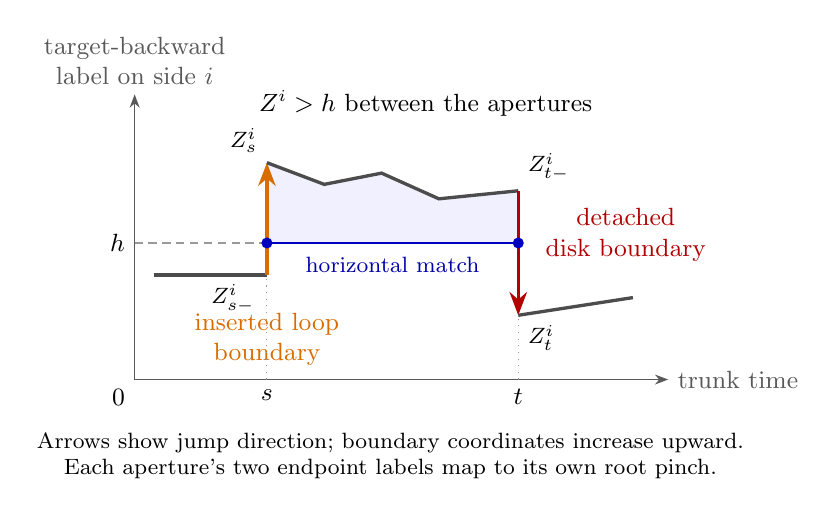
\begin{tikzpicture}[x=1.12cm,y=1.02cm,>=Stealth,
 every node/.style={font=\small}]
\draw[->,black!65] (0,0) -- (6.05,0) node[right] {trunk time};
\draw[->,black!65] (0,0) -- (0,3.55)
 node[above,align=center] {target-backward\\label on side $i$};
\node[below left] at (0,0) {$0$};
\fill[blue!6] (1.5,1.7) -- (1.5,2.7) -- (2.15,2.43)
 -- (2.8,2.57) -- (3.45,2.25) -- (4.35,2.35) -- (4.35,1.7) -- cycle;
\draw[very thick,black!70] (0.22,1.3) -- (1.5,1.3);
\draw[very thick,orange!85!black,->] (1.5,1.3) -- (1.5,2.7);
\draw[very thick,black!70] (1.5,2.7) -- (2.15,2.43)
 -- (2.8,2.57) -- (3.45,2.25) -- (4.35,2.35);
\draw[very thick,red!70!black,->] (4.35,2.35) -- (4.35,0.8);
\draw[very thick,black!70] (4.35,0.8) -- (5.65,1.02);
\draw[densely dashed,black!40] (0,1.7) -- (1.5,1.7);
\draw[thick,blue!75!black] (1.5,1.7) -- (4.35,1.7);
\fill[blue!75!black] (1.5,1.7) circle (2pt);
\fill[blue!75!black] (4.35,1.7) circle (2pt);
\node[left] at (0,1.7) {$h$};
\node[below left,font=\footnotesize] at (1.47,1.3) {$Z^i_{s-}$};
\node[above left,font=\footnotesize] at (1.5,2.7) {$Z^i_s$};
\node[above right,font=\footnotesize] at (4.35,2.35) {$Z^i_{t-}$};
\node[below right,font=\footnotesize] at (4.35,0.8) {$Z^i_t$};
\node[below,blue!65!black,font=\footnotesize] at (2.925,1.65) {horizontal match};
\node[align=center,above] at (3.3,3.15)
 {$Z^i>h$ between the apertures};
\node[orange!85!black,align=center,below] at (1.5,0.95)
 {inserted loop\\boundary};
\node[red!70!black,align=center,right] at (4.55,1.8)
 {detached\\disk boundary};
\node[below] at (1.5,0) {$s$};
\node[below] at (4.35,0) {$t$};
\draw[black!40,dotted] (1.5,0) -- (1.5,1.25);
\draw[black!40,dotted] (4.35,0) -- (4.35,0.75);
\node[align=center,font=\footnotesize] at (2.9,-0.95)
 {Arrows show jump direction; boundary coordinates increase upward.\\
 Each aperture's two endpoint labels map to its own root pinch.};
\end{tikzpicture}

\caption{A finite schematic of the boundary-label rule. At time $s$ a positive jump inserts a loop boundary; at time $t$ a negative jump removes a disk boundary. The level $h$ lies in both open apertures and strictly below the intervening extended graph, so the two marked labels represent the same boundary point by Lemma~\ref{proxy:stack-rule}. The endpoints of each aperture map to that aperture's own root pinch; no identification of the two apertures' endpoint pairs is asserted. Arrows show jump direction, while boundary coordinates increase from the lower endpoint of either aperture. The drawing represents neither a typical Cauchy trajectory nor Euclidean lengths or shapes of the welded surface.}
\label{fig:stack-labels}
\end{figure}

\begin{lemma}[Strict stack rule]\label{proxy:stack-rule}

For the almost-everywhere subcritical laws of Proposition~\ref{proxy:marked-factorization}, the following boundary-label inheritance rule holds.
Denote the remaining disks by \(D_t\), jump disks by \(C_t\) and the trunk tip by \(P_t\).
Use canonical prime coordinates in a starting post-state, at an ordinary deterministic trunk time (including 0) or at one of the above jump stopping times.
Boundary maps of remaining regions and offspring extend continuously in the original closed disk (the traces and their initial segments are continuous curves, have locally connected unions with the boundary, and the components have locally connected boundary).
In the starting disk's own coordinates subsequent bSLE branches are the ordinary continuous explorations, with continuous closure maps there as well.
Consider one side's boundary prefix from target back toward tip to length label \(h>0\).

\begin{enumerate}

\item Through a time interval on which the extension of that side's graph of lengths (including vertical jump segments, except possibly at specified endpoints) stays strictly above \(h\), the prefix is unhit, in correct \emph{access} in the subsequent prime frontiers.
On shared untouched open arcs its parametrization is inherited.

\item A positive jump inserts the full loop boundary interval from the pre- to the post-value in target-backward labels, with lengths as on the corresponding jump disk, cyclically from its root in the prescribed sense (so both endpoints have image the pinch).
At a negative jump, the interval from post- up to pre-value parametrizes in the corresponding sense the detached disk boundary starting and ending at its root.
Here the negative jump aperture notation uses length \emph{on that detached disk}; a comparison to earlier post-frontiers is on transmitted portions (it does not require a general continuity-of-boundary-chaos theorem on a pre-jump kernel limit).
If a strictly transmitted prefix has labels falling in the \emph{open} negative jump interval at its first loss, those labels are on this detached boundary with coordinate given by subtracting the post-value.

\end{enumerate}

Consequently strictly horizontal matches (staying strictly below the intervening path, between interior aperture/prefix labels) refer to the same actual points, with the stated prime-side inheritances, not just matching total masses.

\end{lemma}\begin{proof}

\proofstage{Protected prefixes and negative losses}

Work just after the specified start in its own canonical disk.
The target has an untouched neighborhood on every pre-terminal compact path segment.
Before any first intrusion, untouched open arcs use exactly the length inherited from this disk by collar comparison. A first hit into the interior of such an arc, coming from outside, separates the rest toward the tip on that side, making a disconnection event, i.e. a negative jump.
To formalize for a protected prefix, test with an intermediate endpoint \(h'\) slightly \emph{farther} than \(h\), still strictly below the graph; such test points can be chosen untouched.
Indeed in starting prime coordinates the continued exploration has the ordinary bSLE law, for which specified other boundary points are not hit (only the trunk could hit, as complete future loops are simple CLE loops).
Here one can use MSW's trunk law at skew zero, chordal \({\rm SLE}_{16/\kappa}(8/\kappa-3;8/\kappa-3)\), and the standard SLE with force points boundary-intersection theorem (in particular the boundary dimension bounds of Miller--Wu and related works): away from start and target, for an initial same-side weight strictly above \(\kappa'/2-4\), with \(\kappa'=16/\kappa\in(4,6)\) and the two tip weights \(>-2\) here, it is not boundary filling and has zero boundary Lebesgue measure there \citep[Theorem~1.6]{MillerWuBoundary}.  Indeed the boundary dimension at $\rho=\kappa^\prime/2-3$ is $1/2+1/\kappa^\prime<1$.
The one-side local bounds suffice (near a boundary swallow on that side localize away from opposite force points); Möbius covariance then gives avoidance of a given other point.
Even empty interior of the hit set suffices to choose untouched intervening labels, since boundary chaos in prime coordinates has full support without atoms.
These continuations need only be used from the countable post-state times under consideration. A first hit on the arc from target to \(h'\) then cuts off a nonempty boundary interval including \(h'\) on that side.
The post tip in the target component is at this hit with the access on the target side; that side length is exactly the coordinate of the hit.
For the last assertion, along the arc from the target the post domain has untouched access all the way up to the hit, converging there to the tip prime end, and in the cut domain the just lost part has access from the other direction also tending to its pinch prime end.
There is no extra split into different access labels at the hit in either component: in these starting-disk coordinates the prior trace avoids the hit until this first contact, is connected to the earlier start, and any two inequivalent accesses there joined by a simple interior curve from and to the point would bound a pocket in the disk with no prior trace inside (the trace is disjoint from that joining crosscut and the point until its terminal visit, and starts outside).
Hence the pocket lies in the component; equivalently the boundary interval between those accesses on the pocket side in Riemann coordinates would have constant image, impossible for a univalent map.
This also follows by trimming away from the approaching final trace and the untouched side arc.
Full bSLE excursions before contact are included in the connected trace argument.
Positive loops never intrude onto the starting boundary when they are in a fresh starting disk.
If a drop crosses \(h\) while a slightly longer prefix was preserved up to just before it, it must hit into that longer arc at the drop: otherwise the prefix would still give the lower bound (a disconnection swallowing the arc also requires such a hit between it and target).
The disconnection point's post length gives the claimed difference coordinate in the negative disk by the same shared arc rule.
This argument uses disconnection-post and cut markings at the jumps, covered by countable size-threshold lists \citep{MSWTrunk}.

\proofstage{The inserted loop and its two boundary measures}

For a positive discovery, the loop is attached at the trunk and in the post boundary, walking back from the tip on the insertion side traverses just the inserted loop first (two copies of the pinch); the interior is the corresponding \(C_t\).
These are the excursion and side conventions of bSLE, the loop other than its attachment being away from the previous compact trace.
More explicitly complete positive-excursion loops discovered strictly later than an ordinary surviving trunk time are still simple CLE loops in the unexplored target domain at that time, by the bSLE exploration property in those coordinates.
Use also countably many such times increasing toward the discovery; earlier contacts even at an eventual pinch would be excluded on these earlier pieces.
The only accumulation from the immediate approach is at the attachment by path continuity.
There is no simultaneous other detached open component at that time by the cut/jump correspondence and the Poisson/stable laws (two such positive-perimeter events do not coincide).
Thus away from the pinch along the simple loop the exterior access belongs to the post frontier, and the two disk sides there have local collars for comparing this actual seam \citep{MSWTrunk,MSWQuantum}.

Its length agrees on both sides not merely as a total but on open subarcs: use the DMS/Sheffield subcritical chordal quantum zipper \citep{DMS}\citep[Theorem~1.8 and Remark~5.7]{SheffieldZipper} (ordinary independent chordal \({\rm SLE}_\kappa\), \(\gamma=\sqrt\kappa\), weight-4 wedge into weight-2 wedges), which identifies lengths on the two sides.
This transfers locally to the present loop away from its start/end.
Indeed, viewed conditionally from rational capacity times during its tracing (also before any prescribed strictly interior subarc), bSLE until the excursion closes and away from the return point is ordinary simple chordal SLE with a boundary force/drift, locally absolutely continuous up to localized stops with separated driver points.
Its fresh open segment is interior in the then domain.
The parent field is independently, on interior compact subsets, a GFF plus a continuous correction up to change of law, and can there be compared by Markov coupling to the weight-4 zipper input (difference continuous on the neighborhood; local wedge chart and both fields couple via the same Dirichlet projection).
Condition first on the geometry up to the initial time for this comparison, then localize to subarcs in those neighborhoods and stopping bounds for ordinary chordal absolute continuity.
Zipper equality there concerns only that open part of the seam: completed ordinary-SLE collars from each side carry mixed-Neumann plus continuous regular arc charts, and other completions with the same local germ, including the actual loop cut/post charts, use exactly the same measures up to the exponential weight of the continuous field correction on the seam, by arc comparison.
One can phrase the localized transfer just as an assertion about smooth-kernel approximations on common side collars and thus needs no absolute continuity for the rest of the loop.
To detail that local comparison, condition at a geometry-only initial capacity time in an excursion, use an interior domain library for compact segments lying ahead away from the force coincidence, and couple the parent and zipper fields on the chosen neighborhoods by the same interior zero-Dirichlet projection there, first in reference field laws restoring independent average processes.
Those projections can be taken identical; the discarded harmonic fields, average substitutions and conformal terms are continuous in each interior neighborhood, and the disk bias can be included by absolute continuity.
Thus the zipper copy still satisfies its length equality there a.s.
One can first draw a common ordinary SLE segment independently, transfer up to localized separated-driver stops by chordal SLE drift absolute continuity, and then complete the actual exploration (the zipper conclusion was local to the compared seam with its own completion).
Simple-arc subcollars share the same side as these completions and use only those field restrictions, with the common continuous-surface correction on the seam.
Actual post and cut arc charts qualify for the earlier arc comparison by their disk marginals just proved; zipper charts away from their end marks similarly by wedge laws.
Countably many such compact-segment localizations cover the open loop arcs.
This applies first in typical-target coordinates, where the whole branch is independent of the parent disk field before clocking, to every excursion indexed using also field-independent rational times; almost-everywhere statements suffice for the above choice of approximations.
Endpoints have no atoms.
Together with the full signed jump rule this identifies the inserted interval as claimed.
\proofstage{Position and order of the inserted interval}

The open loop excluding the attachment is inside the pre-loop target component with closure based at a fresh tip, and is adjacent externally to the post component as above.
The attachment, fresh even through the immediate approach, has only one access in the pre-loop target component.
Indeed two accesses joined by an interior Jordan arc from and to that point would enclose a pocket missing the earlier connected trace (which starts on the outer boundary and avoids the point until then), again impossible by nonconstancy on prime intervals.
Thus in pre-loop prime coordinates the circle can only add a boundary detour from and back to that tip, with the post tip at one of its ends.
Its open arc carries equal interior/exterior length by the preceding comparison, so the detour at the top of that post side has exactly the jump magnitude.
The rest of each post side, before this detour as applicable, has length at least the corresponding pre-value: indeed work in a sufficiently close preceding post-state (ordinary times increasing to the event suffice), where prefixes strictly short of those pre-values stay protected up to insertion and persist still outside the detour since the new loop is interior relative to that state.
Total length increase now gives equality and the side/order convention as claimed.
Horizontal comparisons from a positive aperture just start in its post-state with inherited labels.

\end{proof}

\subsection{A strictly subcritical metric proxy}\label{proxy:metric}

To control actual access maps (mere interior kernel convergence is not a priori enough), fix an auxiliary strictly subcritical LQG metric with parameter \(\gamma_0=\sqrt{8/3}\), charge \(Q_0\), metric exponent \(\xi_0=\gamma_0/4\).
We use the subcritical metric construction and its LFPP realization \citep{GMMetric}, together with the weak-metric moment estimates of Dub\'edat--Falconet--Gwynne--Pfeffer--Sun \citep[Theorem~1.9 and Proposition~3.1]{DFGPS}.  The inputs are $\xi_0Q_0=5/6<1$, scaling and Weyl scaling, and upper moments of all orders for internal annular/path-around costs and inverse moments of all orders for across-annulus costs on fixed interior annuli in a whole-plane GFF with fixed circle constant.
Fixed internal box-crossing upper estimates used below follow by chaining finitely many such short winding paths over overlapping interior annuli with forced intersections.
The theorem of Devlin on simultaneous conformal coordinate change is used \emph{only for this strictly subcritical proxy}.
In a fixed bounded parent disk coordinate \(\Delta\) (unit disk), use \(D^{(0)}_{h_{\rm parent}}\) as local/intrinsic proxy metric.
If \(F:{\cal S}\to U\subset\Delta\) is a jump disk or jump-post-state map in standard marked coordinates as above, the internal proxy pullback has length element that of \(D^{(0)}_{g}\) weighted by \(|F'|^{\xi_0(Q_0-Q_\gamma)}\), where \(g=h_{\rm parent}\circ F+Q_\gamma\log|F'|\) is the actual disk field.
Since \(Q_0>Q_\gamma\) here, Cauchy estimates give the deterministic upper weight bound \(C(\min(1,\operatorname{dist}(\cdot,\partial{\cal S})))^{-\xi_0(Q_0-Q_\gamma)}\).
The same applies to compositions of such maps into the fixed parent chart \citep[Theorem~1.9 and Proposition~3.1]{DFGPS}\citep[Theorem~1.1]{Devlin}.

Here are details about the randomness in this metric comparison.
For a branch toward a typical target choose parent charts from its start and target, with deterministic strip-to-disk convention.
Conditional on the full \emph{unclocked} bSLE branch, independent of the parent field, all countably many domains of jumps and jump-post states can be treated by ordinary fixed-map covariance, mapping first from a canonical disk by geometry-only choices.
Indeed they come from the geometry of loop closures and disconnections alone.
Conditional on it, on each domain the parent field and pullbacks qualify in law up to absolute continuity as a whole-plane GFF plus a (random) continuous function in its interior: use the lateral strip description, add back and remove an independent average, use Neumann/Dirichlet Markov comparison (free GFF has independent Dirichlet projection plus harmonic distribution in the \emph{open} subdomain), then whole-plane/Dirichlet comparison and charge correction; normalization/tilt is continuous addition/change of law.
After fixed geometry-only comparison, the remaining h-dependent re-embeddings change only standard disk coordinates by conformal maps between \emph{fixed} domains, for which use Devlin's simultaneous rule on the disk.
At the random standard chart on the child side the field with proxy charge is \(g+(Q_0-Q_\gamma)\log|F'|\), with the same qualification now by the marked disk marginal law; its metric and that for \(g\) therefore are related by the usual continuous Weyl length factor even here.
To clarify this last version argument, the subcritical metric on each fixed domain in these laws agrees locally with the normalized LFPP limit length element (one can use the localized dyadic approximants).
For a whole-plane GFF plus continuous this is the subcritical LFPP convergence/metric identification, and on any coupling having two such qualifying marginal laws differing by a random continuous function the two elements of length differ by the exponential weight: locally the approximating mollifier weights sandwich with arbitrarily small oscillation error.
Locally uniform distance convergence suffices for this comparison, by first confining short distances within compact neighborhoods via the positive exit cost, passing the sandwich for nearby pairs, and subdividing compact paths.
One may equivalently apply the pathwise continuous-addition construction of the metric from LFPP; convergence/identification on local compact neighborhoods transfers under absolute continuity.
This uses Devlin as a \emph{version of} the metric on the fixed standard domains, avoiding evaluation of a version on a field-dependent domain outside its scope.
Thus arbitrary changes between qualifying standard parent charts for these branches cause only the corresponding analytic/Weyl terms.
In particular the a.s. comparisons transfer also if using a fresh typical mark with the source for the parent chart, and then for almost all the above subcritical perimeter/split prescriptions in this chart.
In successive cuttings apply it one step at a time in the marginal parent/branch laws, transporting earlier derivative weights by path composition.
We will use this also directly at critical charge 2 only for analogous branch laws when the independent geometric branch and actual marked offspring laws there have been established (the proxy still subcritical) \citep[Theorem~1.1]{Devlin}.

\begin{lemma}[Uniform lower cost for macroscopic paths]\label{proxy:lower-cost}

In a unit disk parent chart obtained from standard strip coordinates with typical source and an auxiliary or target typical mark and perimeter 1, paths in the open disk of macroscopic Euclidean diameter cannot have arbitrarily small internal proxy length, uniformly in probability as \(\gamma\) increases.
The assertion is uniform when the perimeter belongs to a compact subset of $(0,\infty)$. 

\end{lemma}\begin{proof}

On interior compacta this is ordinary metric positivity and tight continuous corrections; in bounded horizontal slabs up to the strip edge it suffices to rule out arbitrarily cheap paths close to the boundary crossing a fixed interval tangentially.
For each fixed horizontal coordinate \(x\) on that interval, consider interior Whitney boxes above \(x\) at small depths \(e^{-n}\), with finitely many per level, arranged so any path hitting the normal above \(x\) at such depths and exiting its Whitney neighborhood (size at most \(C\) times depth) must cross one interior annulus of size \(\asymp e^{-n}\).
In the straight local chart their proxy charge scaling is \(e^{\xi_0(H_n-Q_0 n)}\) up to tight coarse continuous factors, times annular costs with uniform inverse moments.
The latter fact follows by rescaling the Neumann field minus semicircle average (bounded harmonic Gaussian corrections on the rescaled interior boxes) and the stated interior metric estimates.
The deterministic parent chart derivative correction on the slab is bounded.
Since \(H_n/n\to0\) in probability uniformly over all large \(n\) at fixed \(x\), with summable Gaussian error tails, and \(\xi_0Q_0<1\), with uniformly high probability at fixed \(x\) all these small crossings cost at least \(e^{-n}\) (the DMS tilt and random coarse corrections can first be truncated).
Fubini gives a good set covering most of the fixed interval in Lebesgue length.
Hits by a path confined to the thin collar and traversing tangentially thus force total length bounded below: select disjoint horizontal Whitney neighborhoods of hits on good normals with sum of widths bounded below by interval covering (use a strictly interior subinterval to ensure exits).
Paths that do not remain in a thin collar already have an interior macroscopic traversal.
Any macroscopic movement on the compact disk boundary contains tests away from the two ends, covered by finitely many such slab tests.
This proves the estimate.

\end{proof}

\begin{proposition}[All-point boundary-chain estimate]\label{proxy:boundary-chain}

For a disk \(g\) in standard twice-typical strip coordinates with perimeter \(s\), paths in its interior approaching any flat boundary point \(z\) and \(+\infty\) can be joined, along the direction to the right, at cost bounded (including the above deterministic upper weight) by

\begin{equation}
K\,s^{2\xi_0/\gamma}\left(\frac{m([z,+\infty))}{s}\right)^{\theta 2\xi_0/\gamma},
 \label{eq:original-11}
\end{equation}
where $m$ denotes boundary length on that side.  The moment quantifier is as follows: for each $M\in(0,\infty)$, choose $\theta<1$ sufficiently close to $1$ and then $\gamma_M<2$ so that
\[
 \sup_{\gamma\in(\gamma_M,2]}\E[K^M]<\infty.
\]
The value $\gamma=2$ denotes the limiting disk law.  The choice of $\theta$ is allowed to depend on $M$.
More precisely we assert existence of connected chains/paths \emph{between arbitrarily small neighborhoods} of the two points, simultaneously at every \(z\).
The reverse statement toward \(-\infty\) also holds, and the chains may approach an end on either side using central Whitney slab paths.
No exact internal metric extension to boundary is needed.

\end{proposition}\begin{proof}

We prove \eqref{eq:original-11}.
On a unit slab use first the mixed/free GFF boundary model above, writing \(H_n(x),X_n=2n-H_n(x)\) with the previous reference.
Cover a boundary interval by mesh points at each scale \(e^{-n}\).
Chains to larger scales above any point of the interval can be made by short crossing and surrounding paths in interior Whitney boxes: for instance place annuli about an interior point at height \(c e^{-n}\) above each mesh center, with radii small multiples of that height, and connect by chains of overlapping annuli in the comparable-depth neighborhood to the possible next coarser centers, using forced crossings and staying at comparable height.
Windings at successive levels and these bridges join; finitely many configurations at each center suffice.
Centers of boxes need not lie directly to the right of the desired point.
Charge the estimate at scale \(e^{-n}\) against the mass of a short boundary interval at displacement \(+C e^{-n}\) on the same side from its grid center, so all charged intervals are within a bounded distance to the right of the limiting \(z\).
Under the endpoint tilt by \(H_n\), the mass divided by \(e^{(\gamma/2)(H_n-Q_\gamma n)}\) has inverse moments of all orders as proved above, and the crossing costs (summing the finitely many tests at this center) with the derivative upper weight, divided by \(e^{\xi_0(H_n-Q_\gamma n)}\), have positive moments of all orders.
Indeed without the derivative weight use the standard rescaled interior metric estimate with \(Q_0\); interior harmonic-field corrections after subtracting the coarse semicircle, including the tilt shift, have uniform exponential moments.
Thus the cost bound at the center divided by the indicated short mass to power \(\theta 2\xi_0/\gamma\) is at most
$Y_n e^{-dX_n}$, with $d=(1-\theta)\xi_0>0$ and $Y_n$ having uniform moments of all orders under the tilt.  Indeed, the exact remaining exponential factor is $e^{-d[X_n+(Q_\gamma-2)n]}$, which is at most $e^{-dX_n}$ because $Q_\gamma\geq2$.

\smallskip\noindent\textit{Uniform control of all chains and visit counts.}\quad

Here are details for summing these charges on all boundary chains.
Use the simultaneous barrier with parameter \(y\ge1\) already proved.
Except for probability \(C_d(1+y)^C e^{-y}\), at all grid points in the band \(X_n\in[-y+j,-y+j+1]\) with barrier survival, \(j\ge0\), we have \(Y_n\le C_d e^{d j/4}\) and oscillation \(O_n\le C+j/3\) up to fixed mesh multiples.
Indeed sum the undo-tilt bounds with cost \(C e^{-y+j}\), using the high-moment/Gaussian tails and saving ballot power \(b>2/3\).
Thus along chains using nearest mesh centers at each scale, ratios are bounded by \(C_d e^{dy}e^{-d(X_n(z)+y)/3}\).
We next bound the number of levels at which a chain comes close to the
barrier.  Work first on the simultaneous barrier and oscillation event just
constructed.  Suppose that, for some boundary point $z$, the quantity
$X_i(z)+y$ visits $[0,J]$ at more than $A(J+1)^4$ levels, and let $n$ be a
level at which this bound is first exceeded.  Choose a mesh center $x_n$
within $e^{-n}$ of $z$.  At every earlier level $i\leq n$, both points lie
within a fixed mesh multiple of the same level-$i$ center.  The oscillation
bound, solved for that center's height, shows that every counted visit
gives
\[
 0\leq X_i(x_n)+y\leq C'(J+1).
\]
The lower inequality at all other levels follows from the simultaneous
barrier.  In particular the endpoint at level $n$ belongs to this same
bounded band.  This is a pathwise implication on the good event.  Having
obtained it, we drop that event and estimate the resulting event at the
fixed mesh center $x_n$.

Under the endpoint tilt by $H_n(x_n)$, put $W_i=X_i(x_n)+y$.
Its increments form the centered variance-$2$ Gaussian walk, and its
starting height is $y$ plus the bounded Gaussian correction used in
Lemma~\ref{proxy:barrier}.  Let $V_J$ count its visits to
$[0,C'(J+1)]$ before killing below zero.  This count has an exponential
upper tail on the $(J+1)^2$ scale, uniformly in the starting height.
Indeed, start the first block at the first visit to the band, give it
$L_J=\lceil C''(J+1)^2\rceil$ steps, and start each subsequent block at the
first later band visit.  From every point of the band there is a
probability at least $c>0$, independent of $J$, of being killed during that
block.
Each block contains at most $L_J$ counted visits.  The strong Markov property
therefore gives
\[
 \Prob_*(V_J\geq k)\leq C\exp\{-ck/(J+1)^2\}.
\]
At $k=A(J+1)^4$, combine this estimate with the endpoint ballot bound by
H\"older, retaining a ballot power $b>2/3$.  Undoing the tilt and summing over
the $O(e^n)$ possible centers gives the same factor $e^{-y}$ as before.
The endpoint bands cost at most $e^{C'(J+1)}$, whereas the visit estimate
contributes $e^{-cA(J+1)^2}$ after adjusting $c$.  The sums over $J$ and over
$n$, the latter bounded by
\[
 \sum_{n\geq1}n^{-3b/2}(1+y+\log(2+n))^C,
\]
are finite.  Thus, outside an event of probability
$C_d(1+y)^Ce^{-y}$, every boundary chain has at most $A(J+1)^4$ visits to
$[0,J]$, simultaneously for all integers $J\geq1$.
Let $A_*$ be the supremum of the summed cost ratios over all boundary
chains in the slab.  The preceding bounds give
\[
 A_*\leq C_d e^{dy}\sum_{J\geq0}(J+2)^4e^{-dJ/3}<\infty.
\]
The bound $\Prob(A_*>C_de^{dy})\leq C_d(1+y)^Ce^{-y}$ gives
$\E A_*^q<\infty$ for every $q<1/d$.  Since $d=(1-\theta)\xi_0$, choosing
$\theta$ sufficiently close to one supplies any prescribed moment, with
room for the H\"older inequalities used to restore the radial part.

Finitely many larger-scale slab-interior crossings to link these chains and move right one slab are handled the same way without level summation, charged against a fixed interval still to the right.
They can use common surrounding paths to connect the choices.
Enlarge $A_*$ to include these finitely many links; the same moment bounds
continue to hold.
All these estimates hold for \(P^\perp\) by the compact slab continuous Gaussian corrections.

\smallskip\noindent\textit{Restoring the radial part and the perimeter.}\quad

Restore the radial and normalization factors: per slab needed to go right from \(z\) (including the starting one) the cost is at most the right side of \eqref{eq:original-11} with \(K\) replaced by
\[
 C\,A_k V_\gamma^{-(1-\theta)2\xi_0/\gamma}
 \exp\{-d\,U_a(k)+C\,{\rm osc}_{[k-C',k+C']}U_a\}.
\]
Indeed each compared mass interval is inside the indicated tail; \(A_k\) depends only on the lateral field with the above moment control and bounded normalization-unit constants.
Sum the bounds over all \(k\): the sum of the displayed exponential occupation factors alone has all positive moments uniformly.
For integer moments order tuple times, group overlapping bounded windows (groups still bounded for fixed order), and use at each next separated group the Gaussian density bound \(C(1+m)^{-3/2}\) for the 3-dimensional drifted motion across gap \(m\), integrating the exponential radial decay with bounded-window supremum-increment exponential moments.
The two halves cause no change.
Conditional Minkowski over the lateral field therefore preserves the desired large moments of the \(A_k\)-weighted sum, with slack for Hölder with inverse \(V_\gamma\) (all orders by one slab and radial bounds), and the small positive DMS tilt.
This proves \eqref{eq:original-11}.
The same proof works at limiting charge, with limiting normalization constants.

\end{proof}

\subsection{Uniform boundary continuity and small images}\label{proxy:consequences}

Consequences are used in the following probabilistic sense.
Boundary arcs of small relative length incident to a typical boundary mark have images of small diameter, with the exceptional upper-chain probability at any fixed proxy threshold a power of relative length of arbitrarily high prescribed order, times the corresponding perimeter scale factor.
If an arc passes the second typical strip mark, use \eqref{eq:original-11} at both ends.
To treat \emph{all} arcs of a given size discretize by a mesh of that size from a uniform length origin, each anchor again marginally typical after disintegrating the cut process as necessary; use coordinates based on each anchor.
This loses only one power for the grid union.
The whole boundary can also be covered with cost scale \(s^{2\xi_0/\gamma}\), with such moments.
In these assertions the upper costs just require paths between near-boundary points in the open parent; passing through Lemma~\ref{proxy:lower-cost}, a single high-probability lower bound in the parent, gives the actual Euclidean smallness simultaneously, using continuous closure maps.
Whole-domain diameter then follows also by the maximum principle.
Equicontinuity in prime coordinates of disks with lengths in compact positive ranges follows in probability by the above and convergence of the standard-coordinate boundary measures to diffuse full-support measures; bounded analytic maps with equicontinuous boundaries are equicontinuous on the closed disk.
None of this asserts independence of coordinates of the embeddings from the cut surfaces used for \eqref{eq:original-11}.


\section{Critical cutting, Palm comparison, and peeling}\label{sec:cutting}

This section connects the critical disks of Section~\ref{sec:proxy} to the
independently constructed sphere of Section~\ref{sec:continuum}, and then to the
exact map law of Section~\ref{sec:discrete}.  We first identify the critical
exploration together with every boundary contact.  We next identify the
counting intensity of sphere cuts, including its normalization.  Finally we
couple the exact peeling operations to these cuttings and obtain spatial
comparisons for all flag incidences, before and after exact volume conditioning.

Throughout the continuum approximation,
\(\kappa=\gamma^2\uparrow4\), \(r=4/\kappa\downarrow1\), and
\(a=Q_\gamma-\gamma\).  The disk area and boundary-length units are those of
Section~\ref{sec:proxy}.  The processes below describe the two actual sides of
a branch; their geometric identification is part of the proof.

\subsection{The critical branch and its contact relation}\label{cut:branch}

\begin{lemma}[The corner lifetime]\label{cut:lifetime}
Let the raw process have two independent symmetric Cauchy coordinates,
each with Lévy measure \(du/(2u^2)\), and kill it upon leaving the positive
quadrant.  Its Doob transform by \((x+y)^{-2}\), started from any
\((x,y)\in(0,\infty)^2\), has total mass one up to a finite lifetime \(T\).
For \(S_t=Z^L_t+Z^R_t\), one has \(S_t\to0\) as \(t\uparrow T\) and
\(\E T\le C(x+y)\).
\end{lemma}
\begin{proof}\leavevmode

The candidate length law is the Doob transform of two independent symmetric Cauchy processes (each density \(du/(2u^2)\)), killed outside the positive quadrant, by \(S^{-2}\), run to the corner. Here are lifetime details. At \(S=1\), twice the killed generator of \(S^{-2}\) is
\[
 \sum_{\ell=x,y}\left\{{\rm PV}\int_{-\ell}^\infty
 \frac{(1+u)^{-2}-1}{u^2}\,du-\ell^{-1}\right\}=0
\]
(each term is \(2\log(\ell/(1-\ell))+1/(1-\ell)-1/\ell\)).
Replacing \(-2\) by \(-1\) gives \(\sum(\log(\ell/(1-\ell))-1/\ell)\le-4\).
Scale homogeneity therefore gives transformed drift of \(S\) bounded above by a negative constant.
These calculations apply up to quadrant compact exits by Lévy optional stopping, including overshoots with the actual function value (zero outside; exits from pre-sides \(\ge\epsilon\) leave at least one side \(\ge\epsilon\), so the harmonic density stays bounded).
Thus there is a consistent probability law until leaving all compacta, with mean lifetime bounded by \(C S_0\) and \(S\) a supermartingale there.
Exits cannot run to infinity, nor leave through an individual axis while \(S\) stays positive: localized with \(S\) away from zero the density at inner side exits with \(S\) still bounded below is bounded, and on finite time windows a raw one-dimensional Cauchy process almost surely never hits a specified point by value or left limit (polarity, including jump pre/post values by the Lévy measure).
Jump exits outside are given zero weight.
Finally from arbitrarily small \(S\) returns to fixed large size before lifetime have probability bounded by the supermartingale estimate.
Thus almost surely \(S\to0\) at finite lifetime \(T\), and the localized laws exhaust unit mass.

\end{proof}

\begin{definition}[Side contours and the contact relation]
\label{cut:contact-relation}
Let $Z$ have the length law of Lemma~\ref{cut:lifetime}.  For each side
$\alpha\in\{L,R\}$, form an ordered contour by first following the original
boundary from target to source, with height increasing from $0$ to
$Z^\alpha_0$, and then following the side's length path from time $0$ to
$T$.  Fill every jump by its vertical height interval and give these
intervals positive summable traversal durations.  The resulting height
function $e_\alpha$ is continuous, is positive away from its two target
ends, and vanishes at those ends.

Two occurrences $u\leq v$ on this contour are directly linked if
\[
 e_\alpha(u)=e_\alpha(v)
       =\min_{w\in[u,v]}e_\alpha(w).
\]
The vertical interval at a jump is the aperture of that jump.  Its two
endpoints represent the same pinch; its open interval parametrizes the
jump-circle boundary away from the pinch.  At an ordinary real time there
is one tip copy on each side; at a jump the jumping side has a pre- and a
post-copy.  All tip copies of the same real time represent that time on
the trunk.  The source and target carry their usual endpoint copies.

The \emph{contact relation} is generated by the direct side linkages and
these tip and endpoint identifications.  It is a relation on occurrences,
so it does not presume that the corresponding embedded points coincide.
\end{definition}

\begin{proposition}[Critical cutting and the exact contact rule]\label{cut:critical-cutting}
Consider a critical field disk with a boundary-typical source and a target
at any prescribed strictly interior relative boundary length.  Its independent
symmetric \(\mathrm{bSLE}^{0,0}_4\) exploration admits a trunk-time
parametrization in which the left and right boundary lengths have the law of
Lemma~\ref{cut:lifetime}.  Conditional on the full length path, the jump
interiors are independent critical disks with the corresponding perimeters
and pinch marks.  At the compact-surviving deterministic times and selected
jump stops used below, the remaining disk has the marked disk law conditional
on the observed past length data.

The trunk is a simple continuous arc, all jump domains are Jordan domains,
and two contour occurrences have the same physical image exactly when
they satisfy the contact relation of Definition~\ref{cut:contact-relation}.  In particular no side class links two distinct real trunk times,
no class identifies distinct points of one outer or jump circle, and no
inserted positive circle visits the original boundary.  The full exploration,
including its ordered loop tours, is obtained as the limit of the subcritical
cuttings on compact surviving pieces, with the terminal remainder shrinking
spatially to the target.
\end{proposition}
The proof has three components.  We first construct subsequential limits
of the actual maps and traces.  We then prove that their contact relation
is exact.  Finally the Loewner driver identifies the limiting exploration
and its conditional disk laws.

\begin{lemma}[Compact-survival limits of the marked cuttings]
\label{cut:compact-geometric-limit}
Let good subcritical starting pairs converge to a positive critical pair,
and use the standard parent charts of Section~\ref{sec:proxy}.  Every
sequence has a subsequence on which the localized length-path couplings
extend jointly to the actual jump and post maps and the trunk.  The maps
converge uniformly on their closures and do not collapse; the trunk limit
is continuous and has no constant interval.  Small jump domains shrink
uniformly on compact surviving pieces, and the terminal remainder shrinks
to the target.  The positive jump boundaries are distinct simple
$\CLE_4$ loops.  The marked disk laws hold on every retained finite
past-length test, with the conditional scopes of
Proposition~\ref{proxy:marked-factorization}.
\end{lemma}
\begin{proof}


\proofstage{Localized convergence and stopping selections}

As \(r\downarrow1\), the subcritical strictly stable pairs converge locally in \(J_1\) before change of measure (the positive imbalance is \(O((r-1)^2)\), so even the compensation from large jumps converges without residual drift).
Hence the Doob laws on any pre-terminal compact path cylinder with null threshold boundaries converge with their weights, and the same is true jointly for the abstract jump and post disk laws on these pieces, by the preceding disk limits.
Here the (good subcritical) initial splits can tend to any desired critical pair in the open quadrant; positivity tests use strict interior compact ranges, or one conditions/exhausts by these.
There is no loss of probability by considering just such pieces up to post-jump times where \(S\) is small, because the candidate above has total mass one, reaches such times in countable threshold tests with probability tending to one (jumps are dense), and the \emph{entire remainder} at the corresponding subcritical jumps has diameter tending to zero in probability as the threshold for \(S\) tends to zero by \eqref{eq:original-11}.
This last assertion uses post disk law and a selectable stopping test bounded in time while the pre-stop path stays in a fixed positive compact set for each fixed cutoff test; one may also exhaust the selection by a bounded list and use disintegration at each first suitable jump.
Estimate \eqref{eq:original-11} conditional on the split/path supplies the upper costs with probability tending to one at rate a power of the small perimeter, independent of the number of steps for a stopping choice (the parent lower proxy test is made separately).
The remainder contains the terminal target in its closure.

For clarity these localized convergence arguments can be implemented by coupling along further subsequences of any input sequence: keep countably many finite time windows, side-range cylinder cutoffs and enumerated jumps bounded away from zero therein (choose thresholds off atoms), with marginal convergence on these compact-survival events.
One can place states at rational time horizons in a stopped path space with a default symbol if the path has already left the corresponding cylinder.
Cylinder masses and joint laws for all coarser initial pieces inside such cylinders converge by the bounded-density path transfer, including the stopped first-exit prefixes on smaller cylinders when needed.
Equivalently, for each accuracy first couple on finitely many disjoint compact-survival tests whose limit probabilities already sum to \(1-o(1)\) and which together continue through a selected tiny-\(S\) jump; then diagonalize accuracy.
Such disjoint tests are formed by rational bounds on duration and side extrema (including left limits), and testing the tiny-\(S\) entry using paths up to that bound (or first passing a jump threshold); priority for testing earlier entries can be imposed using only prefixes.
Failure to extend farther in the approximants never removes mass from a common prefix in a strictly positive cylinder.
This is a liminf/saturation use of compact convergence; it does not posit convergence of terminal durations at the singular corner.
Jointly bounded-coordinate field objects, paths and embeddings on the pieces need tightness, as follows.

In these localizations bounded-weight transfer works up to a first selected jump before a finite bound while pre-path and post-value stay in positive compact side ranges.
One way to see it just using deterministic horizon laws is to round that first jump time from above by dyadic times, requiring survival until then in a slightly expanded cylinder.
Right-continuity gives exhaustion at the actual stop for every counted compact-surviving path, and on the raw side the terminal density converges boundedly to the value using the jump-post position.
Equivalently stop the localized Doob law there.
For convergence across parameters, threshold/entrance and range tests up to the stop (including pre/post side sizes, the absence of earlier qualifying jumps etc.) can be chosen off all discontinuity boundaries in the raw limiting path; a fixed jump threshold has only finitely many candidates there before the time bound.
Thus this convergence of restricted finite measures applies also to their paths, and the disintegrated marked laws at those stops use the disk estimates uniformly in the selected lengths.
In particular one can use a \emph{single stopping selection} for each desired tiny bound \(\delta\) on \(S\), e.g. first jump above a lower threshold in absolute magnitude with small enough positive post-\(S\), before a sufficiently large fixed time and under pre- and post-compact survival bounds.
Choose these subsidiary thresholds (with strict margins, then allowing the compacts to increase for each fixed desired accuracy) so that existence has probability tending to one under the limiting transformed law, by jump density and \(S\to0\) only at terminal.
Conditional upper-chain bounds at this selected stop need not pay once per candidate.
The selected times in the candidate law eventually cover each initial compact piece as the tiny bound vanishes.
For post-map tests at other individual jumps on a fixed compact window, extra future success conditions need not be imposed when bounding bad-map probabilities: sum bounds at the jump stops themselves restricted to positive compact prefixes, controlling candidate counts there by the bounded-density and jump intensity estimates.
On projecting to a fixed matched post or cuts and length data up to their horizon, the marginal marked rule in any final subsequential limit follows by testing on these fixed compact-survival events in the approximants, whether or not maps from several different times were jointly kept.
Omitting outcomes failing the final tiny-\(S\) tests costs vanishing probability.
This use of exhaustion/couplings needs only convergence on initial segments; in expanding by excursions and passing to full curves the terminal remainder is controlled spatially, not by bounding its duration.

\proofstage{Tight closure maps and noncollapse}

Embed the original disk in \(\Delta\) in standard perimeter-normalized twice-typical coordinates (ignore the prescribed target for this choice if needed).
All individual jump offspring and post states on the tests above, mapped into \(\bar\Delta\) in their own corresponding standard coordinates, are tight in the uniform topology by \eqref{eq:original-11}; they are noncollapsed in subsequential limits.
Indeed their areas on inner compacta are tight with nonzero limiting mass, these are actual parts of the original area by interior covariance, and the parent measures converge to diffuse measures.
Interior field pullbacks therefore have the genuine charge-2 relation in the limit by univalent compact convergence, and lengths in each chart are the stated critical disk lengths.
Different jumped-away disk interiors remain disjoint and are avoided there by all past/future remaining traces (interiors persist by uniform compact convergence).
Taken collectively, small jump-disk maps on compact path intervals shrink in maximum diameter: use \eqref{eq:original-11} for the whole boundary with expected power sums of small jump sizes on the positive compact path tests bounded by stable-process sums of powers \(p>r\), tending to zero for a vanishing jump threshold.
The same argument can transfer high-probability short-arc tests on countable jump-post lists; moment orders in \eqref{eq:original-11} can be chosen arbitrarily high.
Shrinking here and below takes place jointly using Lemma~\ref{proxy:lower-cost} once in the ambient chart, then short-cost upper tests.

\proofstage{Oscillation of the actual trunk}

We verify tightness of the actual \emph{trunk in trunk time}, not just of the domains.
On compact-survival intervals partition at successive jumps of size \(>\delta^R\), with fixed \(R>1\); include the initial state and, if stopping at a selected jump, end the last interval there.
For each fixed compact cutoff under consideration, with probability tending to one as \(\delta\to0\) there are \(O_{\mathbb P}(\delta^{-Rr})\) such intervals and both side lengths oscillate by \(<\delta\) between the initial post-state \(a'\) of each and just before its last jump \(b'\) (different constants in front of \(\delta\) would work too).
For example under the base laws the longest gap before a bounded horizon is at most \(O(\delta^{Rr}\log^2(1/\delta))\) with high probability.
Compensated smaller increments have variance rate \(O(\delta^{R(2-r)})\) and jump bound \(\delta^R\), hence exponential maximal bounds by Lévy exponential tilting on blocks of that length; the remaining skew drift has size at most \(O(\delta^{R(1-r)})\) uniformly.
Transfer on the cylinder.
By \eqref{eq:original-11}, all length-\(O(\delta)\) arcs on the post and terminal jump frontiers under test have simultaneously vanishing image diameter in probability.
For jump disks of sizes \(s\) possibly much smaller than the side lower bounds, use the whole-boundary estimate if \(s\lesssim\delta\), otherwise \eqref{eq:original-11} with relative size \(C\delta/s\), bounded perimeter factor and the grid union.
The polynomial number of tests costs nothing with sufficiently high moments.

In the canonical starting disk at \(a'\), near-full prefixes (leave \(C\delta\) gap to the tip) on both sides are then untouched until \(b'-\). The non-inherited arcs of the boundary of \(D_{b'}\) are short, with the following jump qualifications.
\begin{itemize}
\item At a positive terminal jump one inserted aperture may be large; join back \(C_{b'}\) along that aperture, whose open seam outside the pinch has a collar on both sides and was not encountered earlier.
\item At a large negative jump the hit is on an untouched prefix; the long segment of \(\partial C_{b'}\) from that hit back toward the old tip (ending on the prefix) is inherited, and all the rest of that detached boundary has length \(O(\delta)\). At a small negative jump the whole detached boundary is small.
\end{itemize}
In all cases the omitted \(O(\delta)\) arcs at \(a'\), all the changed short arcs at \(b'\), and both tips are inside a parent ball of small radius tending to zero under our tests: they link by common inherited prefix endpoints and common pinches.
The descriptions follow from the strict stack rules of Lemma~\ref{proxy:stack-rule}, choosing margins off the fluctuating side lengths before the last jump; in the borderline case of a negative loss within that margin use only shorter prefixes and the small jump bound.

No intermediate macroscopic finger of the trunk or removed material (except the cell at the last jump itself) can then lie outside this ball, enlarged a little.
Indeed in the open canonical disk of \(D_{a'}\), consider each component outside its pullback under the parent embedding.
The boundaries of the post and terminal jump domains there have no interior portions except, in the positive case, the shared open seam just described.
Thus a component is wholly retained in their union (including this seam), or would be wholly discarded.
Any discarded component must have an access adjacent to an untouched/inherited old boundary point mapping outside the ball: otherwise its whole boundary in the closed disk maps inside the closed ball, impossible by the maximum principle.
At such a boundary point the post or terminal jump domains have genuine inherited collar access on this starting-disk side, contradiction.
Boundary contacts outside the ball at earlier times are likewise excluded by prefix protection.
The interiors of post and last-jump domains are never touched on the trunk interval and the large positive seam is first reached at the last tip only.
This proves the claimed tip oscillation up to and including the terminal pinpoint on each interval.
For fixed mesh parameter successive large jumps are separated in time in the localized limit.
Thus these oscillation controls prove tightness with continuous limits under the \(J_1\) path couplings of lengths.
At the end, after tiny-\(S\) localized stops as above, all remaining tips and jumps are confined near target.

Pass now to joint limits on these pieces, using time homeomorphisms as needed for \(J_1\).
We have a continuous limiting trunk \(P\) up to and including \(T\), continuous closure maps with inherited disk laws at jumps, and a full continuous path obtained by interspersing the positive loops, traversed in boundary-length order of the corresponding orientation.
This last path also has uniform convergence modulo time change: give positive auxiliary durations to the positive jumps summably in their countable matched order, or match just finitely many large ones at each accuracy, using small diameters and trunk continuity for the rest.
The trunk avoids jump-disk interiors by approximation.
Every positive loop here is a distinct simple outermost loop of a genuine \({\rm CLE}_4\) in \(\Delta\).
Indeed consider also the parent non-nested CLEs through their domains at countably many interior tests.
These domains converge in kernel law to those of \({\rm CLE}_4\): by the Sheffield--Werner Brownian loop-soup construction \citep{SWcle} they may separately for this assertion be coupled increasing at each interior point as soup intensity increases, and the Schramm--Sheffield--Wilson conformal-radius law \citep{SSWradii} is continuous up to \(\kappa=4\).
Thus the increasing kernels exhaust the final interiors (strict radius monotonicity); prescribed interior points lie in loop interiors almost surely.
This is tight joint data before any localization.
Each positive jump domain contains a rational interior point stably, so equals in its interior limit the corresponding kernel, by its uniformly convergent univalent map, and distinct ones have disjoint interiors.
Its boundary map thus parametrizes the simple CLE boundary homeomorphically.
Consequently \(P\) has no constant intervals, since distinct disjoint simple loops attach on any such interval by positive-jump density.


\proofstage{Consistency of the limiting data}

The compact extractions can retain all the path data consistently.
Localized extractions as above need only tightness of joint embedded data; for the post/cut \emph{laws} they use the marked rule tested up to each piece's own horizon or stopping jump (not a claim that post surfaces at different times are conditionally independent).
For finite unions of compact path tests with varying horizons, intersections are again tests on a longest compact-surviving path and inclusion-exclusion gives path probabilities.
Thus one can keep the path variables consistently in these joint extractions.

\end{proof}

\begin{lemma}[Exact contacts in a subsequential limit]
\label{cut:exact-limit-contacts}
For each limit in Lemma~\ref{cut:compact-geometric-limit}, the contact
relation of Definition~\ref{cut:contact-relation} is exactly equality of
physical images.  No class links two distinct real trunk times, and at a
real time at most one nontrivial side linkage occurs.  The trunk is simple,
all jump domains are Jordan domains, and no positive jump circle visits
the original boundary.
\end{lemma}
\begin{proof}
\proofstage{The auxiliary prime-side disk}

The following quotient argument identifies \emph{all} contacts of these maps; it is important not to infer an inverse welding rule just from interior kernel convergence.
Make an auxiliary clean closed disk with a simple cross-diameter parametrized by \([0,T]\) from source to target.
Put at every jump a small closed round disk tangent at its time on the diameter, on the jumping side, otherwise away from original boundary and diameter, with diameters tending to zero and disjoint from all the others (choose them successively).
In the remaining open strip region of each side use its closed prime disk.
Its prime boundary goes from the target along the old boundary back to source (label by height increasing from 0 to \(Z^i_0\)) and then along the diameter to the target detouring around each tangent circle on that side, labelled with height \(Z^i\) using linear interpolation from pre- to post-height over the detour.
This is a continuous excursion once the detours are given circle parameters.
The prime-to-physical map on this side folds only the two copies at each pinch on the diameter.

For detail, the region is simply connected (the excluded tangent disks join the exterior) with locally connected boundary by their vanishing sizes.
In its boundary tour all open outer arcs and circle arcs away from pinches have a unique access. A diameter point which is not a tangency has a basis of separating crosscuts tending to it enclosing all near accesses: for any small neighborhood first isolate it between diameter points away from the finitely many large disks, connect across slightly above the diameter avoiding those disks, and approach at the two chosen points (not tangencies) with short paths staying on this side by detouring around smaller circles.
Equivalently paths in the unobstructed half-neighborhood may be adjusted around intervening small tangent disks of diameter tending to zero; one can use their outer semicircular boundaries with arbitrarily small clearance, as each positive-height compact piece stays away from all but finitely many, and approach the line by successive such depths.
At a tangency the same argument on the two separated sides of its excluded disk gives one access each.

More explicitly for a diameter point off all tangencies, at small horizontal scale one can truncate at a fixed nearby horizontal height and delete finitely many disks reaching that height.
In smaller rectangles centered at the point all interfering disks are as small as desired.
To build barriers, choose two tangency-free base points on either side with upward access obtained by connecting a sequence of free interior points converging to each one, sliding horizontal/vertical segments into the exteriors of interfering disks (all sliding distances vanish as one approaches the point), then simplifying to a crosscut arc.
Since such disks are disjoint, each detour at positive height along one stays locally a positive distance from all the others.
This also works separately on each flank of a fixed tangent disk at its pinch.
These crosscuts may tend to the point with the bounded side containing all sufficiently near accesses in the stated sector.
This gives the ordered prime circle with the indicated folds, also by cyclic order of the crosscuts and the open detours.
In the prime-side geometry description, another precise way to check uniqueness of near access used there is the following.
At a diameter point not a tangency, any two interior points tending to it can be joined by paths of vanishing diameter: start with interior segments near it at positive height, replacing portions hitting the finitely many tangent disks reaching those portions by detours along their outer arcs avoiding the line.
These arcs at positive height have clearance from all other disks and can be slightly pushed off; sizes of interfering disks go to zero.
At a tangency the same works separately in each flank (make the initial paths in the flank outside the one fixed disk before adjusting for all the others).
Two genuinely inequivalent prime labels over the point can be separated in the round prime disk by a crosscut with endpoints mapping away from the point (no boundary interval is constant), thus cannot have this local joinability.
This verifies the access counts including in the case of densely spaced jumps.

We compactify outside the auxiliary closed disk to a sphere.

On each prime side circle impose the direct linkage relation of Definition~\ref{cut:contact-relation}. Collapse the closed convex hull of each such class in the round prime disk. Here are properties holding almost surely for our Cauchy paths:
\begin{itemize}
\item No class on a side contains two distinct real diameter times (count pre/post at a jump as the same time). Apart from the trivial target/source conventions, at any real time at most one nontrivial such linkage to other labels occurs among the different side/time copies (a single nontrivial side class, which may itself have several labels).
\item Thus in the two-sided physical auxiliary disk the collapsed sets, combining across folds and the common diameter, are nonseparating compact connected sets making an upper semicontinuous decomposition, with no identifications on any single outer or tangent boundary circle between distinct physical points of that circle.
Equalities between different contour occurrences away from the fold/identical-time conventions are just the indicated direct stack linkages to the circles, arc labels or trunk time (when at a folded/time tip, use the incident copy making the link).
\end{itemize}

\proofstage{Record-range polarity}\phantomsection\label{cut:range-polarity}

For the first assertion use Cauchy fluctuation theory on intervals strictly before terminal via localized absolute continuity.
At a rational split between two linked diameter times their common level would be in both closed ranges of the descending record heights from that split in the two directions, relative to the split level (vertical jump \emph{endpoints}, not the filled-in jumps, for real diameter times).
These independent ranges for raw Cauchy paths are polarized apart off their origin: the descending ladder heights, like the descending ladder times, have the range of a stable subordinator of index \(1/2\).
We use the standard Cauchy ladder-process identification from Lévy fluctuation theory \citep[Chapters~VI and~VIII]{BertoinLevy}.  For the range estimate, Taylor--Wendel's exact Hausdorff-gauge theorem and its stable-subordinator interpretation imply zero \(\mathcal H^{1/2}\) measure for each bounded closed range piece; adding the countably many left limits does not change this conclusion \citep[Theorem~1 and Section~3]{TaylorWendel}.
Such a range avoids any independent translated or reflected range away from a deterministic starting value: hitting an interval of width \(\epsilon\) on a compact positive-axis subrange has probability \(O(\sqrt\epsilon)\) by the stable overshoot law \citep[Lemma~1]{TaylorWendel}, hence sets of zero \({\cal H}^{1/2}\) there are polar.
At the split itself the path immediately goes below, so the common split height does not qualify.
This proves no distinct-diameter chord.
Similarly there is no time simultaneously sustaining a real-time record interval (in either direction) for the two sides, using the descending ladder \emph{time} ranges viewed toward such a time from rational points independently for each side.
At a jump, on the same side the pre-value cannot sustain a linkage backward, nor the post-value forward (immediate oscillations by jump Palm/independent increments); only one of the reverse choices can extend over the jump depending on sign.
The opposite side has no record there.
At source the path immediately dips on each side, and target has zero height, excluded everywhere else.
This proves the assertion.

\proofstage{The closed decomposition and its quotient}

A side hull is compact and projects injectively in the auxiliary disk (the two folded endpoints of a jumping side have different heights); side hulls are disjoint before folds by noninterlacing and closed as a relation by continuity.
After folds any merging is only at a \emph{single} diameter point for a cluster of hulls (each hull has at most one such physical point); thus chain length is uniformly bounded, preserving closedness.
Each set is nonseparating on the sphere, being a planar embedded contractible compact convex set or finitely many such attached at one point (e.g. planar Alexander duality).
Injectivity on a tangent circle now follows by monotonicity of its aperture heights and absence of two different nontrivial hulls merged through another time.
An interior aperture label also cannot tie back to its own pinch via folding, by the same observation and the unequal heights.
Injectivity on the original outer circle follows likewise (no cross-side nontrivial linking at one time, including the endpoint conventions).
All points of the side prime disk already belong to the union of hulls: for any two nonequivalent boundary labels a level chord strictly separates them, taking endpoints of a connected component of the path above an intermediate height.
If a point in the round disk were not covered by the closed union, for each class hull keep the closed circular segment outside it on this point's side (containing the point).
The intersection has interior, with extreme points only on the circle (bounding chords do not cross; any active chord in the closed limit stays uncut in the disk, so its relative interior is not extreme).
All these extreme points are pairwise not strictly separable by any level chord, hence equivalent, contradiction.
These facts give the claimed decomposition; interior points of tangent disks and outside are left untouched.
By Moore's decomposition theorem \citep[Theorem~22, p.~425]{MooreDecomposition},
the quotient is a sphere.  To apply its plane formulation, take an untouched
exterior singleton as infinity.  Every other class is a bounded plane
continuum; its complement remains connected after removing that singleton.
The restricted decomposition is upper semicontinuous.  Moore gives a plane
quotient, and restoring the singleton in the compact Hausdorff quotient gives
its one-point compactification, a sphere.

\proofstage{Transfer of all stack linkages}

Every stack linkage just collapsed really has common image in the cutting limit above.
Strict ties from an open outer/positive aperture label into an open loss aperture have this property by persistence and the strict subcritical comparison, also with non-strict intervening equality by perturbing both heights a little downwards within the apertures.
For a tie to or from a real time use the same perturbation into a strict prefix at a large-jump partition time, within \(O(\delta)\) of its top height, observing that (by taking a sequence of meshes and the preceding simultaneous arc estimates) all such short arcs have vanishing image size in the limit on compact pieces.
More explicitly at a continuous time in that coordinate use the preceding post-state \(a'\) nearby, whose height differs by \(O(\delta)\); transmission from an earlier aperture extends to \(a'\), or forward transmission from \(a'\) to a later aperture holds, on lowering by a sufficiently large multiple of \(\delta\).
The interval from \(a'\) to the continuous time also has oscillation \(O(\delta)\).
Partitions can be assumed to have these properties and arbitrarily small time mesh eventually along further subsequences, pathwise. \(J_1\) comparison with the approximating path then transfers the strict labels, by first fixing mesh margins/endpoint perturbations then passing to that subsequence limit.
If at a jumping time, use its own post-state: either the linked height is the post-value and just below is near its top, or there is a forward tie from the pre-value over a positive insertion, in which case just below is adjacent to the pre-height end of the inserted arc, also mapping to the tip. A pre-jump backward record does not occur here. A nontrunk earlier occurrence tying to a later label/time has to be on an outer increasing arc or open positive jump; a later nontrunk occurrence on the detoured path in a linkage has to be on an open loss interval.
Thus the perturbations suffice for all cases by aperture endpoints mapping to the tips and positive compact exhaustion.
Source and target have only their automatic endpoints.
This proves the image claim simultaneously (the pathwise strict-margin transfers allow arbitrary labels on good samples).

\proofstage{Excluding additional contacts}

Map the quotient sphere to the actual compactified disk using \(P\), the inherited outer boundary, and the jump maps with their boundary labels (using any homeomorphic abstract identification of each inserted auxiliary disk with the prime disk of its jump matching these labels); extend over the exterior homeomorphically.
The map is continuous: it descends from the closed exterior, diameter and all tangent disks including their interiors taken together (a closed subset hitting all classes); continuity there follows from shrinkage at accumulating jumps.
It is a local homeomorphism with singleton fibers at the images of all jump interiors and the exterior, by noncollapse/disjointness and avoidance by trunk and other boundaries.
These regular points are dense on the \emph{source} side by jump density and the hull description.
Here is why no extra contacts form.
Degree on the sphere is nonzero by any of those singleton regular fibers, so the map is onto.
Moreover any disconnected fiber could be separated into two compact portions with open neighborhoods whose boundaries avoid the fiber.
Local degree on each neighborhood would be constant on a common ball about the value.
By regular point density and their singleton fibers, each degree must be nonzero, which now contradicts existence of nearby singleton fibers.
Thus the map is monotone.
But each remaining fiber is zero-dimensional: it lies on the countable union of outer circle, diameter, and tangent circles embedded injectively as just proved in the quotient; its closed intersection with each contains no interval, by absence of trunk plateau and by nonconstancy on intervals of continuous univalent boundary maps (reflection or boundary uniqueness).
Each intersection is a zero-dimensional closed subspace of the fiber.  The countable closed sum theorem for separable metric spaces \citep[Theorem~1.3.1]{EngelkingDimension} therefore makes the entire fiber zero-dimensional.
Hence every fiber is a singleton.
This proves homeomorphism and the exact no-extra-contact stack rule, in particular simple trunk, Jordan offspring including the cut-offs, and no original boundary visit by an inserted positive circle.


\end{proof}

\Needspace{5\baselineskip}
\begin{lemma}[Identification of the driver and conditional disks]
\label{cut:limit-identification}
The limit in Lemmas~\ref{cut:compact-geometric-limit} and
\ref{cut:exact-limit-contacts} is the independent symmetric
$\mathrm{bSLE}^{0,0}_4$ on the parent critical disk.  Its length path is
the law of Lemma~\ref{cut:lifetime}, in the clock recovered by positive
jump counts.  Conditional on the full length path, its jump disks are
independent disks with their stated perimeters and pinch marks.  At each
tested surviving deterministic time or selected jump stop, the remaining
disk has the marked law conditional on the past length data at that time.
\end{lemma}
\begin{proof}
\proofstage{Loewner hulls, excursions, and the intrinsic clock}\phantomsection\label{cut:driver-clock}

Now use the upper half-plane Loewner chart (source and target at 0 and infinity), normalized also by any nondegenerating parent-coordinate convention.
Away from the terminal point the capacity of full-trace initial segments converges under the uniform path couplings above.
Indeed the limiting trace avoids infinity up to every pre-terminal time by the stack rule and the interior location of the positive loops.
Bounded hulls then have kernel convergence as viewed from infinity by uniform trace convergence (paths in the unbounded component persist on compacta, and interior boundary points on the trace prevent a larger kernel), which gives hydrodynamic convergence and convergence of capacity.
Capacity is continuous and strictly increasing in the expanded parametrization (include positive-loop intervals, no inserted holds).
For any inserted positive loop at time \(s\), its post disk map has the whole loop as a boundary subarc, and an open true collar toward target \(y\).
Indeed actual untouched prefixes on both original arcs of fixed short lengths near \(y\) persist strictly through \(s\), with exact length labels; the limiting post map on that open arc is onto an original boundary interval, hence reflects there.
Its interior is unvisited so is accessible from \(y\).
No part of the positive loop was visited \emph{before} its attachment: a strict insertion label cannot tie backward over its jumping time, and the tip there cannot tie backward by any side.
During the loop traversal, forthcoming distinct interior-of-parent loop points are therefore still reachable (in the closure of the post domain and not in the earlier trace).
This gives strict hull growth on loop intervals, hence everywhere by positive-jump density.
These checks can also be used for continuity of the unbounded kernels at any pre-terminal path time.

Jointly keep the driver pair of the independent bSLE, tight and converging to the standard symmetric critical driver with its excursion intervals.
In detail \(X=(W-O)/\sqrt\kappa\), driver minus force-point location divided by \(\sqrt\kappa\), is the symmetric signed Bessel of dimension \(\delta=3-8/\kappa\), and \(O=-(2/\sqrt\kappa){\rm PV}\int dt/X\) in chordal Loewner time, with symmetric cutoff (Sheffield's side-swapping convention).
The nonzero excursions trace the discovered loops.
As \(\delta\uparrow1\), use common Brownian motion in scale coordinate \({\rm sgn}(X)|X|^{2-\delta}\), with elapsed bSLE time per Brownian time at height \(u\) of the motion equal to \((2-\delta)^{-2}|u|^{-2(1-\delta)/(2-\delta)}\) (speed-scale construction without holding).
Clocks converge compact-uniformly by Brownian local time.
Principal-value integrals likewise converge using the difference of local times at \(u,-u\), uniformly Hölder at zero of any fixed order less than \(1/2\) on compacts; the remaining kernel has power \(-(3-2\delta)/(2-\delta)\) there.
This proves the asserted marginal convergence jointly with zero sets/excursions, and independence of the limiting critical driver from the parent field given the endpoint prescription.
Here Loewner time uses \(\partial_t g=2/(g-W)\), i.e. half-capacity.

The limiting hull domains throughout are driven by that pair's \(W\), by driver and time convergence (standard chordal Loewner kernel convergence, or solve the inverse flow on compacta).
Total Loewner time is infinite, since otherwise the continuous driver on a bounded interval could not generate the arbitrarily far interior loop points as the trace tends to target. A continuous capacity-parametrized path giving these strictly growing hull domains is unique: if two such paths separated at a tip time, the domains at slightly later times are strictly smaller; their boundary in the preceding open domain is nonempty and must be on both short incremental traces, impossible in disjoint neighborhoods.
Thus by the bSLE continuity results the limit is exactly symmetric \({\rm bSLE}^{0,0}_4\) (i.e. the symmetric chordal \({\rm SLE}_4(-2)\) construction without added local-time drift).
Excursion intervals and their signs match, by strict capacity increase and speed-scale excursion convergence (nonvanishing loops have nonvanishing limiting time interval there, and vanishing loops away from infinity only vanishing growth).
In particular we can use the MSW critical GFF/CLE-percolation coupling: in a Dirichlet disk with constant boundary level and independent GFF \(J\) with that constant added, this bSLE has the realization tracing signed CLE\(_4\) loops on first encounter with the central level line (boundary-height level, law \({\rm SLE}_4(-1;-1)\)) as trunk.
The exploration/branching Markov coupling gives fresh CLEs in unexplored cut domains, and in this realization Dirichlet GFFs there at the unchanged constant in negative regions and at increments \(\pm2\lambda\) in positive loop interiors (\(\lambda\) the Schramm--Sheffield half height-gap), with future branches using the corresponding level lines.
This uses the Dirichlet disk coupling (pull back by conformal maps), not an assumption about geometry of LQG cuts.
See also the level-line/local-set construction in the MSW proof. \citep[Proposition~5.3]{MSWTrunk}

Jump disks really are exactly the indicated complementary domains, including the negative cuts in this unclocked description.
All negative boundary labels link to earlier labels or tips by time of the cut (trace the height from earlier on that side), so their Jordan boundary lies on the trace and/or original boundary by then.
At any matched jump time \(s\) the post-domain map's interior is in the accessible target component as seen above (the collar argument works for either jump), and contains interiors of all strictly later jump disks: by uniform post-map convergence it contains them at least in closure, and its boundary lies on the earlier trace/original boundary by approximation, hence outside their interiors.
Thus later disks were not removed prematurely.
Conversely there are no additional detached open components by the homeomorphism: the jump interiors are dense, and earlier ones already have their full boundary obstacle by their event times.
More explicitly the terminal complement in the original open disk of the trunk and positive-loop circles is precisely the union of all jump interiors by the quotient representation.
This identifies disconnections at negative jumps and their pinch tips, and the target post-domain interior equals the actual remaining component (also by the kernel theorem from infinity since the convergent map has interior there).
Orientations and inherited length labels are joint physical ones from the limit.
At a negative jump the side can also be read at the tip of the approaching trunk in the directed quotient disk.
The truncating time change on this bSLE is now intrinsic at least in the almost-sure sense needed here: lengths of its encountered positive loci from the \emph{inside}, as field disks, are measurable from the parent and the trace by the disk length identification.
Counting the large ones recovers trunk time by Cauchy absolute continuity, simultaneously along the branch.
Similarly signed changes in the limit here are read from their assigned jumps (symmetric compensated Cauchy summation), or measured on the post frontiers.
The jumping side of a detached interior is intrinsic: the directed limiting trunk is a simple diameter-type arc with the two parent sides specified (one may close it externally by an arc from target back to source to define its sides even with contacts to the original boundary).
By the quotient homeomorphism this agrees in actual disk coordinates with the side assignment.
Cut and continuing fields in achieved domain interiors are the actual restriction pullbacks, since on all interior compacta univalent map convergence transports the tested field distributions (localize images to compacta in the parent).
Boundary lengths needed here agree with their field-as-surface-function versions by the disk marginals.
Thus to realize the one-branch law with the prescribed decoration one uses the limiting \emph{pair} driver/excursion data, independent of the parent field conditional on endpoints, and the MSW joint trunk/encountered-loop coupling with exactly that symmetric bSLE excursion law.
Curve and trunk/discovery order are fixed by these driver/hull/excursion data as above.
One may condition that ordinary geometric coupling on them to add its unobserved decoration, without retaining any tentative coupling with unhit CLE kernel tests from the subcritical extraction.
The marginal of \(J\) used to generate this branch is the ordinary independent constant-boundary Dirichlet one conditional on the parent.
There is no residual freedom in the matched lengths/coordinates other than harmless chart conventions. \citep[Proposition~5.3]{MSWTrunk}

\proofstage{Remaining disks at deterministic times}

At any ordinary deterministic compact-surviving trunk time the same remaining-disk rule holds.
For instance take nearby later jump stopping times (first jumps over vanishing thresholds after that time), exhausting with positive compact bounds.
Their actual critical post maps just identified are tight uniformly up to closure even in this varying list: for each threshold the laws arise by the matched subcritical limits and \eqref{eq:original-11} and the single parent lower test with uniform constants, conditional split bounds as needed.
Normalized maps are noncollapsed by area; as times decrease, kernel convergence as viewed from target and convergence of traces identify the interior at the deterministic time, using an untouched target collar as before to exclude a trapped normalization.
Tips and targets converge to the appropriate prime ends: target remains untouched, and at deterministic time almost surely no record linkage extends to other labels, hence the point is new and there is only one access there in the target component.
Indeed an inequivalent access would again give a joining interior crosscut from and to this point enclosing a pocket disjoint from the prior trajectory from the outer start up to its terminal visit, forcing a constant boundary interval.
Interior fields therefore identify the abstract post law and its marks by the converging split disk laws; joint testing with completed marked cuts and lengths gives the claimed conditional independence statement by localization and right-continuity.
One can approximate general length stopping pieces analogously when required, or work with jump and dyadic times.
The lengths/clock and contact law just proved hold for an independent MSW branch in an actual critical disk, not only an unspecified geometric realization of the Cauchy data, by the above driver identification and recovery.
In particular one can resample its geometry by the \(J\) coupling instead; countably many Markov branches can be routed together, exploring onward in detached domains with relative targets prescribed from transmitted boundary labels or freshly length-sampled, under the same one-branch rules.
Conditioning for lengths and offspring here retains only the abstract previous length data/pinch prescriptions as tested in the factorization; embedded data need not factor.

Product cut-disk laws given the full parent length path follow already by compact survival exhaustion: for finitely many selected cuts observed on a surviving bounded prefix, test the deterministic-horizon formulas also against later bounded surviving path events.
Finite combinations (including later nonsurvival by subtraction) and monotone class then give the claimed cut marginal even conditional on the whole length path.
This does not claim such independence for \emph{post} disk fields given their future path.


\end{proof}

\begin{proof}[Proof of Proposition~\ref{cut:critical-cutting}]
Approximate the prescribed starting pair by good subcritical pairs as in
Lemma~\ref{proxy:jump-times}.  Lemma~\ref{cut:compact-geometric-limit}
produces the limiting actual maps, traces, and marked disk laws.
Lemma~\ref{cut:exact-limit-contacts} identifies every contact, and
Lemma~\ref{cut:limit-identification} identifies the exploration as the
specified independent critical branch.  The shrinking terminal remainder
extends the compact-survival comparison to the complete ordered loop tours.
These conclusions give all the assertions of the proposition.
\end{proof}

\begin{proposition}[One auxiliary field for compatible branches]\label{cut:branching-fields}
The critical branches can be realized as full signed-CLE explorations of
one constant-boundary Dirichlet GFF \(J\), independent of the Liouville input.
Branches with the same source and compatible transmitted targets agree until
the targets separate, and continue in the resulting components with the
signed exploration Markov law.  Negative complementary components have the
unchanged constant boundary value; positive loop interiors have the signed
increment \(\pm2\lambda\) and retain their independent Dirichlet fillings.
These statements concern the full exploration, including encountered loops.
They allow countably many compatible continuations and preserve the abstract
marked-disk factorization stated in Proposition~\ref{cut:critical-cutting}.
\end{proposition}
\begin{proof}\leavevmode

We detail the consistency here with multiple targets and \(J\).
We use the signed CPI version of MSW in a constant-boundary Dirichlet disk: jointly with the signed non-nested CLE the central level line plus tracing of its encountered loops is the symmetric bSLE exploration.
Unencountered non-nested signed loops in negative cut components (and in a continuing target component at a branching restart) have the fresh signed CLE Markov law; when branching to two still-transmitted boundary targets the ordinary bSLE exploration coupling follows a common past up to separating them, then restarts toward the targets in their respective components.
Here only full explorations including the loop excursions are considered for the cut components, and separation on the original boundary is at a negative disconnection with a common tip, not during a partial positive-loop excursion.
These uses are in ordinary disk conformal type, with countably many ordinary endpoint choices independent of the current Dirichlet GFF before exploration (one can condition initially on independent Liouville data).
The statements use the CLE-percolation/branching domain Markov rule, not a claim that a slit disk obtained by uncovering the \emph{trunk alone} has constant data. \citep[Proposition~5.3]{MSWTrunk}

Here is also a reconstruction explanation for using this coupling with Dirichlet fillings and level continuations.
In the constant-data CLE\(_4\)/GFF coupling the signed carpet is the two-valued thin local set with offsets \(\pm2\lambda\); conditional on it, fields in loop interiors are independently Dirichlet at their labels. A central level line trunk to an ordinary target is a deterministic local set of \(J\) staying outside all these interiors.
Thus it does not bias their fillings even on conditioning on it as well as on the signed loops; indeed it is determined by those signed loops.
To see the locality implication, for a fixed finite union of test domains \(O\) compactly in the starting disk, on avoiding its closure the level line is measurable from the field off its zero-Dirichlet projection in \(O\) (deterministic-local-set avoidance property; its simple trace fixes order).
Conditional on the signed loops, use increasing such test sets with closures inside their interiors and union exhausting all the interiors, chosen from countable libraries.
Conditional avoidance there has probability one.
In that conditional Gaussian Dirichlet-filling law the observed outside projection uses only the labels and the complement of the same interior projection in the filling GFFs: projections onto test functions supported inside \(O\) are just the corresponding Dirichlet filling projections since boundary shifts there are constant.
These decreasing complementary Gaussian sigma-fields have trivial intersection conditional on the signed loops, by exhaustion/density of the interior Dirichlet spaces in the sum of the loop Dirichlet spaces.
This proves the assertion (and the full bSLE path/traversal is then fixed by its trunk and the oriented loops).
Consequently in negative complementary domains with the fresh signed-loop law the field is the corresponding constant-data Dirichlet GFF, and positive loop interiors also retain their prescribed independent fillings.
Indeed restrictions to unencountered loop interiors agree with the independent fillings shifted by their signed labels in an ordinary signed CLE/GFF of each new domain, by the signed Markov rule and the preceding conditional independence.
No discrepancy on the remaining carpet inside the open domains is possible: its neighborhood volume decays as a positive power on compacta a.s. (exponential tail of the single CLE conformal-radius drop at interior points and Koebe, integration and dyadic Borel--Cantelli), while both the ordinary disk GFF and the restriction of the original GFF there have arbitrarily small negative Hölder order.
Cutoffs on fine squares meeting the carpet with smooth rescaled derivative bounds thus have vanishing pairings with the difference.
This works jointly across the cut domains.
Alternatively this is the constant-data complementary-region rule of the MSW full level-set exploration. \citep[Proposition~5.3]{MSWTrunk}

In particular continuations can be taken in the same \(J\).
At a target fork one can use the ordinary target-consistent signed bSLE coupling; its branch with either target and the parent signed loops has the one-target CPI joint law, so must agree with the corresponding deterministic level-line exploration in this field.
In a detached negative disk branching into it from the common tip uses the ordinary signed bSLE in that disk, hence by the same joint-law determinism agrees with the corresponding level exploration there.
Equivalently, after a full branch redirect to swallowed targets by these rules in its fresh components.
Only targets on open surviving/transmitted intervals, not ambiguous corner targets, need be redirected.
The signed geometry and recursive continuations can be conditioned also on the initially independent Liouville input throughout these applications.
For length laws one nevertheless conditions only on the tested abstract path/mark data to get fresh field disks, not on embedded geometry.
Conditional on explored geometry and all independent Liouville input the appropriate fresh geometric experiments in cut disks then use the CPI laws just described; in particular their conditional law on each given cut surface only needs the abstract surface/target, permitting iteration under the path disintegrations. \citep[Proposition~5.3]{MSWTrunk}

\proofstage{Proxy covariance for prescribed targets}\phantomsection\label{cut:prescribed-target-covariance}

For use of \eqref{eq:original-11} directly and recursively in these critical laws, let us clarify the random-map metric comparison when an actual target is at a \emph{prescribed} relative length from the typical source. (The laws/contact rules above at such starts used only good approximating subcritical splits, not this critical comparison.) Couple countably many extra typical targets by the ordinary target-consistent bSLE/GFF construction given the independent parent disk.
At every compact initial part strictly before terminal in the prescribed branch there remains a neighborhood of its original target free of the trace (in particular by the contact rule); all targets in a sufficiently small open arc remain unseparated there.
Thus sufficiently close members of the typical list, dense a.s., follow the very same full exploration there, with common clock by positive jump counts and the same cut and post domains.
The immediate parent-to-jump/post comparisons for those countable branches hold almost surely by the earlier fixed-geometry and Devlin argument, since they are ordinary independently targeted in twice-typical parent charts and now have the critical cut/post disk field marginals.
On a common portion one can thus use the same comparisons for the prescription.
If additionally changing standard parent or child charts, these differ by conformal maps on the \emph{fixed} standard open domains; all charts used for the chain estimates qualify there in their own marginal laws (fresh typical mark with the source/tip conditional on the specified perimeter data).
Devlin with the proxy charge and the continuous Weyl log-derivative correction, or the local LFPP comparison above for that correction between qualifying marginal fields, therefore identifies the length elements also across this change.
This proves the needed comparison within the prescribed-start marginal, hence also when this step is used at countably many nodes conditional on abstract previous perimeter data giving that marginal.
Multiplication of the successive local derivative weights uses only actual open interiors.
In their product the upper bound in \eqref{eq:original-11} comes from the \emph{total} composition map into a bounded original chart, without per-generation distortion constants. \citep{MSWTrunk,Devlin}

\end{proof}

\Needspace{5\baselineskip}
\begin{lemma}[A complete shrinking tiling]\label{cut:tiling}
Recursively explore every jump interior from its pinch toward a fresh
independent boundary-length target.  The resulting critical disk tiling has
mesh tending to zero almost surely.  Every macroscopic CLE loop occurs as a
positive jump disk, and area is the sum of the jump-interior areas at every
node.  For some \(p<2\), the sum of the \(p\)-th powers of the perimeters in
one negative-only generation has a strict mean contraction after averaging
over the initial uniform split.
\end{lemma}
\begin{proof}\leavevmode

Here is one useful full tiling by such branches. In fresh jump disks always use the pinch as first mark and a fresh independent length target, sampling initially typical marks. Recurse in all jump interiors. For negative-only steps there is strict moment contraction in perimeter. At \(S=1\), compute twice the killed generator on \(S^{p-2}\) with the compensated added cost of negative offspring sizes to power \(p\) under the transform. It is
\[
 \sum_{\ell=x,y}
 \left\{{\rm PV}\int_{-\ell}^\infty\frac{(1+u)^{p-2}-1}{u^2}\,du-\ell^{-1}
 +\int_0^\ell u^{p-2}(1-u)^{-2}\,du\right\}.
\]
Independent of the split by differentiating (symmetric endpoint terms), this equals \(-2\) at \(p=2\), hence stays negative just below 2.
After division by \(S^{-2}\) the drift/cost rate is \(-c_p S^{p-1}\).
Stopped compensation on compacts and exhaustion give \(\mathbb E\sum_{\Delta S<0}|\Delta S|^p\le1-c_p\mathbb E\int_0^T S_t^{p-1}dt\); hence averaging over the uniform split gives a factor strictly less than 1.
Positive offspring power sum also has finite mean by its compensator proportional to \(\int S^{p-1}\).
Full-path offspring independence as used in iteration follows from the marked rule and geometric domain Markov (future in the post disk independent of past offspring given the post surface and length data); exhaust by compact times increasing to terminal.

Using \eqref{eq:original-11} with \(\lambda'\xi_0=p\) at criticality gives summable upper-chain probability bounds for macroscopic diameters in the negative-only generations by this contraction (apply it in the critical marginal laws and compose comparisons to the same ancestor parent chart).
Thus those generations shrink almost surely uniformly in Euclidean diameter, by Lemma~\ref{proxy:lower-cost} and its almost-sure positive proxy threshold for fixed macroscopic size.
Every infinite chain with infinitely many positive steps likewise shrinks by nested CLE local finiteness in the closed disk; here one uses the actual independent CLE critical coupling just described.
Countably many negative-only subtree starts and the shrinking of siblings at every fixed node by \eqref{eq:original-11} and power sums now imply uniform mesh shrinkage down the full tiling (otherwise follow an infinite large-diameter chain).
All true macroscopic loops occur as positive disks, since a not-yet-hit CLE loop has to survive intact in remaining complementary domains.
Area adds exactly over jump interiors at each cutting: off the outer boundary the complementary skeleton has zero area, by Lebesgue nullity of the independent critical branch trace and interior diffuse LQG that charges no independent Lebesgue-null set (as in Section~\ref{sec:continuum}).
Use typical targets or their common pre-fork explorations.
Disk boundaries themselves carry no area.
Thus the joint domain tiling and its volume labels refer throughout to an actual critical field disk with independent signed CLE, without needing determinism of that quantum surface from any encoding processes.

\end{proof}

\subsection{The loop Palm law of the prescribed sphere}\label{cut:palm-section}

Here we mark a loop by \emph{counting measure} among all nesting depths. When calling one side blue, choose fairly between the two sides in a one-loop Palm law (globally one may color alternately across loops with a uniform parity choice). This side designation is not the sign in the bSLE coupling.

\begin{proposition}[Critical sphere cuts]\label{cut:palm}
For the unit-area critical sphere of Section~\ref{sec:continuum} with an
independent nested \(\CLE_4\), the counting intensity of a loop, a fair choice
of side, its intrinsic perimeter \(s\), and that side's area
\(v\) has density
\[
 \frac1{2\pi^2}s^{-5}d_s(v)d_s(1-v)\,ds\,dv,
 \qquad s>0,\quad 0<v<1.
\]
The corresponding actual cut surfaces are the critical disk pair with these
areas and perimeter, with independent uniform relative boundary phase and
independent nested CLEs in the two interiors.  Matching is by the intrinsic
boundary-length labels.  The identity also holds, after integrating scale,
as a measure-class identity for arbitrary total area.  No uniqueness theorem
for critical conformal welding is required.
\end{proposition}
\begin{proof}\leavevmode

\proofstage{The strictly subcritical identity}

We use the Ang--Holden--Sun SLE loop welding theorem together with the SLE loop measure/whole-plane CLE intensity identification (see Ang--Cai--Sun--Wu): in the simple CLE range \(8/3<\kappa=\gamma^2<4\) the unmarked quantum sphere measure times the independent canonical SLE loop measure (up to constant the expected counting intensity of Kemppainen--Werner whole-plane nested CLE) corresponds on cutting to the uniform-boundary-rotation weld with law proportional to \(\int s\,ds\,{\rm QD}(s)\otimes{\rm QD}(s)\), where \({\rm QD}(s)\,ds\) disintegrates unmarked ordinary \(\gamma\)-quantum disk measure.
We only need the cut and actual boundary identification direction.
The DMS twice-marked disk intensity was used above, so the unmarked density has mass a constant times \(s^{-2-r}\); likewise unmarking the ordinary twice-marked sphere reweights by inverse area squared, irrelevant under area disintegration.
These public inputs are used strictly before the endpoint.
Constant shifts and deterministic measure units preserve this identity up to a scalar, so at \emph{unit} area of the ordinary sphere in \eqref{eq:original-1} it yields the one-loop split intensity density \(C_r s^{-2r-3}d_s^r(v)d_s^r(1-v)\,ds\,dv\), where \(v\) is blue volume.
Conditional surfaces are the two disks with these volumes and perimeter and independent uniform phase alignment (equivalently match independent typical boundary marks), as abstract matched surfaces, not independently positioned in the sphere.
Conditioning here and below at unit total area can be done by continuous area scaling via field constants in the infinite measure identity.
Conditional on the marked loop in the nested intensity the remaining geometric CLEs are independent ordinary nested CLEs on both sides by the whole-plane nested CLE interior Markov and inversion/Möbius invariance (these also give independence from the field before conformal pullback). \citep[Theorem~1.1]{AHSwelding}\citep[Theorem~7.1 and Proposition~7.2]{ACSWloops}

Next restrict to loops separating the two cylinder ends. This adds the factor \(2v(1-v)\) on the intensity side, with the ends then area-marked in the respective disks. Write
\[
 m_r=C_r\,2v(1-v)s^{-2r-3}d_s^r(v)d_s^r(1-v)\,ds\,dv .
\]

\proofstage{Stationary chain intensity and loop spans}

On the cylinder side of \eqref{eq:original-1} we have an independent whole-plane CLE, and now just count the chain enclosing the origin of the plane chart \(z=e^u\).
Write \(t\) for the log conformal radius at 0 of such an interior.
The Palm density in \(t\) is \(I_\kappa=1/\mathbb E\tau_\kappa\), with \(\tau_\kappa\) the disk outermost log conformal-radius drop at a fixed point.
Indeed the intervals to the next smaller loop partition the real line; their Palm drop law is the disk CLE law by nesting.
Translation invariance and this mass transport give the formula (finiteness follows as well by charging an initial bounded interval of each gap).
Here we use the whole-plane nested Markov construction of Kemppainen--Werner \citep{KWnested}, in particular nesting toward 0 after a chain loop is independent given that loop and the exterior, also for the translation Palm intensity (equivalently stop after descending across deterministic radius bounds and count).
By the Schramm--Sheffield--Wilson conformal-radius theorem \citep[Theorem~1]{SSWradii} these drops have uniform exponential tails near \(\kappa=4\), and \(I_\kappa\to I_4=1/\pi^2\) (the limiting transform at argument \(\lambda\) near zero is \(1/\cos(\pi\sqrt{2\lambda})\)).

In cylinder horizontal coordinate the whole boundary of the typical chain loop lies in \([t-w,t+w]\) with \(w\) of stationary law having some uniform positive exponential moment.
One flank follows by the quarter theorem.
For the other, the normalized steps from containing parent interiors to the child containing 0 (interior charts with derivative positive at 0) are iid ordinary disk CLE steps backwards for any finite number of generations under translation Palm.
Indeed shift the count from a loop to its descendant by that number of generations and integrate \(t\) against Lebesgue, using the forward nesting property.
Each step has probability bounded below to lie inside a fixed compact subdisk of its parent chart: use simple loop-soup monotonicity up to 4 at the center.
Go back to the first such good step; its image size in the plane is bounded by a constant times that parent's conformal radius by distortion.
The geometric generation bound and the exponential moment of each log-radius increment (use a small exponential tilt/Hölder) prove the assertion.
Also the law of the normalized interior map at fixed \(t\) converges on interior compacta to the corresponding Palm map at \(\kappa=4\).
Indeed each normalized step has kernel convergence in law by the increasing soup and the conformal-radius theorem.
Compose finitely many; on compacta the normalized map from a parent many generations back contributes an asymptotically negligible nonlinear part by the distortion theorem and the product of the radii ratios tending to zero uniformly in probability.
This characterizes the limiting map and loop interior, independently of the fields.

\proofstage{Determining the normalization constant}

First let \(r>1\) fixed close to 1 and compare expected counts with both volumes \(\ge\epsilon\). Integrating \(s\) explicitly gives leading order
\[
 2 C_r\Gamma(r-1)\Gamma(r)^{-2}\log(1/\epsilon).
\]
In the cylinder, normalized area exponentially far in either end has almost logarithmic rate \(-\gamma a|t|\) there: more precisely the logarithm of the small-side area of the chain loop at \(t\), divided by \(|t|\), tends in probability to \(-\gamma a\) as \(|t|\to\infty\) under the tilted Palm law.
Indeed sandwich by radial tails at \(t\pm w\), use \(R_a(t)/|t|\to a\), and the uniform finite small moment on unit slabs of the lateral mass from Section~\ref{sec:continuum} (and its stationary positive law for lower bounding by one slab). \(w\) is tight.
Moreover on rescaling \(t=z_0\log(1/\epsilon)\), the count probabilities are integrably dominated for large \(|z_0|\): except for exponentially small probability of a huge span \(w\), use the area in the tail beyond \(|t|/2\); its unnormalized small moment decays exponentially by the nonzero radial drift and the slab estimates.
Normalization and the \(L_\gamma^{2a/\gamma}\) tilt preserve an exponential bound by truncation or Hölder; \(L_\gamma\) has the requisite small positive moments with slack near criticality as shown earlier, and its inverse has uniform positive moments (any fixed order by the same packing/inverse argument on one interior slab).
This gives the other leading coefficient \(2 I_\kappa/(\gamma a)\).
Hence
\[
 C_r=r\Gamma(r)I_\kappa/2.
\]

\proofstage{No loss of perimeter at zero}

We check carefully that the boundary length \(s\) is not lost at zero for loops at finite \(t\) as \(\kappa\uparrow4\).
For a translation Palm loop about \(t\) before the sphere field tilt, let \(B_\gamma\) denote its length in the cylinder \emph{lateral field alone}, in the same units as \(s\).
This length is well defined Palm-a.s. at each parameter under consideration by the disk cut rule, undoing the continuous radial and normalization factors.
It is a function of the lateral field and the loop alone, since one can read the seam from the disk interior field pullback via the boundary chaos construction, continuously corrected by these factors.
Its law jointly with \(w\) is stationary in \(t\) and independent of \(R_a\) before tilting.
We have bounds
\[
 B_\gamma L_\gamma^{-1/2} e^{-(\gamma/2)\sup_{[t-w,t+w]}R_a}\ \le\ s\ \le\
 B_\gamma L_\gamma^{-1/2} e^{-(\gamma/2)\inf_{[t-w,t+w]}R_a}.
\]
For fixed \(p>0\), \(\int s^p m_r\to\int s^p m_1<\infty\) by the explicit formulas.
Integrating the lower estimate on \(|t|\le1\) and applying Hölder thus gives \(\sup\mathbb E B_\gamma^{p_0}<\infty\) for some small fixed \(p_0>0\).
In detail use \(B_\gamma\le s L_\gamma^{1/2}\exp(\gamma\sup_{[-1-w,1+w]}R_a/2)\), allocate \(s^{2p_0}L_\gamma^{2a/\gamma}\) to the cut-law integral, and bound the remaining small powers of \(L_\gamma^{\pm1}\) and exponential supremum by the cited moments and the span exponential tail independent of the Gaussian radial input.

Along a subsequence with \(B_\gamma\Rightarrow B\), use the exact identity
\[
 p^2\int s^p\,dm_r/I_\kappa
 =\int_{\mathbb R}\mathbb E[L_\gamma^{2a/\gamma}s^p]/\mathbb E L_\gamma^{2a/\gamma}\,dT_0,\qquad t=T_0/p^2
\]
(where \(dm_r\) denotes the above density).
The integrands as \(\gamma\uparrow2\) are dominated by \(C(1+|T_0|)^{-3/(2q)}\), for some \(1<q<3/2\), uniformly for small enough \(p>0\).
Indeed allocate Hölder power \(q\) to \(\exp(-p\gamma\inf R_a/2)\), with the other powers accommodated by the above bounds.
Its expectation to power \(q\) is \(O((1+p^2|t|)^{-3/2})\) using independence of \(w\) and the three-dimensional Gaussian density bound at \(|t|-w\) when \(2w\le |t|\), integrating the radial exponential and allowing oscillation over \(2w\) (small-\(p\) exponential cost integrable over \(w\)).
The other case is negligible for \(p^2|t|\ge1\).
Thus in particular finite positive-\(s\) windows have uniformly negligible contribution from \(|t|\to\infty\).
At fixed \(T_0\ne0\), in the double limit first \(\gamma\uparrow2\), then \(p\downarrow0\), the upper estimate integrand has limsup at most
\[
 {\mathbb P}(B>0)\,\mathbb E e^{-|W_{|T_0|}|}.
\]
Indeed one drops \(L_\gamma^{2a/\gamma-p/2}\) with an error tending to zero by its uniform moments, and replaces the infimum by \(R_a(t)\) with vanishing error by tightness of \(w\) and Brownian increments; independence and \(\mathbb E B_\gamma^p\to\mathbb E B^p\) apply.
The last Brownian factor integrates (over both half-lines) to 4 by the three-dimensional Green function.
The same constant follows from the explicit density:
\[
 \frac{p^2}{I_4}\int s^p\,dm_1
 =p^2\int_0^1\int_0^\infty
       \frac{s^{p-1}e^{-s^2/[v(1-v)]}}{v(1-v)}\,ds\,dv
 \longrightarrow4.
\]
Hence \(B>0\) almost surely.
In particular in bounded \(t\)-windows the critical approach retains tight strictly positive \(s\), under the sphere tilt too.

\proofstage{Convergence of the abstract matched pair}

Here are details passing the Palm cut rule itself.
On compact positive \(s\)-windows its abstract pair side converges to the formula \(m_1\) with the actual limiting critical disk laws and uniform phase weld alignment.
This does not require pointwise convergence of area-conditional disk laws: disintegrate the homogeneous perimeter integral by starting with independent unit disks and rescaling to \(s=(v_1+v_2)^{-1/2}\) with \(v_i\) their unit-perimeter volumes, reweighting by the power Jacobian from \(s^{-2r-3}\,ds\) and by separation.
This reweighting is bounded and continuous on compact \(s\)-windows up to movable cutoff boundaries.
Endpoints become area samples on opposite sides.
Disk shapes/areas, added chart marks, and phase matching of boundaries by length all converge there.
On the sphere side in each bounded \(t\)-window one has the joint convergence of field/area and the normalized \emph{interior} Palm map just proved, independently.
There is no loss escaping \(t\) or \(s\) in matching these two statements by the tightness/tail bounds above.

\proofstage{Convergence on the actual closed boundaries}

We spell out why the matching transfers on the actual closed boundaries (kernel convergence alone might leave a spurious shear).
Restrict to bounded \(|t|\), \(w\), and \(s\) bounded above and below.
Both disk maps from their canonical charts, in the \(z\) or \(1/z\) chart toward the respective separated end, are bounded univalent maps.
Along the boundary, whose images are in a compact annulus about that end, \eqref{eq:original-11} gives uniform equicontinuity in probability.
Indeed apply the upper chains in the two independent standard boundary charts of the pair, whose laws on these tests before placement are merely boundedly weighted as just explained.
For the proxy lower test only paths in a slightly larger compact parent annulus matter; costs there are uniformly positive for macroscopic motion by Section~\ref{sec:continuum}'s cylinder representation with tight continuous corrections and the fixed proxy theorem.
Even if an upper path extends toward the end itself, it already pays for a macroscopic traversal within the annulus.
We compare metrics only away from the two ends.

For precision about this comparison under re-embedding, first pull back the parent proxy by an interior-normalized map sending the separated end to the origin of the disk in inverse coordinates, with deterministic angular convention from the loop.
Conditional on the Palm loop, the parent cylinder law before \(s\) cutoff is independent, a whole-plane GFF plus continuous up to change of law throughout the open punctured region as needed (via the average-process correction as in Section~\ref{sec:continuum} and conformal GFF comparison).
Thus fixed-map covariance applies on the punctured disk.
The actual maps from twice-typical strip coordinates may also first be recentered at the separated bulk mark, now differing on the fixed punctured disk just by rotation, covered by Devlin.
Their transformed field laws qualify on the punctured disk in this comparison: indeed in a standard child strip the bulk mark location \(z'\) is an area pick.
At these strictly subcritical parameters, conditioning on its location, the lateral field law after subtracting the insertion singularity \(\gamma\log|\,\cdot-z'|^{-1}\) (cut off smoothly locally as desired) is absolutely continuous up to continuous corrections of a whole-plane GFF in the open strip.
This follows by the subcritical Gaussian Palm/Cameron--Martin insertion formula on interior compacta (tilt by a mollified area weight and pass using local subcritical \(L^1\) for the Gaussian field); the covariance shift for \(P^\perp\) has precisely that singularity with continuous remainder, and radial, normalization, total-area and Jacobian weights in the disk pair only change the continuous part or absolute continuity.
Thus, after recentering using a fixed convention given \(z'\), the charge field on the punctured disk, also with the proxy log-derivative correction, qualifies by domain comparison.
Finally one can undo recentering at \(z'\) and compare to the strip metric in \eqref{eq:original-11}: on the whole strip both the actual unconditional field and the singularity-subtracted one qualify by the disk law and the just stated Palm calculation respectively.
Away from the possibly random \(z'\) their LFPP local length elements differ just by the Weyl factor, by marginal convergence as before, while for fixed \(z'\) the adjusted field obeys ordinary covariance.
Chaining these comparisons proves the derivative-weight bound for \eqref{eq:original-11} on all needed path parts before approaching the marks. \citep{Devlin,AHSwelding}

Consequently both maps are tight on closures (maximum principle), and cannot collapse by area and parent diffuseness.
Interior field pullback convergence identifies the actual cut disks (off marks suffices for masses; distribution laws have no point-supported ambiguity, e.g. by local \(H^{-1}\)).
The interior map based at the left end covers exactly the Palm CLE\(_4\) loop interior by its previously proved kernel convergence and bounded-span/Jordan limit.
More explicitly the limiting conformal map from the child sends its stable area mark to the end, hence has this same kernel.
Both boundary images coincide by uniform matching in the cut pair; the exterior map, taking the other end in its interior, therefore covers the complementary Jordan disk.
The limiting parametrizations inherit exactly the cyclic length matching since the disk boundary measures converge to diffuse measures of full support.
Thus the abstract matched critical pair law is attained by actual sphere cuts.
Their critical lengths are functions of the cut field itself via disk pullback, so there is no residual choice along subsequences.
Exhausting the windows in the two descriptions proves the critical Palm equality, with
\[
 C_1=1/(2\pi^2),
\]
for actual cuts separating the two ends of \eqref{eq:original-2}.

\proofstage{Removing the separation marks}
Add the independent nested CLEs on both sides by the geometric conditional law if desired.
Removing separation just divides by \(2v(1-v)\): by Section~\ref{sec:continuum} the ends on the unmarked sphere are area samples, each loop has strictly positive volumes on both sides, and the pullback identification/lengths once valid on separation are intrinsic to field and loop.
For clarity about the CLE variables here, under counting Palm on loops separating given deterministic points the ordinary inside nesting law holds by summing the nested Markov assertion (one can start descending across deterministic containing-radius cutoffs and then exhaust).
By Möbius invariance the same holds from the other side viewed toward the second point; thus conditional on the chosen loop the two side CLEs indeed have the independent nested-domain laws.
Independent cylinder/field sampling retains this rule and end separation exhausts intensity upon area re-sampling as stated; the orientation/blue designation is fair.
Other normalization marks for the embedded sphere may be sampled subsequently by intrinsic area.
This gives the precise all-loop intensity version matching \eqref{eq:original-3}.
By integrating over scale it gives also the measure class identity between the arbitrary-total-area sphere Palm law and two equal-perimeter welded ordinary critical disks with random perimeter of positive density.
No uniqueness of conformal welding at criticality is invoked.

\end{proof}

\subsection{Exact peeling operations and the Cauchy limit}\label{cut:peeling}

We first construct a coupling at the level of the cuttings.
It gives positions up to small-mesh topological approximations, \emph{not yet} conformal positions, and uses no convergence theorem for inventory words.
Write \(T_p\) for the probability disk in \eqref{eq:original-5} at \(X\), with a specified boundary color. A "slot" is an edge occurrence, in particular not a distinct-edge count.
Extra fair independent orientations can be assigned to rings/loops.
Opposite choices below at a discovered ring are equiprobable, independently before exposure; one can make them by these orientations (use the traversal with that orientation in the positive aperture convention of \(Z\)).
In particular all branches with a common source in a disk use the \emph{same} choices, not new choices each time they use a common prefix.
The central ring of a pair construction can separately be marked by a fair choice.
Orientations of different loops are assigned independently conditional on the underlying discrete sphere.
They differ from primal/dual color labels.

On a fresh polygon with active and target boundary edges distinct as slots, keep two ordinary lists of slots, one on each side from the target toward the tip, of sizes \(L,R\); \(S=L+R+2\).
Vertex occurrences along each, including the appropriate target and active endpoints, have heights \(0,\ldots,L\) or \(0,\ldots,R\).
With zero list size the two endpoints on that list are the same occurrence here.
Fix clockwise order in using the side convention, both discretely and for corresponding \(Z\).
Here is the step until too close to absorption:
\begin{itemize}
\item If peeling the gasket deletes the active edge as a bridge with its other copy on (say) the \(L\)-side, let \(j\) ordinary slots be in between on that side.
Keep the target disk.
Take as new active edge the nearest edge on that same side beyond the duplicate, so \(L'=L-j-2\), \(R'=R\).
This instruction is for \(j+2\le L\).
The detached \(T_j\) has its boundary based at the other end of the removed bridge (the old \(L\)-endpoint); either consistent choice of a slot there for rooting, by occurrences, gives its fresh marked law.
Boundary heights on it before deletion are \(L-j,\ldots,L\).
The pre-height \(L-j-1\) is at the \emph{retained} end of the bridge, also the unchanged \(R\)-tip endpoint.
The end at \(L'=L-j-2\) is adjacent to this by the new active edge.
The three roles can be read from the pre-step list as
\[
 \underbrace{0,\ldots,L-j-2}_{\text{new ordinary list}},\quad
 \underbrace{L-j-1}_{\substack{\text{retained bridge end}\\\text{and unchanged opposite tip}}},\quad
 \underbrace{L-j,\ldots,L}_{\text{detached disk boundary}}.
\]
The bridge joins the last two groups; the new active edge joins the first
group's endpoint to the retained bridge end.  Thus a surviving occurrence
at height $L-j-1$ can switch to the unchanged opposite tip.  These exact
incidence shifts will be used in Lemma~\ref{cut:incidence-consistency}.
\item At a face step of degree \(k\ge2\), replace the active edge in the frontier by the other \(k-1\) slots of that face, choosing as new active the one at the unchanged-side end, so (for a discovery on the \(L\)-side) \(L'=L+k-2\) and \(R'=R\).
This is before any intrinsic pinches of boundary labels, which do not change the list instruction.
The added interval follows the circumference from the deleted tip to the new tip, omitting boundedly many slots at the ends as indicated.
The ring's inner disk \(T_l\) is taken based at the matching pinch location in its own list (nearest base according to a fixed occurrence convention), with reverse gluing orientation.
For \(k=1\), delete the edge and use the adjacent old slot on the chosen side as new active (\(-1\) on that side); the old endpoints coincide.
\item If these changes would hit or include the target slot as active or paired edge or cannot continue by this rule, stop; one may leave an entire last portion unexamined. Nothing in a compact-path assertion runs through that exception. Also stop for coincident initial tip and target slot. For several targets, at a split continue in the polygon of each target by the same rule for its path (in particular from the pinch, using the side-dependent adjacent edge in that polygon).
\end{itemize}

\proofstage{Fresh fillings and vertex incidence}

The ring/bridge rules are inside \eqref{eq:original-5}, thus every as-yet-unopened polygon filling has fresh Boltzmann law, rooted by its slots, conditionally independently given the skeleton information (including exposed choices and lengths).
This extends to full branch paths for the jump fillings by successive conditioning: further trajectory choices along the path to its target do not look inside the detached fillings.
The remaining target polygon itself has this rule when stopping by trajectory data.
Every one of these polygons has its vertex set injecting into the assembled map if the original polygon did.
Indeed a bridge joins \emph{disjoint vertex sets} of its two disks; in the face case one attaches a face along frontier slots and adds an edge without identifying two old vertices.
The opposite-color ring boundary is an independent list filled by \(T_l\); it carries no extra identifications of its vertices by attachment on the outer side.
In the sphere joined by a ring both initial vertex sets likewise inject.
Boundary pinches in all these assertions are intrinsic to the fillings, not identifications of distinct vertices by an unknown exterior equivalence.
These facts follow also by doing each inverse operation before attaching all other rings.
Sharing with pieces external to a filling is possible only via its boundary vertices (the single vertex for perimeter zero).

\begin{lemma}[The raw walk and localized peeling convergence]\label{cut:raw-walk}
The nonabsorbed peeling path is a raw iid walk, restricted to admissible
side updates and weighted by \(f_{S_{\rm end}}/f_{S_{\rm start}}\).
With slots divided by \(P\) and time unit
\(m_P=(\pi^2/2)P/\log P\), it converges on every compact surviving path test
to the two-sided critical law of Proposition~\ref{cut:critical-cutting}.
This convergence includes the signs, sides, perimeters, and ordered aperture
labels of every fixed matched jump, and can be iterated through fresh jump
fillings.
\end{lemma}
\begin{proof}\leavevmode

On nonabsorbed paths the increment law is exactly iid with a likelihood ratio \(f_{S_{\rm end}}/f_{S_{\rm start}}\), requiring admissibility of the side updates, with iid weights on \emph{each} side
\begin{equation}\label{eq:original-12}
w_{-j-2}=c_*^{-2} f_j,\quad
 w_{k-2}=c_*^{-2}\widetilde g_k/2 \quad(j\ge0,\ k\ge1),
 \qquad \widetilde g_k=c_*^k g_k(X).
\end{equation}
The coordinate not indicated by the side stays fixed.
These are normalized (\(2\sum w=1\)): divide \eqref{eq:original-5} by \(F_p\) and take \(p\to\infty\), splitting the first convolution at its midpoint (either convention for a midpoint term, of vanishing effect) and using dominated convergence by the two-sided estimates on \(f\).
In the face case \(l\) and the interleaving have the tilted uniform-ring law in \eqref{eq:original-5}, i.e. a negative-binomial allocation tilted by \(f_l\) with mean parameter \(k\) before tilt.
In particular for \(k\to\infty\), \(l/k\to1\) and the order from a fixed outer base with the fixed starting-link convention identifies equal \emph{relative} length positions uniformly with error tending to zero in probability.
Indeed exponential errors at any fixed fractional tolerance for totals and partial sums of the geometric variables beat the polynomial reciprocal normalizer.
The equivalent order in the two-sided central ring, given \(k,l\to\infty,\ l/k\to1\), follows by sampling without replacement.

Take length unit \(P\to\infty\), measuring slots divided by \(P\), and time unit \(m_P=(\pi^2/2)P/\log P\).
Under the raw weights in \eqref{eq:original-12} we get \(J_1\) convergence on compacts to two independent symmetric Cauchy processes in exactly the units above (densities \((1/2)dx/|x|^2\) each).
Indeed the signed truncated first moment at symmetric cutoff is bounded, by \(\sum k|\widetilde g_k-2f_k|<\infty\) as proved above.
Jumps outside a neighborhood of zero converge by the iid Poisson limit; smaller compensated sums vanish uniformly in probability in the small-cutoff limit by the truncated second-moment bound, and the residual bounded drifts are negligible.
Thus from any convergent positive pair of initial ordinary lengths, on survival through any compact piece the discrete limit is given by the likelihood \((S_0/S_t)^2\) and the two-coordinate positivity restriction, i.e. the critical disk rule of the preceding sections (\(S\) here in scaled units).
More precisely one can test horizons with both paths bounded and bounded away from zero, by path tests with null boundaries; these restrictions are convergent finite measures, not necessarily laws of the whole path.
On such restrictions the exact finite ratio is bounded and convergent by \eqref{eq:original-12} and the \(f_p\) equivalent.
All \(0,\pm1,\pm2\) slot conventions above matter exactly on the lattice but do not move macroscopic jump times or aperture labels in this convergence.

Here and below one can couple, along further subsequences, with a true critical path on its entire exhaustion by compacts before \(T\), matching every fixed positive compact time segment in \(J_1\) eventually.
Nothing is required of the terminal discrete path duration.
For detail, take horizon-and-range tests, with continuity endpoints, inset them if necessary and increase a countable family covering every compact surviving initial segment in the critical law.
Convergence on such tests including their path coordinates holds also on finite intersections (use the longest surviving horizon) and on differences by subtraction.
The critical law is probability, staying strictly within positive finite length ranges on compacts of \([0,T)\), and extending to side sum zero at finite \(T\) as above.
Thus the localized descriptions exhaust it; elementary weak-convergence coupling on increasing finite surviving tests and diagonalization give the assertion (any leftovers of mass tending to zero can be arbitrary).
Time alignment matches individual jumps, their signs and sides.
Child negative perimeters are \(j/P\), positive inner perimeters \(l/P\); both converge to the jump magnitudes.
The matching extends to boundary label orders in the indicated direction, including the inner bases across the face ring.
It extends recursively to every fixed matched jump filling by the product Markov rule and the same convergence for arbitrary converging starts.
One convenient primary experiment initially chooses an independent uniform target, and does so afresh in every jump interior based at the pinch.
Degenerate lattice marks can just stop that polygon.
We always compare orientations from a common cyclic traversal, so the aperture order of the persistent ordinary list corresponds to the continuum order from the target back to the active tip (and on attached disks to the order along that arc).
This is the clockwise/counterclockwise choice of the discovered-loop traversal in the exploration convention; interchanging left and right everywhere just reflects both descriptions.

\end{proof}

\begin{proposition}[Compatible target routes]\label{cut:marked-targets}
For any finite compatible family of transmitted or independently sampled
interior target labels from a common source, the localized path and offspring
comparisons hold jointly, for arbitrary converging positive initial
perimeters and splits.  The same holds recursively in fresh matched jump
disks, with the prescribed pinch source or a single fresh common source;
transmitted targets are chosen without inspecting the fresh filling.
Countably many such observations are obtained by increasing finite tests.
Only compatible routes use common prefixes; independence is asserted for
fresh components under the marked conditional laws.
\end{proposition}
\begin{proof}\leavevmode

A useful extension is to several prescribed or randomly sampled target labels from one active source.
Before the loss of a target label along a reference path the prefix containing it is unchanged.
For a distinct target in the open ordinary arcs initially at strictly interior height \(u\), almost surely the first descent there below \(u\) is a strict negative jump with pre-value above \(u\), and until then the length is uniformly strictly above \(u\).
This uses the zero Lebesgue measure of the closed descending Cauchy ladder height range, its scaling (hence polarity of any fixed positive height difference from the start), localization, and terminal limit zero.
Random labels here can, for example, be conditionally independent given starting lengths, with positions converging in those units.
Thus each fork of finitely many targets is in a compact-surviving piece, with strict slot transmission into a recognized jump.
The prefix is simultaneously a prefix from the source toward all those swallowed targets, until separation.
At the separating bridge, continuation toward them starts in its jump disk; the new active slot at the pinch is prescribed by the rule, the same one for those strictly inside this detached list.
Their lengths there converge to the transmitted labels.
Unswallowed targets are treated along the continuation.
The continuum common-prefix and fresh component laws follow by the branching bSLE/GFF coupling and the strict stack rule proved above; unclocked branches use independent exploration laws in newly split domains (conditional also on the field supplying the quantum endpoints and the past, which is valid by exploration Markov with this initially independent input).
The clock on common portions agrees, e.g. by jump counts.
Fresh abstract disks with perimeter labels are used by the marked rule at the split; any imposed transmitted targets, when also conditioning on past path/split data, do not look inside them.
This proves joint convergence of finite compatible routes by induction, including their offshoots.
One can continue similarly on compact pieces ending before a fork, or select finitely many further paths recursively in matched raw jump disks from their prescribed pinch or a \emph{single} freshly sampled source there, provided the rules are consistent (unexplored disk when resourced).
We use countably many observations of this kind by increasing finite tests.
No assertion that paths from conflicting sources using the same map are conditionally independent is intended.

\end{proof}

\subsection{Boundary pinches and consistency of all occurrences}\label{cut:occurrences}

We next prove the spatial validity of these couplings. We give details because convergence of slot processes with non-simple discrete boundaries need not by itself give a uniform projection of all flags.

\begin{lemma}[No macroscopic pinch on a fresh boundary]\label{cut:fresh-pinch}
In a fresh Boltzmann disk \(T_p\), the maximum cyclic separation of two
boundary occurrences of the same vertex, divided by \(p\), tends to zero in
probability.  The estimate transfers to fixed deterministic surviving times
and to a tight number of selected macroscopic jumps on positive compact
path tests.
\end{lemma}
\begin{proof}\leavevmode

In \(T_p\), index the vertices cyclically by boundary occurrences.
The probability that two occurrences at slot difference \(d\in(0,p)\) are equal is \(f_d f_{p-d}/f_p\): cutting at the two corners of this common vertex gives exactly two independently weighted disks when this equality is specified, with ordered roots (cyclic rerooting of an original root is a bijection).
This allows all further pinches inside either disk.
Indeed boundary arcs between the cuts and the maps inside those arcs split at the vertex in its rotation, and conversely wedge the two roots' corners at that vertex.
Loop data do not cross the cuts.
Fix two small disjoint index arcs of macroscopic separation \(I<J\) in a cyclic coordinate based off them.
Expected number of equal pairs in slightly enlarged such arcs is \(O(\log p)\).
If some pair in \(I,J\) is equal, choose the one with smallest \(i\in I\), then largest \(j\in J\) for that \(i\).
Given that \(i,j\) are equal, this selection for a specified pair uses only the \emph{outer} disk of the cut (indices outside \((i,j)\)).
Indeed any contender at \(i'<i\) with \(j'<j\) crosses and hence has the same vertex, giving the exterior contender \(i',j\); the case \(j'\ge j\) is already exterior.
Larger \(j\) for the same \(i\) is exterior as well.
Thus the inside is fresh.
Its conditional expected number of additional equal pairs at \(i+s,j-r\), \(r,s\ge1,\ r+s\le \epsilon p\), is at least \(c\log^2 p\), by summing \(f_{r+s} f_{j-i-r-s}/f_{j-i}\).
Choose \(\epsilon\) small in the enlargements.
The unconditional upper bound thus gives probability \(O(1/\log p)\) of any equality.
Finite coverings show that maximum cyclic separation among identical boundary vertices divided by \(p\) tends to zero in probability.
This is not claimed uniformly over \emph{all times} of a peeling.
It holds at a fixed deterministic scaled surviving time with perimeter in positive compact ranges, by freshness.
It holds for the post polygon and all macroscopic jump fillings at selected large jumps there, also under step-type and jump-size selection, by the factorization.
To use simultaneously over jumps above any positive cutoff on localized paths, their count is tight; one can first mark in stopped order up to a fixed count with posited compact bounds.
All these estimates and the analogous countable rational-time, horizon and matched-node estimates may be imposed in the coupling by further subsequences.

\end{proof}

\proofstage{Continuous prefix labels}\phantomsection\label{cut:prefix-labels}

In the quotient description already proved for the critical disk define
\(B^\alpha_v(h)\), \(0\le h\le Z^\alpha(v)\), at a state \(v\) (a pre- or post-real-time position), by the backward prefix: follow that side of the contour backward, including detours and ultimately the increasing arc on the old boundary, to height \(h\), transmitting above \(h\).
Any such linked choice has the same physical image.
These labels are continuous in \(h\) and along converging state copies (ordered with detours).
Indeed along a converging sequence any subsequential limit of backward choices still has the required linking property by compactness on the height-excursion circle and continuity of heights; all choices coincide in physical image.
At matched jump \emph{post} fronts they are also the actual continuing-side perimeter labels in the limiting disk maps.
For open outer/insertion labels strictly transmitted to that state this follows from the subcritical comparisons and uniform convergence of post maps with their boundary measures; non-strict ties from those aperture interiors are obtained by perturbing the height slightly down within them.
If tied to a real time on following backward, undercut by a large constant times mesh oscillation errors (large enough to give a strict margin, with the perturbation tending to zero), working from a nearby post partition time at that earlier end as in the linkage-to-tip proof above; at endpoint jumps use the post-state/aperture endpoints.
The starting images then approach that tip by the simultaneous short-arc estimates.
This also identifies such labels if keeping an ordinary deterministic-time post map by the later-jump approximation described above, since the later boundary measures in standard coordinates have limiting disk laws jointly with their fields and hence identify the actual boundary length by field determination and covariance.
Pre-jump notation by contrast can just use the contour/link definition.
On the nonjumping side one can just hold the position over the other side's jump.
At the top the image is the trunk \(P_{\rm tr}(t)\), also for either copy at a jump; at height zero it is the target.
Starting labels are the initial boundary points.
Inserted positive apertures agree with \(B\) just post, detached negative apertures with \(B\) just pre.
Two prefix labels at the same height across states staying at or above that height in between on that side have the same image.

\begin{corollary}[Finitely many labels on a fixed frontier]
\label{cut:finite-frontier-labels}
Fix a pre- or post-state $v$ of a critical branch.  For every physical point
$z$, the set
\[
 \{(\alpha,h):\alpha\in\{L,R\},\ 0\leq h\leq Z^\alpha(v),
                   \ B^\alpha_v(h)=z\}
\]
is finite.  This assertion concerns one fixed frontier.  It does not bound
the number of historical contour occurrences in a contact class.
\end{corollary}
\begin{proof}
Within either prime side, a direct stack class has a single height, so it
contributes at most one label to that side of a fixed frontier.  Distinct
heights can be joined only through the folds at a real trunk time.  The
exact contact rule permits only one such time in a physical class; that
time has finitely many pre/post side copies, with at most one nontrivial
linkage attached.  Hence only finitely many heights can occur.  The source,
target, and aperture endpoints add only their prescribed finite copies.
\end{proof}

\begin{lemma}[Consistency of vertex occurrences]\label{cut:incidence-consistency}

Consider one paired parent path.
For arbitrary vertex occurrences at compact-surviving lattice states whose times (with \(J_1\) alignment on compacts), sides and rescaled heights converge to \(v,\alpha,h\) as above, use the proposed location \(B^\alpha_v(h)\).
Pass to subsequences throughout for pre/post alignment.
Two such occurrences of the \emph{same vertex}, even at different times, have identical proposed locations.
Moreover if this vertex survives to the portion beyond every compact initial piece, its location must be the target.
The assertions hold simultaneously as subsequential tests, almost surely on our good coupling subsequences.

\end{lemma}\begin{proof}\leavevmode

\proofstage{Comparisons at a common state}

First compare two occurrences at one common state tending to \(t<T\).
If both heights tend to their respective tip heights there is nothing to prove.
Suppose a label is a positive distance below its tip.
At a regular \(t\), or at a jump approached on the post side, this occurrence (and any other strictly below tip) persists to nearby fixed rational times on the right where both coordinates have moved as little as desired.
At these times the no-pinch bound applies.
Two interior labels must thus have the same proposed value: their circular offsets must converge together (allowing both at height zero on opposite sides).
If the other is instead near-tip, track that occurrence forward while it survives.
Until a first pop below its height, the identical label persists on that side.
At such a pop it either belongs exclusively to the detached disk and cannot survive at all in the target polygon, or it is exactly at new height plus one in the old indexing, hence is on the \emph{other} unchanged top and can switch there (the monogon pop follows this same switch rule).
Since the interior occurrence guarantees survival, one can continue this tracking, always staying within the small oscillation error of one of the two tops until the compared rational time.
Its macroscopic cyclic separation from the interior occurrence (both sides initially bounded below positively) violates no-pinch there.
The same argument applies at time zero.

At a jump approached in pre-states transfer to just pre-jump in the lattice, with oscillations tending to zero.
Again if both labels are near tip their values agree anyway; otherwise at least one interior occurrence guarantees survival to that state, and a possibly switched near-tip occurrence there still limits to the pre-tip on one side.
For a positive macroscopic jump the whole old ordinary lists and endpoints embed as inherited lists in the post polygon with asymptotic lengths \(Z(t-)\); no-pinch there forces identical images of the transferred labels, since they transmit horizontally and the two top conventions have the stated aperture endpoints.
For a negative jump use disjointness of the retained and detached vertex sets.
Within the latter the labels in \([L-j,L]\) (for a jump on \(L\)) have no pinch at macroscopic \emph{cyclic} separation, so limits agree or are the two aperture endpoints, of common image.
In the retained polygon the old heights up to \(L-j-1\) project to the corresponding post lengths, with the last of those heights at the retained bridge end; all horizontal labels through that threshold transmit, the limiting threshold itself mapping to the pinch.
No-pinch in the retained polygon again suffices.
Here \(L,R\) in those interval descriptions are integer pre-state coordinates.
This proves the same-state claim at every possible compact limit.

\proofstage{Completed switches have negligible total duration}

For a longer comparison follow a surviving occurrence by precisely the constant-height-until-switch rule just used, without changing occurrences at other coincidental pinches.
On compact path ranges, after switching to an exact top, the total durations of \emph{completed subsequent switches} before any compared later compact state are \(o(m_P)\), uniformly.
We justify this uniform statement.
Under raw iid steps, the time to first loss of a height starting at an exact top on one side has tail at \(n\) at most \(n^{-1/2+o(1)}\), since the coordinate walk has \(\mathbb P(Y_k\ge0)\to1/2\) starting at 0.
Indeed the Sparre Andersen--Spitzer fluctuation identity \citep[Section~3, Corollary~2, Equation~(3.7)]{SpitzerCombinatorial}, with ties on the nonnegative side, gives the generating function of survival tails as \(\exp\{\sum_{k\ge1}z^k\mathbb P(Y_k\ge0)/k\}\).  For every \(\eta>0\), this is \(O((1-z)^{-1/2-\eta})\) as \(z\uparrow1\); monotonicity of the survival tails and the choice \(z=1-1/n\) give the stated bound.
At first loss, success in switching requires undershoot exactly one, with probability bounded above by \(1-c\) (already the first step can undershoot farther).
Restart this raw rule iid from the opposite coordinate on success. A union bound over either coordinate and \(O(m_P)\) possible starting steps, and the stopping-time product estimates, give with high probability no run of more than \(C\log P\) consecutive successes, nor a run among these with at least three completed durations above \(m_P^{0.9}\): the latter costs at most \((C\log P)^3 m_P^{-1.35+o(1)}\) per start.
Thus apart from at most two longest durations the total completed duration is negligible.
Transfer to localized pieces by the bounded ratios.
Any single completed such duration lying on these compacts is itself uniformly negligible by \(J_1\) and absence of scalar Cauchy chords: otherwise its side heights start at a top and end one below that value, sustaining it all the way before the final pop.
In the limit this is a level linkage between distinct real times including the appropriate copies at endpoint jumps, which was excluded in the quotient proof.
This proves the statement by another countable exhaustion and good subsequence.

\proofstage{Comparisons across times and at terminal}

Now track from an earlier occurrence until the later state.
Survival indeed holds throughout if it appears later.
If there was no pop below it, its proposed earlier value equals the one transmitted to the later state.
Otherwise at the first switch, limiting at some \(r\), the original height has transmitted exactly to a tip copy (error one at the switch), of image \(P_{\rm tr}(r)\).
All subsequent \emph{completed} switches have total time negligible, so the final tracked height arose at a top also limiting to some copy at \(r\), then transmitted without pop through the compared time.
It too therefore has that same image.
Use the same-state assertion between it and any desired later occurrence.
Finally, from a compact-surviving state with positive limiting height one cannot stay in polygons after every compact toward \(T\): without a switch the height contradicts \(S\to0\), hence first switch must itself occur on compact pieces after subsequence.
In a neighborhood of its limit time \(r<T\) both side heights (either copy) are bounded below positively.
On each longer compact horizon the remaining completed switches have negligible duration, hence the tracked height at that horizon still limits to values bounded below by this \emph{same} positive bound.
This again contradicts \(S\to0\).
Height zero maps to the target as claimed.
This argument classifies simultaneous limiting pinches without an estimate summable over every deterministic frontier.

\end{proof}

\subsection{Spatial comparison of the entire flag sphere}\label{cut:spatial-section}

\begin{lemma}[Uniform lifts give nearby homeomorphisms]
\label{cut:homeomorphism-promotion}
Let $X_n$ be topological spheres and $G_n:X_n\to S^2$ continuous maps whose
images become dense in the spherical metric $\rho$.  Suppose that for every
$\epsilon>0$ there are $\delta>0$ and $N$ such that, for $n\geq N$,
\begin{equation}\label{cut:uniform-lifts}
 \rho(G_n(x),G_n(y))<\delta
 \quad\Longrightarrow\quad
 \begin{gathered}
 \text{there is a path from $x$ to $y$ in $X_n$}\\[-2pt]
 \text{whose image lies in $B_\rho(G_n(x),\epsilon)$.}
 \end{gathered}
\end{equation}
Then there are homeomorphisms $H_n:X_n\to S^2$ with
$\sup_{x\in X_n}\rho(H_n(x),G_n(x))\to0$.
\end{lemma}
\begin{proof}
The lifting hypothesis and dense images let us follow any fixed target
path inside an arbitrary open tube, with prescribed lifts near its two
ends: choose a fine chain along the path, choose lifts of its intermediate
points using density, and join successive lifts by
\eqref{cut:uniform-lifts}.  More generally, all inverse images of a compact
path-connected target set lie in one path component of the preimage of
any prescribed open neighborhood, for all sufficiently large $n$.

Fix a fine simple 3-connected triangular grid on the target sphere.
Around each vertex choose nested balls with strict radial buffers; the
largest balls are disjoint and avoid unrelated edges.  In the source,
enclose the entire inverse image of the closed innermost ball in a compact
connected polygonal subsurface $A$, lying in the preimage of a slightly
larger ball $B_r$.  This is possible by the preceding path-component
statement, compactness, and a sufficiently fine source triangulation.
Choose the outer vertex ball $B_R$ with $R>r$.  Apply the same statement to
\[
 K=S^2\setminus B_R,\qquad
 U=S^2\setminus\overline{B_r}.
\]
All inverse images of $K$ join inside $G_n^{-1}(U)$, which avoids $A$.
They therefore lie in one complementary component of $A$.  Fill every other
hole of $A$.  The resulting closed disk still maps into $B_R$ and contains
all innermost-ball preimages in its interior.  The disks for distinct grid
vertices are disjoint.

Choose thin open tubes around the grid edges, intersecting one another
only inside the innermost balls at common endpoints and avoiding unrelated
outer balls.  Lift each edge through its tube with ends in the assigned
source disks.  Polygonal approximation, trimming, and simplification give
simple arcs between these disks, with distinct endpoints on their
boundaries.  Outside the disks these arcs are disjoint: any intersection
of their image tubes would lie in an innermost ball, whose entire preimage
is already inside the corresponding source disk.  Insert disjoint stars
inside the disks to complete an embedding of the grid.  Whitney's
uniqueness theorem for simple 3-connected graphs identifies its faces with
those of the target grid, up to reflection
\citep[Theorem~1.2]{BrinkmannWhitney}.

For each target triangle, choose a slightly larger ball containing its
triangle, edge tubes, and vertex balls.  The image of the corresponding
lifted face boundary lies in a smaller concentric buffer.  All preimages
exterior to the larger ball can be joined while avoiding this boundary,
by the same buffered path argument.  Some such preimages lie on non-face
graph lifts and hence outside the lifted face.  Consequently no point of
the lifted face maps outside the larger ball.  Choose the grid, vertex
balls, tubes, and face buffers with diameters tending to zero.  Extending
the graph correspondence across each face gives homeomorphisms uniformly
close to $G_n$.  A diagonal choice proves the assertion; no control of
parametrizations inside individual filled triangles is required.

\end{proof}

\begin{proposition}[Spatial comparison under coupled cutting data]\label{cut:disk-spatial}

Consider a pair joined by a central ring of two positive asymptotically equal rescaled degrees, matching equal relative slots uniformly.
Take an actual matched continuum pair, a sphere topologically, with the two closed disks glued by the indicated cyclic length alignment.
Use any compatible sphere coordinates, possibly sampled from a continuum conditional law.
In each disk take a recursive routing as above with continuous trunks, Jordan jump disks shrinking at accumulating jump times (including at terminal), exact quotient contacts, and mesh tending to zero down the nested tiling.
This holds in particular for the fresh-target primary experiment.
Suppose the pathwise localized couplings and vertex estimates of the preceding paragraphs hold on this countable recursion including the indicated ring alignment.
At a matched child the path(s) there are treated within the child's own chart; a continuation toward transmitted targets can use the pinch slot specified by the split.
Then one can align the entire flag spheres by orientation-preserving homeomorphisms to the continuum sphere with vanishing flag mesh so that all sites in matched disks project in the limit within their assigned closures, and the contour, tip/frontier and ring observations above compare uniformly as specified.
Full macroscopic loop tours converge with multiplicities and no macroscopic extras if these cutting trees carry the stated CLE, including all remaining loops inside children.
This assertion does not control either graph distance or actual conformal distance in the lattice maps.

\end{proposition}\begin{proof}\leavevmode

\proofstage{Positions from finite truncations}

Here are details.
Use increasing finite truncations sufficiently slowly and further coupling subsequences: compare on surviving compact initial pieces tending to \([0,T)\) at each paired node, with uniform path errors tending to zero after alignment there.
Match finitely many jumps and their ancestry, eventually processing each fixed matched jump strictly before \(T\) in this countable hierarchy; any macroscopic limiting jump on such compacts is separately recognized.
One can now assign positions (possibly several per site) in the continuum sphere.
\begin{itemize}
\item At a compared frontier assign vertex occurrences by \(B\) on their side at the aligned time using scaled heights clamped to the side range, in particular on original lists. States approaching a matched large jump from just before its step use aligning times approaching the pre-copy, those just after approach the post-copy. Thus these assignments have the subsequential interpretation already proved at converging states of each fixed chart.
\item Assign any bridge of such a step to the trunk there.
For a matched positive jump put ring cells at corresponding positions on the matched jump boundary in relative-length order; at an unmatched positive jump assign them to the trunk.
Put all unmatched/unexamined jump interiors (positive or negative) likewise at the trunk of the event.
Here matched but not yet processed child contents can instead always be put arbitrarily within their continuum closure.
Anything past the compact piece in this chart, including a possible unused final polygon, not addressed by a specific compared jump is assigned to the target.
At the central ring use its own boundary alignment.
\item Allow assignments of corners and whole flags through their own Tutte triangles as well as shared-site assignments; one can use a common cell position on each individual triangle through its own piece, up to vanishing error. This still refers to the actual polyhedral \(X_n\), with monochromatic bridges and other polygon boundary slots accessible as paths there.
\end{itemize}

Within a fixed paired parent, at an unmatched jump with alignment limit strictly before \(T\), its scaled outer magnitude tends to zero by \(J_1\) and eventual matching of large jumps; boundary labels there thus limit to a top.
For stable matched events child-parent orders on slots agree asymptotically: for negative compare \([L-j,L]\) on the indicated pre-frontier with the rooted detached boundary, and for positive use the positive post aperture, matching the child across the radial links.
The boundedly many omitted endpoint slots in the ordinary-list convention limit to the pinch.
At a varying sequence of distinct matched child events all positions in descendant closures converge toward their trunk or target limit by the continuum shrinkage.
This applies also if they accumulate at a large jump time, keeping that one stable jump itself separate.

\proofstage{Agreement of competing incidences}

All simultaneous limiting positions through competing incidences of a vertex agree; on flags the position diameter including corner locations tends uniformly to zero.
To see this, argue by subsequential extraction.
Within one fixed parent, compare frontier occurrences of a common vertex by the previous consistency assertion.
It covers also equality to a site still present beyond every compact piece (terminal comparison).
Shared sites of fillings with other pieces go only through their boundary occurrences.
Bridge ends compared on compact times are old tip incidences.
Thus whenever a negative filling or outer side of a ring has to be reconciled with other positions in this parent, use the same comparison at its aperture and tip states.
Inner vertices of a positive ring (only shared with its child) use the relative-order alignment to the child's own boundary, not a parent-frontier equality across that ring.
All competing positions of such a vertex reduce to comparisons within the child and its outer boundary list, or the whole ring/child already limits to the same point if it varies/shrinks or is discarded.
The two disks of the central ring similarly use their own outer boundary comparisons.
More formally descend through stable paired nodes when following two competing addresses.
If they lie in a common child there is nothing to compare before descent.
At their separating level (including a branch with no fixed next child) introduce extra occurrences of the given vertex on any involved stable child's boundary if sharing outside that child is required, and extract their limiting labels.
The parent comparison just given identifies limits there, leaving only comparisons within the children with their own outer occurrences.
Descend again; any unfinished descending entry lies in an arbitrarily small closed cell, by nested mesh.
Thus all comparisons hold in the limit (after separation any further recursion is a comparison to a boundary representative at a specified point, transmitted by equality or contained along with the other position in arbitrarily small cells).
Every actual Tutte face is on a ring or in a discarded portion and its vertices admit its own position up to the stated errors.
This proves uniform incidence consistency by contradiction.

\proofstage{Joining every pair of lifts of one limiting point}

Choose single values and interpolate continuously to maps \(G_n:X_n\to{\mathbb S}^2\) on the flags, e.g. by spherical chord interpolation of the close triples. Their images get dense, by accessible contour positions and nested mesh. We claim also
\begin{equation}\label{eq:original-13}
G_n(x_n),G_n(y_n)\longrightarrow z\quad\Longrightarrow\quad
 x_n,y_n\ \text{can be joined with images tending uniformly to }z .
\end{equation}
Move first to incident vertices.
Any lifts of the same outer or aperture label can be joined \emph{on those lists} along arcs of vanishing relative-label width, including the cyclic endpoint conventions (this refers to actual boundary-slot lifts; to compare other lifts see below).
At a negative pinch one can cross the bridge and new active edge; at a positive pinch likewise the active edges connect the old and new tip without needing to round a macroscopic loop.
Inner-to-outer boundary transfer at a ring uses the matched radial links.
Tip lifts at times tending to one \(t<T\) connect by the consecutive active edges (which share ends at the updated tips), all intermediate steps having projected endpoint limits at \(P_{\rm tr}(t)\) by continuity including the folds.
At the source one uses the first active edge.
At terminal, sites in all sufficiently late portions are inside the same connected polygon at any fixed earlier compact state; the double-limit supremum of its image distance to target vanishes as the state tends to \(T\) by the upper assignments and shrinkage.
This joins tail lifts to target endpoints which themselves have the target edge.

Horizontal linkages transfer by lowering height.
Given a linked pair on a side at height \(h\), for an outgoing open positive-aperture label take the post frontier, for an incoming open negative-aperture label take the pre frontier, and for an outer label take the initial list.
For a real-time occurrence take the copy at its linkage end, using the paired jump if applicable or approximating by nearby states.
Top coordinates there can be joined to the desired tip by the preceding observations also across copies.
With this choice the intervening states sustain height \(h\).
The lattice comparison exactly transmits a lowered height \(\lfloor P h'\rfloor\), \(h'<h\) sufficiently nearby, by \(J_1\) and the step rules on compacts, or height zero without lowering.
Join along each observing frontier back to the desired label, at upper-image error vanishing as \(h'\to h\), by continuity of \(B\).
This permits the lowered height to be outside an aperture if needed at an endpoint; hole-boundary lifts at the exact endpoint itself freely reach the tip by the preceding pinch joins.
Nontrivial linkages occur strictly before \(T\).
Together these transfers and same-label/fold joins implement the exact quotient contact rule.
An ordinary prefix \(B_v(h)\) itself, if observed, can likewise reach its backward linked contour occurrence.

Apply this recursively after piece-address extraction.
In the strict interior of a child only sequences there can limit to the point by the upper comparisons.
If sequences separate at a fixed parent, any involved stable child position must be on its boundary, so introduce a prescribed lift by boundary slots of that child. A varying/shrinking child's interior sites can move to its attachment with all locations still tending to \(z\), by the uniform upper comparison there and connectedness including the bridge or ring.
This leaves outer/aperture or tip/target representations of \(z\) at the separating level, joined by the parent rules just proved by absence of extra contacts.
The central ring case only needs its own length-aligned boundary joins.
Descend to join original lifts to newly prescribed boundary lifts \emph{within} the stable children if necessary, also descending if the two lifts remain in common cells.
This recursion suffices for any finite accuracy: stop along unfinished branches with arbitrarily small image closures and join freely within those connected fillings, using nested mesh and a diagonal choice, with finite joins at each fixed truncation.
This proves \eqref{eq:original-13} along further subsequences and hence in the stated sense.

\proofstage{Promotion to orientation-preserving homeomorphisms}

The sequential assertion \eqref{eq:original-13} implies the uniform
hypothesis \eqref{cut:uniform-lifts}.  Otherwise, for some fixed
$\epsilon>0$ one could choose $n_j\to\infty$ and pairs whose image distances
tend to zero but which have no joining path in the corresponding
$\epsilon$-balls.  Compactness gives a common limiting image $z$, and
\eqref{eq:original-13} contradicts that choice.  Dense images were proved
when constructing $G_n$.  Lemma~\ref{cut:homeomorphism-promotion} therefore
gives homeomorphisms uniformly close to $G_n$.

Their orientation is pinned by the central interface traversal once
around its simple limiting curve, with the specified disk side on its
left in both pictures.  Interior lifts on the two sides approach points
separated from the limiting curve on the corresponding sides.  The
uniform ordered comparison of that traversal preserves its winding, so
the nearby homeomorphisms preserve orientation.  Since the images of
whole flags under $G_n$ already have uniformly vanishing diameter, the
same is true under these homeomorphisms.

\proofstage{Complete loop tours and exclusion of extra loops}

Each fixed positive jump loop, like the central one, traces its matched loop once in relative label order with sign/orientation as observed. Both its outer and inner scaled degrees converge to the same quantum length. Conversely an unnamed loop remains wholly in a yet-unexamined polygon or is itself on a discarded ring; by extraction and shrinkage of varying children, terminal parts and deep stable cells no extras of positive macroscopic diameter occur. This proves the proposition.

\end{proof}

\begin{proposition}[Joint path, volume, and area comparison]\label{cut:joint-volumes}
At perimeter scale \(P=B_n\), normalize triangle counts by \(2n\).
In the unconditioned pair construction, all matched cell volumes converge
jointly with the compatible path data to the areas of the corresponding
critical field disks.  Under the homeomorphisms of
Proposition~\ref{cut:disk-spatial}, the normalized flag-area measures converge
weakly to the quantum area measure.
\end{proposition}
\begin{proof}\leavevmode

Take \(P=B_n\) and normalize triangle counts by \(2n\), at first even without requiring the total.
At perimeters tending to \(s>0\) in these units the volume law tends by \eqref{eq:original-9} to \(d_s\).
Jointly with the coupled path data in an unconditioned pair, matched cell volumes converge to the areas of the corresponding field disks.
Indeed conditional on parent paths/perimeters the jump fillings are fresh.
Through any fixed finite depth first keep the paths down to the previous depth, and also volumes of cells born at that depth; \eqref{eq:original-9} and the product conditional laws give the stated comparison for the latter jointly by finite tests and exhaustion.
Limiting ancestor masses must dominate the sums of descendant masses by actual containment.
Those sums in the corresponding full continuum generations have exactly the ancestor-area law by area additivity in the physical model; the lattice ancestor marginal already has that same limit by freshness at its own birth and \eqref{eq:original-9}.
Therefore domination is equality (condition on/exhaust ancestor birth tests when selecting ancestors).
Increasing finite depths proves the full joint comparison.
In detail take a subsequential limit with all matched lengths/paths and cell masses jointly (each fixed mass label tight by the perimeter and freshness estimates).
Conditional on paths through any fixed preceding generation the born masses at the next depth then have the continuum product marginals by testing on earlier observation cylinders only; all labels can first be selected on compact ancestry/birth events which do not test their own subsequent interiors.
Thus for any fixed ancestor the sum of these next-generation masses below it already has marginal equal to the true ancestor-mass law by area additivity there, conditional at least on its earlier birth data.
The limiting ancestor variable has this same marginal and dominates the sum, forcing equality a.s., simultaneously through countable levels.
Given any finite joint test keeping also later paths, pass to depth strictly beyond those viewed paths, where the mass marginals conditional on earlier paths are known as above and all earlier masses are the a.s. sums of the indicated descendants.
This is why no independence between mass and the future exploration of its own cell was required.
This works for compatible routings under these area-additive and marked Markov hypotheses.
Consequently normalized flag-area measures converge weakly under the homeomorphisms: distribute according to matched cells of small limiting mesh capturing arbitrarily much of total mass.
Each Tutte triangle accounts for two flags and the initial ring mass is negligible.

\end{proof}

\subsection{Exact sphere volume and removal of the counting bias}\label{cut:conditioning-section}

\begin{proposition}[Transfer to exact total volume]\label{cut:fixed-volume}
Fix a compact positive window for the rescaled perimeter of a centrally
marked loop.  The exact fixed-size counting intensity converges to the
unit-area critical sphere Palm law of Proposition~\ref{cut:palm}, jointly
with every finite compatible surviving path test and every finite collection
of cell-volume labels.  The spatial, area, and full loop-tour comparisons of
Propositions~\ref{cut:disk-spatial} and~\ref{cut:joint-volumes} hold in this
conditioned coupling.
\end{proposition}
\begin{proof}\leavevmode

We detail this step since absolute continuity of a macroscopic finite sphere relative to a pair of Boltzmann disks should not be asserted after exact volume conditioning. Use counting intensity with a central marked loop and restrict \(k/P\in[\alpha,\beta]\Subset(0,\infty)\). Initially on the unconditioned pair fillings put base mass per \((k,l)\)
\[
 b_n(k,l)=\frac{4}{k+l}
 \frac{\binom{k+l}k 2^{-k-l} f_k f_l}{X^{2n}Z_n(4)} .
\]
Use a distinguished link (uniform in the ring in the loop-marked formulation). To obtain the actual restricted marked intensity multiply by \(n{\bf1}_{\{N_k+N_l+k+l=2n\}}\), as in \eqref{eq:original-3}; one may restore an ordinary FK root uniformly with the corresponding occurrence symmetry. Before multiplication these are finite measures with the continuum abstract limit
\[
 \frac{1}{2\pi^2}s^{-5}{\bf1}_{[\alpha,\beta]}(s)\,ds\ 
        \mathrm{Pair}^{\rm prob}(s)
\]
including common-typical boundary alignment, by the same Riemann-sum estimates in \eqref{eq:original-3}, \eqref{eq:original-12} and the volume comparisons.
Here the pair uses the two critical probability disks at perimeter \(s\), with recursive independent signed exploration in the nested coupling, and starts without imposing a total volume.
We need only abstract path/volume labels in this convergence first.
The views after volume conditioning will be coupled to actual \emph{embedded} placements from the continuum Palm law by disintegration, not by assuming conformal-welding uniqueness.

\proofstage{Integrating out one unexamined filling}

Fix a finite compatible path test and finitely many cell-volume probes.
Choose an additional jump filling below the interiors inspected by these
tests.  The choice uses only its birth path, perimeter, and attachment
labels.  In particular it does not inspect the filling itself.  Localize
the choice to a success event on which its degree $p_n$ satisfies
\[
 u_n:=p_n/P\in[u_-,u_+]\Subset(0,\infty).
\]
Compact survival, strict-margin jump matching, and jump density provide a
countable family of such success events exhausting the limiting pair law.
One obtains them by continuing below the finitely many viewed depths until
an additional matched positive-size jump is born.  The selection can use
lengths and times relative to the central perimeter $s$, so the same
exhaustion applies after the scale-integrated area-one conditioning.

Let $\mathcal F_{\rm out}^{(n)}$ contain the selected birth data and all
discrete data outside this filling.  Volume probes of ancestors containing
it are not included as extra conditioning: write each such volume as its
outside contribution plus the reservoir volume, and make the substitution
below.  By the exact peeling factorization, conditional on
$\mathcal F_{\rm out}^{(n)}$ the reservoir is a fresh Boltzmann disk $T_{p_n}$.
Write $N_{\rm res}$ for its triangle count and $N_{\rm out}$ for all other
triangles, including the central ring.  Put
\[
 A_{\rm out}^{(n)}=N_{\rm out}/(2n).
\]
The conditional expectation of the exact-volume multiplier is therefore
\begin{align*}
 &\E\left[n\ind_{\{N_{\rm out}+N_{\rm res}=2n\}}
                           \mid\mathcal F_{\rm out}^{(n)}\right]\\
 &\hspace{2cm}=n\Prob\{N_{p_n}=2n(1-A_{\rm out}^{(n)})\}
   =d_{u_n}(1-A_{\rm out}^{(n)})+o(1).
\end{align*}
The last equality is uniform on the success event by
Lemma~\ref{disk:volume-llt}.  Its parity condition is automatic: the outside
surface with its degree-$p_n$ hole has precisely the complementary triangle
parity.  The density is zero for nonpositive residual area and is uniformly
bounded when $u_n\in[u_-,u_+]$.

All outside quantities converge jointly before conditioning, by
Proposition~\ref{cut:joint-volumes}; for example $A_{\rm out}^{(n)}$ is the
total mass minus the reservoir mass.  In a tested ancestor volume, replace
the reservoir contribution by $1-A_{\rm out}^{(n)}$.  Unrelated volume probes
are unchanged.  The exact conditional identity above now proves convergence
of every bounded continuous test of the retained path data and substituted
volumes on this success event.  It proves the same assertion with additional
bounded outside readouts whenever their unconditioned joint convergence is
available.  It does not require a limit theorem for the interior shape of a
disk conditioned on one exact triangle count.

\proofstage{Identifying the area-one version}

The resulting density selects the area-one Palm law of
Proposition~\ref{cut:palm}, with its specified disintegration.  To verify
this without choosing a conditional law at a null event, start from the
unit-perimeter pair and integrate the central perimeter $s$.  Use bars for
areas in the unit-perimeter pair.  The reservoir has relative perimeter
$u/s$ and, conditional on its outside data, area density $d_{u/s}$.
Scaling the pair to total area one and changing the reservoir-area variable
back to $s$ gives the factor
\[
 s^{-2}d_{u/s}(s^{-2}-\bar A_{\rm out})
       =d_u(1-s^2\bar A_{\rm out})
\]
against the central perimeter measure $s^{-5}\,ds$.  This is exactly the
limiting multiplier above.  Volume entries containing the reservoir undergo
the same substitution.  The calculation remains valid for Borel success
tests chosen from the outside data.

Under this scale-integrated area-one law the unit-perimeter pair variables
are absolutely continuously weighted.  They therefore retain the
almost-sure cutting, contact, and mesh properties of the unconditioned pair.
Finally Proposition~\ref{disk:palm} gives convergence of the whole restricted
counting mass.  Since the reservoir success events exhaust the candidate
area-one law, none of that mass can escape their union.  Refining finite
continuity partitions and then increasing the family of tests proves the
joint assertion for all countably encoded cutting data.  A different,
deeper reservoir may be used for each finite test; no filling is required to
remain independent of the entire limiting tree.

The pinching and tracking estimates used in the spatial comparison also
survive exact volume conditioning.  For a test in one initial disk, keep
the opposite initial disk unexamined and use it as the reservoir.  Both
initial perimeters lie in compact positive ranges, apart from the negligible
ring tails already controlled in Proposition~\ref{disk:palm}.  The uniformly
bounded local-limit multiplier then preserves every vanishing error
probability needed on that test.  The good coupling subsequences required
for Proposition~\ref{cut:disk-spatial} are consequently available under the
exact fixed-size law.

\proofstage{Actual continuum placements and measurable comparisons}

In particular in this restricted counting intensity we have the topological area, nested-loop and length-label comparisons to actual unit sphere cuts.
Conditional on the full matched abstract path and volume data in a subsequential limit one can sample remaining continuum geometry independently of any further lattice readouts by the regular conditional law of the actual field sphere/cuts given those data.
The vertex/incidence consistency and \eqref{eq:original-13} did not require determinism of that conformal sphere from the cutting hierarchy.
All variables used in the coupling may be encoded by countable measurable charts, paths, labels, and probability fields on the standard spherical/disk charts.
Approximate maps and paths, if used probabilistically, can either be chosen measurably by finite triangulation searches up to arbitrarily small additional errors, or just used through the resulting closed sequential comparison assertions.

\end{proof}

\begin{corollary}[The unbiased topological comparison]\label{cut:unbiased}
The ordinary finite FK sphere admits a joint coupling to the prescribed
unit-area critical sphere in which orientation-preserving topological
placements give weak area convergence, full nested-loop matching with
multiplicities, intrinsic loop-length label convergence, and vanishing flag
mesh.  Three independent flag-area samples converge jointly to three
independent quantum-area samples.  The conformal identification of these
placements with the prescribed uniformizations and the comparison of graph
distances are established separately in the following sections.
\end{corollary}
\begin{proof}\leavevmode

To remove Palm bias additionally require the \(m_n\) side fractions of the central loop both to lie above \(\delta>0\), at continuity cutoffs.
In the marked comparison the \emph{entire number} of qualifying loops then converges.
Indeed weak convergence of area to a diffuse measure under the comparison homeomorphisms prevents an arbitrarily small loop from carrying both side fractions bounded below.
All positive-diameter loops are matched one-to-one, with their two degree labels and their volume fractions converging since true loop boundaries have zero area.
Window boundaries can be avoided for the entire countable ensemble, by (the continuum side of) the Palm identity and absolute continuity when re-marking by counting.
The limiting count is finite and at least one on the further restricted law.
The critical lengths for other loops that enter this comparison are the actual intrinsic cut lengths established in the continuum counting Palm identity (hence a.s. for all loops also under central counting restrictions).
For a discovered jump loop its interior chart has precisely the actual pulled-back field there, so by length-as-field-function it has that length with the same units; the two discrete circumference labels agree asymptotically by the ring comparison.
Dividing by the count on both sides now yields the ordinary rooted-map probability restricted to having at least one such loop, coupled to the ordinary unit-area prescribed probability with the same nonemptiness restriction, with convergence of the masses too.
This retains a central choice uniformly among qualifying loops when desired.
Letting the windows increase and \(\delta\) decrease exhausts the latter ordinary probability by positivity/finite length and nonzero side areas of true loops; hence there is no leftover mass in the ordinary map passage either.
One can for example partition by the first nonempty such window.
Signs, if used, correspond to the fair bSLE orientation assignment, while blue and red represent opposite parities from the specified side of the central loop.
Three independent \(m_n\) samples can jointly approach fresh independent area samples by the weak area comparison.
One may postcompose the topological placements accordingly to use the specified orientation-preserving three-mark convention in the continuum.
This proves at this stage the area/CLE/mesh assertions in \emph{coupled topological} positions; replacing these by the actual \(\phi_n\), and comparing intrinsic distances, still requires separate arguments.

\end{proof}

\section{Whole-plane walls, canonical fans, and finite local orders}\label{sec:walls}

This section establishes the local geometric comparison needed when the exterior of an observation region is resampled.  The relevant assertion is uniform over countably many conditional exterior samples: near a buffered compact set there are only finitely many possible local exploration orders, with depth arrays recorded up to their local chart shifts.  Finiteness for each exterior separately would not suffice.  The accounting between these shifts is deferred to Section~\ref{sec:kernels}.

The proof has three geometric stages. We first construct two alternating
wall systems from one scalar GFF and prove that their local arcs are unchanged
under conditional resampling of the exterior. Their half-layer explorations
then give a graph of touching walls with shrinking complementary cells.
Finite shields in this graph bound all relative local depths. Finally, a
local uniqueness argument for directed fan paths upgrades the finite list
of caller geometries to a finite joint order for every ordinary target.
Absolute depth shifts and integer gluing residues remain for the next section.

\subsection{The scalar field and its two wall systems}

Let $\lambda$ be half the height gap for the scalar Dirichlet GFF; with logarithmic covariance coefficient one, $\lambda=\pi/2$.  In this subsection we retain physical height units.  Later integer heights mean multiples of $\lambda$.  Let $J$ be the ordinary scalar whole-plane GFF modulo $4\lambda$, with uniform additive phase, independent of the Liouville surface.  Pullbacks of $J$ have no logarithmic Jacobian term.  Orient a level-$c$ segment so that its left and right data are $c-\lambda$ and $c+\lambda$; reversal together with $J\mapsto-J$ exchanges the choices.

The continuum loop framework comes from the loop-soup construction of
Sheffield--Werner and the sphere nesting of Kemppainen--Werner
\cite{SWcle,KWnested}.  Its GFF interpretation rests on the level-line and
local-set coupling of Schramm--Sheffield \cite{SchrammSheffieldContour}.
The signed explorations and target consistency used here are those of
Miller--Sheffield--Werner and Wang--Wu \cite{MSWTrunk,WangWu}; the alternating
half-height layers follow Aru--Sep\'ulveda--Werner
\cite[Section~6.1 and Remark~19]{ASWlocal}.
Our additional task is local determination under changes of the exterior,
including the finite orders and exact incidences used by the observation
kernels.  The normalization in \cite{ASWlocal} becomes ours after multiplying
its field by $\sqrt{2\pi}$, changing its height parameter $\lambda=\sqrt{\pi/8}$ to
our $\lambda=\pi/2$.

We use the following established disk results.  In a simply connected constant-boundary Dirichlet domain, the two-valued set at offsets $(-2\lambda,2\lambda)$ is the signed nonnested $\CLE_4$: conditional on the loops its signs are independent fair signs, and its fillings are independent Dirichlet fields with the indicated constants.  More generally, the two-valued bounded-type thin local set at $(-a,b)$ exists and is uniquely determined by the field when $a,b>0$ and $a+b\ge2\lambda$ \cite[Proposition~2]{ASWlocal}.  We apply this uniqueness only after proving locality, bounded conditional mean, thinness on compact sets, and the required connection to the boundary.  The piecewise-constant force-point level-line coupling, determination, and target-independence are those of \cite[Theorems~1.1.1--1.1.3 and~1.1.7]{WangWu}.

\begin{proposition}[Whole-plane walls and local determination]\label{wall:local-determination}
There are two signed nested wall systems $O,E$, coupled with $J$, with the following properties.
\begin{enumerate}[label=(\roman*)]
\item Each has the marginal law of a whole-plane nested $\CLE_4$.  Domain means for $O$ are even multiples of $\lambda$ and its wall levels are odd multiples; $E$ has the shifted parity.
\item Under counting Palm measure at a loop, its two side disks carry independent Dirichlet fields with constant side data differing by $2\lambda$, modulo the common period.  The nesting on either side is the deterministic level-CLE construction of that side field.
\item Both systems are determined by $J$.  Under conditionally independent resampling outside an open patch with its field fixed, their arc portions within the patch, together with directions and local data, agree almost surely.  This statement does not fix the outside grouping of separated arcs.
\item The two systems do not cross.  If a wall has a proper open arc in one side of another wall and touches that wall, its level equals the actual mean on that side in a common real lift.  For two conditionally independent copies of the same system given $J$, unequal loops cannot meet.
\end{enumerate}
All assertions about conditional resampling hold simultaneously for countably many sampled conditional extensions and countably many buffered observations.
\end{proposition}

We prove the proposition in several steps.  In particular, a Palm description alone will not be used as a determination theorem.

\paragraph{Signed reconstruction.}
Start with the nested sphere $\CLE_4$ of \cite{KWnested}.  Give loops independent fair orientations, specifying increments $\pm2\lambda$, and choose a fair phase for even domain labels modulo $4\lambda$; their phases alternate across each loop.  Macroscopic local finiteness permits comparison of two loop labels through a finite nesting chain.  Real lifts along that chain retain the signed increments.

Inside any side disk, finite-layer piecewise constant labels are conditional expectations of the Dirichlet field plus its boundary constant.  The residual Dirichlet fillings have variance tending to zero on compactly supported test functions, by mesh shrinkage and Green-function domination.  Martingale convergence reconstructs the field from the signed hierarchy alone.  These reconstructions agree on descendant disks.  Exhausting the plane by increasing side disks defines a distribution $J$ there.

We check compatibility also between overlapping side disks neither of which contains the other.  Suppose their disjoint boundaries each lie in the other's exterior-looking side.  In either disk, the other boundary occurs at a finite generation.  The generation interiors in their overlap are side disks in both reconstructions, so the fields agree there.  The remaining finite-layer carpet cannot support their difference.  Indeed, on every interior compact set, the $\eps$-neighborhood of such a carpet has volume $O(\eps^d)$ for some random $d>0$, almost surely along dyadic scales.  To obtain this, use the exponential tail for the CLE log-conformal-radius decrement \cite{SSWradii}, iterate a fixed finite number of times, apply Koebe distortion, integrate over interior points, and use dyadic bounds.  Both fields have local negative H\"older--Besov regularity of every negative order.  Cover the carpet by $O(\eps^{-2+d})$ mesh boxes and use smooth cutoffs of height one in those boxes.  The scaled GFF test bounds are $O(\eps^{2-o(1)})$, so their total tends to zero.  Thus no discrepancy is supported on the carpet.  The same argument applies to individual loop arcs.  Sums of independent zero-Dirichlet fields on disjoint interiors, extended by zero, obey the same local estimates by Gaussian covariance domination.  In particular, cutting creates no additional distribution on the trace.  All statements across a randomly observed wall transfer from its individual side-Palm law.  Under loop Palm, the two side nestings are independent conditional on the loop, which gives the asserted joint side-field prescription.

The marginal reconstructed field is the required whole-plane GFF modulo $4\lambda$.  Take nesting stops from infinity toward zero at increasing log-radius thresholds, with fresh disk interiors and boundary phase independent of the interior Dirichlet field.  Their interiors exhaust the plane by nesting and local finiteness.  Dirichlet covariances converge on mean-neutral tests to whole-plane covariance.  The variance of a fixed average tends to infinity, while its covariance with neutral tests remains bounded, by the disk Green formula and interior distortion.  Hence its phase modulo $4\lambda$ tends to uniformity independently of the neutral modes.  The compatibility just proved gives the distributional interpretation in a chart about infinity.  This constructs $(J,O)$.  Shift by $\lambda$ and disintegrate to construct $E$ conditionally independently of $O$ given $J$.  We may likewise take conditionally independent copies of either kernel before proving determination.

\begin{lemma}[Arc Palm prescription and localization]\label{wall:arc-palm}
Choose coordinate balls from a countable covering family at generic radii.  Mark the closure $a$ of a proper component of the intersection of a Palm loop with an open ball, with distinct endpoints on the ball boundary, using component counting. Its endpoints are the first boundary hits from the component interior; later returns of the complementary arm belong to other components and are allowed.  Restrictions such as meeting a strict inner collar or having a positive minimum diameter are allowed when measurable from the arc.  Conditional on $a$ and its direction, the remaining arm is chordal $\SLE_4$ in the sphere slit along $a$.  Conditional also on its sign and side data, $J$ on that slit complement is the Gaussian field with the two corresponding constant boundary data.  The assertion persists after extending the observed arc by disjoint nonterminal prefixes.

The conditional intensity kernels of either full loops or these observed arcs, restricted to objects contained with closure margin in an open collar, depend only on the field in that collar.  They do not specify an outside completion or restrictions depending on one.
\end{lemma}

\begin{proof}
We apply the loop-measure identities directly at $\kappa=4$.
Ang--Cai--Sun--Wu identify the counting intensity of whole-plane nested
$\CLE_\kappa$ with a positive constant times Zhan's SLE loop measure for
every $\kappa\in(8/3,8)$ \cite[Theorem~1.1]{ACSWloops}.
Give each loop a fair direction and write $M_\eta$ for its ordinary
$3/2$-dimensional Minkowski-content measure in the coordinate chart.
This geometric measure is independent of any Liouville field.
Zhan's two-mark identity \cite[Theorem~4.2(i), equation~(4.7)]{ZhanLoops}
says that marking with $M_\eta(dz)M_\eta(dw)$ gives, conditional on the
distinct marks, a two-sided whole-plane $\SLE_4$ loop.
Its complementary arm, conditional on either arm, is chordal $\SLE_4$ in
the slit complement \cite[Section~2.2]{ZhanLoops}.

Fix one of the coordinate balls $B$.
Retain ordered marks $z,w\in B$ only when the directed arm $\alpha$ from
$z$ to $w$ lies in $B$.
Conditional on $\alpha$, run the other arm from $w$ to its first exit
$p$ from $B$.  Reverse the remaining chordal curve and run it from $z$
to its first exit $q$ from $B$.  Retain only successful exits before
closure with $p\ne q$.
These are successive stopping operations; the chordal Markov property and
reversibility leave the untouched remainder chordal in the complement of
the observed arc.  That arc is exactly the closure $a$ of the component of
$\eta\cap B$ containing $\alpha$.  The remainder may return to $B$;
no restriction is imposed on such later visits.

For each directed component $a$, the eligible ordered mark pairs are
precisely those ordered along $a$.  Since $M_\eta$ is diffuse, their mass
is $M_\eta(a)^2/2$.
The content $M_\eta(a)$ is a positive finite function of the observed arc
alone.  Weight the marked experiment by $2/M_\eta(a)^2$ and forget the
marks.  This cancels the mark mass and gives component counting, up to the
fixed normalization of loop intensity.  The weight does not change the
conditional remainder law, whose kernel depends only on $a$ and its
direction.  Arc-measurable restrictions likewise leave this kernel
unchanged.

The arc intensity is sigma-finite without a limiting argument.
Indeed, the marginal two-mark density in Zhan's equation~(4.7) is a
constant times $|z-w|^{-1}\,d^2z\,d^2w$ at $\kappa=4$, which has finite
mass on $B\times B$.
Consequently the component-counting intensity restricted to
$M_\eta(a)\ge 1/m$ is finite for each positive integer $m$.
These restrictions exhaust the proper components under consideration.
Further disjoint stopped prefixes have the same resampling rule by the
chordal Markov property and reversibility.

Integrating the full-loop field prescription over that chordal remainder is exactly the ordinary level-line coupling in the slit disk, with its height-gap boundary data.  This proves the Gaussian rule, including observed prefix extensions.  The trace carries no extra distribution by the preceding thinness argument.

Finally, given an observed constraint and its data, the conditional field outside a containing collar, given its field inside, is the ordinary whole-plane conditional field, by the Gaussian prescription and the Dirichlet Markov property.  Bayes disintegration localizes its intensity kernel.  The global period is one common constant: after fixing a collar lift, the extensions are ordinary absolute-height extensions.  Use countably many collars to choose simultaneous versions.
\end{proof}

\begin{lemma}[Product observations and their real lifts]\label{wall:product-gaussian}
Take conditionally independent observation kernels given $J$: a full loop $L$ in one system and a proper initial arc $\sigma$ in another system or copy, with $\sigma$ inside a side disk $D$ of $L$.  Retain directions and labels.  Fix the real lift by the $D$-side trace at $L$ and retain the relative lift at $\sigma$.  Conditional on the two observations, the field on $D\setminus\sigma$ is the Dirichlet GFF plus the harmonic function with those actual boundary values on the two boundary components.  The same prescription holds after prefixes extending $\sigma$, as long as they remain disjoint from $L$.
\end{lemma}

\begin{proof}
Initially put the constraints in disjoint collars with gaps, the arc collar inside $D$.  Their product shape marginal is sigma-finite.  To check the potentially nontrivial integrability, under the first-loop Palm law the field class on the compact arc collar has bounded density relative to its ordinary class, with bound depending on $L$ and hence truncatable on shape windows.  On neutral collar tests the centered Dirichlet covariance is dominated by whole-plane covariance.  Its difference kernel is smooth, and after cutoff on a collar enlargement the relative perturbation is trace class, by arbitrarily high Sobolev smoothing.  The smaller covariance also bounds below a positive multiple of the larger, by Dirichlet-norm cutoff and neutral-test duality.  Finite-dimensional Gaussian determinant comparison, followed by the trace-class limit, gives a bounded centered density.  Conditional on neutral modes, the local average phase has bounded density too: its unwrapped conditional variance has a positive lower bound from a Cameron--Martin shift constant on the observation neighborhood and supported in $D$.  The side-mean shift is constant there.  Combine this bound with Lemma~\ref{wall:arc-palm} and partition into collar and shape windows.  The same argument works for two disjoint full-loop observations when the second is in a constant-data disk.  Prefix extensions need only be disintegrated after the initial finite restriction.

Off the constraints, kernel localization and conditional independence give the ordinary Dirichlet spatial Markov prescription in every strictly interior test domain, conditional on its outside and the observations.  Use a countable exhausting domain library.  Relative lifts are read in collars outside each test.  Exhaustion implies that the conditional field is a mixture of a zero-Dirichlet field and a harmonic function: the independent Dirichlet projections have convergent covariances, and distributional tightness plus interior harmonic bounds make the harmonic remainders tight on compact sets.  The argument also applies jointly to complementary domains.

Identify that harmonic function by traces.  Near $L$ use its side-disk round chart; near $\sigma$ use the round chart of its full slit complement.  Angular distributional traces approach the specified constants or step data almost surely along geometric radii.  For each individual Palm law this follows from the disk Green formula in negative Sobolev spaces, and marginal absolute continuity transfers it to the joint law.  These traces identify absolute and relative lifts from collar data.  A zero-Dirichlet field in the doubly cut domain has zero such traces by covariance domination.  Harmonic measure from a fixed interior compact set has uniformly smooth converging angular kernels in the disjoint conformal collars.  Therefore the harmonic remainder is the bounded harmonic extension of precisely those traces.

One may avoid unsmoothed field restrictions by averaging over geometrically shrinking sleeves.  After subtracting the specified harmonic extension, every angular Fourier mode has zero limit at each circle.  In a circular collar it is a combination of growing and decaying powers, or of a constant and logarithm for the zeroth mode.  Vanishing at the boundary and bounded coefficients on an interior circle force harmonic extension with zero boundary value there.  The exponential mode bounds make this argument simultaneous for the entire distribution.  Apply it at both boundary components.

Repeat with extended-arc observations to obtain the prefix rule.  Initial traces keep lifts consistent.  Rational intrinsic prefix times suffice on disjointness, followed by localization and continuity of conditional means and Dirichlet projections before touching.  Restrictions through a tested time use only the observed prefix, never its future.  The field prescription also holds through the newly drawn trace on compact subsets of the previously open domain: its neighborhood-volume bound transfers from the single-system loop law, and the fields on either side, extended by zero, have arbitrarily small negative regularity by covariance domination and bounded added means.  Thus there is no distribution supported on the trace.

Throughout, all heights belong to one representative of the global real distribution modulo $4\lambda$, fixed by the trace on $L$.  There is no winding freedom in lifting a scalar field.  Two observed arcs of the same oriented loop have consistent actual side data by their individual full-loop law.
\end{proof}

\begin{lemma}[Stopped boundary avoidance]\label{wall:noncontact}
In Lemma~\ref{wall:product-gaussian}, let the continuing arc have level $c$, and let $d$ be the datum on the $D$ side of $L$.  If $d\ge c+\lambda$ or $d\le c-\lambda$, the continuation cannot reach $L$ from inside $D$.
\end{lemma}

\begin{proof}
Suppose it reaches $L$, and follow it to first contact.  In annular coordinates it is a simple slit from its initial tip with open part interior, avoiding the initial arc and the other boundary until that contact.  Cut away a band elsewhere joining the boundary circles, with margin from this slit, to obtain a simply connected domain $T$ agreeing with the annulus near the protected range.  Crosscut topology supplies this cut.  Choose an artificial target away from the protected range and finite piecewise constant data matching the true data there, placing the prospective hit on the right repelling flank if $d\ge c+\lambda$ and on the left if $d\le c-\lambda$.  All right data can be at least $c+\lambda$, and all left data at most $c-\lambda$.  The path is admissible as a Loewner slit aimed at that target through its protected interior prefixes.  A countable library of cuts and neighborhoods in the annular chart covers all tests with strict margins.

We justify changing the Gaussian domain under one fixed positive tilt.  Put two separated nested comparison collars between the protected range and the artificial changes, allowing them to meet shared true boundaries.  For a fixed protected prefix $a$, compare four prescriptions: the annular and $T$ base fields, and the corresponding fields with $a$ and its level jumps inserted.  Their restrictions to the two collars are equivalent to a common product local Gaussian class.  On enlarged disjoint collars the Dirichlet Markov pieces agree, and the remaining harmonic differences have finite Dirichlet cutoff norm.  At a shared true boundary they vanish and obey the same boundary energy estimate in the analytic collar chart.  Tips and jump discontinuities are common or separated from these collars.  The two base laws are also equivalent through the protected interior; the two inserted laws are equivalent there with the common slit.

Let $R$ be the $T$-to-annulus base density and $R_a$ the analogous inserted density.  By the Markov property both are functions of the outer collar, even when the protected field is included.  On the two collars, insertion-to-base densities in each fixed domain use only the inner collar.  Hence $R_a/R$ is measurable both from the outer and the inner collar.
Under a product measure, a random variable measurable from both coordinates
is almost surely constant; equivalence gives the same conclusion here.
Thus, for almost every observed prefix $a$,
\[
 R_a=c(a)R
\]
on the collar restrictions, with $0<c(a)<\infty$. The scalar $c(a)$ may
depend on the prefix, but the base density $R$ does not. These are
conditional density identities under each valid marginal prefix law;
countably many stopped-prefix tests suffice. They do not require one
exceptional-set convention for every deterministic slit.  Tilt the whole joint field-and-path law once by $R$.  Conditional on every tested prefix, normalization cancels the scalar $c(a)$,
so its protected field has exactly the $T$-slit prescription.  Extend to the rest of $T$ by the base conditional kernel, which is unchanged by an insertion given the protected field.  No insertion-to-base density is evaluated on the growing trace.

Stop inside buffered protection, at compact capacity localizations, and before incompatible boundary approaches.  The conditional mean martingales have bracket equal to the Dirichlet Green decrement.  The force-point level-line characterization
\cite[Proposition~2.1.7]{WangWu} therefore identifies the stopped continuation
with the ordinary level line in $T$.  Its cumulative force weights on both chosen sides are nonnegative, including the boundary-avoidance threshold zero; it avoids the interior of the indicated repelling arc.  Its Loewner tip and capacity are continuous before contact, by simplicity and protected domain agreement.

For completeness, all choices of $T$, target, data, collars and protection can be made countably conditional on the initial two shape observations and labels.  Restrictions up to the stops follow first at rational intrinsic times with disjoint constraints, then by continuity or martingale approximation.  One can alternatively continue at a stop with the ordinary Gaussian level coupling in the remaining $T$ target component.  Its prescribed field and admissible cumulative weights give the same mean and Green-bracket martingales for the concatenation; hidden stopping information may then be forgotten.  Thus probabilities of protected approaches are bounded by those of the ordinary $T$ line under the same initial positive tilt, rather than a sequence of densities depending on approach distance.  Exhaust the compact repelling subarcs and then the countable tests, and remove the positive tilt.  First contact is impossible.
\end{proof}

\paragraph{Noncrossing and determination.}
Arc tests inside either side see every proper interior part of an unequal intersecting loop.  Follow the remainder from such a test and apply Lemma~\ref{wall:noncontact}.  For systems of the same parity the continuing level differs by at least $\lambda$ from either side mean, so unequal meeting loops are impossible.  Equal physical loops must have identical actual data by side traces.  They cannot belong to opposite parity systems.  For opposite parity systems both sides cannot permit contact, and a touching loop wholly on one side must have level equal to that side mean.  This proves the noncrossing and label assertions of Proposition~\ref{wall:local-determination}.

Compare now two conditionally independent copies of $O$.  Observe a loop-side disk $D$ of one, with mean $c_D$, strictly enclosed in a parent disk $P$ of the other, with mean $c_P$.  Joint counting is localized as above, with relative lifts retained.  Initially the field on $D$ has its Gaussian side-disk law.  Reveal the direct child carpet in $P$.  Either one child contains $D$, equality allowed, or the child interiors lying in $D$ fill it up to their carpet.  Call the latter alternative \emph{penetration}.  There is no crossing alternative.  In the first case the field on $D$ keeps its Gaussian law; in the second the child interiors carry independent Dirichlet fields with constants $c_P\pm2\lambda$.

Here the conditional assertions follow from the same argument as Lemma~\ref{wall:product-gaussian}, not from independence after observing two systems.  The conditional kernel of the parent with its child layer is local off compact subdomains inside each fresh interior, by its single-system CLE/GFF rule and Bayes.  Compact Markov exhaustion yields a Gaussian-harmonic mixture.  Unchanged individual side traces identify its harmonic part in an uncut $D$, or jointly in the child interiors on penetration.  The carpet supports no residual distribution by the volume and regularity estimates.  This remains valid if child and test-disk boundaries touch, since traces from within each child and strictly interior Markov tests still suffice.

On penetration both child signs occur within $D$ when their boundaries are disjoint from $\partial D$.  Some child boundary lies inside $D$, and each neighborhood from its other side meets infinitely many further child interiors, by disjointness, filling of Lebesgue points, and local finiteness.  Almost surely, both independent signs occur in every rational ball meeting infinitely many children.  If $c_P\ne c_D$, the two possible child values lie on one weak side of $c_D$, and one lies strictly to that side on penetration.  The conditional mean, tested against nonnegative interior functions, then contradicts its initial value $c_D$.  If $c_P=c_D$, plug a fresh canonical two-valued construction into the unchanged nonpenetrating alternative.  The resulting coupling inside $D$ is a two-valued BTLS at offsets $\pm2\lambda$: the just-proved prescription gives locality, bounded means and independent Dirichlet fillings, and the carpet is thin.  Its connection to the boundary follows by detouring a path to $\partial D$ along rims of the disjoint Jordan holes.  The holes have a null sequence of closure diameters; replacement arcs therefore shrink at accumulation points, and each fixed rim is Jordan.  Stop upon reaching $\partial D$, including at a touching rim.  This also verifies the required connectivity in the analogous carpet couplings below.  BTLS uniqueness identifies this carpet with the tested system's own children in $D$.

Every bounded-side $D$ is enclosed by some loop of the other system.  Either $D$ itself is eventually met, with its deterministic children shared, or descending mesh shrinkage forces penetration at a strictly enclosing parent.  The preceding argument again shares all its children.  Symmetry and nesting give equality of the entire two systems.  Thus each conditional kernel is a point mass: $O$, and likewise $E$, is a measurable function of $J$.

Finally, take an arc-Palm observation with collar inside an open patch.  Exterior resampling conditional on the patch preserves the joint law of the arc and field by Lemma~\ref{wall:arc-palm}.  Determination puts that same arc on the resampled system.  Countable ball-and-arc covers and symmetry identify all local portions, including their directions and side data.  This proves Proposition~\ref{wall:local-determination}.  Its conclusion concerns typical conditional extensions, which is exactly what will be used below; it asserts no rule for arbitrary exceptional exterior modifications.
\subsection{Alternating canonical fans}

From now on scalar heights are in units of $\lambda$.  A disk always specifies a side of its boundary.  Neither quantum length nor exploration speed determines the half-layer numbering.  For a Jordan Dirichlet disk $C$ with constant value $c$, write $\cA(C)$ for its two-valued set at offsets $(-1,1)$, including $\partial C$ in the closed set.  Its holes are called \emph{half-cells}.

Two composition identities will be used.  Filling exactly the $c+t$ half-cells, $t\in\{-1,1\}$, with ordinary $(-2,2)$ sets gives the two-valued set at $c-t,c+3t$.  Iterating half-layers until the labels reach $c\pm2$, renewing the procedure in cells returning to $c$, gives the ordinary $(-2,2)$ set.  Finite versions follow from local-set composition and BTLS uniqueness: the fillings are Dirichlet, the means remain bounded, and the required two boundary values are those stated.  For the second identity, one can stop after one pair of layers and insert an ordinary $(-2,2)$ construction in the returns \cite[Section~6.1 and Remark~19]{ASWlocal}.  These almost-sure field identities remain valid under absolutely continuous biases from previously observed containing geometry.

\begin{lemma}[The canonical fan]\label{wall:fan}
In a constant-data Jordan disk $C$, take a source $x$ and a dense countable collection of ordinary targets independent of the Dirichlet field.  Draw the level-$c$ branches, of chordal law $\SLE_4(-1;-1)$.  Their interior excursions are identical or disjoint full simple crosscuts, with only finitely many distinct excursions of diameter above any positive threshold in closed disk coordinates.  Their closure, together with $\partial C$, is $\cA(C)$, independently of the source and the chosen dense target test.

Branches from the same source agree until their targets separate, and any two branches meeting a point agree up to that point.  Their contacts on either boundary flank progress monotonically toward their target.  Every open boundary interval contains excursion endpoints of a crosscut lying arbitrarily close to that interval.  For a specified boundary prime point, the probability that it lies on any half-cell closure is zero.  All statements hold simultaneously for countably many ordinary sources or additional target tests.
\end{lemma}

\begin{proof}
Target-independence in the level-line coupling gives branching up to separation; here the total force weight is $-2=4-6$.  After separation, branches remain in the distinct target components and do not revisit their shared past.  The open original boundary intervals toward the targets are disjoint.  Simple-curve separation then gives the meeting and monotone-contact assertions.  We use ordinary targets only, so no rule is needed at a target lying on another path.

Along a trunk use the full MSW exploration, tracing the encountered $c\pm2$ CLE loops.  When a target is cut into a negative domain, continue from its pinch by the corresponding exploration there.  Proposition~\ref{cut:branching-fields} gives constant-$c$ fresh domains for this full signed exploration.  The trunk alone need not have constant data in every domain it cuts.  Splitting toward two targets and then exploring their disjoint fresh components gives the same branching coupling, with targets on transmitted open arcs.

To prove macroscopic excursion finiteness, equip $C$ in conformal coordinates with an independent auxiliary critical quantum disk.  Initially take a typical length source and target and draw one full MSW branch.  In each negative child draw another such branch from its pinch toward an independent uniform length target; repeat only in negatives.  The one-branch marked rule, negative moment contraction and composed diameter estimates in Lemma~\ref{cut:tiling} imply summable large-domain bounds after a fixed parent lower-proxy cutoff, and uniform diameter shrinkage down these negative generations.

An original typical target is reached by following helper prefixes and switching to its negative child at separation.  The subsequent continuation lies in that child's closure.  There are no corner ambiguities for countably many typical length tests.  Original-boundary contacts are linked outer records; running-record sets and jump endpoints have zero length by Proposition~\ref{cut:critical-cutting}.  Open original arcs transmit isometrically, and loss and aperture boundaries are the prescribed jump boundaries.  Thus a target entering a negative retains an open original boundary interval.  It cannot enter a positive disk, since positive loops do not touch the true boundary of the current negative.  One may equivalently route a fresh independent target after conditioning on the auxiliary surface and helpers, or sample in surviving intervals.

Only finitely many helper cells matter above a prescribed diameter.  Once the first sufficiently small descendant is entered, its entire remaining continuation is small; before then there are finitely many cells by generation and sibling shrinkage and containment.  Every macroscopic excursion therefore contains an interior subarc of definite positive diameter on one of finitely many helper trunks: truncate its small terminal tail and use the finite number of preceding switches.  Distinct excursions have disjoint interiors, so uniform continuity and injectivity on the finite helper list give finiteness.  The same construction shows that each countably tested interior passage belongs to a full excursion, with no extra interior limiting trace.

Individual paths have no boundary arcs; for example their positive jumps are dense and have interior tips by the exact stack rule.  Their hits on either open boundary flank have harmonic measure zero.  To see that every prescribed point other than the endpoints has zero hitting probability, first use the auxiliary length experiment: linked original-arc real-time heights lie in closed descending record sets, of length zero.  Conditional on endpoints and surface the chordal law is conformally invariant; for fixed endpoints its one-point hitting probability is constant on either open flank.  The diffuse full-support length measure forces that constant to vanish.  Boundary contacts occur arbitrarily near the target on both flanks before terminal time: both coordinate records take positive values tending to zero at times before termination, by compact positivity, the c\`adl\`ag rule, and first entries below vanishing thresholds.  Their linkage to the original arcs is exact.  A dense target in a given open boundary interval and late gaps in its contact-time set consequently provide arbitrarily small excursions with both endpoints there.  The contact-time set has empty interior, and simplicity makes those late excursions small.

These conclusions transfer to fixed $x$ by conformal invariance, or by rotating the independent auxiliary chart.  An additional ordinary target contributes no new excursion: an excursion on its path remains on paths toward an open target interval, and a dense test already meets that interval by target-independence.  Thus dense tests can be changed, and the conclusions transport to closed Jordan disks.

We identify the complementary components and the field.  A null sequence of disjoint full crosscuts, with disjoint open portions, has Jordan complementary components, each touching the outer boundary.  For a point outside their closure, remove the shadows cut off from it by each crosscut.  These shadows are nested or disjoint.  Every positive-sized shadow is behind a maximal one: nested enlargement uses only finitely many non-small crosscuts, whereas small crosscuts away from the point have small shadows in Jordan coordinates.  Replace the corresponding disjoint open intervals of the outer circle by their maximal crosscuts in cyclic order.  Their diameters tend to zero, so this is a simple closed boundary with the expected interior.  Coincident endpoints merely make successive arcs abut; if both complementary intervals between two endpoints are replaced, one obtains the two-sided Jordan lens.  No other crosscuts accumulate locally on the open interior of a fixed one, so it has a complementary component on each side.  The uncut case is included.

Finite branch unions are thin GFF local sets with conditional mean in $[c-1,c+1]$: every continuation occurs only in its remaining component, with untouched data $c$ and matching slit data.  Martingale convergence and Dirichlet covariance exhaustion give the prescription off the closed union.  It is thin with bounded mean.  On an interior compact set only finitely many excursions occur, lying on countably many chordal SLE traces of dimension strictly below two; alternatively, bounded finite-stage means converge against every compact test by dominated convergence off the zero-area closed union, while Green covariances decrease to the component covariances by boundary regularity.  All interior boundary arcs facing a given component carry the same value $c+1$ or $c-1$.  Two supporting paths after divergence cannot both face that component, and on one path a connected complementary region lies on one side.

A component's contacts with $\partial C$ lie among the boundary points hit by the countable paths, with at most one additional point.  Otherwise a tested path with endpoints alternating with two unhit points would separate nearby interior points of the component.  These contacts are harmonic-null both in $C$ and within the component.  Brownian exit and local agreement on the crosscuts therefore identify its bounded harmonic mean with the indicated constant.  Boundary connection and BTLS uniqueness yield $\cA(C)$.  Uniqueness makes its interior crosscut set source-independent; adjacent signs fix crosscut directions.  Finally rotational invariance and harmonic-null contacts, summed over the cells, show that a specified prime point lies on no half-cell closure.  This applies conditionally to countably many points selected before sampling a fresh half-layer.
\end{proof}

\paragraph{Comparing the two parities.}
Fix an $O$ side disk $D$ with mean $c$ and a real lift, viewed from an outside point.  There is an $E$ parent $P$ containing $D$, with possible boundary contact, at whose next child layer penetration occurs and no child encloses $D$.  Follow a nesting chain separating a typical interior point from a sufficiently exterior point.  Large side disks enclose $D$, and shrinkage with noncrossing gives the first penetrating parent.  Rational test points off the walls suffice.  An enclosing child, if present, is unique.

Opposite-parity walls cannot share an open subarc.  Along such an arc their side traces would have to coincide but would have different parity.  This trace comparison remains valid in the random charts: transitions between round side charts extend analytically across a strict common arc by reflection.  More explicitly, average in a sleeve of normal distances $\eps$ to $2\eps$ from a round boundary.  For a smooth tangentially bounded test with density $O(\eps^{-1})$ its zero-Dirichlet variance is $O(\eps)$ by the Green bound.  In fixed tangential and rescaled transverse coordinates, summing variances in a sufficiently negative Sobolev norm gives uniform convergence to zero, almost surely on dyadic sleeves, over tests with bounded sufficiently many derivatives.  This covers both analytic charts without selecting an exceptional random approach.  Palm transfer gives the asserted trace equality.

The penetration argument above also applies with touching $P,D$.  For its disintegration use probability selections of $P$: the first loop inward across a specified log-radius threshold along a chain separating two specified points, followed by a fixed number of generations.  Varying this countable data covers all candidate parents.  Selection precedes revealing the interior, so the marked interior and child layer have their fresh disk rule.  Their kernels are local off strictly interior test domains, whether or not the exterior selection is local.  Product with the other system's finite-window $D$ kernel is finite, and single-system assertions transfer by marginal absolute continuity.  Thus initially $J_D$ has its stated Gaussian law; after revealing the children it is unchanged if a child encloses it, or has the thin bounded local-set prescription with values $c_P\pm2$ on penetration.  Traces inside the child domains and compact Markov exhaustion suffice even at touching boundaries.

If $|c_P-c|\ge3$, conditional expectation excludes penetration.  Otherwise $c_P=c+t$, $t=\pm1$.  Insert an ordinary construction on the nonpenetrating alternative.  BTLS uniqueness identifies the penetrated carpet with the canonical two-valued set at $c-t,c+3t$.  These identities are obtained before restricting to penetration and hence persist on that event.  Exhausting the parent selections proves them for every base observation in use.

\begin{definition}[Canonical paired sweep]\label{wall:paired-sweep}
Let $G_D$ be the closed disk $\overline D$ minus its open direct $O$ child interiors.  Within $D$, and subsequently within each return disk $C$ of value $c$, perform the following two half-steps.
\begin{enumerate}
\item Draw $\cA(C)$.  Its $c-t$ holes are complete $E$ islands of the penetrating layer, all touching $\partial C$; within the $c+t$ holes that layer continues by ordinary CLE.  The entire first fan consists of island-wall arcs, since each crosscut faces both signs.  It lies in $G_D$ by the ordinary two-layer identity.  In either kind of half-cell $H$, with value $h=c\pm1$, the available $E$ nesting is the ordinary level CLE of its field.
\item Draw $\cA(H)$.  The cells with value $c+2(h-c)$ are terminal original $O$ children.  The cells with value $c$ are returns $C'$, with ordinary remaining $O$ construction.  Every new interior crosscut lies on a terminal wall.  Such walls touch $\partial H$ away from $\partial C$, because the original children of the ordinary $O$ construction in $C$ are compact inside $C$.  They are precisely the walls hit by the first fan; deeper $O$ disks within returns cannot touch it.
\end{enumerate}
Within $C'$, the stopping layer of ordinary $E$ from $H$ at $h\pm2$ factors through $\cA(H)$ and restores the first-step situation with $t=h-c$.  Its direct disks meeting the open $C'$ lie there, and no preceding ancestor wall enters it.  Iterate.
\end{definition}

The construction consists of countable compositions of Dirichlet-field identities, so the preceding initial biases are harmless.  Pure $J$-geometry assertions may be proved under the single $O$ base Palm law, where each canonical half-layer is sampled from its fresh Dirichlet filling.

\begin{proposition}[Returns and finite capture]\label{wall:returns}
For each return $C'$ born in a paired sweep of $C$,
\begin{equation}\label{wall:return-compact}
\overline{C'}\subset C.
\end{equation}
Every return is captured as one untouched negative pocket by finitely many ordinary full-fan branches from $\partial C$, and has empty inherited open target interval.  Conversely a complete negative birth with empty inherited target interval is a stabilized return.  As the finite target lists increase densely, the two-layer walls stabilize exactly on interior compact sets and the uncaptured negative pockets have uniformly vanishing closure diameters.
\end{proposition}

\begin{proof}
Use an independent auxiliary critical disk in $C$ and countably many ordinary full-fan paths.  Suppose $p\in\overline{C'}\cap\partial C$.  Then $p\in\partial H$.  Apart from at most one point for each $H$, these contacts are visited by a tested trunk.  Also exclude all test endpoints and all endpoints, in trunk time, of boundary-contact gaps.  This countable exceptional set is visible from the first fan and is avoided by every next half-cell closure by the specified-point assertion in Lemma~\ref{wall:fan} and conditional Dirichlet filling.  Thus $p$ is a nongap boundary visit at a real time $0<v<T$ on an open original side arc of one tested trunk.

The connected return avoids that trunk and all hit walls and is not inside a positive disk.  It lies in a single negative jump disk of the full branch.  Consequently $p$ has three representations: an original open-arc label, the real tip at $v$, and a point on the loss circle of a negative jump $u$.  Apply the exact stack and polarity rules of Proposition~\ref{cut:critical-cutting}.  The original arc links backward from $v$ by a sustained running record on a real copy of one side $\beta$.  If $u\ne v$, the loss representation is not a second real tip, by the no-two-real-times rule.  It is an open loss label linked forward from $v$, so $u>v$.  The side and real copy are the same, since a tip cannot carry two nontrivial links.  Until $u$ its height stays above the held label.  Earlier equality and simplicity exclude further original-arc record contacts in the between-interval.  Other-side contacts cannot accumulate at an interior point of this original side arc.  Hence $p$ is a gap endpoint, a contradiction.  If $u=v$, the real-time record convention puts $\beta$ on the jumping side and its label at the post-jump value.  Contacts cannot converge from the left, whose heights instead tend to the distinct pre-jump value.  This again makes $p$ an excluded gap endpoint.  This proves \eqref{wall:return-compact}; it is also consistent with the two-valued-set boundary-avoidance statement of \cite[Lemma~6.11]{ASlocal} at $r=\lambda$ and its sign reversal.

On an interior compact set, finitely many branches capture all first-layer crosscuts completely by Lemma~\ref{wall:fan}.  Their hit-loop walls are then drawn.  A terminal wall reaching a smaller compact set but attached farther away is macroscopic; only finitely many exist, and each is eventually drawn by the same argument.  Thus the full two-layer set stabilizes exactly on compacta.  By \eqref{wall:return-compact}, the entire boundary of any return is captured by finitely many branches while its interior is avoided.

The resulting pocket is one actual negative cut, not a union of leaves.  After a branch separates into an earlier negative, it shares the prefix to separation and then explores only that untouched component; each new negative is a single cut with boundary on the full branch or its old outer boundary.  Positive interiors are put aside.  Inductively every untouched nonpositive component after finitely many branches is one such negative.  Capturing the return's full Jordan boundary while avoiding its interior identifies exactly one pocket.  Its birth is shared by all branches through its cut node; branching elsewhere cannot rediscover it.  It has no surviving original open target arc.  Conversely a complete negative with no such arc is never entered again by typical original targets, hence persists as a complementary component and is a return.  Its closure is therefore disjoint from the original boundary.

For uniform shrinkage of remaining negatives, first work away from $\partial C$.  After compact wall stabilization, each return meeting a smaller compact is captured: all but finitely many are small and lie in the stabilized region, while the two successive half-layers have only finitely many cells of each positive diameter.  A sequence of remaining macroscopic pockets in boundary collars of vanishing width would have a connected Hausdorff limit containing a boundary interval.  Choose two unhit points there alternating with the endpoints of a tested path.  That path separates their small neighborhoods, contradicting a later pocket's interior traversal between them.  Positive walls above any diameter are finite and are eventually reached whenever eligible.  This proves the assertions and realizes each sweep by refining finite ordinary branch lists.  No infinite length-conditioning is used at a birth.  On the lattice, a positive-size captured return has no surviving original target slots for all large indices, by compact containment and the upper topological approximation of transmitted occurrences from Section~\ref{sec:cutting}.
\end{proof}

\begin{lemma}[Half-layer mesh under conformal distortion]\label{wall:mesh}
There are constants $A_0,d>0$ for fixed tent conventions such that, in a round prime-disk chart, a boundary tent of width and depth $O(t)$ is met by a new half-cell closure of diameter at least $2^jt$ with probability at most $A_0e^{-dj}$.  If $f:\Delta\to C$ is a Jordan conformal map into a bounded plane chart, then
\begin{equation}\label{wall:image-mesh}
\Prob\{\text{some new half-cell image has diameter greater than }r\}
\le \min\{1,A_0|C|/r^2\}.
\end{equation}
In a bounded chart for a base disk, closure diameters of active canonical domains tend uniformly to zero almost surely.  At each fixed half-step only finitely many cells exceed any prescribed positive diameter, and every original $O$ child is reached at finite depth.
\end{lemma}

\begin{proof}
Use an upper half-plane chart at the tent center.  The constant-boundary chord from $-s$ to $s$ is in the half-layer by source-independence.  For a fixed large $R$, with probability at least $p>0$ it stays, including its endpoints, in $s/R<|z|<sR$.  This follows from prescribed-point avoidance and compactness at unit scale.  A successful chord at an intermediate scale separates the tent, including nearby points used to test closure contact, from the far region.  Close the crosscut outside the domain along the base interval.  Additional boundary contacts are harmless since the chord avoids the enlarged tent ball.

Success is measurable from the field in a slightly enlarged band.  Given the successful chord, its conditional exterior field given the band is unchanged by the Dirichlet Markov prescription; Bayes and path determination localize the successful-path kernel.  In logarithmic coordinates the field is zero-Dirichlet on the two sides of a strip of height $\pi$.  Test $m$ translated bands separated by a large fixed gap $g$.  If $q$ is their joint density relative to the product of their marginal restrictions, then
\begin{equation}\label{wall:band-density}
\int q^2\dd\Prob_{\mathrm{prod}}\le\exp(Cme^{-2g}).
\end{equation}
Indeed the sine modes are independent stationary Ornstein--Uhlenbeck processes of rates $n=1,2,\ldots$.  By the Markov property, dependence between intervals is determined by endpoint covariances.  Normalize each mode's variance to one.  Equal-interval endpoint covariance matrices have uniformly bounded inverses; off-block perturbations have operator norm $O(e^{-ng})$ by geometric row sums and squared Hilbert--Schmidt norm $O(me^{-2ng})$.  Diagonalizing relative to independent blocks, a relative covariance eigenvalue $1+\delta$ contributes $(1-\delta^2)^{-1/2}$ to the density's second moment.  Multiply finite-dimensional determinants, then take the product and $L^2$ limit, summing over $n$, to obtain \eqref{wall:band-density}.  Cauchy--Schwarz bounds the probability all chords fail by
\[
\exp(Cme^{-2g}/2)(1-p)^{m/2}.
\]
Choose $g$ large.  There are order $j$ such bands between the two scales, proving the exponential tent bound, with constants enlarged for finitely many chart-edge scales.

For \eqref{wall:image-mesh}, let $a_Q$ be the conformal energy of $f$ in a fixed enlargement of a Whitney box $Q$ of scale $t$, including finitely many neighbors.  Then $\sum_Qa_Q\le C|C|$, and the image oscillation in the box is at most $C\sqrt{a_Q}$ by holomorphic interior estimates.  At relative scale $j$ call $Q$ dangerous if
\[
\sqrt{a_Q}>c_0r/(j+1)^2.
\]
Exclude the event that a half-cell of prime diameter between $2^jt$ and $2^{j+1}t$, up to fixed factors, meets the tent above such a box.  Include finitely many neighboring tent conventions and the central order-one boxes.  The tent estimate and energy sum bound the union probability by
\[
\frac{C|C|}{r^2}\sum_{j\ge0}(j+1)^4e^{-dj}\le \frac{C'|C|}{r^2}.
\]
Outside that event, compare any two closure points of a half-cell, which touches the boundary, by radial Whitney chains up to boundary distance comparable to its diameter, and a bounded horizontal connection there.  Each used box has an associated tent near a closure point, with bounded multiplicity at each relative scale.  Sum the oscillation bounds and use boundary continuity of $f$.  With $c_0$ sufficiently small the total is at most $r$.

At any fixed area point, the labels in a fresh half-step move by $\pm1$ with equal probability, by its bounded conditional mean.  The active process stops at $c\pm2$.  Its survival probability, and hence expected total active area, decay geometrically with half-layer number.  Conditional on the earlier domains, apply \eqref{wall:image-mesh} to every new half-layer and sum over domains and steps.  Borel--Cantelli, first for rational $r>0$, gives uniform closure-mesh shrinkage.  This proof is under the ordinary Dirichlet base law and transfers to the wall comparisons.  At a fixed stage, component closures form a null diameter sequence.  Every original $O$ child is terminal at finite depth, also because its positive-area open interior must be filled at some finite step.
\end{proof}

\begin{lemma}[Wall graph and finite-arc approximation]\label{wall:graph}
In $G_D$ use as vertices the full loops $\partial D$, the direct $O$ children in $D$, and the $E$ walls entering $D$ and lying wholly in $G_D$.  Join touching vertices.  Then the closed set drawn after $j$ half-layers is exactly the union $S_j$ of vertices at graph distance at most $j$ from $\partial D$.  There is no same-kind adjacency.  Each $S_j$ is compact and has the following local connection property: points tending to one of its points can be joined to it by finitely many actual wall arcs of diameter tending to zero.

Every path in $G_D$ whose endpoints lie on reached walls can be approximated, in path order and in an arbitrarily thin neighborhood, by a path made of finitely many wall arcs.  For a closed path the approximation preserves winding about a smaller protected set.
\end{lemma}

\begin{proof}
An $E$ wall with an open portion in the base outside the children, on their exterior sides and not contained in a child boundary, cannot leave $\overline D$ or enter a child elsewhere, by noncrossing.  A contact visible only from the other side of an $O$ wall is not an edge in this base.  The first islands are precisely the eligible neighbors of $\partial D$: deeper $E$ disks in the penetrating interiors cannot reach it.

A terminal $O$ child in a half-cell $H$ touches the preceding $E$ arcs and avoids the rim of its current return $C$, because the remaining $O$ law there is ordinary.  Conversely an undecided $O$ child touching a newly introduced island lies in the same $C$.  Its contact cannot be on an interior-stage $\partial C$, made of old $O/E$ pieces, without a forbidden same-kind unequal meeting; it cannot hit $\partial D$ either.  Deeper $O$ disks inside returns cannot reach the new islands.  Exchange the kinds at an added terminal $O$ wall.  An unreached eligible $E$ wall touching it does so within the same $H$: the terminal avoids $\partial C$, and the rest of $\partial H$ consists of new $E$ pieces.  Ordinary $E$ nesting in $H$, split by its half-cells, shows that this wall must be direct inside an adjacent return $C'$.  Deeper disks cannot reach the dividing boundary.  Conversely a new $E$ island in $C'$ touches a terminal: it touches $\partial C'$, cannot meet an earlier unequal $E$ wall, and $\overline{C'}\subset C$.  These are exactly breadth-first additions.  Any eligible remaining $E$ wall either touches a reached vertex and is reached next, or persists in active domains forever, contradicting Lemma~\ref{wall:mesh}.  No nonlocal sign choice is used to resolve a tie.

Compactness of $S_j$ follows from attachment and loop local finiteness.  Prove the local connection property inductively.  Small new walls attach to $S_{j-1}$ nearby; the fixed finite collection of larger new walls is controlled by Jordan continuity and compactness.  This gives connections by finitely many actual wall arcs with vanishing diameter.

For path approximation take $j$ large enough to contain the endpoints and to make every active hole tiny.  Each excursion of the proposed path outside $S_j$ lies in one active open hole, never in a terminal interior.  Its entry and exit join near the hole boundary by finite wall-arc paths, by the local connection property and boundary connectedness.  To avoid an infinite concatenation, split the desired path into short pieces in small balls.  On its closed set of hitting times of $S_j$, joinability by finitely many arcs in an enlarged ball is an open equivalence relation.  Successive complementary-interval endpoints are equivalent by the preceding hole argument.  Compactness and interval connectedness give one class, using a finite chain.  Macroscopic passages admit subdivision endpoints on $S_j$ because the holes are tiny.  Concatenate the resulting finite approximations.  Keeping the neighborhood off a protected set preserves winding.
\end{proof}
\subsection{Finite local cell patterns and source pools}

The preceding graph approximation supplies finite wall-arc paths surrounding
small protected regions. We use them as shields: any exploration reaching
the protected region must meet one of their finitely many wall vertices.
This converts possibly unbounded exterior exploration histories into bounded
relative depths. The remaining issue is the order in which fan paths use
the resulting local geometry; that is addressed after the source coupling.


Fix a compact observation set $K$ buffered strictly inside a chart neighborhood $U$.  Compare countably many conditional extensions with the same local $J$.  The distinguished starting $O$ ring separates two marked points outside the local buffers.  Make canonical sweeps on both sides of it, then in reached bases and their return hierarchies.  Each compared sample retains its valid marginal, including the local wall-Palm rules.  All equalities below are almost-sure equalities for these sampled extensions and ordinary path tests.  Small comparison disks contain neither marked point.  Remote-only steps may be arbitrarily numerous; the assertions concern local operations, and sometimes record depth differences only.

\begin{lemma}[Finite shields and relative depths]\label{wall:shield-depth}
Around every point of $K$ one can choose a smaller comparison neighborhood with common local side-gasket geometry, or identify an entire common internal $O$ subtree.  In a side-gasket neighborhood there are finitely many shared wall arcs forming a shield.  If their depths in a compared sample are $d_1,\ldots,d_m$, then for every wall occurrence $w$ in a smaller protected neighborhood,
\begin{equation}\label{wall:shield-formula}
\operatorname{depth}(w)=\min_{1\le i\le m}
\{d_i+\ell_{\mathrm{loc}}(i,w)\}.
\end{equation}
Here $\ell_{\mathrm{loc}}$ counts graph edges along actual wall-arc connections inside the common comparison neighborhood.  The vector of depth differences has finitely many possibilities.  Thus the whole inner array of wall depths has finitely many possibilities up to one common even shift and finite parity data.
\end{lemma}

\begin{proof}
Work first in a small disk $B\Subset U$ about $z$.  If $z$ lies in the compactly contained bounded side of a complete $O$ wall, that wall and side are common by Proposition~\ref{wall:local-determination}.  Its side is explored inward, since the starting ring cannot be within it; ancestor gasket sweeps do not enter it.  Its entire canonical interior hierarchy is common.

Otherwise only finitely many nonlocal $O$ arc pieces can approach $z$.  Pieces crossing a collar are finite by loop local finiteness and Jordan continuity; all other nearby walls are complete within $B$.  Unequal $O$ walls are disjoint.  If $z$ is off the walls, it lies in a base gasket away from each individual child closure.  Infinite nesting at $z$ would have put it inside a complete small wall, so such a base exists.  Its boundary lies outside a smaller neighborhood.  The only child boundaries nearby are known complete loops, namely maximal small loops on the outward side toward $z$.  Nonlocal arcs remain away and cannot separate nearby wall points from $z$; a complete loop compactly inside $B$ has its bounded side inward.  Thus the omitted open holes are known locally.  If $z$ is on a wall $W$, shrink to a Jordan box where only its arc, among non-small $O$ walls, approaches $z$.  On each side use the adjacent base gasket, where $W$ is the base rim or a direct child.  Other nearby holes are complete and local.  One may first handle larger loops in a larger box and require each loop called small to have its bounded closure inside $B$.

The relevant actual mean $c$ is fixed by a common $O$ side trace: by $W$ in the on-wall case, or an exposed nearby child arc in the off-wall gasket case.  Such arcs approach gasket points by filling and disjoint Jordan nesting.  Therefore $J-c$ agrees as a real field, rather than merely after independent choices of representatives modulo the period.  The restricted graph is also common.  An $E$ arc facing the open base belongs according to its side relative to the known holes; noncrossing prevents a remote continuation into a different side.  Read contact-only points by continuity along arcs, since opposite parities share no open subarc.  Zero-cost movement follows actual local arc connections and does not assume an outside grouping of separated pieces.

Construct the shield off walls by starting with a small surrounding path and detouring along hole rims.  Large holes stay away from $z$ and remaining holes are arbitrarily small, so the detours exist arbitrarily close to $z$, remain at positive distance from it, and retain winding by homotopy off $z$.  Jordan continuity controls accumulating gaps.  Lemma~\ref{wall:graph} approximates this path by finitely many wall arcs in one sample, preserving winding about a still smaller neighborhood.  These arcs are shared in every sample.  At a wall $W$, use a shield arch from $W$ to $W$ through the chosen side and away from $z$, obtained from a semicircle in Jordan coordinates with the same detours.  Close it along $W$ through $z$.  Approximate the arch with a margin; the closed path has nonzero winding throughout a sufficiently small open half-neighborhood.  Include the depth of $W$ itself among the side data.

Consecutive shield arcs attach, so their graph depths differ by a bounded amount, uniformly over exterior samples.  This bounds all differences $d_i-d_1$ within a finite integer set.  For the lower bound in \eqref{wall:shield-formula}, realize a shortest full graph route to $w$ as a continuous finite-arc path.  Its base rim has a point outside the comparison box; a route on $W$ itself already has its recorded depth.  Winding forces the route to have a contact with a shield arc on the very same wall vertex.  To check this equality-contact point, suppose there were no such contact.  A switch between route segments cannot occur at a shield intersection, as it would give a same-kind equality.  On each route segment, touching shield arcs on walls of the other kind stay on the closure of one side of its Jordan wall by noncrossing.  Flatten the wall and perturb those arcs slightly toward that side, avoiding the segment's endpoints and switches.  Compactness permits this locally for each segment.  The perturbation changes neither endpoint index, so the winding index cannot change along the route, a contradiction.  After the last passage into the common box, retain the suffix from such an equality contact.  It gives the lower bound by the definition of $\ell_{\mathrm{loc}}$.  The upper bound is immediate by concatenating a shortest route to the shield with a local route.  At contact occurrences on $W$, use the same direct traversal or nearby open-side points.  Finally retain parity, so an unrecorded common shift can be taken even.
\end{proof}

A \emph{caller} is a disk together with the active state of its recursive fan exploration.

\begin{proposition}[Finitely many local callers]\label{wall:finite-local-patterns}
After further buffering, the following data have only finitely many joint possibilities over the compared conditional extensions: canonical callers that have boundary, trunk, or hit-wall operations near $K$ and interact with the exterior buffer; their local open domains and Jordan boundary arcs; their first two half-layer pieces and relevant child groupings; and their half-layer depths relative to the corresponding local shield.  A separate common shift is suppressed for each local depth array.  Whole internal subtrees have common determined geometry.  The finiteness is pathwise, with a random finite cover and random finite lists; it is not a deterministic bound and does not bound the number of preceding remote-only steps.
\end{proposition}

\begin{proof}
In the neighborhoods of Lemma~\ref{wall:shield-depth}, very low relative levels produce no new local trace, except possibly the already recorded side of $W$.  Empty ancestor sweeps covering the patch are irrelevant.  At very high relative levels there are no active cells passing from an inner buffer out of the comparison box.  Indeed choose a sufficiently late layer in one representative with tiny active mesh, and use \eqref{wall:shield-formula} and the bounded relative alternatives to include that layer locally in every case.  Direct child boundaries already reached there cannot be entered by active cells.

Only boundedly many intermediate relative levels remain.  Their local half-layer sets, holes, and sides are known, for each of finitely many alternatives.  Outside grouping of components may differ, but only finitely many pieces cross a fixed positive buffer.  In a representative at any of these levels there are finitely many macroscopic cells, each Jordan.  Their boundaries have finitely many arc portions crossing a positive-width buffer, by uniform continuity of their Jordan parametrizations.  The same holds for open component passages: a traversing component either has an adjacent boundary passage across a smaller buffer or contains an interior ball of a fixed positive size.  Equivalently use a closed-disk Jordan parametrization and uniform local joinability of nearby interior points.  Thus finitely many external groupings suffice.  Smaller wholly internal pieces have no outside grouping, and very deep internal cells are components of the known local depth pattern with determined subsequent hierarchy.

On $W$, use the two side arrays, starting its interior base afresh when $W$ is a child, or both sides when it is central.  Treat complete nearby child interiors similarly.  A covering cell with no boundary or layer trace present locally has no tip or welding operation there.  Taking a finite subcover of $K$, and if useful of an intermediate enlargement, gives finite lists for every caller crossing the outer buffer with an operation near $K$.  Group matching instances and boundary-arc orders across the cover by finite tags.  Except for finitely many larger crossing cases, a child meeting $K$ is in a common internal subtree or is a child with locally known boundary in one such caller; the Lebesgue covering margin handles small children in one member.  Buffers may be chosen from countable bases with strict margins.  This proves the stated quantifiers.
\end{proof}

\paragraph{Coupling local source and target pools.}\label{wall:source-pools}
Consider the first fan of a compared even-layer caller $C$.  Its oriented interior gaps are fixed by adjacent signs and are all traversed.  Its source is length sampled.  When the Liouville field is also common on the patch, shared boundary arcs with the same interior side have identical length measure, by the prescribed-target covariance argument in the proof of Proposition~\ref{cut:branching-fields}, applied to the actual birth laws: canonical positive disks or finite-branch negatives.

Partition buffered boundary portions into finitely many disjoint measurable categories contained in matched arc pieces, plus a category for the remainder.  Refine for overlapping charts and the finite grouping alternatives.  For each matched caller/category slot, sample one common point from normalized local length; in each extension use it with the category's actual length probability, keeping exterior choices private.  Distinct caller/category slots use independent draws, so each extension has the required independent fresh length-sampled sources.  Match whole internal callers directly, including countably many such domains.  Add common dense length pools on matched arcs and private completions elsewhere; for path equality tests their finite-list laws need only be absolutely continuous with respect to ordinary endpoint length sampling conditional on the fields.  This construction is conditional on the geometry/field array: first assign the finite crossing patterns on a compact enlargement, then allocate disjoint slots to their boundary pieces.  Slots of distinct cells in any one extension remain distinct even at touching arcs.  Diffuse-measure partitions handle category edges; zero-length categories need no point.  Thus each crossing case has only finitely many local source choices, while each internal caller has a shared source.  No fresh Gaussian law is asserted after this coupling; almost-sure path facts transfer from the valid individual marginal and endpoint-density laws.

\begin{lemma}[Finite interior markers]\label{wall:markers}
Between any two fixed nested buffer boundaries within common caller geometry, there is a finite collection of directed interior subarcs, or points on them, such that every tested fan-path passage across the buffers traverses a marker strictly within that passage.  The same collection works for all matched configurations.  Directions, orders and grouping of the markers require only finite tags.
\end{lemma}

\begin{proof}
Away from the caller boundary, common crosscuts and macroscopic arc finiteness give the assertion.  It remains to exclude passages that hug the boundary arbitrarily closely.  Such a sequence crossing a middle band would converge along a nondegenerate Jordan boundary interval, with uniformly vanishing depth.  Choose within that interval a short common full fan gap $g$, with distinct endpoints and lying in the matching region; Lemma~\ref{wall:fan} supplies such gaps arbitrarily locally.

Use a Jordan half-collar away from the ends of the limiting traversed interval.  The intermediate value property gives a subpassage crossing its longitudinal sides in the thin strip.  Put both endpoints of $g$ strictly between those sides, leaving boundary subintervals before, between and after them that $g$ does not hit.  Points near these subintervals are alternately on the two sides of the crosscut, with positive margins.  If the path meets the open gap, it must traverse its interior excursion, contradicting arbitrary shallowness.  Otherwise simplicity forces it to visit both endpoints.  One of these is the terminal endpoint of the oriented excursion through $g$, so every fan branch hitting it shares its prefix, including that excursion, again a contradiction.  Longitudinal crossings follow by shrinking a common Jordan collar, or by lifting to its boundary-parameter interval.

Every crossing passage therefore reaches a uniformly positive interior depth somewhere strictly within it.  Only finitely many common arcs enter this interior core.  Uniform continuity and their path order provide a finite marker selection with margins intercepting every such passage.
\end{proof}
\subsection{Local uniqueness of directed fan portions}

\begin{proposition}[Local path uniqueness]\label{wall:fan-local-uniqueness}
Compare ordinary fan paths in locally identical caller geometry, with the same real field $J-c$.  Consider portions from a common directed interior marker to a common later marker $B$, lying entirely, with room, in the agreement region.  Either endpoint may instead be the shared actual source or shared actual local target.  In the initial-marker case retain one binary tag: the true-boundary direction toward the target at the first boundary contact in the portion, if there is one.  With matching tags the portions coincide.  For a common terminal target $y$ this tag is already determined by the boundary grouping and linear order away from the source $x$: at a contact proceed toward $y$ without passing back across $x$.

The assertion holds simultaneously for the countably many marginal samples and ordinary endpoint tests used above.  It requires no new tag at each later boundary contact.
\end{proposition}

\begin{proof}
We first prove a protected domain-restriction statement for a single path, then use it to compare two paths.  Choose a stopping cut $\sigma$ strictly inside a shared incoming marker, or use the actual start.  Its individual conditional field and future path have the usual level-line prescription in the true remaining disk: constant $c$ on unhit true boundary, oriented incoming slit values when present, and insertion values $c-1,c+1$ on a drawn future prefix.  Cuts can be selected from a countable stopping library of ordered small-circle hits after crossings, with a strict shared past segment.  They are taken separately in each path's valid marginal law.

\paragraph{Protected artificial domains and stopping tests.}
Let $T$ be a simply connected artificial domain sharing a protected range and its incoming tip/slit with the true remaining domain.  Choose an artificial target $z_*$ and data $c$ away from short incoming intervals with values $c-1,c+1$; all true data near the protection match, and $z_*$ is outside the incoming intervals.  Stop when the path leaves the protected range, approaches $z_*$, or its true continuation side toward the actual target first becomes incompatible with the side toward $z_*$ in $T$.  We claim that up to these stops it agrees with the determined ordinary level line in $T$, read from the protected field.

Conditional on the true domain and past at $\sigma$, all tests can be drawn from a countable library: intersect with polygonal range-neighborhoods, take the accessible component, choose dense prime-end targets and incoming-data cutoffs in that component, then choose polygonal protected sets with separated collars.  Only the component through the range and its matching true boundary are used; in a disconnected intersection shrink collars to keep positive clearance from other components.  Domain and data agreement have positive room to the artificial changes.

Admissibility is tested from the current prefix, domain and actual-target side at boundary contacts.  At the endpoint of an incoming open excursion, inspect which of the two adjacent true-boundary directions is open toward the target in each domain minus the prefix.  At a contact accumulated by earlier contacts, the true path can proceed only ahead of them; require the artificial target to remain in the component accessible on that side.  Component membership is a Borel past test, using polygonal paths and prime boundary arcs.  First failure is a stopping time in the completed right-continuous filtration, or is approached by increasing admissible stops.  We only need prefixes with room for these tests a little beyond a specified point.

The same tests can be described directly in the initial prime coordinates of $T$.  Use a slightly smaller protection collar, avoid both targets and, in the marker case, the old source.  Incoming intervals cover only the needed portions of the common slit.  Every later hit is on unhit true boundary, never on the old path.  Along such an approach the two domains share an open Jordan half-neighborhood, so their prime-coordinate transition extends to the boundary, by reflection in prime coordinates.  This also holds at the incoming slit and its tip, away from its distant end.  Thus the protected path has a continuous simple lift to $T$.

Stop at the first true-boundary contact where the direction toward the actual target in the original $x,y$ linear order differs from the direction toward $z_*$ in the artificial source-target order.  Away from starts and targets this direction comparison is locally constant on tested contacts.  It agrees near a common true start, and the incoming slit is never revisited.  Hence a first discrepancy with clearance is attained; protection exits may be stopped first.

Before discrepancy, the future really lies in the artificial target component.  At the end of an open excursion, Jordan separation places it next to the short untouched boundary ray in the matched direction.  At an accumulation contact that forward ray is untouched and accessible, and at most one complementary component is accessible there by a continuation avoiding the prefix.  Indeed the earlier excursions are complete disjoint crosscuts with diameters tending to zero; two distinct components sharing the point would need a separating crosscut ending at it, as in the shadow construction in Lemma~\ref{wall:fan}.  No later tested contact can lie behind an earlier one on the same artificial flank: close the path from the artificial source to that contact outside the prime disk to separate the forward ray from the proposed later contact.  The future avoids that path and its endpoints.  Applying this at every earlier contact yields monotone progress toward $z_*$, an untouched target arc and the required accessible component.  At first mismatch this remains true up to the contact itself, after which an artificial continuation can take the artificial side.

\paragraph{Continuous Loewner growth in the protected range.}
We give the elementary boundary check needed for the stopped characterization.  In initial prime-disk coordinates of $T$, the target component at a boundary visit has Jordan boundary consisting of the traced arc between the last contacts on its two flanks, using the source where necessary, and the untouched target arc.  The two arcs are disjoint except at their ends; the path before the earlier of those contacts cannot enter this interior.  At an interior time append the final outgoing simple slit.  Thus the tip has a single access, and short future portions grow through that access.  Continuity of the trace and positive-clearance tests of accessibility from the target give kernel convergence of the mapping-out domains from either time direction.  Capacity is continuous and strictly increasing, since every nontrivial interval contains genuine interior growth; no true boundary interval is traversed at zero capacity.

The driving tip is also continuous at a boundary visit.  In the current target component take a tiny crosscut from a visible point on the incident trace just before the visit to a nearby untouched true-boundary point.  It can shrink both in physical prime coordinates and in the current mapping-out chart.  It cuts off the approaching tips shortly before the visit: the trace since the last opposite-flank visit, the crosscut, and the boundary about the target form a separating curve.  It also cuts off the short future afterward.  At an interior tip use a crosscut between the two incident slit flanks ending strictly earlier on the trace; at the initial tip use the initial boundary.

Their mapped diameters are uniformly small at nearby times.  In bounded-range half-plane coordinates, the Beurling estimate makes the probability that Brownian motion from a high interior point hits a small crosscut before the boundary uniformly small, because that cut is attached to the connected complement.  Standard hull distortion keeps its image bounded.  Conversely a connected arc attached to the real boundary with diameter bounded below has a uniform positive hitting probability: either it spans a fixed scale above the line, using the interior continuum estimate, or it traverses a rectangle of fixed width near the line, which Brownian motion has positive probability to cross vertically.  Thus mapped diameters vanish.  A strict interior point of any fixed cut tracks under kernel convergence, so the cut-off tip preimages squeeze to the same driver from both time directions.  This proves continuous simple Loewner growth before the protected stops, including up to a first incompatible contact.

\paragraph{One positive change of Gaussian domain.}
Apply the two-collar argument of Lemma~\ref{wall:noncontact} to the true remaining domain and $T$.  Here true boundaries may be rough, so we verify the needed energy estimates.  On shared enlargements of a comparison collar project onto their common zero-Dirichlet piece.  The complementary random part is harmonic.  For an orthonormal basis of this harmonic projection, the sum of pointwise squared basis values on an intermediate neighborhood is the Green variance difference.  It is bounded away from the artificial edge, by representing the difference through exit there in bounded-domain coordinates.  Cutoff Caccioppoli estimates, with zero data at the shared true boundary, sum to a finite total Dirichlet norm.  Bounded harmonic differences of boundary means have the same cutoff property: they are exit extensions of bounded data on nonshared edges, zero on the shared true boundary; approximate and apply the same energy estimate.  This proves the Gaussian equivalence through the shared range, including up to rough true boundary.  It also works with a common inserted slit for the comparison between domains, and on separated collars off that slit for comparisons between inserted and base laws.  The Cameron--Martin and Markov arguments consequently give equivalence to a product local class on the two collars.

For a fixed admissible prefix $a$, let $R$ and $R_a$ be respectively the base and inserted $T$-to-true-domain densities on the restriction inside an outer comparison collar.  Both depend only on that outer collar by the Dirichlet Markov property.  In either fixed domain, insertion-to-base densities on the two collars depend only on the inner one.  Product equivalence implies that $R_a/R$ is constant in the collar field.  Positive density versions conditional on the observed prefix obey this identity.  Tilt the joint base field and path once by $R$, and extend outside the comparison region by the conditional $T$ kernel.  That extension is unchanged by protected slit insertion given the inside.  Therefore, at every tested prefix, the extended tilted field has the complete $T$-slit prescription, including cut-off components at a contact; true data themselves are unchanged outside the slit.

The level-line characterization and determination apply in the Dirichlet disk
with finite piecewise constant data, height gap two, and cumulative side
weights at least $-1$ \cite[Theorems~1.1.1--1.1.3 and Proposition~2.1.7]{WangWu}.  The conditional mean martingales and Green decrements are exactly its defining ones.  By the preceding Loewner check, the tilted path equals the $T$ line until protection exit or inadmissibility.  Extra stopping introduces no uniqueness problem: at the stop, continue with the ordinary level rule in the artificial target component, whose field prescription and admissible boundary data preserve those martingales for the concatenation.  This also covers a stop exactly at the first mismatching contact.

The ordinary $T$ line up to protection exit depends only on the protected field and collar.  Indeed its stopped successful-prefix kernel has the unchanged conditional outside field; localize it by Bayes and use path determination, just as in Lemma~\ref{wall:arc-palm}.  Thus the fresh field extension after tilting cannot alter the compared prefix.  Removing the one positive tilt proves the claim as an almost-sure equality test in the original protected field.  The mismatch test itself need not be exterior-measurable.

Versions can be chosen measurably in $T$, its data and the countable test parameters by disk uniformization and conditional sampling.  Conditional on the individual true past, the accessible components of polygonal simply connected range-neighborhoods, with dense targets and incoming cutoffs chosen using that component itself, form the required library.  Identical component and data choices therefore use the same local version in two samples.  Rational ball-entry and radial-hit cuts inside a strict marker avoid any earlier nonshared visit by simplicity.  Exceptional prefixes are excluded in the two separate valid marginal laws, including length-density endpoint laws; no Gaussian law is claimed after conditioning simultaneously on two different true pasts.

\paragraph{The tests rule out divergence.}
Suppose the two portions first diverge at $q$.  Use the shared actual start or choose $\sigma$ within their incoming marker before $q$.  Thicken the common prefix through $q$ to a thin simply connected neighborhood $G$ in the agreement region, avoiding both earlier nonshared pasts and leaving room for short futures of both paths.  Simplicity gives such a Jordan-arc thickening.  Only their common terminal incoming slit extends back from $\sigma$.  The accessible component of the remaining domain intersected with $G$ is a common $T$.  Take $G$ polygonal and simply connected.  Its connected true complement reaches the exterior: for a crossing caller use a common-buffer ball containing neither marked end, since the caller lies on a side of the separating hierarchy; included pasts attach to that complement.  Internal Jordan callers admit smaller such neighborhoods or require no exterior change.  Thus $T$ can be simply connected.  Jordan access and the shared slit give local domain agreement with room, also at $\sigma$ in slit coordinates.  Polygonal and dense prime-end choices make this one of the countable tests for both paths.

Both short futures enter the same component of $T$ cut along the common prefix.  At interior $q$ this is the single open tip neighborhood.  If earlier boundary contacts accumulate at $q$, they approach along one boundary direction away from the actual nonhit target.  Distinct accessible components would require a separating crosscut ending at $q$, whereas there is no final gap then.  At the endpoint of a last gap, the two paths take its same side.  For the first contact after the incoming marker this is exactly the binary tag.  At a later contact the last crosscut has its two true-boundary ends in the shared region.  Opposite sides cannot both lead to the common later marker $B$ by paths staying in that region and avoiding the crosscut: both routes are valid in the common local geometry of one disk and can be pushed inward until $B$, contradicting separation.  For a shared terminal $y$, its boundary order gives the same conclusion.  No other separating prefix excursion contains $q$.  At the true initial source with empty prefix there is a single interior component.  Hence short future interior points $r_1,r_2$, one on each path, lie in one accessible component on the required side.

Join these points to a common open boundary target arc of that component away from the prefix.  Such an arc exists by extending toward the exterior in prime-disk coordinates while avoiding the compact simple prefix, which does not separate the sphere there.  It need not be one of the short incoming-data intervals; those may shrink, and the path never returns to its incoming slit.  Choose $z_*$ with clearance on this arc.  Its use can be stopped early on both futures: the connecting paths from $r_i$ to the target arc avoid $q$ and the prefix with room.  At every preceding contact the chosen germ still reaches the $z_*$ component along the actual protected future to $r_i$ and then that connecting path.  Simplicity and the shared Jordan boundary ensure connectivity off previous slits.  Thus both original paths pass the same admissibility test through and a little beyond $q$.  The common protected local version then makes their prefixes equal there, contradicting first divergence.  This proves the proposition.
\end{proof}

\subsection{All targets, births, and local length data}

\begin{proposition}[Simultaneous target order]\label{wall:simultaneous-targets}
Use the finite caller patterns and coupled pools above.  On a buffered compact observation region, the full family of local target-path portions has only finitely many joint possibilities, including their path order and shared-prefix tree, simultaneously for a dense family of ordinary targets and for length-almost every target.  Matching portions coincide exactly.  No separate finite choice is introduced for each target.  The conclusion holds jointly in a finite cover of comparison charts and is unchanged by increasing or reordering the dense target lists used to represent the fan.
\end{proposition}

\begin{proof}
In one comparison chart take an inner marked region, a larger local-target region, and still larger buffers.  By Lemma~\ref{wall:markers}, choose finitely many oriented anchors intercepting both passages from the inner region out of the local-target region and passages from the closed local-target region through the next buffer.  Take an additional finite outer anchor set when classifying earlier boundary visits.  A simple path uses each anchor at most once, and all paths using an oriented anchor in one fan have the same prefix to it.  Between consecutive anchors, or from a shared local start to an anchor, portions visiting the inner region remain buffered.  Proposition~\ref{wall:fan-local-uniqueness} gives finitely many exact possibilities; source choices are already finite.  Which of the finitely many endpoint slots give buffered or relevant portions is itself a finite tag.  Paths ending outside the local-target region contribute only such anchored portions near the observation.

For an inner anchor $A$, the set of ordinary targets whose paths use it is one open interval $(l_A,r_A)$ in linear boundary order away from $x$, ignoring target-null endpoints.  Preceding contacts bound that untouched interval; target change preserves the prefix within it, and every path through $A$ must share this prefix.  Two separated target intervals would alternate with two prior contacts and be separated by the trace.  We must classify these intervals jointly over all local targets.

Cover the local-target boundary by finitely many buffered arc portions.  The chronological visits there before $A$ have finitely many possible ordered descriptions: insert the additional outer anchors on its unique prefix, and use local uniqueness on the intervening start, anchor and end portions that visit these arcs.  Retain their circular order and the position of $x$, tagging exterior gaps coarsely.  For any target $y_A$ using $A$, visits below $y_A$ in the linear order progress increasingly in time, whereas visits above it progress decreasingly.  For a fixed ordered contact description, two choices of the split cannot move two distinct contacts from one class to the other: those contacts would have to be both increasingly and decreasingly ordered.  Thus the split has only finitely many possibilities, with finite tags for intervening exterior gaps relative to $x$.  Within the local arcs, nearest contacts fix $l_A,r_A$ exactly; an exterior endpoint needs only its finite gap tag.  This classifies the anchor's entire target interval at once.

For a shared ordinary local target $y$, its ordered inner anchors are now known.  The path from its last anchor to $y$ stays in the larger chart, or it would meet another anchor.  It is common by local uniqueness and the tagged boundary order toward $y$.  With no anchor, the whole path stays there.  No tag is added for $y$.  For exterior targets retain the finitely many possible ordered sequences of buffered anchor pieces.  Their entire local family, with exact shared portions and path order, has finitely many joint possibilities.

For several charts choose anchors in each.  External-only transits contribute only a finite ordering and branching grouping of this finite list; local terminal portions are handled in their matching chart.  The countable dense tests and open target-interval agreement give the same assertion for length-almost every ordinary target.  Increasing or reordering the tests changes neither the unranked rooted traversal tree nor these common open-interval prefixes.
\end{proof}

\begin{corollary}[Births and length readouts in matched blocks]\label{wall:birth-length}
The finite local comparison may include positive-loop discoveries, negative cut domains, the positions at which internal children attach to the traversal tree, and inherited target intervals.  For a block retained wholly in the agreement region, it also includes its macroscopic length path, elapsed Cauchy clock, and uncharted future tree with the shared internal sources.  It does not determine the absolute offset from a possibly exterior path origin.  Under a constant local Weyl length scaling, both these lengths and elapsed Cauchy time scale by the same constant.
\end{corollary}

\begin{proof}
Add the positive loops hit along the matched paths.  Loops crossing buffers are macroscopic and form a finite list with finite grouping choices.  Whether one was discovered on an earlier exterior prefix is a finite tag: the record on an anchored prefix is shared by every path through its terminal anchor, while a terminal portion toward a local target remains local.  New contacts on a local segment are visible there.  Small loops meeting the inner observation region have all their first contacts visible on these chronological prefixes or terminal portions.

A negative pocket wholly local on a matched full branch is read as a complementary component of the trunk, previously hit positive loops and true boundary.  Its pinch is the branch's last trunk contact before leaving it.  After a negative cut the branch has no later tip contact with that disk, by the exact loss-arc and no-two-real-times rules: loss interiors do not transmit forward.  Similarly a positive loop is first met at its attachment.  With additional observation buffers, complementary-domain identifications for any finite matched path/order list have only finitely many crossing groupings, by Jordan continuity, macroscopic-piece finiteness and the common local obstacles.  The accessible pinch side follows the direction or is a finite crossing-jump tag.

For an internal return $R$, choose a branch witnessing its birth.  By then its entire boundary is drawn on the trunk and earlier discovered loop arcs.  On the matching branch those obstacles have also been drawn by that time, including crossing loops whose prior discoveries are tagged, and $R$'s interior is again avoided.  Thus $R$ is already disconnected and the pinch still visited on the trunk is its cut point.  It is not a cut for following original targets into its interior, so it is left for a fresh sweep.  A small internal positive child has the corresponding common first contact.  Branches reaching the same child cut have not yet split: until discovery its interior stays in a single component at every earlier split.  These assertions hold simultaneously for tiny children in a covering chart; the finitely many larger crossing children require only the previous finite grouping/order tests.

An intermediate negative carrying original target labels continues from its pinch toward their untouched original open interval, up to a boundary-length null set.  Earlier contacts bound a single such arc.  Non-strict identifications outside untouched open arcs carry no additional interval or positive length by running-record polarity and length nullity.  An empty inherited interval for a complete negative birth is precisely the stabilized return of Proposition~\ref{wall:returns}.

Lengths on shared boundary arcs with known side agree by arc covariance.  Frontier lengths can be recovered by summing inherited arcs: at ordinary pre- and post-states, almost every height on either side lies in a strictly inherited open interval from the original outer boundary or a positive circle, by the scalar stack rule.  Exceptional running-record heights, including real-contact labels, have zero Lebesgue measure.  At jumps use the same pre/post conventions, including the aperture.  Away from finitely many designated crossing jumps, swept changes are the symmetric Cauchy sums on each directed side, by localized absolute continuity.  Elapsed local clock is recovered from small-jump counts, for instance positive jumps first contacted on the segment, as in the intrinsic-clock argument in the proof of Proposition~\ref{cut:critical-cutting}.  Omitting finitely many crossing jumps does not affect that clock limit.  Constant Weyl scaling multiplies length and Cauchy time by the same factor.  Together with the shared internal sources this identifies the stated block and its future tree, while leaving its exterior-origin offset unspecified.  The separate finite-chart and integer-shift bookkeeping will retain that distinction in Section~\ref{sec:kernels}.
\end{proof}

\section{Peeling mosaics and conditional observation kernels}\label{sec:kernels}

This section proves conditional locality for limits of numerical observations on the actual discrete
flags and primal edges. The construction keeps the exact integer gluing information before taking
limits. Its inputs are the critical cutting and compatible-route results of
Section~\ref{sec:cutting} and the finite local order comparisons of Section~\ref{sec:walls}.
The main issue is that conditioning and weak convergence do not commute in general.
We generate the retained pieces independently in reference experiments and compare the
exact finite-map law to their product. The comparison density has a limit depending
only on macroscopic data that we subsequently condition on. Microscopic passage
observations can therefore retain arbitrary subsequential laws.

There are three steps. First, local slot identifications are encoded by integer
parameters; their image lattice splits across separated patches, with residues
retained. Second, the reference density comparison gives product kernels, including
when the full exploration tree and total area are specified. Third, the wall
comparisons provide one finite set of local chart choices for all the exterior
samples and all the countably many observation units under consideration.

\subsection{The primary input and buffered observations}

\begin{definition}[Primary tree input]\label{kern:primary-input}

Continue to use length unit \(P\) and step unit \(m_P\) of \eqref{eq:original-12}. Begin in pair law with
continuous-scale perimeter mixing (central first side scaled perimeter with a smooth positive scale density,
common typical phase); changes by the Palm weights described above will use density comparison. The signed
orientations are kept. Here is the primary tree input \({\cal T}\). In each canonical caller \(C\) use a
fresh length-sampled active source, trace toward the whole ordered boundary (without a priority order of
targets), making full branch jumps, continuing to inherited targets from the separating pinch. In a positive
disk, or in a negative at which the inherited original target interval becomes empty, start the rule afresh.
Keep this tree of length paths and boundary coordinates with side/order data, paired circumference orders,
and volume labels of domains; ambient conformal locations are not part of the abstract input. An overall
cyclic labeling on the central ring may be kept.

On the lattice use the all-boundary-slot version with exact
lists; branches before separation are shared, and the cut polygon pursued on switching is still fresh.
Exceptional absorptions for individual target slots can leave a microscopic terminal part for that path;
other paths continue by their own targets. Sample new sources independently in the as-yet-unexamined
polygons at the indicated births. Equivalently they can be assigned upon creation in whatever compatible
all-slot order is used. All fully reached macroscopic restarts will be away from such terminal exceptions.

\end{definition}

\begin{lemma}[Countable encoding and realization]\label{kern:encoding}
The primary input \(\mathcal T\) has a countable encoding by ordinary boundary targets, with
uniformly shrinking cells. Compatible lattice encodings converge jointly with volume labels and
admit the spatial realization of Section~\ref{sec:cutting}. Once their fractions are specified, paths to additional ordinary targets sampled from continuous
boundary densities are read from this same input.
\end{lemma}
\begin{proof}

For countable encoding it suffices in a continuum caller, and in joint lattice comparisons, to test a dense
ordinary sequence of target fractions (e.g. a randomized uniform sequence, or fixed ordinary fractions when
admissible). Use the first target still eligible each time on entering a negative with nonempty inherited
interval, and restart lists in newly born complete callers. Finite such routes, tested on compact survival
through matched pieces, converge jointly by \eqref{eq:original-12} and the compatible-route comparison of Proposition~\ref{cut:marked-targets}. At negative cuts along them an empty limiting inherited interval means a canonical return stabilized by Proposition~\ref{wall:returns}: its closure is disjoint even from the original caller rim. Thus it also has empty inherited list
eventually under the topological upper comparisons on the path; alternatively the strict stack inequalities
give the stability, since limiting equality of an original rim label with a loss boundary would be an actual
contact. Nonempty open intervals and switches of ordinary targets transmit stably by the strict Cauchy
record rule. Every further ordinary target prefix through strict preterminal observations lies also on paths
to an open interval of targets, and is read by common-prefix transmission from the dense lists. Thus the
resulting measured tree need not keep any priority of those lists. In particular auxiliary ordinary targets
added later by continuous fraction densities do not call for a new continuum disintegration.

The mesh for the one-branch-at-a-time countable encoding still shrinks. An infinite negative chain staying
in one caller misses at least the first \(N\) list targets after \(N\) switches (the first eligible is
strictly lost at each switch); all macroscopically passing leftover components in that caller stabilize by
finite targets as in Proposition~\ref{wall:returns}. Infinite chains containing repeated canonical restarts instead shrink by half-layer
active mesh or by nested \(O\) mesh of Lemma~\ref{wall:mesh} and compact disk containment. Siblings at any one path shrink by the
single-branch rule. This gives the full uniform shrinkage. Volume and spatial coupling for these routes now
use Proposition~\ref{cut:disk-spatial} and the finite-depth area dominance, since offspring interiors are area-additive and
the false-pinch and joining comparisons are along countably many compatible cut paths with this mesh. One
can accordingly extract universal observations using this countable primary encoding and then sample the
remaining embedded field/tree data from their actual continuum conditional law given \({\cal T}\),
independently of extra lattice readouts given that data input. This does not ask for determinism of the
fields or embedding from \({\cal T}\).

\end{proof}

\begin{definition}[Buffered observation arrays]\label{kern:buffered-observations}

Here are useful precise conventions for passage observations. One may keep nested countable triangle-cover
tests in abstract exploration coordinates before converting them to embedded tests. For example split
central and large positive rings into relative circumference chunks; split preterminal paths in compact
positive-length regimes into time blocks, designating separately large jumps and their fillings; keep also
terminal unswept fillings. A block includes all nondesignated jump contents born during it and the triangles
on rings produced there. Refine through finitely many paths and cells at a time, using continuity cutoffs
and then exhaustion. Each such piece stands for its Tutte triangles, hence for their flags with incidence
endpoints. Their upper images in any corresponding continuum realization are in the respective closed
swept/cut portions up to vanishing error. Meshes of such finite partitions can tend to zero: split all large
rings, isolate the large jumps, cut short ordinary segments and tiny terminal tails, and descend the
finitely passing cells. Thus with compact/open loss in space these cover \emph{all} lifts.

Keep numerical
path and triangle variational observations jointly for countable finite alphabets of such piece tests, in
any deterministic cost units under consideration (compactify nonnegative costs at infinity). For paths one
can keep attainability of ordered marked-point, range/confinement and upper cost requirements, including on
subpaths or finitely many paths at once, or equivalent hyperspace closed records; strict budget thresholds
can be approached from either side. Polyhedral extremal-length tests use families of curves with port and
confinement conditions specified by unions of flag pieces, enlarged to stars or inset as necessary. Exact
local oriented incidences and full flags with their fixed geometry suffice to evaluate such tests; star
completeness is needed only inside an intervening buffer.

Winding or transverse passages can equivalently
use strict ordered port and tube margins before and after testing Jordan annuli/quadrilaterals. All limiting
spatial readings below are with arbitrarily small port/confinement and budget slacks, or regularized over
intermediate open sets, not an identification of a microscopic EL at a limiting contour equality.

\end{definition}

\begin{lemma}[Equivalent refining arrays]\label{kern:equivalent-arrays}
In one common spatial realization, two refining piece arrays with vanishing upper-image mesh
and all-lift coverage determine the same buffered passage and variational profiles, using compact
constraints, open enlargements, and one-sided budget margins.
\end{lemma}
\begin{proof}

An equivalent countable navigation refined within matched raw pieces may be used to recover these buffered
spatial readings. Indeed any two finite systems with sufficiently small upper-image mesh in a \emph{common
coupled} realization impose the same inclusions from strict compact constraints to enlarged open constraints
by all-lift coverage under the spatial comparison. This works for paths, curves and all flags meeting a
prescribed protected part, and then for comparisons of budgets/variational costs by inclusions; it never
requires exact membership agreement at cover boundaries. Thus one can first extract intrinsic closed passage
profiles/witnesses with a primary alphabet, apply the conditional continuum realization as above, and
identify their spatial regularizations also with extra refining arrays jointly extracted when doing a local
calculation. Subsequence witnesses/attainability can equivalently diagonalize all positive margins. Only
such compatible localized observations, not conditional independence of arbitrary exterior-indexed
microscopic cover tests, are intended.

\end{proof}

\subsection{Finite mosaics and exact slot coordinates}

\begin{definition}[Finite mosaic]\label{kern:mosaic}

We now describe finite \emph{mosaics}. Add finitely many ordinary fresh target tests (and keep the sources)
at visited callers, routed with common prefixes. Stop before terminal, with all traversed side lengths in
positive compact ranges apart from designated jump transfers. Use:
\begin{itemize}
\item ordinary positive-duration sweeps with iid step kernel \eqref{eq:original-12};
\item individually designated macroscopic positive/negative jumps between sweeps, with both resulting lengths/specified child perimeters interior as needed; switch additional targets into detached disks in strict open lists, or schedule new tested callers after full canonical births;
\item unswept terminals including remaining polygons at stops. No second tested branch uses a terminal in its interior on this finite chart.
\end{itemize}
Divide each designated ring including the central ring by smooth cuts of its \textbf{outer} circumference
into positive macroscopic chunks. The entire construction is finite and includes signs, orientations, fork
and target instructions. Choices can use auxiliary marks with smooth positive densities: target marks, cut
positions, times, and designated jump observations by counting (time and size windows). All sweeps between
events have positive duration. Thus lattice multiplication/selection factors on a localized chart have
ordinary macro densities, including a factor of order \(m_P\) when counting each designated jump time (use
ordered counting and interior cutoffs). Equivalently integrate over adjacent sweep step counts as free
elapsed times when marking jumps. Exact survivor/eligibility restrictions are imposed; comparisons exhaust
by positive margins and by the stable inherited decisions above. Cuts at ordinary times can use
positive-density Poisson clocks or joint duration densities.

In the limit the added chart variables are
marked from \({\cal T}\) without extra passage conditioning: smooth independent marks/fractions and counts
with continuity restrictions transfer by common-prefix convergence, \(J_1\) large-jump matching and
ordinary-position convergence. When using counting, localize also the finite multiplicities, a tilt by input
data. Versions can thus be tested on positive-support charts and chosen with margins after the primary
extraction, not by making microscopic cost-based decisions.

\end{definition}

\begin{lemma}[Separated retention]\label{kern:retention}
For finitely many separated compact observations, finite mosaics of positive support can retain
all pieces and incidence stars needed by each observation inside its private buffer. Nuisance
positive-volume pieces away from the tests can be reserved separately.
\end{lemma}
\begin{proof}

For separated compact observations retain whole small terminal disks and whole ordinary sweeps (including
all their nondesignated jump contents) when needed there, and retain ring chunks and designated point
gluings locally. Pieces retained for one patch are entirely within its larger private buffer. Other ordinary
sweeps are away from the inner tests and all their stars with margin there. This can be arranged on a given
drawing: reach each of the finitely many canonical macroscopic cells still requiring traversal using finite
branching stabilization and recursion; choose sufficiently many further targets that uncharted pockets no
longer pass macroscopically across the buffers. Truncate the tested paths sufficiently late before each
target after all needed forks/discoveries, designate all crossing jumps on them, and take short time cuts
between, using continuity of trunks and vanishing diameters of other jumps/tails. These are positive-support
choices, with open target intervals to capture any demanded preterminal path prefix or fork. For two-target
forks into both sides require interior representatives there. Unseen macroscopic positive-volume pieces away
from tested data can be reserved separately for total-volume smoothing. No deterministic bound on a chart
size in this first simultaneous separated test is necessary.

\end{proof}

\paragraph{The exact pending-slot operation.}

There is an exact pending-slot description. Each cycle consists of boundary slots awaiting gluing. The
central ring produces its outer and inner cycles. At a designated face, consume the active slot against its
matching outer base on the new ring, emitting the other outer bases into the main frontier and the inner
cycle for its child. At a designated bridge, reverse-glue the two indicated slots, with all other slots
transported unchanged to the two components. Ring binary chunks contain the triangles/gluings along those
bases. Terminal disks consume their whole cyclic lists.

Over an ordinary sweep, the initial target and
ordinary prefixes through heights at or below each side's minimum propagate unchanged. Consume the active
and suffix slots strictly above those minima, and emit the final active and final suffixes above the same
untouched prefixes. Include here a possible artificial pass-through (e.g. final active reassigned from one
of those input suffix slots) recorded by the raw word itself.

Thus the whole local cobordism with its
ordered gluing tests, exposed input/output suffix origins relative to the initial ordinary tops, and all
nondesignated fillings can be generated without knowing deeper stack offsets. This is just the two-list step
rule with index heights \(1,\dots,L\) and \(1,\dots,R\) for ordinary slots. In nuisance sweeps pending slots
far from consumption are simply transported. Iteration of actual slot gluings and the raw pieces
reconstructs full triangle incidences; at an inner-protected vertex all flags in its star are local by the
topological upper comparison, so that cyclic/vertex identifications there need no unobserved extra exterior
vertex equivalences.

\begin{definition}[Independent-scale coordinates]\label{kern:coordinates}

We will use the following independent-scale lattice coordinates, in addition to elapsed sweep counts:
\begin{itemize}
\item \(n_a\), the number of outer bases of every chunk on every designated ring (their sum is the jump's outer \(k\)); and \(e_a=m_a-n_a\) where \(m_a\) is the inner count of that chunk in matching interleaving order;
\item the intervening ordinary-slot count \(j\) at each designated bridge in the indicated negative branch convention;
\item fresh mark indices from prescribed cyclic origins when new marks are made (sampled before their routes; inherited marks are transmitted instead);
\item both ordinary-length changes \(d\) over every sweep (keep sides also at steps of zero change).
\end{itemize}

Write \(Y\) for the first-scale list of all these integer coordinates \emph{except} \(e\), without yet
dividing by \(P\). Macroscopically \(e/P\to0\); one must \textbf{not} replace it by zero in the gluing
tests. At rings use a convention starting on a specified outer base with independent geometric \((1/2)\)
inner runs along successive outer bases, before smooth tilts. In the central mass this convention uses
\(\binom{k+l}{k}/(k+l)=\binom{k+l-1}{l}/k\), choosing a typical first outer base for the phase. Root/FK
rooting when present for counting does not affect inner tests. Normalizers and tilts by \(f_l\) at
designated faces, \eqref{eq:original-12} likelihood ratios, large-step masses times time and lattice units,
and mark/cut densities are smooth in the macroscopic parameters on compact interior ranges by the
established asymptotics; diffusive-scale \(e\) remains unconditioned by any exact circumference matching.

\end{definition}

\begin{lemma}[Endpoint local limit theorem and bridges]\label{kern:endpoint-llt}
Apart from the chunk discrepancies \(e\), the first-scale coordinates have the full integer lattice.
Here fluid endpoint ranges mean compact ranges of the rescaled endpoint coordinates,
which may have either sign, with durations bounded away from zero.
On compact positive-duration, fluid endpoint ranges, the ordinary increments have the joint uniform
Cauchy endpoint local limit theorem, and their \(J_1\) bridges converge conditionally on endpoints,
also when durations vary in a convergent positive compact range.
\end{lemma}
\begin{proof}

Other than the \(e\) coordinates, \(Y\) is on the full integer lattice with locally continuous bounding
densities/LLTs where needed. In particular positive \(d\)-duration gaps have the joint uniform Cauchy
endpoint LLT with \(J_1\) increment bridges converging conditionally on endpoints in compact fluid ranges.
Indeed \eqref{eq:original-12} has no displacement period (zero and unit generators), and convergence of
characteristic-function powers on compact frequency annuli at scale \(1/P\) bounds powers by an integrable
exponential of a smaller positive frequency power up to small fixed raw frequency, by dyadic annuli or the
tail equivalent \(w_{\pm k}\asymp(\log k)/k^2\). Away from zero powers decay exponentially. Fourier
inversion gives the assertion for endpoints, with strictly positive Cauchy densities. Restricting a bridge
to an initial fraction away from its end now uses bounded convergent likelihood ratios; reversal handles the
residual oscillation in a vanishing end fraction uniformly on endpoint compacts. This gives the conditional
bridge assertion, also for convergent positive durations on compacts. Attached marked Boltzmann fillings
continue to use the product rules along these paths. We will account separately for projection of this
lattice and for the conditional macroscopic tree data after chart smoothing.

\end{proof}

\subsection{Local projections and their integer lattices}

A raw retained piece records its internal geometry, increments, and running minima.
To assemble several pieces, we also need their relative slot origins. For a patch
$b$, the vector $O_b$ will contain retained sizes and sweep endpoint changes,
together with the integer translations needed for local gluing. For example, a
transported index $u$ may be tested against a raw running minimum $m$ by
\[
 u+a(Y,e)\le m.
\]
The affine integer expression $a(Y,e)$ belongs to the parameter vector; $m$
remains part of the retained raw word. The following proposition constructs the
required rows, including those whose limiting viable interval is a single point.

\begin{proposition}[Exact local gluing projections]\label{kern:local-projections}
Fix a finite mosaic history on a supported valid chart. Along a convergent lattice realization,
all sufficiently large approximations have their buffered local readouts determined by the retained
raw pieces and finitely many affine integer gluing tests. The tests retain every viable
closed macroscopic prefix, including singleton cases. Every binding translation is accounted for
by arcs inside the private buffer.
\end{proposition}
\begin{proof}\leavevmode

\paragraph{Interfaces and their origins.}

Here are details on choosing translation rows for such a mosaic. All charts can have extra spatial collars:
in discussing one inner test keep an enlarged compact protection and still larger open private buffers.
Sweeps or uncharted disks coming near enough to the protection are retained entire for that patch, with
closure in the private buffer; likewise ring chunks there. Include all portions needed on the two sides and
all star neighborhoods for the inner test. A sweep's exposed suffix arcs, including limit endpoints, are in
its closed swept/attached region: nonpersistent input labels are consumed toward the tip or into its
attached cuttings, and new labels come from its discoveries or the moving tips. This also follows by tracing
a.e. heights by strict stack transmission, then continuity. The regions here for ordinary sweeps need not
include anything in the interiors of \emph{designated} jump disks, which have separate pieces.

The following procedure can use redundant tests. List output interfaces (ring chunk side lists excluding
slots separately paired, sweep output active and suffixes) and input interfaces (sweep input active and
suffixes, point consumers at designated jumps with the indicated attachments, and terminal cycles). An
active used in two interfaces in succession counts by the corresponding pass-through conventions. Use
orientation of boundary of the \emph{unfilled} disk for indexing unchanged slots; thus interval transfers
preserve cyclic orientation. Origins for suffix labels can be taken at the corresponding active (use the
\textbf{final} top for an output sweep suffix). Active and other singleton slots can also be kept
separately. Ring chunk origins are at their own ends on each side. State root indices when routing can be
taken at actives or attachment points, using a rotation when making a fresh mark/activation. Fixed offsets
like using the first inner base after a starting outer cut use interleaving order (run counts from
successive outer bases, including runs of length zero); one can root the whole inner cycle at its first base
in this convention. Put all extra subdivisions at cuts in outer-base order, first-base conventions fixed
before the runs. For macro chunks here absence of inner bases is negligible.

Ring adjacency \emph{around}
the ring between chunks, with radial links, is deterministic along their adjacent ends; record those
instructions too. It is not tested by an equality of an outer and inner slot height.

\paragraph{Transport through unchanged slots.}

From a needed output slot, trace to its next consumption in the finite mosaic. This passes along unchanged
slots only. A chart of forked branches is ordered as successive polygon operations, doing each common prefix
once up to a designated split; no later operation before consumption looks inside another pending interval's
slot. In an ordinary sweep, the unchanged interval through the target (both ordinary prefixes and target
together) has a single translation, given by the side length changes. Its end tests use the two running
minima relative to the initial ordinary tops. It need \textbf{not} be subdivided at the target. In
particular many remote sweeps with the same possibly local target need not make wrap or point tests there.
Designated splits transfer contiguous intervals to the two polygons; positive births transfer the old
interval except the consumed slot to the post state and insert the designated outer list, keeping the inner
list for the new disk. Rotations at state changes, initiative changes (activation or redirection), wraps,
inclusion/exclusion of distinguished slots and final index comparisons just give orientation and affine
integer translations and inequalities. This is interval counting on cyclic lists with a slot as one unit,
not modulo a spatial boundary-identification relation. A birth-list label may in particular be tested
directly against point consumption there.

Every translation, and every point or interface threshold relative
to a state origin, is affine integer in (\(Y,e\)); the only additional comparisons at ordinary sweeps can
use their raw running minima with the translated index anchored at top. Indeed current cycle sizes and
marked positions propagate at a negative split by cutting out \(j\) ordinary slots and deleting the two
paired slots, with remaining positions rotated from the prescribed ends; at a designated face by adding
\(k-2\) slots to the parent and using \(\sum m_a\) as inner perimeter; over a sweep by adding its two net
ordinary changes, with the position of the target on the persistent interval unchanged relative to its
slots. Mark indices can first be created at birth of the cycle on which they are freshly chosen; comparisons
along a continuation instead transmit the old indices. No duration or branch extinction-time equality is
imposed.

\paragraph{Closed viable prefixes.}

In forming the tests consider all viable \textbf{closed macroscopic prefixes} of these finitely many
translation cases, testing heights in perimeter units and \(e/P=0\), allowing equality at endpoints, with
specified side/lift at wraps. Clip the source interfaces as needed by finitely many closed coordinate
intervals (rational bands with slack are possible) whose points on the valid interface are in the
protection, covering all required inner slots with margin. For a fixed history the viable source-coordinate
set is a closed interval or a point, by linear interval tests (raw minima now read at macroscopic values).
At each viable prefix the represented point is still the source's physical point: transmissions extend to
endpoints by the exact stack and aperture rule. Do the following:
\begin{itemize}
\item Drop cases with no viable prefix. Comparisons at the next step that cannot be equalities on this interval give just a pass/fail bit there.
\item At comparisons that can bind, record exact affine shifts from the source coordinate to the threshold. At a running-minimum test keep the shift to its deterministic top anchor, with the minimum then a raw comparison. The active/paired point conventions and strictness on the lattice are kept, not a free link at equality.
\item For passage to a final interface consumer record the full relative translation for index pairing there, including orientation. Use the local point-gluing instruction when applicable.
\end{itemize}

\paragraph{Sufficiency and incidence completeness.}

These rows suffice asymptotically exactly on the chart: by compactness and convergence, omitted strict
comparisons remain valid even for approaching compatible prefixes (or exclude the entire case); induct on
steps. Binding raw minimum comparisons all occur in retained sweeps, since equality places the threshold
point at a tip/limit there. Keep clipping margins so that all lifts near inner tests are covered. Conversely
a proposed gluing in the clipped tests cannot skip an omitted obstruction, even for a singleton limiting
case.

Rows for matching to a consumer or for a binding threshold have a useful macroscopic accounting:
evaluate at \emph{one} common viable point (the binding point when needed). The offset is a signed length
comparison along the source interface and the consumer arc or the arc to the threshold's deterministic
anchor there. Both live within the private buffer (at a minimum use the corresponding exposed arc up to the
minimum). At a designated point threshold one can use the threshold itself, not the length back to a distant
cycle origin. Thus absolute macroscopic translations for these rows use local lengths. Viability bits and
ordering are separate instructions. Tests that can occur in the inner part but originate on a chunk's or
operation's immediate neighbors can always be included with the same buffer.

With raw pieces and these integer parameters we can therefore compute passage readouts inside, using open
safety margins. All base edge attachments come from the consumed-slot gluings, including the reverse pairing
at bridges. Inside raw rings/cuttings and along retained neighboring ring chunks we have the full triangle
incidences. Vertex and star identifications are generated by following incident triangles through such
gluings: equivalence about a vertex in the final closed triangulation can be followed in its cyclic star,
\emph{all} projecting locally there by the incidence consistency. Singleton perimeter-zero and
boundary-pinched attachments inside a raw piece keep their true local equivalences. Thus, for instance,
paths using original primal edges (the indicated blue diagonals) and local polyhedral curves on the actual
flags can be used; this does not substitute graph paths on a boundary quotient made only at continuum
resolution.

\end{proof}

\begin{definition}[Projected local parameters]\label{kern:projected-parameters}

For patch \(b\) include in \(O_b\) the retained outer chunk sizes \(n_r\), retained sweep endpoints \(d_r\),
the foregoing required parameter rows, and entire retained terminal sizes. (A terminal includes any unswept
child filling after a designated operation.) An untested chunk strictly local can be included too. Keep
ordinary durations separately. We have for their concatenation
\begin{equation}\label{eq:original-14}
O=M Y + C e + c.
\end{equation}
Everything in this identity is unscaled. Use only fixed finite instruction histories when writing a matrix,
even if the choice among them is made by macroscopic comparisons.

\end{definition}

\begin{lemma}[Integral product splitting]\label{kern:integer-splitting}
For \(L=M\mathbb Z^{\dim Y}\), the image lattice in \eqref{eq:original-14} splits as
\(L=\prod_b L_b\). Remote discrepancy columns can be absorbed simultaneously by integer
translations in these factors. At fixed retained \(n_r,d_r\), the remaining fibers are product
affine lattices. Local discrepancy columns have representatives bounded by local complexity.
\end{lemma}
\begin{proof}\leavevmode

\paragraph{Paired atoms on primitive circles.}

We use an elementary algebraic criterion. If a generating family of
$\mathbb Z^{\dim Y}$ has images under $M$ each supported in just one patch,
then $M\mathbb Z^{\dim Y}=\prod_b M_b\mathbb Z^{\dim Y}$: each patch
projection can be formed independently by integer sums of these images.
We construct the generators by boundary-label counting. Think of adding a unit
at one generic point of a \textbf{primitive} circle
(central circle or positive aperture) on \emph{both} sides. Propagate its unit count in the same physical
intervals of slots at the macro states, keeping all marks, roots, cuts and pinch positions fixed. More
explicitly set \(\delta Y\) by counting this atom in designated chunks on the outer lists, in detached
pre-intervals of negative jumps, and in indexed arcs for mark positions, and by differences of its counts on
the two ordinary lists at sweep ends versus starts. It has \(\delta e=0\). This variation is defined in the
continuum interval arithmetic; it does not ask for insertion surgery on a lattice path with endpoints
constrained.

At the finitely many states, almost every boundary label is strictly inherited on an open interval from
an original boundary or a positive jump: trace backwards using the closed record range of the reversed
Cauchy paths, null in height. This applies at the ordinary continuous-density times and pre/post designated
jumps here by the Lévy jump counting law and absolute continuity on compact surviving pieces; through forks
and caller changes transmit previous intervals as well. A label on one such circle side occurs at most once
(apart from cut endpoints) in a cycle; its other side does not later merge into that cycle. Its appearances
in finitely many previously measured state intervals are locally constant off endpoints/null cut locations.
Indeed along a sweep the persistent interval truncates lists, the rest is new by backward tracing, and a
fixed positive aperture created there likewise transmits by prefix truncation. Across the finitely many
other operations these are just interval transfers. Thus generic choices can avoid specified ends, including
points selected to account for finitely many binding rows.

\paragraph{Locality of projected atom counts.}

The resulting \(M_b\delta Y\) counts the atom along just the local arc comparisons above (and local
size/sweep rows). Indeed all translations along unchanged intervals identify counts there, and one can sum
on either side of the common viable labels, even when using several successive closures instead of an open
overlap: intermediate coordinates are then the \emph{same interval labels} including indicated wrap lifts,
not arbitrary coincident physical points. Endpoint positions carry none of the generic atom. At a local
sweep \(d_r\) uses differences with the whole unchanged prefix cancelling. This proves the assertion by
addition/subtraction of the indexed arcs, or iteration of the cycle updates defining \eqref{eq:original-14}.
Each entry has bounded magnitude by a fixed number of incidence counts at the two local observations,
independent of the length of the transfer history. In particular \(M\delta Y\) is supported in at most one
private buffer.

\paragraph{Triangular unit generators and discrepancy columns.}

The group generated by the paired \(\delta Y\)'s is the \textbf{whole} parameter lattice for \(Y\):
\begin{itemize}
\item At birth of each designated outer circle take a generic location in each outer chunk. These are unit variations of their sizes among the coordinates created there and earlier.
\item At a negative jump straddle its lower loss threshold by two such placements on the same inherited open interval, subtracting the placements. This varies \(j\) by one, cancelling all earlier variables. Indeed the jump threshold has density in the pre-list at a designated loss (use Lévy jump counting before any restrictions). Fresh source/target marks, indexed by length, allow the same straddling for their individual positions.
\item At the end (or just before the designated end jump) of each positive-duration sweep, on \textbf{each} side the end value strictly exceeds the minimum almost surely, by reversed Cauchy oscillation at ordinary or jump-counted times. Thus a positive fraction of heights there traces back to new nondesignated positive insertions during this sweep. Take an atom on such an exposed interval; its paired-side copy is in the jump child. This varies the corresponding \(d\) by one without varying the other endpoint change or earlier variables.
\end{itemize}

Order coordinates by the finite branch scheduling, measuring marks and sizes where first introduced, not at
a later fork. These are triangular unit generators. The genericity assertions hold on actual supported
charts (and unit-area integrated-perimeter versions by the scale Palm comparison); in particular they are
not claims at adversarial exact Cauchy terminal times. Consequently the \textbf{integer} image \(L=M\mathbb
Z^{\dim Y}\) splits as the product of its patch images \(L_b\), since it is generated by projected atoms
singly supported.

For a column \(a\) of \(C\) now use a placement on the corresponding designated chunk's
inner side only (\(\delta e_a=1\)). The same counting holds for \(M\delta Y+C_a\); translation routes do not
equate outer and inner indices through an interleaving, which is kept as a raw chunk. Cuts stay at the
paired physical endpoints, with counts allowed to vary unequally. Thus \(C_{b,a}\in L_b\) whenever that
chunk has a generic location off the patch's length supports. Make all other such chunks retained for that
patch (they are inside its private buffer). For local columns the calculation still gives bounded
representatives modulo \(L_b\). Remote translations of columns can now be absorbed \textbf{simultaneously}
integrally by product splitting. Projection also onto the \(n_r,d_r\) rows causes no new condition—they are
included in this proof and those first coordinates themselves are free. Fibers for the other local rows at
fixed first coordinates are product affine lattices.\qedhere

\end{proof}

\begin{lemma}[Bounded local lattice and residue types]\label{kern:finite-lattice-types}
Fix a bound on the number of local retained operations, arc comparisons, and distinguished-slot
conventions, with their supports in a strict inner buffer. The possible image lattices \(L_b\),
local discrepancy-column representatives, and constant classes \(c_b\bmod L_b\) form a finite
collection, even when remote transport histories have unbounded length.
\end{lemma}
\begin{proof}\leavevmode

\paragraph{Weighted actual slots.}

To control the constant term, we construct an integer vector $Y(w)$ for which
$M_bY(w)+c_b$ is bounded solely by local complexity. Since $M_bY(w)\in L_b$,
this bounds the possible residue classes of $c_b$. We use weighted counts of
actual slots. Suppose the entries of \(O_b\),
contributing local operations/marked slots and subdivisions are bounded in number, with all arc supports for
these entries in a strict inner part of the private neighborhood; there need be no bound on remote
transports. Use an actual lattice realization along a convergent chart approximation (available at the
typical input points, also by the trajectory couplings). Give integer weights to actual slots created on
circle sides and carried unchanged before consumption. Put 1 on all distinguished slots used at finite state
ends, marks, origins and cut or point-operation conventions (include their boundedly many immediate endpoint
slots when used in unit offsets), zero initially on the rest. It is not necessary to do this at internal
steps of an ordinary sweep. Adjust by signed weights at unconstrained slots within each designated chunk so
its two weighted totals agree.

Near all arc comparisons for \(b\) the total absolute slot weight used can be
bounded just by local complexity. Indeed distant distinguished slots do not appear there; if a chunk has
distant weighted slots and an unbounded possible mismatch, its adjustment can be made on an open subinterval
outside the local supports, avoiding the finitely many constrained slots of that realization. Use buffer
margins in this argument (bound distinguished slots on a fixed enlargement of the arc supports). Repeated
naming of an unchanged slot, e.g. a target, takes just one weight. Here weights are on actual side-slots,
not simultaneously on their glued opposite slots, except for imposed unit conventions.

\paragraph{The unit constants and closed-endpoint accounting.}

With weighted sizes, changes and marks \(Y(w)\) computed as before on the actual cycles, formulas for the
shifts have the \textbf{same unit terms}, and \(e(w)=0\). They result by adding whole interval counts except
for the indicated distinguished endpoint conventions. Thus the values in the weighted arithmetic are
\(M_bY(w)+c_b\). They are bounded by local weighted counts and a bounded number of local unit conventions.

To check this even for merely closed viability, index by integer gaps before successive slots, in the
orientation preserved along an unchanged interval, extending cyclic lifts by their periods. For each
primitive unchanged-interval arrow through a common viable label one can take strictly transmitted gaps
approaching that label; the translation formula, with the indicated full turns added if necessary, sends
them to lifted gaps approaching the specified end coordinate. Indeed at a bridge these are the preserved
sublists in one of the two positive macroscopic cycles; at a positive birth the inserted and preserved arcs
have prescribed starts/ends; over a sweep use the persistent interval through the target, of positive size
with approach allowed up to its endpoints. Pure wraps or reindexings just take cyclic lifts. A singleton
point instruction can instead use its very slot or endpoint. On actual transferred gaps the weighted shift
equation is exact in these lifts, even if one must evaluate a few \(o(P)\) positions beyond a stated wrap
range; all involved gaps near the endpoint represent positions near the protected point by contour
continuity.

Approximating gaps for consecutive arrows may disagree by \(o(P)\) slots at that same lifted
coordinate. The weighted difference then costs only local absolute weights. Moreover changes of
approximating gap are needed only at local threshold operations: throughout any strict passage along remote
arrows a single approaching slot actually transfers unchanged with the indicated lifts. Thus the error in
summing the shift comparisons this way is bounded by local complexity, also if no single lattice slot makes
the whole proposed passage. At a raw-minimum test one only counts back on its observing arc to the top
anchor; the minimum itself need not be a distinguished weighted slot. Orientation conversions at local
readout interfaces can similarly use their endpoint unit conventions or the bounded local weighted errors.
This proves bounded representability of \(c_b\) modulo \(L_b\).

\paragraph{Eliminating the remote history.}

In this argument remote transports can be taken rooted at remote actives until they actually switch to a
local origin. The persistent interval through a target during many such sweeps makes no subdivision at that
target. Thus, when bounding local complexity, no error or threshold cost proportional to that remote count
is incurred. More generally a remote operation none of whose interval ends or point choices bind on a given
clipped viable range transports that entire connected range uniformly. Equality would put one such end at
its protected points. Hence repeated subdivisions and choices of offsets are bounded in number using only
the operations with ends there, including those for matching ring chunks and activation, and finite branch
tags for the resulting chains. For fixed local complexity the possibilities for \(L_b\), the remaining
column representatives and the residual class of \(c_b\) are now finite: \(L_b\) itself is generated by
bounded local atom-count vectors in bounded dimension. This finiteness does not yet assert that there is
bounded local chart complexity over conditional extensions; we address the chart choice below.

\end{proof}

\subsection{Reference experiments and the whole-tree product rule}

We now pass from the integer description to conditional laws. Each retained
block $b$ has four kinds of data:
\begin{itemize}
\item $S_b$ consists of the limiting projected parameters $O_b/P$, retained
  durations, and macroscopic increment paths of the retained sweeps;
\item $U_b^*$ contains the limiting raw-piece observations and their countable
  continuation tests, all extracted on the same underlying raw maps;
\item $I_b$ specifies the entry modes and transmitted boundary intervals supplied
  by the rest of the chart;
\item $G_b=g_b(U_b^*,I_b)$ is the actual continuation tree, with volume labels,
  obtained by following those entry instructions.
\end{itemize}
The augmentation and the measurable projection $g_b$ are constructed below.
In particular, $G_b$ uses the actual prescribed or fresh source at each entry;
it does not reveal every hypothetical continuation retained in $U_b^*$.
The full chart data $S$ include all the $S_b$ and the nuisance parameters.
The following elementary fact explains the probability argument.

\begin{lemma}[Conditioning independent blocks]\label{kern:conditional-blocks}
Let all spaces be standard Borel. Start with independent pairs $(S_b,U_b)$
of laws $\mu_b$, $1\le b\le B$, and sample a completion $S_0$ from a kernel
$q(\mathrm ds_0\mid S_1,\ldots,S_B)$. Put $S=(S_0,S_1,\ldots,S_B)$.
One may reweight this law by a nonnegative function of $S$ with finite positive
integral and add nuisance observations whose conditional law given $(S,U_1,\ldots,U_B)$
depends only on $S$. For measurable $I_b=I_b(S)$ and
$G_b=g_b(U_b,I_b)$, the conditional law of the $U_b$, given $S$, the nuisance
observations, and all the $G_b$, is the product of their separate reference
conditional laws given $(S_b,I_b,G_b)$.
\end{lemma}
\begin{proof}
Before the separate projections are revealed, the conditional law given $S$
is $\prod_b\mu_b(\mathrm du_b\mid S_b)$. Reweighting by a function of $S$
and adding the stated nuisance observations do not change it. For fixed $S$,
each $G_b$ is a function of $U_b$ alone, with fixed parameter $I_b$.
Disintegrating over these separate functions gives the assertion. Measurable
versions in $I_b$ can be obtained by countable refining partitions of the
projection range, as in the application below.
\end{proof}

We must implement these hypotheses for the finite maps: construct independent
references, prove the stated dependence of the density, and show that the
actual projection trees reconstruct the full primary input.


\begin{definition}[Independent block reference experiments]\label{kern:reference}

Here are the reference experiments in more detail. They can use, for example, smooth everywhere positive
lattice densities by scaled Gaussians (one-sided densities for positive free coordinates); assembly and weak
density comparisons need only be made on compact fluid ranges. Dummy outputs can be used for invalid
parameters. All cost units and exact lattice readouts in a kernel comparison use the same sequence;
concurrent extractions below, including references, always allow passing to further subsequences.

Take independently for each local instruction block \(b\) (the union of pieces kept for that patch):
\begin{enumerate}
\item Retained ordinary durations and retained \(n_r\) by positive lattice densities at \(m_P,P\). Retained raw words by the iid \eqref{eq:original-12} scheme with all nondesignated ring/filling contents. Thus positive ordinary steps sample interleavings and fillings with their true step tilts; negative steps include the detached filling, not the new target polygon. Keep the ordinary lists relative to tops without a bottom obstruction in this raw generation. Independently, for the retained chunks of designated rings use geometric runs given their outer sizes, producing \(e_r\) exactly, before any total inner filling tilt.
\item The other \(O_b\) parameters on the affine lattice fiber from \eqref{eq:original-14} over \(n_r,d_r\), translated by the local columns on \(e_r\) and the local constant class, with positive smooth lattice density at scale \(P\). Columns/classes here are modulo \(L_b\); remote columns are dropped. Generate retained terminal fillings with their true disk laws at the resulting sizes, independently given parameters.
\end{enumerate}

The choices include side colors, orientations and discrete point conventions as instructions; costs use the
actual fixed flags/primal incidence, not a rotation-averaged metric. Variation of smooth densities or fiber
sections here is harmless if the ratios limit to functions of conditioned macroscopic data. Fibers have
constant lattice covolumes; whenever their constrained inputs after scaling converge and \(e/P\to 0\),
normalized Gaussian choices converge by ordinary lattice sums (affine translations can be recentered within
bounded lattice error on the moving plane). Include all desired partial-gluing, triangle/curve and primal
path observations using the exact integer readouts, \textbf{before} taking limits.

\end{definition}

\begin{lemma}[Actual continuation projections]\label{kern:whole-tree}
The retained block can be augmented to a countably encoded payload \(U_b^*\), with initial
conditioning parameters \(S_b\). Given its entry modes and transmitted intervals \(I_b\), its
actual continuation tree is a measurable projection \(G_b=g_b(U_b^*,I_b)\). The chart axes and
these projections for all local and nuisance entries reconstruct the whole measured tree
\(\mathcal T\), including volume labels.
\end{lemma}
\begin{proof}\leavevmode

\paragraph{Entries and inherited intervals.}

Call an uncharted entry a macroscopic attached positive or negative disk within an ordinary word, or an
unswept terminal \(T_s\). Its cycle can be rooted at a prescribed active or attachment slot. At negative
cuttings or in a post polygon still serving the original target experiment, let \(I\) be the transmitted
interval of original caller target labels on this cycle, in its relative-length coordinates. If nonempty the
future parent paths there are exactly continuations from the active/pinch aimed at that open interval (up to
null/endpoint labels), not explorations from a newly resampled origin. If empty, or for a separate positive
disk, there is a fresh start. Thereafter apply the same rule recursively. In integer arithmetic the nonempty
ordinary positions in \(I\) transmit by contiguous slot counts; endpoints at special actives need only be
considered through their strict-margin limits.

Initial \(I\)'s converge and are known macroscopically from
the chart lengths/paths: along a path to a still transmitted original target the available ordinary labels
on each side from that target are kept by prefix truncation, through separation by the bridge rules.
Nonempty open portions persist. Empty-list restart decisions at positive-size negatives are stable: equality
with an original untouched threshold would put the pinch on the old boundary by horizontal transmission; an
empty-interval complete negative is a compactly contained return. Equivalently for finite continuations,
thresholds of an initial eligible interval and previous surviving minima are a.s. not hit exactly by a
negative jump landing, by localization and Lévy jump counting. Compact survival up to stops to an original
target keeps a nonempty interval at the stop. At deeper tests these same arguments apply through converging
strict transmitted labels.

\paragraph{Augmentation on the same raw map.}

Augment local payloads as follows, so as to be able to condition on the \textbf{whole macroscopic tree}.
Within each such raw filling compare both the possible prescribed-active and a possible fresh-source start
if needed, testing paths to dense ordinary boundary fractions in its rooted coordinates. Within jump
offspring make the corresponding tests recursively (transmitted continuation active or independent fresh
assignment). These are on the raw map with its signs, with independent uniform fresh-source slots; use a
common assignment at a polygon birth shared by compatible prefixes.

More formally on the lattice one can
assign independent slots to possible cut occurrences keyed by operation histories, sharing assignments
before targets actually diverge. The steps before a split are independent of which still admitted target is
followed (at the splitting bridge each list's continuation has the prescribed new active on it). If a birth
uses a fresh source in a compatible actual all-slot computation, all routes rediscovering that birth share
its operative history. Hence these extra assignments can include the actual ones without bias; whether one
uses an assignment as a new independent source is decided without looking at it. Paths with conflicting
hypothetical source choices may be tested jointly on the \emph{same} raw map; no product disk/branch limit
for the conflicting pair is being imposed.

\paragraph{Extraction and initial conditioning.}

Use countably encoded compact-path, jump and cell-volume labels of these augmentations and refining piece
tests/readouts along them, as well as the retained step paths. Extract limits with the local parameters,
independently across \(b\) in product experiments. Jump entries and recursive tests can be indexed by
ordinary continuity cutoffs, length order and surviving pieces; any one consistent ancestral test in a fresh
filling has the compact convergences already proved. For unused tests one may just use subsequential arrays
(or compactified outputs), not identify their joint law.

Thus disintegrations can be fixed for the countable
lattice types, finite readout alphabets and refinements. Write \(U_b^*\) for such local limiting payload
data, and \(S_b\) for its initial conditioned parameters (\(O_b/P\) in the limit, retained durations in time
units, macroscopic increment paths of retained chart sweeps). The local kernels will first condition on
\(S_b\). With entry information \(I_b\) (intervals/root modes for this block's uncharted entries) they
condition further on only the \textbf{actual projected} continuation trees \(G_b=g_b(U_b^*,I_b)\), with
volumes, not on every augmentation.

\paragraph{Projection and reconstruction of the whole input.}

To spell out that projection: at an entry with a transmitted open interval use the dense tests strictly
inside it. Include positive offspring with fresh starts. At a negative offspring continue into the
transmitted open interval there if present, again using labels strictly inside (one can switch to dense
labels in that entry's own coordinates); if none, use the fresh assignment and a new full caller. Prescribed
directions/coordinate orientations are part of the entry conventions. In a convergence coupling of true
compatible data, every fixed eligible augmented compact test is actually present in the all-slot tree
eventually, with the same pre-separation paths and switch into a loss interior. A target chosen in such a
child inside the transmission range would have shared the prefix to its birth.

Conversely all ordinary
compact preterminal path observations are read from these lists: take a target from the dense tests inside
the open interval still sharing the desired prefix (strictly so with room), then use the known coordinate
changes. The same holds on the lattice eventually up to the compared preterminal observations, by strict
stack comparisons. Apply successively at finite matched depths; canonical source choices there are common
when used. Joint convergence of these finite compatible observations, including volumes, is just the
route convergence of Propositions~\ref{cut:marked-targets} and~\ref{cut:joint-volumes}: the new tests in an uncharted entry, selected by its incoming lengths/labels
before looking inside it, can use arbitrary converging ordinary positions strictly within the admitted arcs.
At deeper selections exact emptiness and compact tests are used as above. This proves the assertions a.s. on
actual supports by countable tests, avoiding any continuity demand on selecting a target exactly at an
interval end. Thus \(g_b\) can use open-prefix projection on the extracted arrays (Borel fallback
definitions elsewhere). Given chart data this projected tree is read from \({\cal T}\) as well.

Adding chart
axis data and these projection trees for \textbf{all} uncharted entries, local and nuisance, conversely
specifies \({\cal T}\): another branch either still shares the path, splits into an attached negative,
continues in a stopped cycle, or is a restart; label rotations and old caller identities are known from the
transmissions. Volume labels for parent parts are accounted for by area additivity (axis skeletons
themselves have zero residual area). All assertions need only the measured unranked positive-margin tree.
Extra primary target lists if randomized can be drawn separately; they do not encode alternative sources
when an actual inherited interval is used.

\end{proof}

\begin{lemma}[Chart density comparison]\label{kern:chart-density}
On compact valid chart tubes, the actual marked chart law is a bounded convergent change of
density from the product reference experiment completed by nuisance data. Its limiting density
depends only on the full chart scales and increment paths, and on nuisance discrepancy variables;
it does not depend on the retained passage readouts. These tubes exhaust the actual marked law.
\end{lemma}
\begin{proof}\leavevmode

\paragraph{Completing the exact integer fibers.}

We verify the chart density comparison giving this prescription. First take unconditioned pair bases with a
smooth positive scale density on the first perimeter in \(P\) units, or the unconditioned bases \(b_n\) on
interior perimeter windows. Given the local reference outputs, freely sample other durations, a lattice
Gaussian at scale \(\sqrt P\) for all nuisance chunk discrepancies \(e_o\), then the remaining exact
parameters \(Y\) on the completion fiber of \eqref{eq:original-14} with positive Gaussian density at scale
\(P\). Existence is exact by product splitting including the \(n_r,d_r\) rows. Translations for the
\(e_o\)'s and cross-columns are integer translations, \(o(P)\) on typical compacts here.

On integration, the
limiting conditional completion parameters other than \(e_o/\sqrt P\) have laws depending only on the
first-scale conditioned parameters, and the latter discrepancy draw is independent Gaussian. For the
nuisance chunks fill binary orders conditionally on totals. For nuisance ordinary paths use iid increments
bridged to the sampled endpoints, with fillings as at ordinary steps, and for nuisance terminals use fresh
fillings. On fluid ranges the bridge limit is continuous conditionally on the initial parameters by the
\eqref{eq:original-12} LLT argument. Nuisance macroscopic increment laws added this way thus need no
conditioning on other local payloads. Binary chunk orders align the two sides asymptotically as before. The
nuisance discrepancy Gaussians need only correct the chunk sum likelihoods.

\paragraph{The density factors.}

Indeed the density for the \emph{actual marked chart} relative to this generation has macroscopic limits on
interior valid tubes:
\begin{itemize}
\item Each designated negative or positive outer jump size costs a lattice mass of order \(1/(m_P P)\) with smooth scaled equivalent, and its free counting time contributes \(m_P\); other time cuts can sample with smooth duration densities. Several outer chunk sizes in a positive jump or central ring use a total-size density and smooth subdivisions, yielding full-dimensional density. Uniform marks sample their first indices with continuous scaled densities as well.
\item Active-path likelihoods \(f_{\rm end}/f_{\rm start}\), where the indices are full perimeter counts, and other disk/ring factors are the \eqref{eq:original-5}, \eqref{eq:original-12} rules. At designated faces the tilt of geometric runs by \(f_l\) has continuous limiting ratio on compact fluid ranges with \(l/k\to 1\); at the central ring the outer-rooted convention above and the perimeter equivalents do the same. There is no exact common-circumference bridge. For nuisance chunks the pre-tilt negative-binomial sum mass has the Gaussian lattice equivalent on \(|e_a|=O(\sqrt P)\), \(n_a/P\) in positive compacts, giving a limiting ratio depending on the Gaussian coordinate and \(n_a/P\). For retained chunks use the exact run sampling in the reference instead.
\item Counting \(Y\) by first projecting \(O\), then the completion fiber, just uses fixed integer-lattice covolumes/scaling powers. The \(n_r,d_r\) coordinates are free first coordinates; for \(d_r\) use the exact unconditional raw sampling from the reference. For preassigned nuisance sweep endpoints \(d_o\) the iid bridge LLT supplies the continuous joint endpoint densities. Thus all powers cancel as for full lattice densities of the other \(Y\)'s at \(P\) scale. Explicitly at fixed \(n_r,d_r,e\), projection and completion sum to one summation over the other \(Y\)'s, whose dimension is the sum of the projected free ranks and the completion rank. Positive smooth fiber mass choices cost the inverse of those lattice powers with smooth limiting factors. Marked jump counts use ordered times among distinct operations, not an equality between two free times of retraced common prefixes.
\end{itemize}

\paragraph{Localization and exhaustion.}

These products follow by sequential peeling with fresh conditional polygons. Admissibility and fork
instructions only restrict them. One may localize by continuity cutoffs to bounded ranges with side lengths
positive throughout sweeps, jump sizes, used terminal sizes and durations interior, marked-target
comparisons and required transmissions strict, and discrepancy tails bounded (or truncate the nuisance
Gaussian ratio then exhaust). Survival and fork/restart requirements for the finite chart exhaust by such
stable tests; where a duration ends before a fork, still transmitted ordinary targets have positive
clearance, and at designated separations use strict jump interiors. Common slot/end conventions themselves
are imposed exactly, not as additional density restrictions.

The perimeter equivalents and Riemann-sum and
lattice bounds above give bounded convergent ratios on these restrictions, depending just on the stated
scales/increment data (and the nuisance discrepancy coordinates), not on passage bits. Cutoffs can avoid
weak boundaries; the first-scale parameter law before admissibility has the usual positive density class
with iid Cauchy paths (the completion fiber choice restores full density over the unconstrained coordinates
conditional on retained endpoints, and nuisance bridges have their positive endpoint densities).
Alternatively use continuous localization supported strictly on valid tubes. Exhaustion in the actual marked
law uses the path couplings and asymptotic tightness of discrepancies by geometric sums and smooth tilts.
Deterministic overall factors, such as finite-mass rather than probability chart conventions, do not affect
the conditioned claim.

Here is the resulting weak-limit identity. Fix one continuity localization.
Write $\mathsf R_P$ for the unlocalized completed reference measure and
$\mathsf A_P$ for the actual marked-chart measure restricted to this
localization. All chart restrictions are included in the density $w_P$;
the reference retains its independent-block and completion construction. The exact peeling calculation gives
\[
 \mathsf A_P(dv)=w_P(v)\mathsf R_P(dv).
\]
Let $U_P$ denote the countably encoded augmented observations and readouts
extracted from the raw blocks, and put $Z_P=e_o/\sqrt P$ for the nuisance
discrepancies. Along their common joint extraction, the bounded ratio
calculation above gives
\[
 (S_P,Z_P,U_P,w_P)\ \xrightarrow{\ d\ }\ (S,Z,U,w(S,Z)).
\]
Indeed each density factor converges in the same path/parameter coupling,
and the localization indicators converge at their continuity boundaries.
The $w_P$ are uniformly bounded on the chosen localization. Thus, for every
bounded continuous probe $F$ of the retained arrays and parameters,
\[
 \lim_{P\to\infty}\int F(S_P,Z_P,U_P)\,d\mathsf A_P
   =\int F(S,Z,U)w(S,Z)\,d\mathsf R.
\]
The limiting reference generation samples its completion and $Z$ independently
of the block payloads given the block parameters. Integrating $Z$ therefore
leaves a density depending only on $S$. This identity, followed by exhaustion,
is the change-of-measure statement used below.

\end{proof}

\begin{theorem}[Product kernels given the whole tree]\label{kern:product-kernels}
Consider any compatible joint extraction of countably many local readouts from separated retained
blocks. There are reference disintegrations \(k_b\), fixed for the countable local types, such that
the conditional law of the retained payloads given \((\mathcal T,\text{chart})\) is
\begin{equation}\label{eq:original-15}
 \prod_b k_b(dU_b^*\mid S_b,I_b,G_b).
\end{equation}
The only conditioning within block $b$ is on $S_b,I_b$, and its actual
projection $G_b$; unused hypothetical continuations are not conditioned on.
\end{theorem}
\begin{proof}

Let \(S\) contain the first-scale full chart parameters and sweep paths. The preceding construction and
ratios leave \(U_b^*\) product given \(S\), with separate kernels just at \(S_b\). The negligible-scale
nuisance variables appearing in the ratios can equivalently be integrated out. The actual nuisance
continuation trees in uncharted entries, conditional on \(S\), add no dependence on the \(U_b^*\)'s: given
lattice axis paths and sizes these are fresh nuisance fillings; any fixed system of compact ordinary
observations with volumes there converges to its disk kernels for converging positive perimeters and actual
compatible transmitted ranges. Indeed positive macroscopic ordinary steps have \(l/k\to 1\); use
\eqref{eq:original-9}, \eqref{eq:original-12} and compatible path/volume convergence in each fresh disk.
When continuing further given an initial eligible interval, a countable strictly internal target test
suffices, negative loss thresholds avoid exact ends/minima by jump counting, and the child kernels iterate.
This proves the claimed conditional convergence on actual supported first-scale data by finite matched tests
and exhaustion. Ancestor volumes not themselves sampled fresh at this stage are functions by area additivity
in the true limit. Thus microscopic perturbations of the axis parameters from other blocks do not condition
these nuisance macroscopic trees.

Local actual projections, by contrast, can of course condition \(U_b^*\);
they are exactly the separate \(g_b(U_b^*,I_b)\) given \(S\), by the comparison just described. It follows
by disintegration that given \(({\cal T},\text{chart})\), the augmented retained outputs in the
unconditioned chart use the product kernels
\eqref{eq:original-15},
where \(k_b\) is the reference disintegration given \(S_b\), additionally conditioned on the indicated
projection with parameter \(I_b\). Entry modes, color tags, matrix lattice types etc. in this formula are as
specified for the local reference type. One can disintegrate measurably also in the interval parameter:
after fixing the kernel given \(S_b\), use countable refining Borel partitions of the projection range with
ordinary conditional differentiation for each pushed-forward law, defining fallback versions on its null
exceptional data. This works for \(S\)-determined interval parameters without an assertion of continuity of
\eqref{eq:original-15}.

Apply Lemma~\ref{kern:conditional-blocks} to $(S_b,U_b^*)$. The completed
chart parameters give $S_0$, and the actual nuisance continuation trees have
the required kernels depending only on $S$. Lemma~\ref{kern:whole-tree}
identifies the sigma-field generated by these data and the separate $G_b$
with that generated by $(\mathcal T,\text{chart})$. This yields
\eqref{eq:original-15} without continuity of its disintegrations.
\end{proof}

The primary tree $\mathcal T$ is abstract: it contains no ambient conformal
locations. Write $\mathcal E$ for the remaining continuum fields, embedding,
and compatible spatial placements, sampled from their actual conditional law
given $\mathcal T$, independently of all extracted payload and primary
readout arrays and fresh chart marks given $\mathcal T$. We call
\[
 \mathcal X=(\mathcal T,\mathcal E)
\]
the \emph{embedded input}. In spatial assertions below, the full input means
$\mathcal X$. Formula~\eqref{eq:original-15} is unchanged upon this conditional
extension, with conditioning now on $(\mathcal X,\text{chart})$.

\begin{lemma}[Neutral auxiliary charts]\label{kern:neutral-charts}
Fresh smooth chart marks and bounded jump-count selections have their prescribed limiting law
conditional on \(\mathcal T\), jointly with primary readouts. A successful chart selected using only the embedded input and these auxiliary
marks is conditionally independent of the primary readouts given $\mathcal X$.
Consequently its product rule for spatial profiles also holds given $\mathcal X$.
\end{lemma}
\begin{proof}

For clarity, chart choices themselves can be included without altering a primary limiting law conditionally
on its input. Use countable finite patterns with fresh cuts/extra marks sampled with positive smooth
densities, and specified jumps by ordered counting on compact surviving portions. In the original extraction
these marked data have exactly their auxiliary limiting selection law given \({\cal T}\), even jointly with
primary readouts: normalized fraction and time marks are fresh; path prefixes to new ordinary marks use
open-prefix agreement with the primary tests and \(J_1\) jump matching; volume/perimeter labels and
positions of cuts compare as above. Localize counts/cutoffs at continuity tests with bounded multiplicity.
Counting tilts and these restrictions are by input/mark data only. Thus \eqref{eq:original-15} can be
applied on chart successes chosen by limiting data from this library (or absolutely continuous mark choices
conditional on that data). Extra continuum placements and field data are sampled by the actual conditional
law given \({\cal T}\), independently of additional readouts then, and so do not reweight
\eqref{eq:original-15}. This sampling can be done after chart extraction as well; the extra chart cuts/tests
are inputs as just described, and the same joint primary law results.

Explicitly, let $R$ be the primary readout array and let $\Xi$ contain the
neutral chart library and its selection data. Write $C=C(\mathcal X,\Xi)$
for the selected chart. If $V$ is any spatial profile array, a measurable
function of $(R,\mathcal E)$, neutrality gives
\[
 \law(V\mid\mathcal X,\Xi)
 =\law(V\mid\mathcal X,C)
 =\law(V\mid\mathcal X).
\]
On successful charts the middle law is the product law already proved.
The joint law and its marginals are therefore unchanged by removing the
chart, so the product assertion holds given $\mathcal X$. This uses chart
neutrality; an arbitrary mixture of product measures would not suffice.

\end{proof}

\begin{proposition}[Fixed sphere volume]\label{kern:fixed-volume}
The product rule \eqref{eq:original-15}, with the same reference versions at matched local
inputs, holds given the full unit-area sphere input and chart, including after removing Palm
weights. A different fresh nuisance reservoir may be used for each finite-cylinder comparison.
\end{proposition}
\begin{proof}

The product rule persists \textbf{at fixed sphere volume}, with the same reference and kernel versions in
matched local inputs. On such charts leave at least one positive-size unexamined nuisance terminal (a jump
interior will do).

For every cylinder comparison of \(({\cal T},\text{chart})\) we can, \emph{within} it,
further select a fresh jump-filling reservoir unseen by the comparison in its interior. This is the finite-observation exhaustion of Proposition~\ref{cut:fixed-volume}: after any finite compatible paths and
partially observed depths there, continue if needed to select another matched macroscopic birth by strict
continuity tests. Existence and interior compact cutoffs exhaust the unit-area Palm data. Local retained
lattice payloads are never tested in this nuisance reservoir. Integrating it out multiplies the
unconditioned base limit by \(d_u(1-A_{\rm rest})\) by \eqref{eq:original-10} on the corresponding
successes, substituting that volume into ancestor volume entries; \(u\) is the matched perimeter in
\(P=B_n\) units. Joint convergence of the rest volume and labels before substitution is the unconditioned
area comparison above, applicable jointly with the chart limits and the extra birth selection.

To see why the reference versions remain unchanged, let $B$ collect the
macroscopic input outside the reservoir interior, including the local actual
projections $G_b$ and their volume labels. Put
\[
 r(B)=d_u(1-A_{\rm rest}),\qquad
 k_b f_b=\int f_b(v)\,k_b(dv\mid S_b,I_b,G_b).
\]
Let $\tau(B)$ substitute $1-A_{\rm rest}$ into the observed reservoir and
ancestor-volume entries. The unconditioned product rule gives
\[
 \E_{\rm pair}\!\left[r(B)\Phi(\tau(B))\prod_b f_b(U_b^*)\right]
 =\E_{\rm pair}\!\left[r(B)\Phi(\tau(B))\prod_b k_bf_b\right].
\]
Here $A_{\rm rest}$ is measurable from the macroscopic conditioning data:
local block volumes are included in $G_b$, and ancestor volumes are their
area-additive sums. The reservoir is a nuisance filling, so neither $r$ nor
$\tau$ changes $(S_b,I_b,G_b)$.

The reservoir local limit theorem identifies the left side with the
fixed-volume joint limit on the chosen cylinder. The input comparison
identifies the right side with the unit-area input law using the same
reference kernels. One first uses continuous determining probes of the
payload arrays; equality of the resulting finite measures then gives the
identity for Borel probes. This is not a limit through discontinuous kernel
evaluations. The perimeter integration and area change of variables in
Proposition~\ref{cut:fixed-volume} identify the prescribed unit-area Palm
version.
Different cylinder tests can use deeper reservoirs
in the same nuisance piece, and success tests partition/exhaust; there is no need for a conditioned shape
convergence inside a reservoir at an exact specified volume. Convergence of the actual marked input without
passage readouts was already proved by \eqref{eq:original-3}, \eqref{eq:original-10} and exhaustion, also
for these auxiliary chart patterns. We conclude by cylinder determination that given the \textbf{full} unit
input and chart the product rule is \eqref{eq:original-15}. Dividing out Palm bias and restrictions by
limiting input weights as before does not alter it.

\end{proof}

\begin{lemma}[Spatial readouts]\label{kern:spatial-readouts}
The kernels in \eqref{eq:original-15} determine the buffered spatial passage profiles on
protected patches, including universal endpoint and polyhedral extremal-length tests. These
profiles are conditionally independent across separated patches given the embedded
input $\mathcal X$, with
arbitrarily many countable compatible tests in each patch.
\end{lemma}
\begin{proof}

Here and below chart payload formulas are used to localize spatial observations as follows. Inside the
retained pieces one can refine the compatible parts of the augmentation to arbitrarily small meshes (also
partition a sweep further in time, its large attached pieces, and retained rings in length). Use only routes
in the actual projection tree for this purpose. Their labels on the raw maps agree by transmission/open
prefixes with primary comparisons. Thus in a common coupled realization they have the stated upper images at
continuum locations, including their incidence stars; compact constraints pass into the covering pieces and
those meeting a prescribed compact set have all images in any strict open enlargement eventually. Together
with the exact local gluings this lets either the primary cover arrays or the localized arrays evaluate the
\emph{same} spatial regularizations.

More explicitly keep attainability and exclusion with compact
ports/ranges versus open enlargements (and similarly ordered/subpath marks and budget slack); between any
two strict margins a finite cover by either refining alphabet gives intermediate tests for all paths. For
universal endpoint tests apply both containments also to all lifts/vertices, with the corresponding opposite
margins for allowed connections. Curve-family costs such as polyhedral extremal lengths with compact versus
open passage constraints are squeezed by inclusion, using the true oriented flags near the confinement;
finite ordered tubes/ports can enforce robust crossings and winding. A family confined there uses no
exterior conformal metric densities in the extremal-length supremum. Taking one-sided envelopes over margins
or testing at continuity contours gives determinate readings from either array (subsequence upper versus
strict-lower comparisons likewise use the corresponding margins). This explains why exact boundary-equality
readouts in an exterior alphabet are not needed.

Arbitrarily many countable such tests strictly in an inner
protection can be treated together. Their conditional laws use \eqref{eq:original-15} and the actual
protected positions of those compatible refined pieces, and in particular are independent across patches
given $\mathcal X$, by the neutral-chart identity. Such array extractions can always compactify costs or use countable hyperspace tests;
path tests need not yet have a vanishing endpoint-cost modulus.

\end{proof}

\begin{lemma}[Conversion of fixed units]\label{kern:unit-conversion}
The same lattice reference experiments compare scales in any fixed positive limiting ratio.
For \(P\mapsto\lambda P\), time units change by \(m_{\lambda P}/m_P\to\lambda\) and area
units by \(\lambda^2\). With common or explicitly converted cost units, the local kernel
comparisons require no scale invariance of the passage law.
\end{lemma}
\begin{proof}

These comparisons of versions are intrinsic to the same lattice experiments. They allow replacing the
perimeter scales by others in fixed positive limiting ratio with the macro data converted accordingly:
\(m_{\lambda P}/m_P\to\lambda \), and the triangle count units (using asymptotic inverses of \(B_n\))
transform by \(\lambda ^2\). Reference experiments with those normalizations are smooth lattice changes of
density of the same experiments after converting the coordinates, with ratios depending only on the
conditioned parameters on compact ranges; raw words, runs and terminal laws at exact sizes are identical.
Readout cost units of course have to be used commonly or separately converted. Thus constant local
field/coordinate comparisons below involving fixed unit conversions do not assume passage-law scale
invariance.

\end{proof}

\subsection{Matching charts over exterior extensions}

At bounded local complexity there are finitely many integer lattice and residue
types, and each fixed chart has its reference conditional kernels. We still need
common finite local complexity over the exterior extensions. We must also match
the \emph{values} of the conditioned macroscopic parameters: a finite list of
matrix types alone would not give finitely many kernels. The following chart
construction supplies both conclusions. Work with a compact inner test and a strictly larger open field buffer, in the previous
common local wall comparison of Proposition~\ref{wall:finite-local-patterns}, with the two designated ends outside (and central loop separating them). Use
countably many conditional extensions, sharing the local fields including actual heights. One compares a
\emph{marginal} kernel this way; \eqref{eq:original-15} for simultaneous separated observations only needed
a successful chart for the one overall drawing. Several fixed perimeter-unit conversions and countably many
common cost extractions can all use the same order comparison of Proposition~\ref{wall:simultaneous-targets}.

\begin{lemma}[Private source pools]\label{kern:source-pools}
For countably many conditional exterior extensions of common local fields, one can couple fresh
source choices by private local pools. Averaging the pools gives the correct conditionally
independent source law in each full input. For every fixed positive diameter threshold, the
restricted caller keys needed by the coupling have finite conditional support.
\end{lemma}
\begin{proof}

Use extra independent local random pools for the source positions. These can be chosen as functions of local
data and iid uniform seeds. For detail, use a still buffered region inside field agreement, large enough for
all local observations below. A caller whose boundary meets it has a key consisting of the caller side/open
domain and boundary there (not its remote portions), and the side length measure there. Conditional key
types for boundaries reaching that region can be enumerated measurably as atoms. Indeed for callers of
diameter at least any fixed positive bound there are only finitely many such restricted keys over countably
many conditional copies, by the depth/cell comparison in a finite cover: use small balls relative to the
bound with enlargement, so that a boundary there is a local operation in a caller extending across the small
ball's comparison collars. Away from boundary the open-domain bit only has local whole/empty choices. Group
the restricted pieces by finite tags. Arc lengths agree by the boundary comparison. Thus conditional iid
sampling already gives finite support at each diameter threshold; enumerate atoms, for example using a
countable weighted sum law of keys at that threshold. Smaller whole internal hierarchies can equally be
matched by their own domains.

Two distinct caller keys within a copy (with boundary strictly here) need not
share a uniform seed: the open-domain portions distinguish disjoint interiors, and strictly nested callers
have disjoint rims. Use a separate key for a central-ring phase if it uses a position there.

Couple by
choosing whether a length source lies on the observed boundary portion by its actual conditional probability
and using the pool point sampled on that portion if so, otherwise using an exterior point. Caller geometry
uses the unrouted canonical hierarchy, not earlier source choices. Thus after averaging the pools the
sources are correctly conditionally independent. This works also for many disjoint patches with private
pools, choosing among disjoint boundary categories over those patches by the actual full-field
probabilities. Extra pools can be conditionally neutral for passage draws given the full input and actual
sources. For the following comparisons we can add dense local target pools too, with private completions;
positive joint length-density marginal choices in any finite chart suffice.

\end{proof}

\begin{proposition}[Common finite local chart data]\label{kern:matching-charts}
Fix a compact inner test with a strict field buffer. In the conditional exterior comparison with
private source pools, successful mosaics can be chosen so that the retained raw-piece instructions,
local open geometry and order, interface parametrizations, actual entry projections, and effective
macroscopic gluing shifts range over one finite collection. The collection includes all closed
viable matching cases and does not depend on the cost units or the readout extraction. This
collection is finite almost surely for the common local data and pools; no deterministic bound
on its size is asserted.
\end{proposition}
\begin{proof}\leavevmode

\paragraph{Expanding callers and crossing walls.}

We claim that for buffered inner readings the vector of conditional laws (given full inputs) as evaluated
over these extensions has only finitely many possibilities, with these pools, almost surely. Use successive
nested buffers \(K\Subset D_1\Subset \cdots \Subset D_{10}\Subset U\) about the protected compact \(K\)
(extra intermediate margins implicit), inside the region of pool comparison where needed. The numbers here
only specify ordered clearances. Expand all canonical callers whose closures meet both \(\overline D_2\) and
\(D_4^c\), reaching them from the two central sides as needed; per sample there are finitely many by the
meshes. Among these, instances with any local operations in the larger buffered charts under use have
bounded local number and finitely many local open shapes/half-layer and boundary order possibilities by Proposition~\ref{wall:finite-local-patterns} (again one can cover by smaller boxes than the required diameter).

Other
enclosing ancestors can be remote-only, with no first-fan or rim operation in the corresponding protected
band. The relative half-layer shifts furnished by different local shields are allowed to differ.
We use their finite local geometric and order patterns separately; Lemmas~\ref{kern:integer-splitting}
and~\ref{kern:finite-lattice-types} account jointly for the resulting integer translations.
No common depth origin for all shielding neighborhoods is required.

In each expanded caller demand births of all its similarly expanding direct caller children at that
stage.

Also when comparing full-path obstacles in the intervening band, one can demand births of eligible
positive terminal walls there that reach out of the larger path-comparison region (e.g. boundaries meeting a
neighborhood of the closed middle band and also reaching outside a slightly larger neighborhood within
\(D_6\)). There are only boundedly many such extra crossing walls in local-relevant calls, uniformly over
the extensions. Expanding child instances with boundaries approaching a test likewise have the finite
classifications. Large disjoint children reaching an inner protection but with their whole rim staying
outside a larger buffer are bounded in number per parent also by interior ball packing.

\paragraph{Demanded births and common target choices.}

Each demanded canonical birth can be made on a single parent-fan branch to an ordinary target in an open
interval. Its pinch/discovery \(p\) is strictly in the original caller \(C\), hence on an interior gap with
no target split along it. Indeed loss strictly into untouched original labels puts the loss threshold and
tip on the true original boundary. Use an exterior target if a positive open portion allowing the birth does
reach the exterior (here exterior targets for traversal comparison may just be beyond \(D_7\)). Otherwise
the open interval for this gap is local. There are finitely many shared pool choices sufficient in that
latter case:
\begin{itemize}
\item For \(p\) within a larger local chart (\(D_8\) with enlargement), a demanded macroscopic canonical child's boundary there stays positively separated from \(\partial C\), uniformly for the matched finite geometries. Complete positive walls obey this too. Thus use interior gap markers there; only finitely many needed, by the common crosscut pattern on interior compact parts and gap finiteness, to have a marker on the very gap in use.
\item If \(p\) is remote while its gap target interval is trapped in the local-target region, the starting endpoint of the excursion (a current extreme contact bounding that interval) is there as well. The gap passage to \(p\) thus crosses an observable collar without a split, giving an interior marker by the traversal result.
\end{itemize}

All paths using the corresponding marker share this gap/prefix; its open target interval on the local
boundary is exactly among the finite options already described. This proves the claim about pool choices
(enlarge charts for endpoints on transition buffers). Remote-only ancestors instead need just exterior
positions and no shared local gap tests where operations are absent.

\paragraph{Eliminating passing unstabilized components.}

Additional paths needed for fineness in a caller can still use finitely many local types. Tag the finite
full-fan/traversal alternatives, including feasible exterior-target sequences of buffered pieces. In a
representative choose sufficiently many ordinary full target paths so that no untouched \emph{unstabilized}
negative goes across the intervening band, by the finite-target stabilization. Require their local
portions/obstacles there also in actual copies of this case. Local targets can be chosen from common pools.
For exterior targets use counterparts with the corresponding buffered anchor-piece sequences; it suffices to
require a prefix through the needed pieces, which for a tested exterior-terminating path visiting the
smaller band occurs for positive-length choices (last passages there strictly before terminal). Feasibility
of such exterior choices can itself be tagged; actual further pieces are covered by the same finite
traversal classification.

Distinct desired paths/constraints can use positive joint density marks, not exact
coincidences between fresh marks. Positive obstacles wholly local that are hit along the compared passages
are drawn there (or already discovered); ones affecting the band but first hit farther out are included by
the extra crossing-wall demands above.

Thus an open surviving uncharted negative traversing from \(D_1\) out
of \(D_5\) after the full chosen paths, in the same caller, would have an interior subpassage from \(D_2\)
to outside \(D_4\) avoiding all representative obstacles on that band. In the representative such a
complementary passage is inside a stabilized canonical first-stage child. By the shared local domain and
half-layer patterns it is then in such a child's interior in the actual drawing there too (the subpassage
can use strict intermediate margins). This child is expanding and targeted, contradiction to an untouched
unstabilized negative. Expanded children themselves are assigned further calls.

In a portion wholly covered
without any local first-fan operations a crossing subpassage similarly has to lie inside a targeted crossing
child; no bound on the number of remote generations is used. This gives the requisite exclusion. All the
representative demands refer to finite matched local-pattern cases for expanding parents with operations
there; remote-only parents need no copied local target path. Additional suppression of very large leftovers
away from the comparison is unnecessary.

\paragraph{Truncation after forks and local terminal traps.}

Truncate the finite families before terminal after needed discoveries and forks, leaving only nonpassing new
terminal polygons. At an exterior target cut sufficiently late off the inner comparison; at a local target
the final segment is in matching charts. It can be trapped near that target by a complete small crosscut of
this segment: boundary contacts on both original sides accumulate as proved above, so there is a late
excursion with endpoints on opposite sides, cutting off the small Jordan-coordinate shadow toward the
target. This trap works throughout the corresponding matched terminal-segment geometry.

For local targets
whose end regions will be tested choose it avoiding other distinct target positions (only finitely many
shared choices, exterior targets away) and small enough to be past macroscopic demands, then one can match
sufficiently late clock cuts. If an end and late forks are all away from the region needed for retained
pieces, their later truncations can instead be private there. Forks between the finite paths are ordinary
preterminal designated splits; preserve common prefixes and include these in the finite operations.
Truncating \emph{after} them only collapses tail subdivisions into the indicated target polygons.

\paragraph{Significant jumps and finite groupings.}

We give more subdivision details to clarify what information can be matched. Along the finite chosen paths
designate individually all jumps of significant diameter near the local observation (for example all with
closure meeting \(\overline D_4\) and diameter above a small fixed tolerance relative to buffers), in
addition to needed forks/births. Use their two chart branches, terminal assignments or new callers as
scheduled. Uncontinued crossing disks near \(D_1\) reaching outside \(D_5\) have been excluded by the
preceding target choice.

There are uniformly only finitely many local significant-jump portions/groupings
for these finite traversal types. Indeed the local obstacles of a full chosen path are its trunk, initial
boundary and hit positive walls. Which crossing positive walls have been hit or were already hit earlier as
needed on buffered anchored pieces needs only finite tags (terminal portions for shared local targets are
themselves matched). Smaller ones reaching the observation have visible contacts in the larger charts.
Negative jumps are actual complementary components, with pinch the last trunk contact, by the exact loss
rule; positives have first contact at discovery. Large components' local pieces going across collars admit
only finite exterior groupings when these local obstacles match.

One way to check finiteness is in a
representative: global branches have finitely many components above each diameter and continuous closed
component maps; in any one such domain interior points in a compactly inset local region cannot belong to
infinitely many different components of its restriction to the larger region (join convergent preimages
inside the prime disk using continuity). Small components wholly inside agreement regions have no exterior
regrouping. Use also balls smaller than the diameter threshold in a finite cover.

A large jump's \(p\), if
local where needed, is thus identified among finitely many positions on the matching ordered path pieces, by
first/last contact on the corresponding boundary. Similarly a local fork of two selected paths is identified
by the common-prefix and no-reconnection rule. Order, sharing and accessible side for the resulting finite
local operations can all be tagged.

\paragraph{Retained sweeps, rings, and distinguished slots.}

Between designated operations take additional ordinary cuts, sufficiently fine on relevant compact portions
of the paths, so that a sweep meeting the inner protection is itself retained whole in a still buffered
matching neighborhood, with its nondesignated attachments. This uses continuity of trunks and the small
diameters of all those other jumps near the buffers. It requires only boundedly many local operation cuts,
whose positions can be matched: portions visiting the smaller bands are in the finitely matching ordered
path segments described by the anchors or local source/target segments above. Cover their needed time
portions with room inside agreement, subdivide about local designated times there, and make cuts within that
coverage before reaching its outer edges. Whole intervals retained then have both ends at matched positions.

Extra intervals away can have private cuts. Terminal pieces if retained encompass their entire disk in a
matching region: for a jump or an internal caller the whole boundary/domain and root are then known by the
compared path/domain choices; for a cut-time post polygon use the chosen terminal traps and the known
ordered obstacles up to the compared cut, with the tip's access. At ordinary times there is a single access
at the tip by the contact rule of Proposition~\ref{cut:critical-cutting}.

Ring chunks (central included) likewise take small buffered arcs,
putting additional circumference cuts \emph{within} the shared arc portions so that retained chunk sizes
need not count back to an exterior first position. Point attachments and radial joins across local adjacent
chunks are included. All retained pieces touching the needed inner part thus fit in a strict interior buffer
such as \(D_6\). Local sweeps and chunks not touching the path tests can be included for parameter
calculations while staying buffered. Source-index routes in the integer tests can use still smaller
protection (strictly inside \(D_1\), retaining all operations potentially involving those points); arcs back
to their local anchors just need the larger matched buffer.

The number of distinguished slot prescriptions
for the weighted accounting on a further enlargement of these retained supports is bounded as well: fresh
marks and chunk cuts there use only the finite local-reaching instances; actives, paired bridge/birth slots
and their immediate neighbors are at the corresponding tip operations. A persistent local target of many
remote operations is the same slot. Use no gratuitous origin inside this buffer at remote-only steps.

\paragraph{Matching clock cuts with positive density.}

The clock cuts just used can be matched with positive-density marginal choices conditional on the
macroscopic data. Along a common directed portion the clock is read by small positive-jump counts by the
Cauchy law; giant jumps with nonlocal data, individually designated, do not affect elapsed time comparisons
by such counts. Smaller apertures used on the retained portions match with their length measures. Use for
instance common diffuse time cuts with room on shared portions, with arbitrary private subdivisions outside
(translations in elapsed time from a possibly remote start are allowed). Circumference cuts similarly have
ordinary densities. Existence with room in the finite local cases suffices to use such marks; counts/cuts
can be increased on the common segments using a countable randomized dense library. Each individual chart
obtained this way need only be absolutely continuous as a marked choice conditional on full inputs relative
to the auxiliary chart tests, since those tests themselves are conditionally neutral for the primary
limiting readouts. Segment ends at chosen jumps use the jump-count rather than an independent continuous cut
at that exact position.

\paragraph{Sides, increments, and suffix parametrizations.}

On a retained ordinary sweep, all nondesignated positive and negative disk boundaries, order, sides and
lengths in it are now locally matching. Small negatives wholly inside the matching region are the actual
components as just discussed. Side can be read by oriented traversal there, not a new exterior bit at each
such jump. For example a negative jump disk lies on its indicated side of the full simple trunk chord (as
also seen in the side-height quotient); its boundary has an interior trunk contact. Otherwise its connected
Jordan boundary would be covered by pairwise disjoint positive circles and the caller rim alone, hence lie
on just one by the countable closed partition theorem, impossible. For this use only its
circle case is needed: a circle cannot be partitioned into countably many disjoint nonempty
closed proper sets. To verify that case, write a putative partition as \((F_n)\), let
\(U=\bigcup_n\operatorname{int}(F_n)\), and put \(E=\mathbb S^1\setminus U\).
If \(E\) is empty, connectedness of the circle already forces one \(F_n\) to be the whole
circle. Otherwise \(E\) has no isolated point: the two adjacent arcs around such a point
would belong to interiors of partition sets whose closedness forces both sets to contain that
point, making it interior as well. Each \(F_n\cap E\) has empty interior in \(E\). Indeed,
if an arc met \(E\) only in \(F_n\), choose three ordered points \(x<z<y\) of \(E\) in
that arc. Every component of \((x,y)\setminus E\) lies in some \(\operatorname{int}(F_j)\)
and has endpoints in \(F_n\); closedness and disjointness force \(j=n\). Hence
\([x,y]\subset F_n\), contradicting \(z\in E\). The nonempty compact space \(E\) would
therefore be a countable union of closed sets with empty interior, contrary to Baire's theorem.

At an open-caller trunk contact the accessible local side relative to the oriented simple crosscut gives the designation. Positive
circles likewise use orientation/sign and trunk.

The retained increments in time then agree as well by
symmetric Cauchy summation of the jumps on compact surviving portions. Suffix parametrizations from the
active tops are local: a.e. exposed height on input first pops strictly on a negative aperture in that
sweep, whose boundary is matched; output suffixes similarly trace backward to positive insertions, then
extend by continuity. Whole retained terminal parametrizations use the paired side lengths in the known
domain and active/attachment prime coordinate (equivalently strict inherited intervals on original and
positive arcs up to null sets). Thus these interface maps including their threshold points agree.

\paragraph{Local entry projections and protected positions.}

In the resulting uncharted local entries also \(I_b,G_b\) for \eqref{eq:original-15} are local up to the
finite alternatives. The untouched original open interval comprises the cycle labels still on the original
caller rim, up to length null sets: strict backward transmission a.e. to the original rim or an earlier
positive aperture shows this, since inserted positive walls on the branch in that caller are disjoint from
its rim. Take the transmitted open interval in the prescribed cyclic order. Continued original target paths
there are known by the full local-target comparison (common ordinary targets/open prefixes suffice, stopping
the shared incoming part at the matched entry).

Later restart domains within the retained fillings have the
shared internal hierarchy, field lengths and coupled actual sources. True time-cut post domains used whole
can employ the prime boundary of the matched open domain; the field inside or the strict inherited labels
give their length measures. This matches also the protected embedded positions used with refinements, not
just abstract total lengths. Internal subtrees on a compared complete local caller require no exterior
traversal comparison of their own.

\paragraph{Finite values, including singleton cases.}

We highlight one detail about the \emph{values} of the gluing shifts over exteriors. All tested local
thresholds when binding are at finitely prescribed locations for these charts, including a matched sweep
minimum or wrap/activation location. Each such point has only finitely many preimage labels on a fixed
source interface. For a frontier in one path from a canonical Jordan caller, this is
Corollary~\ref{cut:finite-frontier-labels}: a non-tip class has a single direct linkage height on its side, and at a tip there is
only that real time with its boundedly many side copies (possibly a jump fold), with at most one nontrivial
side linkage. Circle endpoints cause just the stated identifications. Current-cycle frontiers after forks
toward an inherited target can use its path from the original caller. Chunks on loops themselves are
Jordan-parametrized.

Thus the binding offsets (counting back to the top anchor if needed) have finite exact
macroscopic possibilities. The source-coordinate closed intervals are consequently cut at only finitely many
possible values; on a final viable matching interval choose one of its known ends or a common interior
value, and again there are only finitely many preimages at the consumer. This fixes the matching translation
up to finite choices, \emph{including singleton cases}. Remote steps with no binding on a viable prefix add
no subdivision or exterior threshold value. This explains why collapsing the potentially long route list to
the effective local tests does not insert an extra free phase.

\end{proof}

\subsection{Finite vectors of kernels and changes of field class}

\begin{theorem}[One finite alternative for a countable kernel vector]\label{kern:finite-vector}
Let \(\mathcal A\) be any countable family of common cost extractions and fixed unit conversions.
Conditional on the local real fields (including their heights), the local auxiliary field, and
the private source pools, the vector of full-input conditional profile laws
\((K_\alpha)_{\alpha\in\mathcal A}\) has finite support. Equivalently, one tag \(T\) with finite conditional support almost surely suffices to write every coordinate as \(K_\alpha=F_\alpha(L,T)\), where
\(L\) denotes these common local data. The tag is common to all coordinates; its number of
possible values may depend on \(L\).
\end{theorem}
\begin{proof}

Combining \eqref{eq:original-14}–\eqref{eq:original-15} and this construction, the local reference readout
instructions, lattice and residue types, conditioned values and embedded comparison alphabets, as needed to
compute the robust profile kernel, have only finitely many possibilities over the copies. For this
bounded-alternatives comparison one may work in arbitrary-area pair law (no specified nuisance volume
reservoir is needed). Omitted remote histories can change the matrix but the kernel uses only its local
projected type as proved above. All countable common unit/cost conversions use the same finite
geometry/order choice. Hence conditional on the local fields and independent source pools the corresponding
vector of conditional laws is finitely supported. This conditional-support argument can use conditional iid
exterior samples and the matching extra target/cut libraries just described: all marginal
\eqref{eq:original-15} identities still hold, and the original conditional law given full input does not
depend on those extra library draws. Finite support for the marginal vector then follows already by
finiteness over the countably many iid extensions. Feasibility can always mean positive conditional weight
under the particular common reference measure class.

To identify the common chart choices, record the geometry and order choice of
Proposition~\ref{kern:matching-charts}, the effective local reference type of
Lemma~\ref{kern:finite-lattice-types}, and the conditioned local macroscopic values from that
proposition. Whole retained words and fillings are the reference payloads; every refining
readout for every \(\alpha\) is extracted from those same payloads. Duration and microstep
counts belong to the sampled parameters and raw words, not to a new extraction-dependent
constant term in \eqref{eq:original-14}. All closed viable cases have already been retained in
Proposition~\ref{kern:local-projections}; their exact microscopic pass/fail results are payload
readouts. Neither changing a budget nor changing units adds a new geometric choice. Thus, after
a single countable diagonal extraction of the references, \(F_\alpha\) may vary with \(\alpha\)
but the argument encoding these choices ranges over the same finite set in the coupled
comparison. The conditional-support conclusion below then permits \(T\) to be chosen simply
as a measurable index of the atoms of the vector law given \(L\).

For completeness, the conditional iid argument proves support finiteness, not just finiteness
within a selected list of examples. A probability measure on a standard Borel space that is not
supported on finitely many points gives an iid sequence infinitely many distinct values almost
surely. This follows either by repeatedly sampling outside any finite set of previously seen
atoms, or from its non-atomic part. Apply this fact conditionally to the countable product of the
kernel spaces. The matched charts above bound the distinct vector values among all the
conditional iid exterior copies by a finite number. Hence the conditional vector law itself
has finite support.

\end{proof}

\begin{corollary}[Uniform fixed-label candidate tests]\label{kern:candidate-draws}
In a fixed prototype law, the number of candidate kernel vectors and the reciprocal of their
smallest positive conditional mass can be truncated once in probability. Arbitrarily high
marginal success at a fixed label therefore gives arbitrarily high success for draws from all
candidates, with a loss bound uniform in the label. The conclusion concerns each fixed label;
it does not require simultaneous success over infinitely many labels. Across separated patches,
independent arrays of candidate draws can include the actual selected draws.
\end{corollary}
\begin{proof}

One consequence for high-probability uses is that the number of candidate kernels and their smallest
positive conditional weight can be truncated in probability in a fixed prototype law,
\textbf{simultaneously} over the labels in the vector. Thus high probability with arbitrary slack can be
required for every candidate's draw, at a fixed label (uniform loss bound across labels), using the local
fields, pools and auxiliary sampling. Under absolutely continuous transport the actual choice stays among
the candidates. Across disjoint patches with pools as above one can have independent arrays of candidate
draws conditionally on input and pools (at respective tested labels), whose distribution then needs just the
separate local fields/pools, with actual profile draws occupying the selected slots by the product rule.
Exterior variables can select alternatives but are not used in the simultaneous all-candidates success test.
These are statements at the limiting kernel level.

Indeed let the conditional vector law have atoms \(\kappa_1,\ldots,\kappa_N\) and positive
weights \(p_1,\ldots,p_N\), and put \(p_* =\min_j p_j>0\). For every \(\eta>0\), choose
\(N_0<\infty\) and \(\delta>0\), using this one vector law, so that
\[
 \Prob\{N>N_0\text{ or }p_*<\delta\}<\eta.
\]
If \(q_{j,\alpha}\) is candidate \(j\)'s conditional failure probability at label \(\alpha\),
then on the complementary event
\[
 \sum_{j=1}^{N}q_{j,\alpha}
 \le \delta^{-1}\sum_{j=1}^{N}p_jq_{j,\alpha}.
\]
The union bound gives an unconditional all-candidate failure probability at most
\(\eta+\delta^{-1}q_\alpha\), where \(q_\alpha\) is the marginal prototype failure
probability. The same \(N_0,\delta\) work for all labels, although the success event is tested
at one label at a time. Absolute continuity transports the supported alternatives; density
truncation transports the probability estimate when needed. For separated patches, first draw
the arrays independently given their private local data and pools, then identify the externally
selected slots. The product rule supplies the joint law of those selected entries.

\end{proof}

\begin{lemma}[Exact comparison between field classes]\label{kern:field-comparison}
In supported arbitrary-area field classes, common auxiliary geometry and matching real fields
on observation neighborhoods, or exact constant differences there with converted units, give
identical local profile kernels on the same successful finite charts. A bounded smooth Weyl
change outside these neighborhoods and absolutely continuous choices of the finitely many
relevant exterior sources preserve the comparison.
\end{lemma}
\begin{proof}

Here also are exact comparison conventions between field classes. Randomize area and embedding (e.g.
cylinder translation and rotations preserving two marked ends, and further independent Möbius changes with
positive densities if needed). By the Palm split already proved, a positive-density mixture of perimeters
and pair bases can be transported to the arbitrary-total-area sphere class with a separating central loop
under positive counting weights; give every feasible separating-loop choice positive support when comparing
classes. Color parity, length phases and internal source data use the conditional rules above. Bias/unbias
by full limiting inputs is harmless for \eqref{eq:original-15}.

If two full inputs have common \(J\), ends
and loop choices and their real fields match on observation neighborhoods (or differ by exact constants
there with matching unit conversions), differing by a bounded smooth Weyl change elsewhere, successful
\textbf{same} finite unclocked charts give exact comparison of kernels on those observations. This assertion
is for coupled typical marginal inputs in the supported classes: caller sources can be shared with
absolutely continuous marginal choices. Indeed only finitely many noninternal callers influencing a strictly
protected chart have to be serviced (all required ancestors included); all further sources relevant inside
retained blocks are in whole constant-comparison neighborhoods. Unrelated changed subtrees need not be
coupled.

Boundary lengths multiply by the continuous boundary factor, by the disk-field/arc comparisons
above. Clock cut measures on common unclocked paths are equivalent by the positive-jump count formula and
uniform upper/lower bounds on that factor; on retained segments elapsed clocks compare exactly in converted
units. Thus the needed finite outer choices have equivalent supports with positive densities given the
fields; inside subtrees one can share the source law exactly.

The very same affine histories/thresholds can
be used: unchanged-slot viable transfers compare by their interval placements along the actual cut path,
which do not change under remeasuring arcs, and near protected points their required shift values and
binding arc lengths are the same in matched units. More explicitly the interval arrows carry actual arc
labels together with their closure endpoints; remeasuring by a continuous positive position weight maps
these monotone parametrizations homeomorphically onto the new ones, consistently on unchanged intervals and
at every specified prime-end threshold. Cut clipping can shrink with room in the common local coordinates.
Protected \(I_b,G_b\) and local subdivisions remain matched. A whole finite chart may be shared this way
(include a nuisance reservoir when needed), so no assumption of uniqueness of an exterior-order choice from
local data is required for this comparison.

\end{proof}

\begin{lemma}[Local transfer to area one]\label{kern:area-one-transfer}
Local almost-sure kernel assertions in the arbitrary-area sphere class transfer to the unit-area
class on compact slabs away from the marked cylinder ends. The comparison preserves the real
field on the slab, uses the fixed-volume product rule, and remains valid after restoring area
marks and the three-point normalization.
\end{lemma}
\begin{proof}

For local almost sure transfers to the area-one version work before three-point normalization, off the
marked cylinder ends, in the representation \eqref{eq:original-2} with a random translation. There is a
useful exact way to match to inputs absolutely continuous in the arbitrary-area class while preserving the
real field on any compact interior slab. Choose a nonzero smooth Cameron–Martin function \(g\) of the
lateral field with zero angular mean, supported away from that slab. Write the lateral Gaussian as an
independent Gaussian scalar \(u\) times \(g\), plus its complementary part. Conditional on the latter and on
average-process data, the normalizing area \(A(u)\) before constant subtraction is strictly positive
analytic and strictly convex as a function of \(u\): it integrates \(e^{2u g}\) against the other positive
finite area by continuous chaos correction, with full support. Hence \(-(\log A(u))/2\) has a density.

Resample the coefficient of \(g\) independently but \textbf{keep} this old normalizing constant. The output
equals the old field throughout the slab and has full-field law absolutely continuous in the arbitrary-area
class (conditional on the complementary variables its coefficient and constant now have a joint density).
Keep \(J\) and separating-loop geometry, using the positive-choice and source comparisons just explained.

This transports supported local kernel assertions to area one by the fixed-volume rule
\eqref{eq:original-15} on its own charts and the exact matching comparison; one does not condition a generic
full-input almost-sure metric assertion on a null area event. Similar local comparisons on separated inner
tests can use wide encompassing slabs. The sampled embedding marks can finally be restored using area
marking.

The density assertion used here follows directly from one-variable calculus. Conditional on the
complementary field, write
\[
 A(u)=\int e^{2u g(z)}\,\mu_0(\mathrm dz).
\]
The bounded smooth function \(g\) and finite measure \(\mu_0\) make this function real analytic
on \(\mathbb R\), by termwise differentiation on every compact \(u\)-interval. Moreover
\(A''(u)=4\int g(z)^2e^{2u g(z)}\,\mu_0(\mathrm dz)>0\), since \(g\) is nonzero and
\(\mu_0\) has full support. Thus \(A'\) vanishes at at most one point. The map
\(u\mapsto-\frac12\log A(u)\) has nonzero derivative off that point and is locally a smooth
change of variable there. A nondegenerate Gaussian coefficient consequently pushes forward
to an absolutely continuous law for the retained constant. The resampled coefficient is
independent of this old constant conditionally on the complementary variables, so their pair
has a joint density. This is the precise density mechanism; no conditioning of an
arbitrary-area null event is involved.

\end{proof}

\section{The flag conformal structure and field-local passage laws}\label{sec:conformal}

The spatial comparison of Section~\ref{sec:cutting} supplies
orientation-preserving homeomorphisms from the discrete flag spheres to the
continuum sphere, with vanishing flag mesh. We must show that the actual
flag uniformizations, expressed in these reference coordinates, converge
to the continuum conformal normalization. A homeomorphism supplied by the
spatial comparison need not itself be conformal.

We first obtain lower bounds for extremal length on the actual flag
surface. These bounds give compactness of its normalized uniformizations
and prevent a continuum from collapsing. They also make each limiting
homeomorphism quasiconformal. The remaining distortion is measured by its
normalized differential tensor. Local conditional laws make this tensor a
field-germ reading; triviality of Gaussian field germs and covariance under
rotations then force it to be the identity. After this conformal
identification, we reconstruct the fields from the area and signed loop
data and remove the auxiliary exploration choices from the profile
kernels. Those field-only kernels are the input to the metric comparison
in Section~\ref{sec:metric}.

\subsection{Extremal length and the local comparison problem}

Use the extremal length supplied by the actual polyhedral flag triangles with their specified
Euclidean geometry. For a family \(\mathcal G\) of curves in a conformal surface, our convention is
\[
 \EL(\mathcal G)=\sup_{\rho\geq0}
 \frac{\bigl(\inf_{\gamma\in\mathcal G}\int_\gamma\rho\,ds\bigr)^2}
 {\int\rho^2\,dA},
\]
where the supremum ranges over measurable densities with positive finite squared integral. Thus
\(\EL\) is extremal \emph{length}, rather than its reciprocal. If a probability on curves has mean
length traffic with density \(\sigma\) relative to \(dA\), then Cauchy--Schwarz gives \(\EL(\mathcal
G)\leq\int\sigma^2\,dA\). Restricting the probability to a subfamily of mass \(p>0\) and
renormalizing multiplies this upper bound by at most \(p^{-2}\). Densities and length traffic of
curve measures can equivalently be expressed in any conformal background metric, using extended
conformal charts at the cone vertices. We use the usual planar extremal-length theorems (Jordan
quadrilateral/cylinder uniformization and the series inequality; bounded upper EL for connections of
two continua of diameters bounded below on the round sphere). In particular opposite
through-direction ELs of a Jordan quadrilateral multiply to one, as do through and essential
closed-curve EL in a Jordan ring, using curves in the open domain with ends allowed on the indicated
sides. In a cylinder, longitudinal paths with uniform transverse parameter give a probability whose
length traffic has squared density norm equal to the through EL.

The reference coordinates used to locate these families are still only
topological. Accordingly, every local test uses the compact constraints and
open enlargements of Section~\ref{sec:kernels}. We compare families by
inclusion or by mandatory subcrossings; we do not assume that topological
approximation alone preserves extremal length.
The conditional spatial kernels retain the embedded input
\(\mathcal X=(\mathcal T,\mathcal E)\): \(\mathcal T\) is the abstract
primary tree, and \(\mathcal E\) is the remaining field and embedding
realization sampled conditionally on it. All spatial product rules below
keep this realization in the conditioning.

\subsection{Local measure classes and aligned shells}
\label{conf:local-classes}

Work for now on ordinary plane patches of the arbitrary-area sphere class. Use the two area-typical
end marks of Section~\ref{sec:continuum}, a central separating choice of full support, and unpinned
gauges (positive densities including for the remaining embedding; end locations can also be
randomized by an independent Möbius change). Require the ends exterior to the bounded buffered patch
under discussion.

On such a patch the real-height law is locally absolutely continuous relative to an ordinary GFF
with free actual-height distribution, and a fixed reference experiment of this class gives
equivalence on strict inner buffers when the ends are outside a disk containing the patch. Indeed in
the cylinder the lateral field is Gaussian and the average process is the BES maximum representation
of Section~\ref{sec:continuum} with randomized translation and constant. On any finite enlarged
interval this latter law is equivalent to Brownian motion with free initial height: the
inside-maximum cases with positive densities and Denisov/Imhof give domination of the whole Brownian
class, and the outside-maximum pieces are absolutely continuous as well.

Local domain comparison in conformal coordinates is just GFF Markov and harmonic cutoff absolute
continuity. \(J\) is the independent ordinary scalar GFF modulo period. Positive changes of global
Palm densities can be undone on inputs. Thus limiting high-probability tests can also use ordinary
local Gaussian field laws with density-change truncation. End/gauge randomization makes the
unrestricted arbitrary-area law class invariant under deterministic similarities and field-constant
changes (with end and field transformation). Restrict back to exterior ends on prototypes.

The next estimate turns high-probability local tests into shells around
every point. It will be used for extremal-length barriers here and for
graph-cost comparisons in Section~\ref{sec:metric}.
Prototype tests take place with margins in a fixed round annular region buffered strictly within an
open annulus \(\Omega=\{p_-<|z|<p_+\}\) about 0. Tests can include local continuum field/metric
regularities, as well as robust profile assertions. Use one arbitrary-area prototype measure class
experiment as above with ends outside a larger fixed disk. Length-perimeter labels use factors
\(2^{-i}\), possibly with a fixed common displacement (\(\tau _i=i\log 2+d\)). Costs use the specified converted units; real fields pulled back
from radius \(r\) about \(z\) to the prototype at this label become
\[
         h(z+r\,\cdot )+2\log r+\tau _i .
\]
Thus scaled continuum perimeter units multiply by \(e^{\tau _i}\), and the discrete perimeter count
unit by \(e^{-\tau _i}\); reference \(D\)-length converts by the metric Weyl rule. One does not
change the microscopic cost on an individual path in such a reinterpretation. Work with joint
limiting extractions and the same kernel versions under all fixed label conversions. Concretely
unconditioned bases at corresponding scales in fixed ratios are reweightings (perimeter mixing
densities), and \eqref{eq:original-15} under converted measurements/calculation histories identifies
the same local readout rules; actual costs may additionally be divided by specified deterministic
units/ratios. Continuum placements can use the scaled Palm class. Thus the probabilities at
different labels need not come from any limiting Weyl- or dilation-invariance of graph observations.

\begin{proposition}[Aligned all-point shells]\label{conf:aligned-shells}

Fix \(\alpha>0\), the buffered annular geometry above, and a
countable common extraction of field and regularized-profile observations
with its fixed label conversions. Let \(E_i\) be a local success test at
label \(i\), with strict band margins, evaluated in the fixed prototype
probability law. For sufficiently small \(q>0\), chosen after these
fixed comparisons, the following implication holds. Suppose that for
each \(N\) in an unbounded set of integers there is
\(G_N\subset[N,2N]\cap\Z\) satisfying
\[
 |G_N|\ge\alpha N,
 \qquad \Prob(E_i)\ge1-q\quad(i\in G_N).
\]
Then, as \(N\to\infty\) through this set, with probability tending to
one every point of any fixed planar compact away from the ends lies,
with central-hole clearance, in at least \(\beta N\) successful shell
holes along its fine-grid ancestry. Here \(\beta>0\) and all the radii
are at most \(e^{-aN}\) for a fixed \(a>0\). For each label, disks of
any fixed large multiple \(P_0\) of these radii can be required to have
bounded overlap.

For each fixed \(N\) only finitely many shells are tested, although the
number of spatial size levels may be exponential in \(N\). The discrete
index is sent to infinity for this finite family before \(N\) is
increased. The same conclusion applies along jointly extracted
subsequences; the required prototype probability is chosen after the
geometry, fraction, density comparisons, and simultaneous-candidate
requirements have been fixed.

\end{proposition}\begin{proof}

\smallskip\noindent\emph{Uniform candidate probabilities and changes of density.}\par

All-order success suffices. Apply the common finite-index and independent-draw conclusions of
Section~\ref{sec:kernels}, in particular Theorem~\ref{kern:finite-vector} and
Corollary~\ref{kern:candidate-draws}. For labels in a common extraction it turns arbitrarily high
prototype probabilities into arbitrarily high local simultaneous-candidate probabilities uniformly
by truncating smallest weights. If considering successive different extractions/probability choices
one can equally include them in a countable common sequence of tests/extractions on the same
prototype inputs: the finite-variant bound is by the common fields/order comparison, using common
chart choices, not by the value of the distance or EL units. For fixed comparable reference types
the functions may be different universal disintegrations; the \emph{alternative} used is indexed by
the same finite choices over the extensions for the whole vector. Joint diagonal countersequence
extraction suffices for uniform probability-loss assertions.

Under Gaussian Dirichlet trials on \(\Omega \) with real-height and \(J\) harmonic corrections
bounded on a slightly smaller region (imaginary constant taken modulo period), this high probability
transfers uniformly with strict buffers: cutoff Cameron–Martin shifts for harmonic data bounded
smoothly there have uniformly bounded finite-moment likelihoods, and fixed restricted Gaussian
domain/background comparisons use absolute continuity as above. Pools remain private.

For any one deterministic ancestry of disjoint trial shells in a limiting experiment, the actual
selected kernels are among the feasible prototype choices at the separately zoomed labels (the input
pushforward is absolutely continuous in that global class, and the same conditional chart rule
applies). Simultaneous-candidate arrays can be sampled as above including the selected observations
by disjoint conditional locality.

To bound a union over such ancestries it suffices to make this comparison for each path separately
conditional on enclosing local fields. Truncate once the field-density change on the enclosing
ordinary patch from a pure log Gaussian experiment; multiply the path probability bounds by that
truncation. Thus there is no density factor per spatial grid point from supplying the sphere fields.
One can for instance restrict to ends outside fixed enclosing neighborhoods, or exhaust that event.
Feasibility and conditional draws in these arguments are only asserted for typical data in the
indicated measure classes.

\proofstage{The grid and the critical change of measure}

Use nested square grids of radii \(r_j=m^{-j}\), \(T=\log m\) with a large fixed integer \(m\), cell
side \(c_*' r_j\) very fine relative to the hole. Around the cell center \(z_j\) let \(H_j\) be the
real average on radius \(R r_j\), with \(R\gg P_0+p_+\) fixed. Ancestor shells are disjoint and
these circles are off the shells on that ancestry, increasing \(m\) as needed. Use
\[
            X_j=2Tj-H_j .
\]
Take \(Tj_0\sim aN\) for very small fixed \(a>0\), and \(J_N=\lceil\exp (A N)\rceil \) as last
index, for a sufficiently large constant \(A\). In the enclosing pure Gaussian calculation use
covariance \(-\log |u-v|+\mathrm{const}\) on a containing disk for the real field, and the same
modulo constants plus a phase for \(J\). With probability tending to one all starting \(X_{j_0}\)'s
are below the target range with any desired fixed clearance (Gaussian grid union bound, \(4a<\log
2\)). Along each path stop at the first \(K\) with \(X_K\ge 3N\log 2\).

For a fixed grid path to \(k\), tilt by \(\exp (2H_k-2\operatorname{Var}H_k)\). By nested-circle
harmonic averaging the increments of \(X_j\) to \(k\) now have independent centered Gaussian laws of
variance \(T\); \(X_{j_0}\) has bounded mean and variance \(O(N)\). The number of grid cells at level \(k\) is \(O(e^{2Tk})\).
Since \(\Var(H_k)=Tk+O(1)\), multiplication by the inverse tilt gives
\[
 O(e^{2Tk})\exp\{-2H_k+2\Var(H_k)\}
       =O(e^{2X_k}).
\]
Thus the grid cardinality is absorbed into the terminal value of the
centered tilted walk.

Paths not stopped by \(k=J_N\) are negligible after this union: under tilt the probability of
staying below the barrier is at most \(C(N+\sqrt {\log J_N})/\sqrt {J_N}\), by reflection for the
Brownian interpolation allowing the maximum intersample oscillation (add a negligible tail), and
averaging the start. Choose \(A\) accordingly.

For first-stop paths to \(k\le J_N\) with start good, \(e^{2X_k}\le \exp (6N\log 2+2|\Delta X_k|)\)
with \(\Delta X_j=X_j-X_{j-1}\). Thus tilted bad-on-stopping probabilities \(\exp (-B N)\) at
arbitrary large required \(B\) suffice by Cauchy–Schwarz, including the sum over \(k\).

\smallskip\noindent\emph{Bounded overshoots and clumping.}\par

Assign tested labels to first sampled hits \(j\) of \(X_j\ge \tau _i\). Clump those at the same
\(j\). Except at the above arbitrarily small exponential probability, a positive fraction of labels
occur with last increment \(|\Delta X_j|\le U\) for fixed large \(U\); then each such clump has
bounded size. Indeed one can continue the tilted Brownian walk beyond \(k\) in estimates. At the
first passage of a next level from below, the last increment has a uniform sub-Gaussian upper tail.
To see this at cutoff \(u\) first wait if necessary for the continuous interpolation by Brownian
motion to hit the level minus \(u/3\). Immediate crossing by the next sample then costs \(\exp (-c
u^2)\). Otherwise wait up to \(\exp (c_0u^2)\) samples, bounding large increments by a union with
small \(c_0>0\), and longer delay by reflection and intersample oscillations as before. This works
conditionally when proceeding from clump to clump.

Labels lost at a large-increment clump number at most \(1+|\Delta X_j|/\log 2\); conditional
exponential moments of this loss restricted to \(|\Delta X_j|>U\) tend to one at each fixed
exponent. Iteration proves the estimate. Keep a representative per remaining clump.

\smallskip\noindent\emph{Harmonic data at the selected levels.}\par

The harmonic data off the disjoint shells on this path have bounded needed norms for most
representatives, and differences of \(H_j\) with the corresponding same-radius averages centered at
all grid neighbors within \((3P_0+1)r_j\) are bounded there as well, with arbitrarily small
exponential failure.

Here are details to account for random hit times. Measure harmonic profiles minus own outer circle
values in \(L^2\) on a slightly inset annulus enough for all cutoff comparisons, and include the
neighbor differences. These Gaussians are zero-mass boundary charges with uniformly bounded kernel
variances at each scale (annular Poisson densities and uniform circle charges). Across deterministic
levels their cross covariances decay geometrically by fine-charge cancellation and separation. Thus
covariance on any level sublist has bounded operator norm and trace \(O(\#\mathrm{levels})\), also
after conditioning on the \(X\) path. Imaginary profiles use an arbitrary lift with constant removed
here.

Conditional real means at \(j>j_0\), including under the terminal tilt, are bounded in profile norm by
\[
 C\Big (1+|\Delta X_j|+\sum _{l=j+1}^k m^{-(l-j-1)}|\Delta X_l|\Big ).
\]
Indeed covariance with coarser path-circle values vanishes exactly; with finer ones successive
differences decay by smoothness away from the charges. Use independent circle increments/regression.
At the selected clumps with previous increment bounded these squared-mean bounds sum to \(O_B(N)\)
off an \(\exp (-B N)\) failure. For each offset \(s\ge 0\), increments one step after the distinct
hit indices plus \(s\) satisfy a sum-of-squares bound \(C_B(s+1)^2N\) simultaneously with this
error, by conditional Gaussian exponential moments at those sequential stopping times (use the
extended walk and all clump leaders).

Now condition on the path; the covariance bound and Gaussian squared-norm exponential estimate
finish the profile assertion, by taking norm cutoffs large and discarding just a small fraction.
Harmonic interiors then have the requisite smooth bounds, with real constant aligned up to
\(U+O(1)\).

\smallskip\noindent\emph{Delayed hits, independent trials, and overlap.}\par

Let \(W\) exceed the retained neighbor-error bound with slack. We can further keep hits \(j\) for
which all \(X_{j'}<\tau _i-W\) for \(j_0\le j'<j-L\), for large fixed \(L\), still losing only a
small fraction. The delay from first lower-barrier hit to target hit exceeds \(L\) with conditional
probability \(O((W+\sqrt {\log L})/\sqrt L)\). Split labels into finitely many spacing classes
greater than \(W\), giving sequentially bounded delay failures and hence again arbitrary exponential
estimates.

Condition for actual trials off the shells (including the lifted exterior data); the stopping,
harmonic and label-hit data needed to run trials are exterior, and the tilt changes no Dirichlet
interiors. Neighbor errors if needed can just be discarded by the preceding bounds separately
without conditioning interior trials on them. Conditional independence and the uniformly high
all-candidate trial probabilities now lose only a small fraction of the many representative hits,
again except for arbitrary exponential failure. This proves the union estimate and all-point
assertion.

If enlarged successful disks for one label intersect at indices \(j<l\) with \(l-j>L\), the ancestor
center of the fine one at \(j\) is a tested neighbor of the coarse one, contradicting the
lower-delay requirement. This gives bounded overlap per label. In later single-shell Weyl changes
supported within \(P_0 r_j\), the own and these neighbor outer circle values and all coarser delay
checks on that ancestry are unaffected; the overlap criterion for eligible outputs therefore still
holds.

\end{proof}

\subsection{Prototype annuli and extremal-length quantiles}
\label{conf:el-setup}

Here are details on fixing a reference experiment. Use \(P_j=2^j\) as perimeter units in
unconditioned pair comparisons, with the corresponding path-time and volume units. Mix perimeters by
smooth positive densities. Continuum inputs may be weighted to any equivalent finite probability,
using the arbitrary-area class, full-support gauges (with two area-typical ends, also allowing
independent Möbius variation), and when using ends a central loop separating them with a positive
counting density. This has the pair class by the Palm rule (end choices can be added on opposite
sides).

Keep \(O\) with the convention that a blue-side field mean is 0 modulo 4 in height-gap units (here
and below meaning units of \(\lambda\)); the fair parity and signed increments above give this
coupling. A loop sign can be specified by its actual orientation, fixing which direction gives an
increasing height jump toward which side in the level coupling. Reversing which side is the caller
then reverses both the relative clockwise convention in the disk and the signed increment toward the
positive offspring. Thus these are the preassigned fair ring orientations (central orientation fair
too), not a new coloring sample at each call. A global reversal of the height convention makes no
difference.

For the next quantiles take a round annular band compactly in the planar part and keep margins on
either side; condition the prototype ends to be outside a larger fixed disk as in
Proposition~\ref{conf:aligned-shells}. One precise finite comparison convention couples the
countable data to the true limiting \({\cal T}\) with vanishing errors in the compact tests above,
then samples the placements/fields (including end/gauge variables) given the limiting input
independently of extra readouts. Continuum input weights or restrictions can be imposed on this
experiment afterwards, with ordinary truncation if needed. On any limiting array extraction the
resulting coupling is the same primary disintegration described above: the matched reference input
has a fixed law, so conditional placement expectations evaluated on it can use Lusin approximation
under that law. Along further good subsequences the small-error comparison homeomorphisms thus
exist.

Choose a discrete Jordan annulus following the band boundaries with vanishing error in probability
there (for example by pulling back using the approximate homeomorphisms and taking countable smooth
approximations with the same comparison margins). It separates inner from outer as indicated; a
temporary comparison failure can be assigned value one instead. Choices need not be sharp-boundary
local. The following two transfers use only strict buffered readings:

\begin{itemize}

\item a large through EL gives a barrier for true hole-to-exterior traversal of a slightly larger
band, eventually testable with flag covers;

\item a small through EL gives unit flows confined to an ordinary compact in the band enlargement
with fixed positive advance and squared length-density norm at most that small value.

\end{itemize}

Indeed one can put intermediate families between wide-band mandatory subtraversals and the measured
band (so all intermediate tested paths contain measured traversals); these use opposite ports,
confinement and stars in the annular buffer by the all-lift comparison. An EL bound from below gives
charging densities there and they need only be used within that buffer. The second assertion uses
cylinder traffic in the measured annulus itself. Its resulting strict interior port tests also
transfer by intermediate covers. All these statements use family containment or mandatory subcurves,
not stability of extremal length under topological approximation alone.

Fix small \(\epsilon>0\) and let \(b_j=b_j(\epsilon)\) be a positive lower \(\epsilon\)-quantile of
the measured EL (chosen monotonically in \(\epsilon\)) with
\[
 \mathbb P(\mathrm{EL}\ge b_j/2)\ \ge 1-2\epsilon,\qquad
 \mathbb P(\mathrm{EL}\le 2 b_j)\ \ge\epsilon/2.
\]
The measurements are finite strictly positive. High probability in the first inequality gives, in
limiting extractions, high probability of the buffered eventual lower barrier with a weakened
factor, in units of \(b_j\) or any smaller unit. For instance take a coupling with convergent
triangle-cover variational costs in the smaller units; if large measurements occur on a subsequence,
between the two band margins finite upper-image covers give intermediate tests with large cost on
that subsequence and hence eventually a slightly diminished bound. Comparison failures of
nonvanishing spatial error can be avoided by further subsequencing.

This works also at fixed backward offsets \(i\), using experiments at \(P_{j-i}\) and localized
profile laws of the common extraction with the unit conversion of \eqref{eq:original-15}. Concretely
the unconditioned discrete bases are smooth lattice reweightings in the pair class, and in the
fields, adding \(i\log 2\) scales perimeter by \(2^i\) and area by \(2^{2i}\). Similarity changes
with the charge term only change the embedding. The embedded instructions, elapsed time/jump
labeling in converted units, and the conditional chart formulas consequently agree for the
correspondingly transformed inputs (with joint subextraction of reference experiments);
placement-density changes if needed use their supported Palm laws before reading probabilities. The
same microscopic EL has no multiplier. Thus one uses the high probabilities of the fixed prototype
input distribution at each converted label, with actual selected kernels among its alternatives when
separately zoomed there, as in Proposition~\ref{conf:aligned-shells}.

\subsection{Germ determination}
\label{conf:germs}

\begin{lemma}[Deterministic germ readings]\label{conf:germ-determinism}
Consider a jointly extracted array of local robust profile readings, in any of the full-gauge
arbitrary-area comparison classes, or in the area-one class with an unpinned embedding. Let its germ
variables be bounded and spatially measurable, and defined by countably many robust family or array
tests in arbitrarily small neighborhoods. Tests with variable centers are read through intermediate
countable margins. At Lebesgue-almost every deterministic point their conditional laws given \(h,J\)
depend only on the germs of these fields. For Lebesgue-almost every pair of distinct deterministic
points these conditional laws multiply. Each such variable consequently has a deterministic value
almost everywhere in space. Probability-zero and probability-one germ assertions are transported by
rotations about the center.
\end{lemma}
\begin{proof}

Almost surely \(x\) avoids ends and the chosen central seam and has arbitrarily small whole \(O\)
loops about it with Jordan interiors \(D\) containing it. In any larger field buffer choose such a
loop entirely inside with room. It is shared, together with both-side labels, in two conditional
extensions agreeing on that field buffer by wall locality; given two extensions one may choose it
small enough to avoid both central choices (and have its interior toward \(x\) in both rooted
hierarchies). The signed/colored system uses \(J\) as above. This disk is a complete positive birth,
with a new canonical source and an actual fresh subtree.

Strictly interior readings there have the disk kernel, given the disk's path/volume input, its
perimeter, and its protected placements, irrespective of caller-phase, ancestors and the boundary
point where the loop was found. To see this in \eqref{eq:original-15}, chart through that designated
birth, retain the initial unexamined internal filling, and use only tests protected in its interior;
no exterior slot tests are needed there. Its size \(l\) is a full free lattice coordinate (outer
total on this designated face is free, \(l\) equals that total plus the discrepancy); there is no
projected lattice restriction or residue left. Thus the reference rule here is just smooth size
mixing followed by the fresh colored \(T_l\) and its compatible source/tree rule, and disintegration
on the interior subtree data and size.

Reroot the slots at its first fresh uniform source before calculating that rule. Cyclic rerooting
preserves the entire conditional map law at exact size (boundary edge \emph{occurrences} with fixed
boundary color), and the remaining fresh cyclic offset conveys no shape information. In particular
where the parent matched a circumference point is merely a label rotation when expressing the
all-target and embedded internal data from the source. This argument uses no shape-independence from
the field after disintegration.

At fixed volume reserve the nuisance disk away from the protected birth, as in the finite-cylinder
proof of \eqref{eq:original-15} in Section~\ref{sec:kernels}. Choices of birth charts can use
successes on open intervals and positive-support cuts; the versions hold for all actual interior
disks needed here.

Placements and length parametrization, full canonical hierarchy and level traversals within the disk
are local to the fields containing it, using its own source family. Integrate the sources there by
their actual fresh independent conditional law from the continuum coupling. Thus two conditional
extensions can share these data in sufficiently small common \(D\)'s and have identical integrated
kernels for germ readings; end choices and exterior sources do not change the result.

Two distinct test points use disjoint such disks and the product rule, including independence of
their internal source choices. This proves the claims (one may compare conditional iid full-input
copies for each fixed larger buffer and then shrink the buffer; simultaneous product uses full
inputs first).

By spatial measurability, integrating bounded functions of the variables on rational balls now has
zero variance conditional on the fields. Differentiation shows the variables themselves agree almost
surely at area-almost every point with their field-conditional versions (area here is ordinary
planar area).

Ordinary GFF germs are trivial at such deterministic points, also for the independent pair of fields
here. For a Dirichlet field the decreasing Gaussian spaces shrink trivially by density of Dirichlet
Cameron–Martin functions vanishing near the point (zero point capacity), hence the same for
generated sigma fields by Gaussian chaos. For the density statement, use logarithmic cutoffs
which vanish in a disk of radius \(\varepsilon^2\), equal one outside the disk of radius
\(\varepsilon\), and have Dirichlet energy \(O(1/\log(1/\varepsilon))\). Multiplying smooth
Cameron--Martin functions by these cutoffs and then smoothing proves the required approximation.

Modulo-period field restrictions locally are covered by ordinary actual lifts. Actual real-height
restrictions off ends use Gaussian absolute continuity as above, also at area one by
Lemma~\ref{kern:area-one-transfer}. If needed restrict to events of ends outside deterministic
neighborhoods with probabilities tending to one: under domination on one such neighborhood
triviality of the inner completed tail follows by conditional-density martingales, and then by
exhaustion.

Hence at almost every fixed \(x\) such a variable is deterministic. Probability-one or zero statuses
transport under rotations about \(x\). Indeed the full input classes with free embedding have
equivalence under those similarities, and all readings are intrinsic from the primary cover arrays,
with conditional placements from the continuum law; under embedding rotation the arrays and path
input are unchanged and the spatial tests rotate exactly (or via the same strict margins). This
applies before any claimed invariance of passage profiles, and one can unrestrict any fixed
prototype cutoff first. Countably many rotations suffice.

\end{proof}

\subsection{Nondegeneracy of the extremal-length scale}

We now rule out a vanishing prototype EL unit. Such a unit would give
flows of very small energy in the actual flag metric. The shell barriers
convert their traffic into a nonzero, absolutely continuous Euclidean
arclength measure. Rectifiable paths then give nearly straight local
passages on a set of positive planar area. Germ determination transports
these passages to a transverse direction, forcing both crossing
extremal lengths of one quadrilateral to vanish, contrary to reciprocity.
The proof keeps the spatial buffers throughout this argument.


\begin{proposition}\label{conf:el-nondegeneracy}
For all sufficiently small fixed \(\epsilon>0\), the quantiles defined in Section~\ref{conf:el-setup} satisfy

\begin{equation}\label{eq:original-16}
\liminf_{j\to\infty} b_j(\epsilon)>0.
\end{equation}
\end{proposition}
\begin{proof}
\smallskip\noindent\emph{A countersequence and one common finite index.}\par

If false for a positive quantile, there are failures down a sequence of quantile probabilities
tending to zero (one can take monotone lower quantiles). For each extract at new lows \(j\to\infty,\
b_j\to0\). Then \(b_{j-i}\ge b_j\) for fixed positive offsets eventually. Work in EL units
\(b=b_j\). Choose one of these probability levels sufficiently small for the high-probability shell
test with a fixed band, slack and alignment constants, taking joint diagonal subextractions.

Here the all-candidate probability loss can indeed be taken uniformly: put the countably many
vectors of converted prototype conditional kernels on the same full prototype fields and source
choices. Finiteness over conditional extensions with pools in
\eqref{eq:original-14}--\eqref{eq:original-15} was by common local chart/order comparisons for the
whole countable list, not with a variation bound depending on EL units or on the individual
subsequence likelihood of a budget value. Truncate smallest positive weights of alternatives once
for this list. Field density and harmonic cutoff changes in Proposition~\ref{conf:aligned-shells}
are fixed as well. The remaining upper (small-EL) witness probability at the chosen quantile is
strictly positive, not needed uniformly.

\smallskip\noindent\emph{Charging densities from the aligned shells.}\par

Work on ordinary planar compacts in this last extraction. With probability tending to one as
\(N\to\infty\), good holes at aligned labels in \([N,2N]\) cover each point with multiplicity at
least \(\beta N\), their radii \(r\le e^{-aN}\), with margins and bounded overlap of enlarged disks
per label. This is Proposition~\ref{conf:aligned-shells} with the eventual lower barrier and all
offsets available. At each such annulus, for the discrete index sufficiently large, there is a
length density supported inside its buffered disk charging hole-to-exterior traversal by \(r\), with
squared density norm at most \(C r^2/b\).

For a finite open union \(U\) of ordinary rational boxes in the compact region of interest, retain
the holes needed over \(U\), and sum these densities divided by \(N\) to get \(g\). For each fixed
\(N\) passing, eventually
\[
 b\int g^2\ \le\ C\,|U^{+C e^{-aN}}|,
\]
where the right uses Euclidean area and enlargement. Indeed per label the sum of squared radii is
bounded by packing there and density supports have bounded overlap (one can also use the uniform
small-error homeomorphisms and an enlarged buffer factor). Use Cauchy–Schwarz over labels, not over
the potentially much larger number of Euclidean size levels.

Every path piece in projected \(U\) of diameter \(l\) has \(g\)-length at least \(c l-O(e^{-aN})\).
For \(l\) much larger than the maximal radius, each used hole meeting the path with central
clearance thus forces a traversal. On a coordinate projection interval covered by the path integrate
the central-hole multiplicities at path points; each such interval contribution from one hole is at
most a constant times its radius. All comparisons persist for all lifts eventually at this fixed
\(N\) by strict slack. Charges add on disjoint path subintervals. Use countably many rational tests
and an almost surely passing sequence of \(N\)'s by diagonalization.

\smallskip\noindent\emph{Compactness and arclength of small-energy flows.}\par

Keep the event on which small measurements occur along a further subsequence with the successful
compact comparisons; it has positive probability by the quantile inequality in the prototype
coupling and the almost sure eventual budget statements. All conclusions about limiting local data
can now be proved pathwise there. Use the above unit flows, with mean length traffic of squared norm
at most \(2b\), confined to a fixed ordinary compact and making fixed positive advance in
projection.

By Cauchy–Schwarz with the \(g\)-bound, for each fixed \(s>0\) the expected number of disjoint
advances by at least \(s\) is bounded uniformly eventually (take \(N\) sufficiently large depending
on \(s\)). Thus projected path probabilities can be extracted, up to increasing time changes, on
continuous paths.

For detail, mark each first move of size \(2^{-k}\) from the preceding mark at that resolution,
beginning from the start. Eventually the counts are tight at any finite collection of resolutions.
At resolution \(k\), distribute clock mass \(c\,2^{-k}\) equally among the
successive first-exit intervals, continuously over each interval, and add a
strictly increasing continuous base clock of unit mass. Normalize the total
clock. An advance larger than a fixed multiple of \(2^{-k}\) contains a
complete first-exit interval at the next finer resolution. On an event with
bounded exit count at that resolution, it therefore consumes a uniformly
positive amount of clock time. Tightness of these counts gives the required
fine-scale modulus in probability and continuous parametrizations.

Keep a limiting probability with positive advance.

For each finite union \(U\) as above its expected arclength in \(U\) is at most \(C\sqrt{|U|}\).

Indeed take sums of projected advances on finitely many disjoint intervals confined compactly inside
\(U\); with their number bounded, the same bound with enlargement and additive errors \(O(e^{-aN})\)
times the number follows for the expected supremum from \(g\) and the traffic norm. Strict lower
tests on those sums pass under uniform convergence; then increase \(N\), and exhaust interval
numbers and partitions. In particular paths are rectifiable almost surely, and the integrated
arclength measure on this band enlargement is absolutely continuous and nonzero.

\smallskip\noindent\emph{Transverse tangent families.}\par

Ask for path families at every sufficiently small dyadic radius \(s\) about \(x\), crossing from
projection less than \(-s\) to more than \(s\) in some fixed unit axis about the center, with
transverse deviation \(<s/4\), longitudinal extent within \((-3s,3s)\). Allow reversal and require
strict clearance, witnessed with intermediate covers forcing such passages whose limiting EL upper
bound is finite in units \(b\) (possibly radius-dependent). This is a germ reading. Use a countable
fine net of axes. For arclength-almost every interior point of almost every path from the limiting
flow there is a straight nonzero arclength tangent, hence for a sufficiently good axis all these
requirements on the path hold with extra slack.

Paths in the support realizing strict passage give positive mass of paths making the required
subtransit at each such fixed radius. This transfers to the finite flows, hence finite normalized EL
by restriction to that mass and the traffic bound (any charging density applied to those subtransits
charges at least as much along the full paths). Choose covers intermediate within the slack so these
bounds register along the extraction.

The integrated arclength is absolutely continuous and nonzero. Hence,
on the positive-probability flow event, some axis in the countable
net has its germ assertion on a set of positive planar area. Countability
therefore supplies one fixed axis for which this happens with positive
probability. Fubini gives
a positive-measure set of deterministic points where that assertion has
positive probability. Lemma~\ref{conf:germ-determinism} makes the assertion
probability one at almost every such point; its rotation conclusion does
the same for the perpendicular axis. At one common sufficiently small fixed
radius the two tested families both force crossings of a common topological square in transverse
directions with clearance, by the homeomorphism comparison. The two quadrilateral ELs are each
bounded above by \(O(b)\) eventually by mandatory subcrossings, contradicting product one. This
proves \eqref{eq:original-16}.

\end{proof}

\begin{corollary}[Raw extremal-length budgets]\label{conf:raw-el-budgets}
In every diverging perimeter extraction, the following conclusions hold along the good
spatial-comparison subsequences.
\begin{enumerate}
\item The family of all curves making a fixed positive spherical advance has extremal length
bounded below by a strictly positive constant, eventually along the extraction.
\item For circular rings in an ordinary planar chart, with a fixed
comparable-radius ratio and fixed comparable buffer margins, there is a
strictly positive lower bound on through extremal length that is uniform
in radius and location. For each fixed ring test the bound holds
eventually along the extraction; the eventual discrete index may depend
on the ring.
\end{enumerate}
\end{corollary}
\begin{proof}
In raw EL units ordinary planar compact tests in arbitrary diverging perimeter extractions enjoy the
same eventual density budgets with \(b\) replaced by 1 and fixed positive constants. For powers of
two use \eqref{eq:original-16}, taking the quantile probability sufficiently small for the common
candidate weights and shell tests. For general units compare simultaneously to nearest powers of two
and their fixed offsets by \eqref{eq:original-15}, after extracting the bounded ratio (convergent
unit conversions, using the limiting shift).

All constants in the resulting advance and norm inequalities can be fixed across ordinary compact
locations and countable circular-ring tests in that planar chart; local density truncations there
only affect the success probabilities tending to one. These are localized almost sure limiting
profile assertions, using intermediate compact/open margins where required. Thus they hold also at
exact unit sphere volume via \eqref{eq:original-15} and the area-one field matching, on compacta off
marked ends before three-point normalization. The point at infinity can equivalently use the
inverted chart.

For the first assertion, every curve making the prescribed advance makes a fixed compactly
confined advance in one of finitely many ordinary tests avoiding the isolated exceptional
points. Sum the corresponding densities. Countable compact exhaustions also cover random end
locations.

For the second assertion, use traversals in a domain of area \(O(r^2)\) at radius \(r\), and take
\(N\) sufficiently large for each fixed test. A radius ratio of two suffices, and comparable
buffered versions follow from the same estimate. It is enough that the traversed subbands avoid
the ends, by exhausting them compactly within the punctured chart. Thus the estimate also covers
shrinking rings centered at a missing point. Countably many strict tests give the conclusion
for every center and radius with comparable margins. For any fixed finite
collection of rings, take the largest of their eventual indices. This is
the order used below when stacking finitely many rings and then increasing
the number of rings.
\end{proof}

\subsection{Identification of the uniformizations}

\begin{proposition}\label{conf:flag-uniformization}
Include three fresh independent samples from normalized area in the spatial comparison. The actual
orientation-preserving uniformizations of the flag surfaces, normalized at these samples, converge
along every good extracted subsequence to the prescribed conformal normalization of the continuum
sphere. The area, full nested-loop, and maximal flag-mesh comparisons therefore hold in these actual
uniformization coordinates, in their common joint law.
\end{proposition}
\begin{proof}
\smallskip\noindent\emph{Equicontinuity and exclusion of collapsed fibers.}\par

Corollary~\ref{conf:raw-el-budgets} concerns actual discrete flag-surface extremal length. Include
three fresh independent area marks in the comparison (use the normalized measures), which tend to
three distinct continuum area points by the area coupling. Write \(f_n\) for their normalized flag
uniformization expressed by the projection homeomorphism in reference spherical coordinates. These
homeomorphisms are equicontinuous along the good subsequences in the limit: at any hypothetical
accumulation location of large oscillations on shrinking scales stack disjoint comparable-radius
circular rings toward it using Corollary~\ref{conf:raw-el-budgets}(2), making the through EL
arbitrarily large by the series inequality. Yet the inner and outer complementary closed continua in
image then have diameters bounded below, the latter containing at least two separated normalized
marks for small outer radius, contradicting the planar connection bound. Thus subextract to
continuous surjective \(f\). Each fiber is connected by uniform convergence of sphere homeomorphisms
(use inverse images of small closed balls).

No nontrivial such continuum can collapse: take shrinking neighborhoods of it and inside them simple
arcs of uniformly positive advance with Jordan disk thickenings, possible by connectedness. On the
other side fix a nontrivial closed disk with image separated. The connection EL between the two
disks in the discrete image is bounded above uniformly by annular duality, since all essential ring
curves in projection make a fixed positive advance (otherwise both disks reach outside one ball
containing the curve, excluding essential winding), and Corollary~\ref{conf:raw-el-budgets}(1) is
uniform for them independently of the thinnings.

Collapse instead forces this connection EL to infinity by uniform convergence, taking the limits
successively. Hence \(f\) is a homeomorphism.

\smallskip\noindent\emph{Quasiconformality.}\par

On ordinary compacts \(f\) is quasiconformal. Concentric rings in its image (meaning images by \(f\)
of concentric test rings) with radius ratio, say, 4 in the source have the uniform positive through
EL lower bound by using nested subbands for \(f_n\) and uniform convergence. Therefore locally in
planar charts
\[
 \max_{|y-x|\le r}|f(y)-f(x)|\ \le K\min_{|y-x|=4r}|f(y)-f(x)|.
\]
Indeed a diverging ratio gives arbitrarily many radial log-scales around the image center with both
complementary continua hitting each circle, bounding the connection EL to zero by integrating along
those circles. Put
\[
 H_{1/4}(x,f)=\limsup_{r\downarrow0}
 \frac{\max_{|y-x|=r/4}|f(y)-f(x)|}
      {\min_{|y-x|=r}|f(y)-f(x)|}.
\]
The preceding estimate gives \(H_{1/4}(x,f)\le K\) at every
point of an ordinary compact patch. Applying
\cite[Theorem~1, with $\alpha=1/4$ and any $H>K$]{CristeaQC}
on an open disk compactly contained in that patch proves local
quasiconformality. In particular \(f\in W^{1,2}_{\rm loc}\), and its
Jacobian is positive almost everywhere
\cite[Theorem~3.1.2]{AIMQuasiconformal}. The normalized differential
tensor is therefore defined almost everywhere off the marks.

\smallskip\noindent\emph{The normalized differential tensor.}\par

Finally \( (Df)^t Df/|\det Df|\) in local conformal coordinates at its almost everywhere
nondegenerate differential is itself a germ reading (take bounded injective coordinates for it).
Indeed through moduli of every fixed small rectangle in its image can be read by varying strict
endpoint ports and transverse confinement. Intermediate families encompassing through paths of the
rectangle and forcing subtransits of a slightly wider-transverse shorter-longitudinal rectangle
squeeze costs from below as the margins shrink. Explicitly, allow confinement up to a small outward
error, with the two ports neighborhoods of the complete two end sides. Choose cover tests enveloping
the exact quadrilateral passages yet still inside these port/confinement allowances by the all-lift
comparison. Their EL is bounded above by the through EL for the rectangle, and below by the through
EL in the wider-shorter one lying with transverse/end clearance (every allowed path pays for a
subcrossing). In these inequalities the exact rectangles at finite stages use the spatial
homeomorphisms; their conformal images use the actual flag uniformization. Uniform convergence of
the homeomorphisms and inverses gives the Jordan quadrilateral modulus limits used here (classical
continuity under uniform convergence of parametrized Jordan boundaries and sides, or use further
strictly nested crossing envelopes). Thus the values can equally be taken from the local variational
arrays, regardless of other information used to extract \(f\).

Shrinking the rectangles reads the corresponding moduli under the differential by the same
continuity. For example for side vectors \(Lv,w\) along orthogonal unit vectors, the through EL in
the long direction after an invertible linear map \(A\), divided by \(L\), tends to \(|Av|^2/|\det
A|\): compare uniform parallel lines and the constant area density. Countable axes and aspect ratios
recover the tensor.

Apply Lemma~\ref{conf:germ-determinism} to bounded injective coordinates
of this tensor. At almost every deterministic point \(x\), its value is
a deterministic positive symmetric matrix \(T_x\). Rotating the source
coordinate about \(x\) by a quarter turn \(R\) rotates every buffered
rectangle test and changes its tensor to \(R^tT_xR\). The input law after
this rotation is equivalent to the original free-embedding law, and the
readings transform by exactly these rotated tests. The probability-one
assertion that the tensor equals \(T_x\) must therefore also hold for
\(R^tT_xR\). Consequently
\[
                         R^tT_xR=T_x.
\]
A symmetric matrix commuting with a quarter turn is scalar. Since
\(\det T_x=1\), it is the identity.  Thus \(f\) is conformal away from the
finitely many marks by the distortion-one case of the analytic criterion
\cite[Theorem~2.5.4 and the following paragraph]{AIMQuasiconformal}.
Only now do we remove those points: continuity of the sphere homeomorphism
makes it bounded near each omitted point in a target coordinate chart, so
the holomorphic removable-singularity theorem extends it conformally there.
It is therefore the prescribed orientation-preserving M\"obius normalization.

The argument applies also in the unrestricted area classes (normalizing by area probability samples).

\smallskip\noindent\emph{Transfer of the joint observations.}\par

In particular the topological comparisons for area, the full nested loops (also with their auxiliary
signs and colors), and maximal flag mesh now hold under the \emph{actual} flag uniformizations with
common joint laws as identified before, since every such uniformly convergent subsequence has this
normalization. Removing central bias on the fixed finite sphere by \eqref{eq:original-3} and the
count exhaustion gives the demanded area and CLE law with independence in the surface sense and
vanishing mesh there. No metric convergence is used for this step.

\end{proof}

\subsection{Reconstruction of the fields and removal of source choices}
\label{conf:source-setup}

We now use Proposition~\ref{conf:flag-uniformization} to obtain field-local laws for the regularized
graph profiles. Work with limiting \emph{regularized} graph profiles in true marked-uniformization
coordinates followed by an independent full-support Möbius gauge, in the arbitrary-area pair/sphere
experiments; keep unnormalized area in the comparison. The gauge convention is equivalent in measure
class to the previous free-embedding one (conditional placement-density changes are allowed). Actual
profile tests with spatial margins can now be kept directly in those coordinates at finite stages
and have the same strict/regularized readings as the previous \({\cal T}\)-based ones by uniform
conformal comparison.

The three normalization samples for this purpose can be added last in the \({\cal T}\) coupling, by
the conditional area convergence, and their matched Möbius coordinate changes applied to the earlier
arrays. Given full inputs including those marks and gauges, \eqref{eq:original-15} for the spatial
readings still uses just the appropriate field/tree data in the resulting coordinate, not any
additional information at the normalization positions.

\begin{lemma}[Field reconstruction]\label{conf:field-reconstruction}
In the comparison classes above, the limiting critical area measure and signed colored \(O\) data
determine \(h\) and \(J\), respectively.
\end{lemma}
\begin{proof}

For \(J\) this is the whole-plane reconstruction of Section~\ref{sec:walls}, including the parity
convention. For the real field we use the log-mass reconstruction strategy
of Berestycki--Sheffield--Sun \citep[Section~2]{BSSReconstruction}; critical
reconstruction under Gaussian covariance regularity hypotheses was established
by Vihko \citep[Theorem~A]{VihkoReconstruction}.  We give the local argument
needed for our critical-area normalization and comparison classes. In a patch of an ordinary pinned log GFF
with covariance \(\log(1/|v-w|)+\mathrm{const}\), at an inset \(x\) subtract its circle average
\(h_\eta(x)\) and zoom by \(\eta\). On the unit open disk the law of the result \(Y_{\eta,x}\)
(scalar pullback here) is fixed with pure log covariance. For two distinct inset points these
distributions jointly converge to independent copies by Gaussian covariances. With \(\mu=\mu_h^{\rm
crit}\), field and scale covariance give
\[
 \tfrac12\log\mu(B(x,\eta/4))+2\log(1/\eta)
                =h_\eta(x)+\tfrac12\log\mu_{Y_{\eta,x}}^{\rm crit}(B(0,1/4)).
\]
Write \(M\) for the unit-disk mass in the last term. Its logarithm
has finite moments of all orders. For the upper tail, local chaos
convergence and Fatou's lemma transfer the positive fractional moment
of Lemma~\ref{cont:fractional-moment} to the critical Dirichlet mass.
A Markov decomposition on a larger disk adds a harmonic field whose
supremum on \(B(0,1/4)\) has Gaussian tails. H\"older's inequality,
with a smaller positive exponent if necessary, therefore gives
\(\E M^s<\infty\) for some \(s>0\), and hence
\[
                         \Prob(\log M>m)\le C e^{-sm}.
\]

For the lower tail, pack \(N_m\ge c_0e^{2cm}\) disjoint balls of
radius comparable to \(e^{-cm}\) inside \(B(0,1/4)\), where
\(c>0\) will be small. Decompose into independent zero-Dirichlet
fields inside them and harmonic parts. Gaussian harmonic estimates and
the grid union bound give an event of probability at least
\(1-Ce^{-cm}\) on which all the harmonic parts on the half-balls
are at least \(-C_0cm\). Critical scaling then gives, on that event,
\[
 M\ge e^{-(4+2C_0)cm}\max_{1\le j\le N_m} Z_j
\]
after adjusting fixed constants, where the \(Z_j\) are independent
copies of a positive unit Dirichlet inner-ball mass. Choose
\(z_0>0\) with \(p_0=\Prob(Z_j\ge z_0)>0\), and then choose
\(c\) so that \((4+2C_0)c<1\). For all sufficiently large \(m\),
\[
 \Prob(\log M<-m)
 \le Ce^{-cm}+(1-p_0)^{N_m}.
\]
This proves the asserted log-moment bounds.

By fixed marginal laws and measurability, the two log masses at distinct
points converge jointly to independent copies, by Lusin approximation.
The log-moment bounds make their covariance tend to zero. Put
\[
 m_0=\tfrac12\E\log M,\qquad
 R_\eta(x)=\tfrac12\log\mu(B(x,\eta/4))
                         +2\log(1/\eta)-m_0.
\]
The log-mass identity shows that \(R_\eta-h_\eta\) has mean zero.
Integrating its covariance against any two smooth test functions on the
inset patch and using the uniform second-moment bound gives convergence
to zero in \(L^2\). Since \(h_\eta\to h\) in tested \(L^2\), the
measure-based functions \(R_\eta\) reconstruct \(h\). A subsequence
and a countable determining family of tests give almost-sure measurable
reconstruction.

Local actual-height absolute continuity off ends transfers this in ordinary spherical charts of the
unpinned experiments (express \(h\) in planar area coordinates). One need not know end locations for
determination: two conditional copies given the mass agree throughout the complement of both finite
end sets by such patches, hence agree everywhere by \(H^{-1}\). Indeed a distribution supported on finitely many
planar points is a finite linear combination of delta masses and their derivatives, and none of these
nonzero distributions belongs to \(H^{-1}\) in dimension two.

\end{proof}

\begin{proposition}[Removal of the auxiliary sampling choices]\label{conf:source-elimination}
Given \(h,J\), the conditional laws of the regularized true profile arrays are unchanged by
revealing the central loop, associated end choices and phase, and the entire canonical source
family. Conditional profile kernels for disjoint strictly buffered observations multiply given
\(h,J\).
\end{proposition}
\begin{proof}
We use a conditional-sampling principle for the true profile array
\(Z\). If an auxiliary choice \(C\), sampled after the finite map,
has in the limit a conditional law given \((h,J,Z)\) that depends
only on \((h,J)\), then \(C\) and \(Z\) are conditionally
independent given \((h,J)\). We verify this first for the central
choices and then, round by round, for the source family. The spatial
product kernels are used with the sampled field and embedding retained
in the conditioning; they are not obtained by averaging a shared
embedding out of the conditioning variables.

\smallskip\noindent\emph{The central loop, ends, and phase.}\par

Use \(b_n\)-type unconditioned bases, with \(B_n\) nearest the desired units, localized by
first-perimeter windows and further cuts with both central side fractions positive and total area in
compact positive ranges. These exhaust the arbitrary-area Palm measure class and agree on overlaps
up to input weights. Conditional on the finite map and its orientations beforehand, the joint mass
is exactly loop counting with the indicated restrictions, up to factors depending only on the full
map: this is the same \(4/(k+l)\) ring calculation in \eqref{eq:original-3} with the total not fixed
(on maps of \(m\) edges the change from the root contributes a factor common at that \(m\)).

We can take two additional end samples by area, requiring separation, and restore any equivalent
positive counting weights by limiting changes of density. These are not required to be the three
conformal normalization samples. Interior continuity-window cutoffs exhaust.

The entire counting and end-sampling conditional rule now passes to the limit conditional on map
outputs (including true profile arrays): diffuse weak area convergence excludes small loops under
the side cutoff and samples their positions, and all relevant loops, their perimeter labels and side
measures converge, with null boundary area. Equivalently, under central counting within such
restrictions one averages uniformly over all qualifying loops given the map, then end samples on
opposite sides by their area laws (or biases by the separation probability). This conditional
sampler converges and depends only on \(h,J\) in the limit. The common typical central phase has the
same assertion by length-label convergence.

All available loop choices and opposite end samplings are covered by increasing these restrictions.
Conditional profile versions on different windows come from the same extractions/formulas, so this
proves independence from these choices given \(h,J\), in the full supported class (each two choices
occur eventually in overlapping experiments). Independent normalization marks before the gauge
change used map area; no loop selection or source operation is used to generate that initial true
profile array.

\smallskip\noindent\emph{A finite-round survey of caller births.}\par

We detail similarly the source assertion, since disk identities might be reached adaptively. Run a
countable survey in rounds starting at the two central sides. At a complete caller birth being
entered, draw its source freshly before testing there. In previously entered callers test paths to a
dense sequence of ordinary length targets, on compact surviving prefixes, using preassigned loop
orientations. Other original-target branches use the same caller start and the side-dependent pinch
switch rule, so testing whole individual paths here requires no new independent source along an
inherited-target portion. List macroscopic full births discovered, including a negative at which the
inherited interval is empty, and append new callers to the entered list, drawing sources there for
the further tests.

Repeatedly increase target lists, time cutoffs and resolution of jump sizes and of minimum positive
surviving side length, also in old callers. Target seeds and continuity cutoffs can be diffuse fresh
choices; every round uses finitely many tests/births almost surely. For example use increasing clock
bounds and shrinking lower bounds before the first small length, taking only jumps with strict
compactly surviving pre/post comparisons; order listed births by the path test and chronology,
skipping duplicates.

At each fixed round the decisions/callers and slot measures at their births are matched stably along
good subextractions by the \(J_1\), fork/empty-interval, shared-prefix and length-label spatial
comparisons. Bounds can avoid discontinuities by the fresh cutoffs. Shared births met in finitely
many paths are along their common prefixes with strict original target eligibility.

The countable survey enters every complete macroscopic caller: every next birth is on an
ordinary-target open interval in its parent with a compact surviving jump observation, and depth can
be taken successively. Use a fair schedule on all previously entered callers.

All these finite tests can be applied to the same primary source assignments on the lattice. Only
actually needed independent slots have to be drawn as of a query (extra not-yet-examined calls
deferred); one can skip a proposed fresh draw if it is not a valid new birth, checking this by the
prior histories. No primary absolute priority among targets is imposed.

\smallskip\noindent\emph{Passage of the conditional samplers to the limit.}\par

Thus conditionally on the map, marks and the survey past, every listed fresh slot has its uniform
distribution at that birth. Passing this equality against bounded continuous tests to the limit uses
the matched uniform boundary-slot measure convergence in the true conformal coordinates for that
birth (negative as well as positive). Failures/cutoff tails in any fixed round can first be
truncated.

Hence given the limiting map outputs, central choices and past, the new source law is the
corresponding normalized disk length law. Those outputs include enough to give \(h,J\) and the true
regularized profiles by the preceding determination; survey seeds may likewise be drawn
progressively independently of them.

Given fields, earlier choices and tested seeds, the limiting history deciding the next draw uses
exactly the canonical level paths and their physical lengths/clocks determined above, without a
further profile variable. Iteration and then round exhaustion proves the assertion for the whole
source family, including with its intrinsic caller identities in that exploration.

All these independence assertions concern profile readings which could themselves have been
subextracted from countable true map tests before choosing loops/sources; no independence of a
microscopic exploration array from the map is being claimed.

Consequently conditional profile kernels on disjoint strictly buffered observations multiply given
just \(h,J\). Indeed they did so given the whole input by \eqref{eq:original-15}, the component
kernels are now unchanged after dropping the source/loop/phase/end information, and the embedded
primary path input itself is given by the fields and these choices. All-candidate bounds over field
extensions persist.

\end{proof}

\begin{lemma}[Locality and constant-on-buffer comparisons]\label{conf:field-kernel-locality}
A protected profile test contained in the bounded-side Jordan disk of a whole \(O\) loop has its
field kernel determined by any field patch containing that loop and disk. More generally, if two
typical supported inputs have the same \(J\) and their real fields differ by a deterministic bounded
smooth function which vanishes near the test, then the two kernels agree. If that function equals a
constant \(b\) near the test, its kernel agrees there with that of \(h+b\). These assertions concern
common deterministic cost units and do not assert Weyl scaling of graph cost.
\end{lemma}
\begin{proof}
\smallskip\noindent\emph{Localization inside a whole loop.}\par

In a planar patch containing a whole \(O\) loop whose bounded-side Jordan disk \(D\) strictly
contains the protected test, the field kernel for that test is local up to this field patch. One can
use the isolated disk calculation in the germ proof, rerooting if necessary so that a central choice
exterior to \(D\) and ends there are used and \(D\) is a positive birth. Such choices have positive
conditional support by nested CLE and positive area. Bounded planar tests have this determination
with probability arbitrarily near one by increasing a finite surrounding field buffer, since
bounded-side \(O\) disks enclose each given compact (use nesting toward infinity).

\smallskip\noindent\emph{Smooth field changes and simultaneous observations.}\par

For \(h'\) related to \(h\) by a deterministic bounded smooth Weyl change in typical supported
inputs with the same \(J\), suppose the two real fields agree in a strict neighborhood of one
observation. Their kernels there are identical. This also compares \(h+f\) to \(h+b\) when \(f\) is
constant \(b\) there. Use the exact same-chart comparison in Lemma~\ref{kern:field-comparison}.

The common central loop/order and the needed caller sources can be shared when making it: globally
large callers (and required ancestors) are finite, with mutually absolutely continuous
length-sampling laws; smaller ones required throughout whole matching neighborhoods have the
identical internal laws, and unrelated subtrees entering no retained observation need not be shared.
Alternatively couple all callers above a fixed small diameter bound and all smaller ones meeting a
slightly inset comparison region. Boundary measures change by a continuous positive weight. By the
source/loop independence just proved, this establishes equality of the field kernels themselves
almost surely without a likelihood price per crossing caller.

When several disjoint patches are considered, use conditional product also to sample auxiliary
kernels there independently (including at specified constant shifts); one can thus keep designated
inner constant-comparison and exterior unchanged readings in the modified law together. All such
statements use joint extractions with fixed deterministic units; they are not Weyl scaling for graph
costs.

\end{proof}

\subsection{Full-field Cameron--Martin comparisons}

\begin{proposition}\label{conf:cm-comparison}
Compactly supported deterministic Cameron--Martin changes in an ordinary observation patch preserve
the full-field arbitrary-area measure class. Quantitative comparisons for any finite list of smooth
recipes in similar shells away from the ends can be made with bounded likelihood on events of
arbitrarily high marginal probability, using ordinary local Gaussian pairings and energies. The
exterior can be retained in these comparisons.
\end{proposition}
\begin{proof}
\smallskip\noindent\emph{A bridge-and-tail description of the measure class.}\par

Randomize the cylinder maximum position and height with positive densities, with two ends and
full-support spherical re-embedding; positive global Palm and mark weights do not change this
arbitrary-area class.

For cutoffs \(m,K>0\) use comparison laws with full-density endpoint heights at \(\pm m\) below
\(K\), a Brownian bridge of circle means inside \([-m,m]\), and independent tails of \(K-{\rm
BES}_3\) from those endpoints; use the same independent lateral field. Each such law is dominated in
measure class by the arbitrary-height/position maximum law, which conversely is dominated by
countable mixtures of them.

Indeed in a longer interval \([-T,T]\) localize the maximum construction to maximum attained there
with height in \((-B,B)\). Its interior path then uses the Brownian bridge class with those endpoint
heights of positive densities and the given maximum/time (both have positive joint conditional
density on the admissible range); the two independent Bessel pieces are precisely the Brownian
maximum decomposition bridges (Denisov decomposition, or the killed Brownian bridge density
differentiated in the maximum).

The tails are killed Brownian height paths conditioned by the linear
avoid-the-maximum transform. To compare barriers, start at \(x<M_-<M_+\).
For the height process \(M_+-{\rm BES}_3\), the probability of staying
below \(M_-\) forever is
\[
                         \frac{M_--x}{M_+-x}>0.
\]
Conditioning on this event gives exactly the \(M_--{\rm BES}_3\) tail
law started at \(x\). Indeed the two Doob transforms have harmonic
functions \(M_+-x\) and \(M_--x\), whose ratio tends to one at minus
infinity. Thus a lower-barrier tail is an absolutely continuous
restriction of a higher-barrier tail, with the displayed normalizing
factor. Apply this with the actual maximum as the lower barrier and,
for example, \(B+1\) as the upper barrier. Thus on these restrictions the maximum law has the same
class as Brownian interior/full-density endpoints and higher-barrier Bessel tails, restricted to
inside maximum dominating both tails and in the stated height window. This proves one domination.

Conversely any of the comparison laws clipped to these maximum/time restrictions at larger \(T,B\)
(\(B>K\)) is dominated by the same class: finite segments of its stopped-height tails are ordinary
killed Brownian paths with endpoint tilts and the residual tails use a lower barrier. Exhaust using
convergence of tails to minus infinity. Apply these comparisons also with full positive re-embedding
densities, conditioning on such end-coordinate parameters when convenient.

\smallskip\noindent\emph{Quantitative changes within the slab.}\par

On an observation patch inside such a Brownian slab, compactly supported deterministic
Cameron–Martin changes therefore preserve the full-field measure class.

For quantitative changes one can actually use the bridge comparison laws with a large enough slab,
clipping to inputs of interest beforehand. The likelihood for a smooth compact shift there only uses
the ordinary Dirichlet Gaussian pairing and energy of the shift (conditional Brownian linear mean
gives no term), retaining the exterior, and the independent lateral part with the same Dirichlet
normalization. Conformal chart expression just includes the known background transform.

Thus for finite recipe lists in small similar shells off ends one can impose bounded likelihood
tests of arbitrarily high marginal probability by Gaussian local cutoffs in their aligned shell
coordinates. The comparison is made within the chosen Brownian-slab law,
with its exterior retained. It does not require a uniform bound on the
original sphere's global area-tilt likelihood at each shrinking shell.

\end{proof}

\section{Open-port comparisons and the deterministic distance scale}\label{sec:metric}

Write $\xi>0$ for the critical Weyl exponent of the reference metric, so that
$D_{h+b}=e^{\xi b}D_h$ for a constant $b$, and put
\[
 P_j=2^j,\qquad w_i=2^{-\xi i}\quad(i\in\Z).
\]
Initially the perimeter units are $P_j$. All graph paths in this section use
the original primal edges, including both types of blue diagonal in the
encoding. Their costs count whole edges. In denominator units tending to
infinity, splitting off partial edges at a fixed finite collection of
topological tests changes the total by a vanishing amount. An intersection
forced between two drawn primal walks is an intersection in the primal graph.

We work first on ordinary patches of the arbitrary-area, freely embedded
surface class. The reference metric on such a patch is the local critical
metric constructed in Section~\ref{sec:continuum}; its length structure,
Weyl rule, and ordinary topology ultimately come from
\citet{DGuniqueness,DGtopology}. No metric characterization theorem is applied
to a graph profile. The ingredients concerning graph observations are the
regularizations and conditional laws of Section~\ref{sec:kernels}, the actual
uniformization comparison in Section~\ref{sec:conformal}, and the field-kernel
comparisons established there. In particular, the source elimination and
smooth-field comparisons of Proposition~\ref{conf:source-elimination} and
Lemma~\ref{conf:field-kernel-locality} are already available.
Their area-one transfer will be used only for the local assertions obtained
below.  The optimal-comparison-constant and shortcut strategy adapts the
field-perturbation method of Ding--Gwynne
\citep[Sections~1.5 and~3--5]{DGuniqueness}.  Here the competing objects are
graph profiles, so the conditional-kernel arguments must also justify every
preservation of graph observations under a field change.

The maximal flag mesh tends to zero in the actual conformal coordinate.
Faces have vanishing diameter as well: all the flags incident to a face
share its center, so the diameter of the face star is at most twice the
largest incident flag diameter. Consequently an open Euclidean tube can be
followed topologically by primal paths. Winding paths can be closed by
forced transverse intersections with strict margins. These facts supply
topological witnesses; they supply no cost estimate for attaching a specified
lattice vertex to such a witness.

The proof has four stages. Shell circuits and traversal barriers first
convert high-probability annular tests into upper and lower path
comparisons. A first-failure argument then supplies growing denominator
units and record scales where an upper comparison is finite. For any such
extraction, the field modification argument proves equality of its optimal
upper and lower factors. Finally, uniform quantile retests propagate this
rigidity from record scales to every large perimeter scale. The outcome
is Proposition~\ref{metric:scale-bootstrap}; endpoint attachment remains
for Sections~\ref{sec:endpoints} and~\ref{sec:address}.

\subsection{The comparison statements and their test events}

\begin{definition}[Open-port comparison]\label{metric:comparisons}
Fix a joint extraction of regularized path observations, with deterministic
graph denominator units $T$ along that extraction.
An \emph{upper comparison by $C$} means the following almost-sure assertion
throughout the ordinary arbitrary-area class: every nonconstant reference
path $\pi$ of finite $D_h$-length, compactly contained in an ordinary patch, can be
followed with normalized graph cost at most $C$ times its reference length,
with every prescribed positive spatial, endpoint, and budget loss.
Explicitly, fix finitely many ordered open ports met by the reference
path, intervening open tubes containing its corresponding subpaths, and
\(\varepsilon>0\). Once these spatial margins and \(\varepsilon\) are
fixed, the extracted finite maps eventually have primal paths obeying
these instructions with cost divided by \(T\) at most
\(C\operatorname{len}_{D_h}(\pi)+\varepsilon\). The first and last
ports are open neighborhoods of the reference endpoints; their lattice
vertices are chosen as part of the witness.

A \emph{lower comparison by $c$} means that every sequence of tested graph
paths with a bounded normalized budget, confined to a compact ordinary test,
and with convergent endpoint locations has limiting inferior cost at least
$cD_h(x,y)$, where $x,y$ are the limiting endpoints. The observations include
marked subpaths and their costs, so that this assertion also applies to
every subpath with the same protections.
\end{definition}

All clearances are fixed before the comparison is made. Countable spatial
and budget margins suffice to formulate both assertions. For the upper
assertion, test the infimal reference length for each finite ordered
tube-and-port instruction, add strict slack, and then approximate an entire
path. The internal reference length data on buffered compact sets are
measurable from the fields. We use the optimal constants
\[
 C=\inf\{C':\text{upper comparison holds by }C'\},\qquad
 c=\sup\{c':\text{lower comparison holds by }c'\}.
\]
They are deterministic, since the defining assertions require probability
one throughout the specified measure class. Countable approximation retains
the weak inequalities at either optimum.

A positive lower comparison also gives an intrinsic lower bound in every
open enlargement of the compact test. Indeed, subdivide a bounded-cost path
into marked advances. The lower bound on subpaths and the ordinary topology
of $D_h$ prevent a fixed positive spatial advance from having vanishing cost.
At finer subdivisions, compactness therefore produces a continuous limiting
path, and sums of the subpath lower bounds control its reference length.
Equivalently, use finite chains of marked advances and let the mesh of these
chains tend to zero. Thus, if all the paths stay in a compact subset of an
open set $V$, their limiting inferior cost is at least $cD_h(x,y;V)$.

For every fixed integer offset $i$, the corresponding experiment at $j-i$,
with denominator $Tw_i$, has the same optimal constants against the prototype
reference metric. To see the units, adding $i\log 2$ to the real field
multiplies reference lengths by $w_i^{-1}$. The arbitrary-area input class is
equivalent under this global conversion. The product rule
\eqref{eq:original-15}, with its transformed cut data, gives the same spatial
readout rules in the converted parameters; the raw graph cost is unchanged.
Use simultaneous extractions for the countably many fixed offsets. Negative
$i$ gives the same assertion for fixed forward offsets. Probabilities at such
labels will always be evaluated in one common prototype distribution in its
converted units.

Fix a planar circular band in the prototype, with the ends conditioned to
lie outside a larger test disk. Let $A_j>0$ be a high quantile of the cost of
a primal circuit winding in a middle band. Choose this deterministic
quantile, with harmless approximation slack, so that for a fixed sufficiently
small $\eps_U>0$,
\begin{equation}\label{metric:quantile-tests}
 \Prob[\text{winding cost}\le 2A_j]\ge 1-2\eps_U,
 \qquad
 \Prob[\text{winding cost}\ge A_j/2]\ge \eps_U/2.
\end{equation}
Spatial errors tend to zero through the finite comparisons. Use a slightly
wider band for high-probability upper success and a narrower band when
retesting a limiting assertion. A winding circuit may be required to have
winding number of absolute value one; it contains a simple surrounding
subcircuit.

We also use a \emph{lower traversal test}: at a proposed threshold $t$, every
traversal between the two radii of a fixed circular band has cost at least
$t$, with probability at least $1-\eps_L$. Here $\eps_L>0$ is fixed and
sufficiently small. Nested bands provide slack in both directions when
passing to limiting observations. Arbitrary paths escaping outward contain
the required compactly confined subtraversals, so a lower test makes no
confinement assumption on the rest of such a path.

Strict limiting upper comparison implies upper success inside the
measurement band: take finitely many finite-length reference crossings with
transverse, strictly buffered intersections that stitch to a circuit in a
narrower band. Such paths have almost surely finite total length by the local
length-space topology. Strict limiting lower comparison gives lower success
by charging a positive advance in a compact ordinary subband, whose reference
crossing distance is bounded below in probability. These two observations
will give quantitative retests using the fixed marginal law of the prototype
reference metric.

\subsection{Chaining aligned shells}

\begin{lemma}[Shell chain rule]\label{metric:chain-rule}
Suppose that, along arbitrarily large intervals $[N,2N]$, a fixed positive
fraction of the offsets have sufficiently high-probability, buffered upper
circuits of cost at most $KTw_i$. Then the limiting observations have upper
comparison by $K/a_0$, for a deterministic $a_0>0$ depending only on the fixed
test geometries and probability tolerances. They also have arbitrarily small
simple surrounding primal circuits of arbitrarily small normalized cost
about every ordinary point.

If instead a fixed positive fraction have sufficiently high-probability
traversal barriers of cost at least $kTw_i$, then the lower comparison is at
least $k/b_0$, for a deterministic finite $b_0$. Both conclusions hold
together when both kinds of tests are imposed. If the available lower
factors tend to infinity with $N$, every positive advance costs unboundedly
in the chosen units.
\end{lemma}

\begin{proof}
Apply the aligned all-point shell estimate of
Proposition~\ref{conf:aligned-shells}. Include fixed reference-metric tests in the
annular buffers. For upper chaining, every path from the central hole, with
its fixed clearance, to the first possible circuit radius must pay at least
$a_0$ in prototype reference units; a strict subband gives this charge.
For lower chaining, take a round circle past the charged traversal band and
bound its internal $D$-diameter by $b_0$, using paths in a slightly larger
annular buffer. These tests can have arbitrarily high probability after
shrinking $a_0$ and enlarging $b_0$, by the ordinary topology and local length
structure. The fixed annular trial region can be made large enough to contain
all the required buffers. On an aligned shell at label $i$, these charges and
sizes are respectively $a_0w_i$ and $b_0w_i$.

With probability tending to one, the successful central holes give a finite
cover of each ordinary compact set. Choose an increasing sequence of $N$'s
along which these covers succeed almost surely. The covers are finite at
each $N$; fix one such cover before sending the discrete index to infinity.
All realization slack on the good couplings can be absorbed into $K$ and $k$.

For an upper comparison, begin at a point of the reference path in a good
hole and follow the path until its first exit from the filled disk bounded
by the associated simple circuit, or until the path ends. Every complete
step consumes at least $a_0w_i$ of reference length. At this fixed finite
mesh the minimum relevant $w_i$ is positive, so the procedure terminates.
Consecutive filled disks overlap. When two adjacent disks are nested,
compress their block to the containing representative, assigning to it the
reference steps of that block; all constituent disks stay inside that
representative. The remaining successive boundaries intersect. One can
therefore walk along the chain, traversing each boundary at most once.
The total normalized graph cost is at most
\[
 K\sum_{\text{complete steps}}w_i+O(K\max w_i)
 \le \frac K{a_0}\operatorname{len}_{D_h}(\pi)+O(K\max w_i).
\]
The compressed blocks still follow the original path in its prescribed
order, up to the uniformly shrinking diameters. The end locations have the
same approximation property. Passing through the finite discrete witnesses
and then sending the shell mesh to zero proves the upper comparison.
Applying the same cover to a single point supplies surrounding simple
circuits of arbitrarily small cost about every ordinary point.

For a lower comparison, follow a tested graph path from a hole to its first
exit on the indicated round circle, and repeat. Each complete step costs at
least $kw_i$ in normalized graph units. A fixed bounded total budget bounds
the number of these steps at a fixed mesh; marked-subpath extraction handles
any variation in the witnesses. The limiting circles, after the same
containment reduction, form a chain connecting arbitrarily close to both
endpoints. Its reference cost is at most
\[
 b_0\sum_{\text{complete steps}}w_i+O(b_0\max w_i).
\]
The last incomplete step is included in the error. Reference continuity
removes the remaining endpoint errors. This uses no bound on the diameter
of a shell's interior in that shell's units. It follows that the lower
comparison is at least $k/b_0$. The same argument with arbitrarily large $k$
gives infinite lower comparison. In bounded raw graph units, infinite lower
comparison already follows from vanishing primal-edge mesh.
\end{proof}

The probability tolerances in Lemma~\ref{metric:chain-rule} can be fixed
uniformly for the basic tests, independently of the extraction and of the
offset. Fix, for example, the required fraction at $1/10$, with a fixed
reduction to leave indexing margins. Only a fixed collection of band
geometries is involved. If no probabilities sufficiently close to one worked
uniformly, put the countably many contrary extractions on common prototype
inputs. Theorem~\ref{kern:finite-vector} applies to their
\emph{entire} kernel vector.
Truncate its minimum positive weight once for that vector. The density and
bounded harmonic changes used in the shell estimate then turn the proposed
high prototype probabilities into adequate simultaneous-candidate success
probabilities for one of the contrary extractions, a contradiction. The
reference regularity cutoffs depend only on the common field and can also
be fixed uniformly. This argument requires one finite index for the whole
countable vector, rather than separate finite supports for its coordinates.

Quantiles and traversal tests pass from finite comparison probabilities to
limiting rules by further joint extraction with intermediate open bands and
covers. For winding witnesses retain ordered subpaths and their robust
intersections. As with the extremal-length barrier
\eqref{eq:original-16}, no unregularized chart cost is assumed to be a
continuous function of its chart data.

\begin{lemma}[Initial growth and record scales]\label{metric:records}
For every $\delta\in(0,\xi)$ the scales $A_j$ have exponential lower growth
with exponent $\xi-\delta$ in base two. There is a sequence of record starts
$j\to\infty$ along which
\begin{equation}\label{metric:record-ratios}
 \limsup\frac{A_{j-i}}{A_j}\le w_i
 \qquad\text{for every fixed positive integer }i.
\end{equation}
\end{lemma}

\begin{proof}
Starting at $j_0$, test lower traversal at the raw threshold
$2^{(\xi-\delta)(j-j_0)}$. As $j_0\to\infty$, vanishing mesh supplies every
fixed finite initial run of successful tests. If arbitrarily large starts
had a later first failure, extract at those failures with $T$ equal to the
proposed threshold. Their successful preceding runs have diverging length,
and every fixed preceding offset has a high barrier of size
\[
 \text{constant}\cdot Tw_i2^{\delta i}.
\]
For $i\in[N,2N]$ this gives lower factors tending to infinity as $N\to\infty$.
Lemma~\ref{metric:chain-rule} gives infinite lower comparison and hence
strictly re-passes the allegedly failed test. Thus all sufficiently large
starts have no first exit.

Fix such a start and extract at arbitrary $j\to\infty$ in its proposed
threshold units. The same argument gives infinite lower comparison. In
particular, winding circuits cannot have bounded cost in those units with
positive limiting probability. The upper probability in
\eqref{metric:quantile-tests} proves the asserted lower growth of $A_j$.

To obtain records, choose exponents tending to $\xi$ from below. For an
exponent $\xi-\delta$, the preceding lower growth at the slightly larger
exponent $\xi-\delta/2$ shows that
$A_j2^{-(\xi-\delta)j}$ has arbitrarily late records. At each record,
$A_{j-i}/A_j\le2^{-(\xi-\delta)i}$ for preceding indices. Let $\delta\downarrow0$
and the record index tend to infinity diagonally. This gives
\eqref{metric:record-ratios} simultaneously at all fixed positive offsets.
\end{proof}

\subsection{Certificates and a supply of shortcuts}

For the rigidity argument, fix an extraction with $T\to\infty$ for which
upper chaining gives a finite upper constant and for which the optimal
constant satisfies $C>0$. The same comparisons and surrounding-circuit
properties hold at every fixed offset in $Tw_i$ units.

For an ordinary open set \(U\), a path certificate of budget \(t\)
from \(x\) to \(y\) records limiting marked-path observations whose
range lies in some compact \(K\Subset U\), whose endpoints tend to
\(x,y\), and whose normalized cost is at most \(t\). Its meaning is
through the buffered observations: for every positive endpoint and budget
loss and every open enlargement of \(K\) in \(U\), actual primal
witnesses eventually realize those relaxed requirements in the extraction.
Intermediate marked subpaths and their budgets are retained as well.

Let \(F_U(x,y)\) be the infimum of these budgets, taking the diagonal
closure as the losses decrease to zero and then the infimum over
\(K\Subset U\); set \(F_U(x,x)=0\). Countable compact protections,
open enlargements, and rational losses suffice. Thus a certificate is an
assertion about actual finite-map witnesses with open margins. Its
endpoints do not designate particular lattice vertices.

\begin{lemma}[Joining certificates]\label{metric:certificate-joining}
For points in the same component of $U$,
\begin{equation}\label{metric:certificate-upper}
 F_U(x,y)\le C D_h(x,y;U).
\end{equation}
Moreover $F_U$ obeys the triangle inequality and is continuous on local
endpoint compact sets within that component. The same joining rule applies
with intermediate ordered-port constraints having strict margins.
\end{lemma}

\begin{proof}
Follow a reference path and then take its infimal length to obtain
\eqref{metric:certificate-upper}. To join two nonconstant certificates at a
common endpoint, choose a surrounding simple primal circuit in $U$ of
arbitrarily small diameter and cost, supplied by
Lemma~\ref{metric:chain-rule}. Cut the two certificates at this circuit and
join along it. At each fixed circuit and protection, use simultaneous path
witnesses with slack. Even a separately obtained circuit forces the required
intersections, by its central-hole clearance. Compact confinement is
preserved. Let its cost and diameter tend to zero to obtain the triangle
inequality. The upper bound and the reference length topology then give
continuity in each endpoint, and hence jointly on local compact sets.
Ordered ports survive the same construction when their margins are fixed.
\end{proof}

The lower optimum satisfies $0\le c\le C$: follow a short nontrivial reference
geodesic in a small ordinary patch, or paths arbitrarily close to minimizing,
and apply the lower bound to the upper witnesses with their endpoint and
range approximations.

\begin{lemma}[Strict rectangle shortcuts]\label{metric:shortcut-supply}
Suppose that $c<C$, and fix $c_1\in(c,C)$. For all sufficiently large $N$, at
least a fixed positive fraction, which may be taken as one half, of the
labels $i\in[N,2N]$ have probability at least $p>0$ of the following event.
In $Tw_i$ units there is a path certificate in a rectangle $R$, in a compact
middle subband of an ordinary annular test, joining points $q_0,q_1$ on
opposite faces, with cost at most
\[
 c_1D_h(q_0,q_1;\Omega).
\]
Here $R\Subset\Omega$, with uniform clearance, where $\Omega$ is a fixed
larger ordinary annular buffer. Rectangles may have a fixed small crossed
width, bounded transverse extent, variable centers, and either coordinate
axis as crossing direction. The certificate uses a closed rectangle
envelope and arbitrary open spatial, endpoint, and cost losses.

The same conclusion holds when the tested labels are $i+m$ for any fixed
integer $m$, with a slightly smaller fixed fraction.
\end{lemma}

\begin{proof}
Otherwise, on a fixed positive fraction of labels along arbitrarily large
intervals, absence of all these shortcuts has arbitrarily high probability.
Use this absence as a shell test. Include the upper circle-diameter cutoff
$b_0$ and a uniform positive lower bound $a_1$ for reference internal distances
between opposite faces of the candidate rectangles. These are compact
parameter tests and can be imposed with countable spatial refinements.

In every complete lower-chain step, mark a rectangular subtraversal as
follows. In the middle band start a small centered square, follow the path
to its first face exit, and retain the segment after its last crossing of
the parallel midline. The resulting half-square is a permitted $R$.
By compact marked extraction, absence of a shortcut forces this portion
to pay more than $c_1D_h(q_0,q_1;\Omega)$, with a slightly diminished strict
threshold if necessary. Since $D_h(q_0,q_1;\Omega)$ dominates the unrestricted
distance, the excess over the original \(cD_h\) endpoint charge is
at least \((c_1-c)a_1w_i\) before the strict-loss adjustment. Fix, for
example, \(0<\delta_1<(c_1-c)a_1\), and absorb that adjustment into the
remaining gap. The extra charge is then at least \(\delta_1w_i\). In particular, a bounded budget
bounds the number of complete steps at a fixed mesh even when $c=0$.

Retain the original lower comparison on all intervening portions. Summing
their endpoint distances and using the triangle inequality gives a total
charge at least $cD_h(x,y)+\delta_1\sum w_i$, up to the last incomplete-step
error. The circle chain gives
$D_h(x,y)\le b_0\sum w_i+o(1)$. Hence the lower factor improves by a fixed
positive amount, contradicting the definition of $c$. Fixed label shifts
discard only boundedly many labels and are handled by the same unit
conversion; the argument is unchanged. All constants in the strict gap
$C-c_1$ are fixed before any later near-saturation tolerance.
\end{proof}

\subsection{A protected shortcut forced by a smooth field modification}

We continue under the contrary assumption $c<C$, with $c_1$ fixed as in
Lemma~\ref{metric:shortcut-supply}. We first construct one local modification
and then count its possible effects on a near-saturating reference geodesic.
Each successful modification will force a reference geodesic to use a
short interval where a preserved graph certificate saves a fixed amount
against upper factor \(C\). The subsequent visit count will compare the
weight of these forced savings with the small total saving allowed by a
near-saturating pair of endpoints. The geometry, inner scale, and
change-of-law bounds are all chosen before that near-saturation tolerance.

The modification concerns the reference metric through its Weyl rule and
the graph observations through their field kernels. It does not assert a
Weyl rule for graph costs in a region where the added function varies.

\paragraph{Outer and inner units.}
An outer shell has label $i$, reference length unit $w=w_i$, and a small
central hole. Center its coordinate and divide by its spatial radius, pull
back the real field with charge two, and add $i\log2$. Take its attachment
circle to have radius $2$ in this coordinate. Inner shortcuts will use label
$i+m$, where $m$ is large but fixed, and their length unit is
\begin{equation}\label{metric:inner-unit}
 u=w_{i+m}=w\,2^{-\xi m}.
\end{equation}
The outer tests require a reference charge at least $aw$ from the central
hole to the attachment circle on either side of a visit, and internal
diameter at most $K_0w$ for that circle in a slightly larger annular buffer.
Include the ordinary length and continuity cutoffs on compact subannuli
used below. The constants can be enlarged, or $a>0$ decreased, when imposing
these high-probability cutoffs. All shifts will be supported strictly inside
the attachment circle and outside the central omitted disk.

\paragraph{Robust inner shortcuts.}
Place small compartments with their initial test buffers in a middle open
band of the outer shell. At a temporarily shifted real height $h+b$, retain
the shortcut event of Lemma~\ref{metric:shortcut-supply} together with
\begin{equation}\label{metric:shortcut-size}
 d=D_{h+b}(q_0,q_1;\Omega)\in[a'u,A'u],
 \qquad \text{certificate cost}\le c_1d,
\end{equation}
where $0<a'<A'<\infty$. These are actual length and base denominator units
after placing the prototype in the compartment; symbols such as $\Omega$
and $R$ denote their placed images when used in those units. Loose cutoffs
for the common prototype metric preserve a fixed positive part of the
shortcut probability.

Choose
\[
 e=e_*u,
\]
with $e_*>0$ sufficiently small compared with $(C-c_1)a'$, with $a'$, and
with the error allowed in joins charged at factor $C$. Impose the following
finite geometric and metric refinements, still retaining a fixed positive
part of the probability in Lemma~\ref{metric:shortcut-supply}.
There are disjoint larger terminal caps at $q_0,q_1$ whose connection errors
to the corresponding endpoint, within $\Omega$, are at most $e$ for
$D_{h+b}$. Points sufficiently closer to $q_j$ can be joined to it inside a
much smaller safe subcap within the same budget. Use finite position bins
for the rectangle and its endpoints, and nested thin enlargements of the
rectangle. One such enlargement is a preservation neighborhood $V$ with
strict clearance about $R$. There is a path in $V$ from $q_0$ to $q_1$ of
$D_{h+b}$-length at most $K_1u$. Terminal stops can be placed just outside a
larger chamber enlargement, near its corresponding faces.

Here is the order for choosing these refinements. On compact subsets of the
prototype $\Omega$, first use continuity to choose a small larger-cap size
with high probability of the required error bound. Choose a closer-point
scale for joins inside the safe subcaps, using continuity and a positive
charge for leaving the smaller cap radius. Choose stop distances, the thin
margins of $V$ and of the chamber, and then position bins at still finer
scales. A finite length cutoff inside $V$ is obtained from connected inner
compact corridors with room around those bins. All restrictions are chosen
using the common marginal reference metric law. No regularity of graph
endpoints, and no uniform cost estimate for a passage of vanishing width,
is used here.

Also require a whole bounded-side $O$ disk enclosing the inner test compact,
with that disk contained in a larger fixed ball in inner coordinates. By
the post-conformal field-kernel locality of
Lemma~\ref{conf:field-kernel-locality},
the shortcut success function is then determined by this field buffer.
Choose the buffer large using the common marginal law of $J$. End marks
and the central choice can be redrawn outside the enclosing disk. A law
with ends even outside the field buffer has the same supported unmarked
field-kernel possibilities: the admissible end choices have positive
conditional mass, and source and central-choice elimination has already
been proved. Truncating the resulting densities preserves a uniform
positive probability. Thus this local determination event and the refined
shortcut have probability bounded below in ordinary actual-height GFF
classes on the larger ball, strictly inside the observation region.

\paragraph{Amplification within an outer shell.}
Pack many similar compartments, with disjoint Dirichlet buffers, into the
outer annulus. In the normalized outer coordinate a compartment of
similarity scale $s$ uses, for its inner field comparison, the further
pullback and addition
\[
 2\log s+m\log2+b.
\]
Choose $b$ from rounded constants that compensate the local coarse real
height; the common term $-m\log2$ is included in this choice. After the
number and sizes of the compartments have been fixed, truncate their
compensating constants to finite lists at arbitrarily small probability
cost. Given the fields, draw private auxiliary shortcut profiles from the
field kernels at the corresponding globally shifted inputs. The fixed
offset comparisons justify their use at label $i+m$.

For amplification, condition outside the compartment buffers in the
ordinary Gaussian experiment. With high probability most compartments
have bounded real harmonic differences in inner scale after centering,
and bounded imaginary harmonic data there modulo its period. The marginal
Gaussian harmonic bounds are uniform in scale; they are used before the
number of compartments is chosen. Absolute real constant ranges can be
truncated afterwards. In each of these good compartments, independent
Dirichlet interiors with the bounded harmonic corrections dominate a
fixed part of the positive-probability inner event, by the fixed-class
absolute-continuity comparison and the Cameron--Martin inequality with
bounded-norm cutoffs. The rounded compensating shift removes dependence
on the absolute coarse real height and on $m$. The lower bound for this
conditional success probability is therefore independent of the packing
size and of $m$.

Count only successes on the local determination event. Conditional
independence of the Dirichlet interiors and of the private proposals then
amplifies this positive probability to a probability arbitrarily close to
one. Any initial enclosing density change is handled by truncation. The
geometry, $K_1$, and $a'$ can be chosen independently of $m$, except for
the compensating constant lists and the label $i+m$. Choose $m$ now so
large that
\begin{equation}\label{metric:short-budget}
 B_0=(K_1+12e_*)u\ll aw.
\end{equation}
Use only outer labels having the inner probability supplied by
Lemma~\ref{metric:shortcut-supply}; they still form a fixed positive
fraction. The outer, packing, and additional recipe regularity failures
are chosen sufficiently small for the aligned-shell theorem, with this
fixed fraction and a fixed encompassing annulus. The proposal success
probabilities on their determination events are functions of the local
fields. Proposals may also be sampled privately over shells. Consequently
the aligning field changes use ordinary local equivalences and the affine
and offset kernel comparisons, without a global order selection. The trial
count can be increased to meet any prescribed fixed tolerance.

\begin{lemma}[Finite modification recipes]\label{metric:forcing-recipe}
For the successful shells just constructed there is a fixed finite list of
smooth field modifications, in normalized outer coordinates, with the
following property. Let $W$ be an ordinary open patch containing the shell
with room. Suppose that $p_0,p_1\in W$ lie outside its enlarged disk and
that a $D_h(\cdot,\cdot;W)$-geodesic of length $L$ passes through the central
hole. A recipe $f$ from the list preserves the selected inner certificate,
as a certificate for $h'=h+f$, and preserves all old profile readings
compactly outside a strictly enlarged shell disk.

Every minimizing $D_{h'}(\cdot,\cdot;W)$-geodesic, when it exists, has a
marked interval of length at most $B_0$ with an $F'_U$ saving at least
$\delta_*u$ against upper factor $C$, provided the geodesic is compactly
contained in an upper-comparison domain $U$ containing this shell with
room. Here $\delta_*>0$ is fixed, and at least $a'u/2$ of the marked
interval lies inside the enlarged shell disk. The finite list and all
constants are independent of the later near-saturation event and of its
probability.
\end{lemma}

\begin{proof}
Let $l_j$ be the infimal cost in $W$ to first hit the attachment circle from
$p_j$, and choose such hits $x_j$ with errors less than $e$. Since the old
geodesic enters the central hole,
\begin{equation}\label{metric:old-gap}
 l_0+l_1+2aw\le L.
\end{equation}
The points $x_0,x_1$ are separated at a fixed positive outer Euclidean
scale: otherwise the outer continuity cutoff would join them in the
annular buffer at cost less than $aw$, contradicting
\eqref{metric:old-gap}. Put the $x_j$ in finite position bins, with larger
disjoint outer caps having old connection error at most $e$ to $x_j$.
Choose outer stops just inside circle $2$, with safe smaller-cap joins of
cost at most $e$. These outer cutoffs are chosen after $m$, in the old
field, in the same order as the inner caps. Only finitely many descriptions
are needed.

We specify the geometry of the recipe. Take an effective open union
\[
 O\cup T_0\cup S\cup T_1.
\]
Here $O$ is the exterior of a circle of radius slightly less than $2$;
$S\Subset\Omega$ is a chamber about $V$ in the selected compartment; and
$T_0,T_1$ are disjoint tubes connecting the corresponding outer and
terminal caps. The only overlaps are between $O$ and a tube, or $S$ and
a tube, inside the relevant larger caps and strictly inside circle $2$.
Avoid the omitted central disk. Choose a smaller effective union with
closure inset in the larger one, still containing the attachment circle
and exterior, $V$, the compact safety zones for cap joins, and tube cores
connecting the chosen stops. A closed layer of positive thickness
separates this smaller union from exit out of the larger one.

The core stops lie outside $\overline O\cup\overline S$. Their joins to
$x_j$ and $q_j$ stay in the safe subcaps. The parts of the tubes to be
lowered are compactly supported away from $\overline O\cup\overline S$.
Choose a thick transverse marker strip in each tube between its two
overlaps, away from the end regions.

For completeness, the required disjoint layout can be chosen with strict
margins. Draw two arcs from just inside the outer circle to just outside
opposite faces of the chamber enlargement, avoiding the central omitted
disk and prescribing short end approaches. After cutting along the first
arc connecting the two distinct boundary components, the remaining
available region is connected for the second arc. Thin sausages about the
arcs give the tubes, with disjoint enlarged end-cap neighborhoods. The
threshold defining $O$ can be arbitrarily close to $2$, so tube ends
overlap $O$ but stop strictly inside circle $2$. Include in the smaller
tubes every part of a safe outer join not already in the smaller exterior.
Similarly, a thin chamber enlargement permits terminal stops outside it
within the closer-point scale, with safe joins in the inner effective
union and overlaps within the larger terminal caps. Choose position bins
only after these scales. All radii and placements have clearance from
support obstructions. Thus the separating layer and marker strips do not
interfere with safe joins. This construction asks for no approach to an
unspecified side of a graph certificate beyond its protected rectangle
envelope.

Figure~\ref{fig:protected-shortcut} records the separated regions just
constructed. The diagram concerns the support and plateaux of the field
modification; metric costs are imposed in the next step.

\begin{figure}[htbp]
\centering
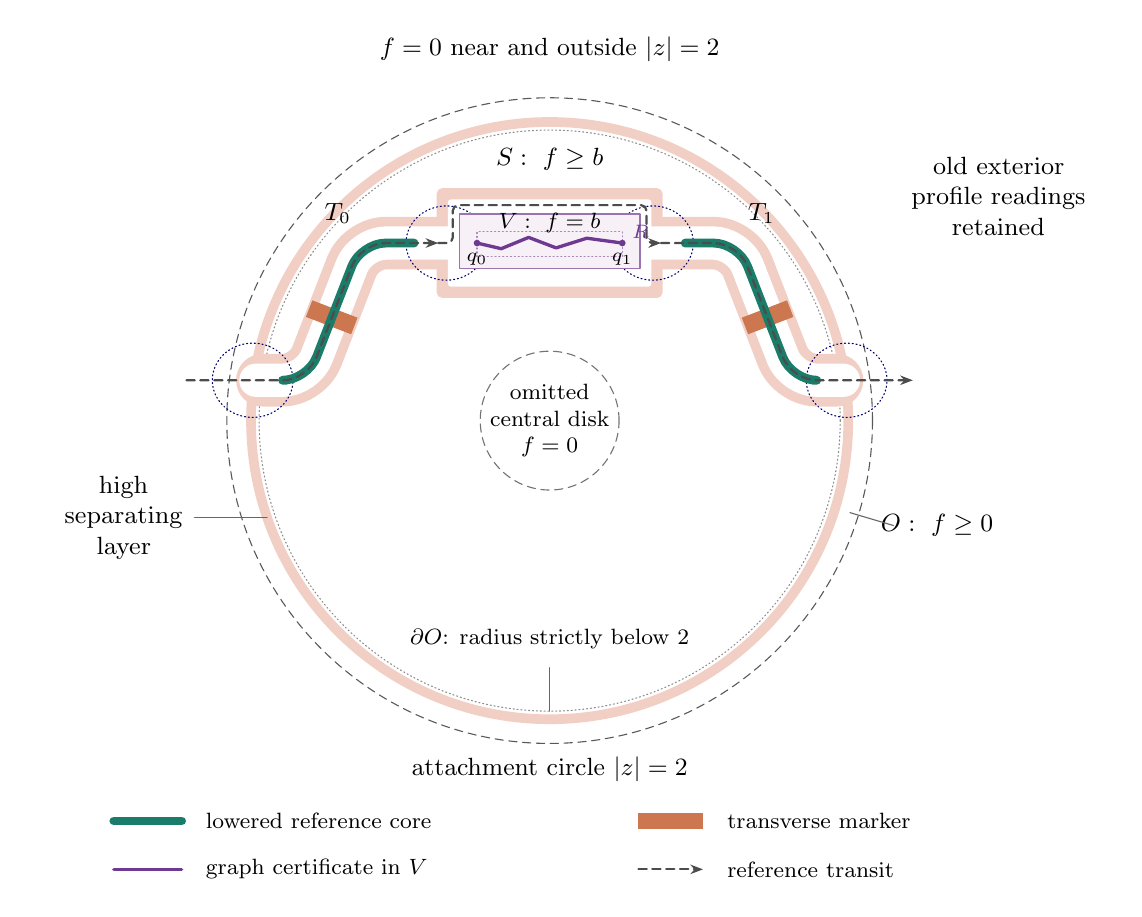
\begin{tikzpicture}[x=2.05cm,y=2.05cm,font=\small,
  line cap=round,line join=round,
  guide/.style={black!60,thin},
  refpath/.style={black!70,densely dashed,thick,
    -{Stealth[length=1.6mm]}},
  shortcutcap/.style={draw=blue!45!black,densely dotted,thin},
  note/.style={align=center,font=\small}]
\definecolor{shortcutwall}{RGB}{241,207,197}
\definecolor{shortcutmarker}{RGB}{204,119,79}
\definecolor{shortcutcore}{RGB}{25,125,105}
\definecolor{shortcutcert}{RGB}{110,57,144}

\draw[black!65,densely dashed] (0,0) circle (2);
\draw[black!45,densely dotted] (0,0) circle (1.80);

\fill[shortcutwall,even odd rule]
  (0,0) circle (1.88) (0,0) circle (1.82);
\draw[shortcutwall,line width=19pt,rounded corners=9pt]
  (-1.78,.25) -- (-1.50,.25) -- (-1.17,1.10) -- (-.57,1.10);
\draw[shortcutwall,line width=19pt,rounded corners=9pt]
  (1.78,.25) -- (1.50,.25) -- (1.17,1.10) -- (.57,1.10);
\fill[shortcutwall,rounded corners=2pt]
  (-.70,.76) rectangle (.70,1.44);
\draw[white,line width=12pt,rounded corners=9pt]
  (-1.82,.25) -- (-1.50,.25) -- (-1.17,1.10) -- (-.57,1.10);
\draw[white,line width=12pt,rounded corners=9pt]
  (1.82,.25) -- (1.50,.25) -- (1.17,1.10) -- (.57,1.10);
\fill[white,rounded corners=1pt]
  (-.63,.83) rectangle (.63,1.37);

\fill[white] (0,0) circle (.43);
\draw[black!55,densely dashed] (0,0) circle (.43);
\node[note,font=\footnotesize] at (0,0)
  {omitted\\central disk\\$f=0$};

\draw[shortcutcap] (-1.84,.25) ellipse [x radius=.25,y radius=.23];
\draw[shortcutcap] (1.84,.25) ellipse [x radius=.25,y radius=.23];
\draw[shortcutcap] (-.64,1.10) ellipse [x radius=.25,y radius=.23];
\draw[shortcutcap] (.64,1.10) ellipse [x radius=.25,y radius=.23];

\begin{scope}[shift={(-1.35,.64)},rotate=69]
  \fill[shortcutmarker] (-.055,-.15) rectangle (.055,.15);
\end{scope}
\begin{scope}[shift={(1.35,.64)},rotate=-69]
  \fill[shortcutmarker] (-.055,-.15) rectangle (.055,.15);
\end{scope}

\draw[shortcutcore,line width=3.2pt,rounded corners=9pt]
  (-1.63,.25) -- (-1.50,.25) -- (-1.17,1.10) -- (-.84,1.10);
\draw[shortcutcore,line width=3.2pt,rounded corners=9pt]
  (1.63,.25) -- (1.50,.25) -- (1.17,1.10) -- (.84,1.10);

\filldraw[fill=violet!6,draw=shortcutcert!70,thin]
  (-.56,.94) rectangle (.56,1.28);
\draw[shortcutcert!60,densely dotted,thin]
  (-.45,1.015) rectangle (.45,1.17);
\node[font=\footnotesize] at (0,1.225) {$V:\ f=b$};
\draw[shortcutcert,very thick]
  (-.45,1.10) -- (-.30,1.065) -- (-.13,1.135)
  -- (.04,1.07) -- (.23,1.13) -- (.45,1.10);
\fill[shortcutcert] (-.45,1.10) circle (1.2pt);
\fill[shortcutcert] (.45,1.10) circle (1.2pt);
\node[below,font=\scriptsize] at (-.45,1.095) {$q_0$};
\node[below,font=\scriptsize] at (.45,1.095) {$q_1$};
\node[right,font=\scriptsize,text=shortcutcert] at (.45,1.17) {$R$};

\draw[refpath,rounded corners=9pt]
  (-2.25,.25) -- (-1.50,.25) -- (-1.17,1.10) -- (-.69,1.10);
\draw[refpath,rounded corners=2pt]
  (-.69,1.10) -- (-.60,1.10) -- (-.60,1.335)
  -- (.60,1.335) -- (.60,1.10) -- (.69,1.10);
\draw[refpath,rounded corners=9pt]
  (.69,1.10) -- (1.17,1.10) -- (1.50,.25) -- (2.25,.25);

\node[above] at (0,1.49) {$S:\ f\ge b$};
\node[above left] at (-1.17,1.16) {$T_0$};
\node[above right] at (1.17,1.16) {$T_1$};
\node[note] at (0,2.30) {$f=0$ near and outside $|z|=2$};
\node[note,text width=2.7cm] at (2.78,1.39)
  {old exterior\\profile readings\\retained};
\node[note] at (2.40,-.65) {$O:\ f\ge0$};
\draw[guide] (2.13,-.65) -- (1.86,-.57);
\node[note,text width=2.2cm] at (-2.64,-.60)
  {high\\separating\\layer};
\draw[guide] (-2.20,-.60) -- (-1.75,-.60);
\node[below] at (0,-2.02) {attachment circle $|z|=2$};
\node[note,font=\footnotesize] at (0,-1.35)
  {$\partial O$: radius strictly below $2$};
\draw[guide] (0,-1.53) -- (0,-1.80);

\draw[shortcutcore,line width=3.2pt] (-2.70,-2.48) -- (-2.28,-2.48);
\node[right,font=\footnotesize] at (-2.19,-2.48) {lowered reference core};
\fill[shortcutmarker] (.55,-2.53) rectangle (.95,-2.43);
\node[right,font=\footnotesize] at (1.04,-2.48) {transverse marker};
\draw[shortcutcert,very thick] (-2.70,-2.78) -- (-2.28,-2.78);
\node[right,font=\footnotesize] at (-2.19,-2.78) {graph certificate in $V$};
\draw[refpath] (.55,-2.78) -- (.95,-2.78);
\node[right,font=\footnotesize] at (1.04,-2.78) {reference transit};
\end{tikzpicture}

\caption{Regions used by one field modification, shown schematically in
outer-shell coordinates. The graph certificate is preserved in \(V\),
where \(f=b\), and old exterior profile readings are preserved beyond
the shell, where \(f=0\). The two disjoint tubes and chamber constrain
reference-metric geodesics: high layers obstruct exits, while lowered
cores and safe cap joins provide access to the terminal caps. The central disk is outside the support.
Shapes and widths represent separation and incidence, not metric distances.}
\label{fig:protected-shortcut}
\end{figure}

\Needspace{6\baselineskip}
Choose a smooth baseline bounded above by a large $H_0$, nonnegative on
$O$, and at least $b$ on $S$. It equals $b$ on the preservation
neighborhood, equals $0$ on the outer safety zones, and equals $b$ on the
terminal safety zones; set it to $H_0$ on the forbidden layer and marker
strips. The clearances just established allow these plateaux. First impose
loose positive old-metric lower cutoffs for crossing the fixed forbidden
gaps and marker strips in $w$ units, and then choose $H_0$ sufficiently
large. A crossing at the unreduced wall or marker height now costs more
than $B_0$.

Subtract $J_0\chi$ from the baseline, where $\chi\ge0$ is smooth and
supported compactly in the smaller tubes, away from the wall layer and
$\overline O\cup\overline S$. In each tube its positivity set is connected
and contains a longitudinal core and its two stops. Choose $J_0$ large.
The following two properties can be imposed by finitely many further
high-probability old-metric cutoffs:
\begin{enumerate}
\item Each core connects its stops at modified cost at most $e$.
\item Every transit from outer to terminal overlap within the tube, or
in the reverse direction, of modified cost at most $B_0$ visits a point
with a modified join of cost at most $2e$ to the corresponding $q_j$,
compactly inside the shell enlargement.
\end{enumerate}
To prove the second property, a transit must meet the core-lowering region
within the marker; otherwise the marker charge exceeds $B_0$. The closure of the possible encounters in a marker is compact.
Choose a finite Euclidean net for it with centers in \(\{\chi>0\}\);
these centers exist because the encounter set lies in that positivity
set. By a further old internal-modulus cutoff, every encounter joins a
net center for cost at most \(e/2\), even at the upper height \(H_0\).
Join the finitely many net centers and stops by paths compactly in the
connected open positivity set. Each chosen path has a positive minimum
of \(\chi\). Impose a deterministic upper cutoff on these finitely
many old lengths and a deterministic positive lower cutoff on these
minima, at arbitrarily small additional probability cost. Then choose
one deterministic finite \(J_0\) making all these connections cheap. No positive lower bound
for \(\chi\) at every possible encounter is needed. Finish with the terminal safe-cap join. This proves the
claim without requiring metric regularity at the exact boundary of a
cheap plateau.

The resulting $f$ is $b$ near the preserved rectangle and is zero near and
outside circle $2$. All amplitudes and cutoff functions, in outer
coordinates, range over fixed finite lists. Coarse-height compensation and
the inner proposals decide only which entries of those lists are useful.
For each recipe also impose a bounded Gaussian change-of-law likelihood
test on its support. Since the list is finite, these tests have
arbitrarily high marginal probability after their cutoffs are enlarged.
They are imposed before any later geodesic event is selected.

Use the conditional kernel comparison of
Lemma~\ref{conf:field-kernel-locality} to
retain the selected certificate from $h+b$ inside the preservation region
and the old profile readings outside a strictly enlarged shell disk in the
modified field $h'=h+f$. The old reference prefixes to $x_j$, safe joins,
cheap cores, and the preserved connection in $V$ give a modified reference
path of length at most
\begin{equation}\label{metric:modified-upper}
 l_0+l_1+B_0<L.
\end{equation}
Here $12e$ accommodates all joining errors in addition to $K_1u$.

Consider a minimizing modified geodesic. It must enter circle $2$ to beat
$L$, since the metric outside that circle is unchanged. Its portion
between first and last visits to the circle has length at most $B_0$:
the unchanged exterior prefixes cost at least $l_0$ and $l_1$.
That portion cannot leave the effective union, because it would cross
the forbidden layer at its unchanged high height and pay more than its
budget. Its first effective tube use from $O$ is on side $0$, and its
last return to $O$ is on side $1$. For if a prefix from $p_0$ in $O$
reached the wrong mouth, it would cost at most $l_0+B_0$; since $f\ge0$
on $O$, the same prefix costs no more in the old field. Complete it by
the old cap join and the old prefix from $x_1$ to $p_1$. This contradicts
\eqref{metric:old-gap}, by \eqref{metric:short-budget}. The reversed
argument handles the last mouth. A transition between the two mouths
through $O$ during the middle portion is excluded by the same local
budget and cap-joining estimate.

Take a finite itinerary subordinate to the effective open cover, switching
only in overlaps. Some excursion from $O$ returns through a different tube
than the departure tube, since remaining in $O$ is impossible and the
first and last types differ. On this excursion choose a transition between
distinct terminal-cap types. This supplies a full approach through one
tube, a full departure through the other, and a portion assigned wholly
to $S$ between opposite terminal caps; spur returns do not alter this
choice. Since $f\ge b$ in $S$, the chamber portion alone costs at least
$d-2e$. The marker accesses on the approach and departure mark an interval
containing it, of length at most $B_0$, whose endpoints have modified joins
of cost at most $2e$ to $q_0,q_1$.

When this geodesic is compactly contained in $U$, the triangle inequality
of Lemma~\ref{metric:certificate-joining}, upper comparison in the modified
law, and the preserved certificate give $F'_U$ cost at most
\[
 c_1d+4Ce
\]
between those interval endpoints. The saving against upper factor $C$
is at least
\[
 C(d-2e)-(c_1d+4Ce)
 \ge \bigl((C-c_1)a'-6Ce_*\bigr)u.
\]
Choose $e_*$ so that the right-hand coefficient is some fixed
$\delta_*>0$ and $d-2e\ge a'u/2$. The chamber portion is inside the
enlarged disk, proving also the stated in-disk length bound. Upper
comparison holds in the modified law by full-field law domination.
Only the reference metric was compared by height inequalities in the
transition regions; the graph certificate was used solely where its
kernel is preserved.
\end{proof}

\subsection{Rigidity by counting modified geodesic visits}

\begin{proposition}[Equality of local comparison factors]\label{metric:rigidity}
In an extraction with diverging denominator units for which upper chaining
gives a finite positive upper optimum $C$, the lower optimum equals $C$.
The common factor is deterministic. This conclusion holds simultaneously
in the fixed-offset experiments with their converted units.
\end{proposition}

\begin{proof}
Suppose $c<C$, and retain the shortcuts, probability tolerances, inner
offset $m$, and finite recipes constructed above. All of these choices are
fixed before choosing the small near-saturation tolerance $\eta$ below.

\smallskip\noindent\emph{A near-saturating compact experiment.}\par
For arbitrarily small $\eta>0$, optimality of $C$ supplies deterministic
ordinary patches $U\Subset W$, a compact protection $K\Subset U$, fixed
anchors $p_0,p_1\in K$, and a positive-probability event $E$ on which
\begin{equation}\label{metric:saturation-event}
 \begin{gathered}
 A<L<A_1,\qquad A>0,\quad A<A_1\le2A,\qquad
 L=D_h(p_0,p_1;W),\\
 \min_{j=0,1}D_h(p_j,W\setminus K;W)>s_0L,\qquad
 F_U(p_0,p_1)>(C-\eta)L,
 \end{gathered}
\end{equation}
where $s_0>1$ has fixed slack. To justify this localization, if there were
no such witnesses, subdivide any reference path and its open following
instructions into sufficiently short subarcs in small ordinary domains
having that exit safety. Compactness, the length topology, and positivity
of exit costs permit arbitrarily fine subdivision in reference length.
Apply the resulting improved $F_U$ bound there, using endpoint continuity
to reduce to countably many anchor tests, and concatenate with
shrinking-cost circuit joins inside the prescribed tubes. This would
improve upper followability strictly below $C$, a contradiction. Restrict
the length to one dyadic window and adjust thresholds slightly to make
them continuity values.

The domains can be kept compactly away from the cylinder ends. The
Brownian-slab comparison of Proposition~\ref{conf:cm-comparison} gives a slab law
retaining positive probability for the witness, with $\overline W$ in
the slab interior, independent $J$, and the same field kernels. Restrict
the end-coordinate parameters only as needed for this room. Refine the
thresholds to continuity values in that law, and write $p_E>0$ for its
probability. Although $E,A,U,W$ may depend on $\eta$, the previously
chosen local recipe constants do not.

The exit safety implies that minimizing paths for these anchors are
attained in $K$, by compactness and the length topology. Such a geodesic
is almost surely unique up to parametrization. Here is an elementary
argument sufficient for these fixed anchors. Distinct geodesics can be
distinguished by a smooth nonnegative bump compactly supported in $W$,
missed by one and visited in its positive set by the other. Under addition
of $t$ times that bump, the distance is nondecreasing in $t$. At a
parameter with these two minimizers it is constant to the right, because
the avoiding minimizer is unchanged, and strictly smaller at every smaller
parameter, because the other minimizer has positive length in the bump's
positive set. There is at most one such parameter for a fixed field and
bump. A countable family of bumps distinguishes all distinct traces.
Local Weyl scaling, Brownian-slab shift equivalence, and Fubini then show
that the exceptional event has probability zero. The whole distance
family is obtained from the original metric by length reweighting, so
this parameter argument uses no additional metric construction or
confluence assertion.

\smallskip\noindent\emph{The input weight of successful visits.}\par
Integrate reference arclength along the middle half of this geodesic on
$E$. The aligned-shell estimate, including the successful shortcut
proposals and all the cutoffs above, gives order $N$ successful holes
around every point, with probability tending to one. For sufficiently
large $N$, the anchors lie outside every visited shell's enlarged disk,
and each disk has room inside $U$. Indeed the middle half is a fixed
positive reference distance from either anchor, while all spatial radii
tend uniformly to zero; use reference continuity, geodesicity, and the
compact safety condition.

Time spent in one hole along the middle half is at most a constant times
its length unit $w$. Replace the portion between first and last encounters
with the attachment circle by a path of cost at most $K_0w$ in its annular
buffer, and use geodesicity. Integrating with multiplicity therefore gives
the expected weight bound
\begin{equation}\label{metric:input-hit-weight}
 \E\!\left[\one_E\sum_{\text{successful hits}}w\right]
 \ge c_0 A p_E N
\end{equation}
for all sufficiently large $N$, with $c_0>0$ independent of $\eta$ and
$E$. Ordinary compact success events whose probabilities tend to one may
be imposed first. Their error is harmless even when $p_E$ is small,
since $E$ and its positive probability are fixed before $N\to\infty$.

\smallskip\noindent\emph{Domination for one transformed hit.}\par
For a successful hit, take a usable recipe from the finite list in
Lemma~\ref{metric:forcing-recipe}. One may count all usable bin and recipe
choices instead of prescribing a choice at an exact endpoint. For each
\emph{fixed} recipe and shell entry, its hit submeasure, together with the
retained inner and old exterior data, is bounded by $\Lambda$ times a
single common output law, where $\Lambda<\infty$ is independent of
$\eta,E,N$.

To prove this domination, first condition on the slab coordinate parameters
and fields, before imposing the hit. Keep the selected independently
proposed inner profile at $h+b$, and the old profile readings beyond a
strictly enlarged comparison disk. The inner preservation region has
$h+f=h+b$; the outer region has $h+f=h$. Source elimination and the
field-kernel comparison give exactly the corresponding two kernels of
the output law at $h'=h+f$. They have the conditional product law, by
\eqref{eq:original-15} after source elimination. Retain jointly all
countable regularized exterior readings with compact confinement in $U$
beyond a strictly containing comparison circle. Each finite collection
is separated from the inner protection and lies in the field-agreement
region, so compact exhaustion gives the whole collection. These kernel
identities hold for typical supported fields, including the deterministic
shifts in the finite list, and are independent of the end and source
choices.

Now apply Cameron--Martin to the fixed shift in the Brownian slab. Its
energy and pairing have the ordinary Dirichlet expression in the local
planar chart: the cylinder coordinate charge is harmonic on the small
support, and the conditional Brownian linear mean contributes no term.
The bounded-likelihood cutoff was part of shell success before selecting
anchors or a hit. Its bound is uniform in the slab endpoints and the
parameters restricted to have the required interior room. Imposing the
hit, choosing a covering bin, or imposing further restrictions only
decreases the resulting submeasure. Complete the output profile over its
retained readings using its usual conditional law; the same domination
then applies to all additional output variables used below. This is a
marginal comparison for one recipe and one entry. It makes no simultaneous
claim about transporting the auxiliary proposals for different entries
to one output realization. Gain and existence requirements can be
expressed by measurable countable tests with slightly weakened slack.

\smallskip\noindent\emph{Stability of the near-saturation event.}\par
The output satisfies the inequalities defining $E$ with errors tending
uniformly to zero over the eligible hits, after a negligible input
restriction if needed. First, anchor distances and exit-safety distances
change by $o(1)$: the shift is bounded and supported in one shrinking
interior ball. Cut a path from its first entrance to its last exit and
splice across that ball. Ordinary continuity of the old internal metric
and the bounded Weyl multiplier control both directions of this
comparison uniformly on an interior compact.

The certificate cost cannot decrease by a nonvanishing amount either.
Suppose an output certificate is cheaper. Mark its first entrance and
last exit on a circle farther out than the transferred-reading threshold,
still with the ball and buffers compactly inside $U$. If the certificate
stays exterior, its reading transfers directly. Otherwise approximate it
with losses tending to zero and extract the two approach points and
subbudgets. Its two exterior pieces have compact confinement exterior to
the threshold and are among the retained readings. The old $F_U$ can
use them and join the two approach points across the ball at cost $o(1)$,
by its triangle inequality and upper bound, together with the uniform
continuity of old internal costs on neighborhoods of the hit region.
Take infima over certificates, using countable intermediate protections
if necessary. Each candidate only needs its own compact confinement in
$U$; no common predetermined distance from $\partial U$ is required.
This proves
\[
 F'_U(p_0,p_1)\ge F_U(p_0,p_1)-o(1).
\]
This argument concerns open endpoint losses, and does not attach an
individual graph vertex to a small ball.

Old modulus and clearance cutoffs make all these errors deterministic
and uniformly vanishing over the shrinking hits, while preserving
\eqref{metric:input-hit-weight}. Hence the relaxed output event has
common-law probability $p_E+o(1)$, by continuity of the thresholds. Its
safety still gives minimizing paths in $K$ for large $N$.

\proofstage{A bound on the total output weight}
For each eligible transformed hit, the unique output geodesic has the
strict-gain interval and the in-disk traversal supplied by
Lemma~\ref{metric:forcing-recipe}. The per-label overlap tests of the
aligned-shell construction are unchanged by this one shift: its own
large outer circle average, the required neighbor averages, and the
coarser delay checks are all outside the support. Thus eligibility can
be defined using only necessary output properties: these unchanged
alignment tests, the relaxed event, and existence of the weakened gain
and traversal requirements. On every realization of the common output
law, eligible enlarged disks have bounded overlap for each label,
including the fixed finite recipe multiplicity.

Their marked intervals also have bounded overlap in geodesic time for
each label. All intervals containing a specified time lie in a span of
length at most $2B_0$, since each has length at most $B_0$. Each spends
at least \(a'u/2\) in its own enlarged disk. If the disks have overlap
at most \(M\) at this label and \(n_t\) intervals contain a given
time \(t\), summing these in-disk durations gives
\[
 n_t\,\frac{a'u}{2}\le 2M B_0,
 \qquad n_t\le\frac{4M B_0}{a'u}.
\]
The right-hand side is fixed because \(B_0/u\) is fixed. Partition the intervals into a bounded number of
families of disjoint intervals. Within a family, use the triangle
inequality for $F'_U$ to splice the improved pieces with the intervening
geodesic portions, charged at upper factor $C$. The total gain satisfies
\[
 \sum\delta_*u\le C L'-F'_U(p_0,p_1)
 \le O(\eta A)+o(1),
\]
where $L'=D_{h'}(p_0,p_1;W)$. The geodesic is compactly in $K\Subset U$,
so its subpaths are admissible for every such splice. Since
$w=2^{\xi m}u$ and $m$ is fixed, summing the bounded number of families,
then the labels in $[N,2N]$, gives
\begin{equation}\label{metric:output-hit-weight}
 \sum_{\text{eligible output hits}}w\le C_2\eta A N
\end{equation}
on the relaxed event, for all sufficiently large $N$. Here $C_2$ is
independent of $\eta,E,p_E$. Countable interval tests and slightly weaker
gains can be used throughout to make this bound measurable.

Apply the per-hit domination and integrate
\eqref{metric:output-hit-weight}. Together with
\eqref{metric:input-hit-weight} it yields
\[
 c_0A p_E N\le \Lambda C_2\eta A\bigl(p_E+o(1)\bigr)N.
\]
Choose $\eta>0$ sufficiently small first, obtaining its fixed event of
probability $p_E>0$, and then take $N$ sufficiently large. This is a
contradiction. Thus $c=C$, as claimed.
\end{proof}

\subsection{Quantile comparison and the scale bootstrap}

\begin{lemma}[Quantiles in a rigid extraction]\label{metric:rigid-quantiles}
For the rigid extractions of Proposition~\ref{metric:rigidity}, there
are deterministic constants $0<d_0<D_0<\infty$, independent of the
extraction and of each fixed integer offset $r$, such that
\begin{equation}\label{eq:original-17}
 d_0C\le\liminf\frac{A_{j-r}}{Tw_r}
 \le\limsup\frac{A_{j-r}}{Tw_r}\le D_0C.
\end{equation}
This includes forward offsets. In extractions with $T=A_j$ the common
factor $C$ lies in a universal compact subinterval of $(0,\infty)$.
There is also a fixed sufficiently small $d_1>0$ such that the lower
traversal test at threshold $d_1A_{j-r}$ strictly re-passes in these
extractions, with the required band slack.
\end{lemma}

\begin{proof}
Use the transported prototype law at offset $r$. Upper following of
finitely many reference winding instructions with strict clearance and
forced transverse stitching gives an upper probability cutoff for the
circuit cost at a fixed multiple of $C$. Lower comparison charges a
nontrivial compact subtraversal of every winding path, giving a strictly
positive lower probability cutoff at a fixed multiple of $C$. The
reference lengths in question have the same finite upper and positive
lower probability cutoffs at every offset. Together with the two
quantile inequalities \eqref{metric:quantile-tests}, these bounds give
\eqref{eq:original-17}. All margins are taken strict before returning
to the measurement band.

At a quantile-normalized label with finite upper comparison, the second
inequality in \eqref{metric:quantile-tests} already forces $C>0$ by
upper following, so Proposition~\ref{metric:rigidity} applies.
Putting $r=0$ and $T=A_j$ in \eqref{eq:original-17} gives
$1/D_0\le C\le1/d_0$. Finally, lower comparison by $C$ and the common
positive reference traversal cutoff give high-probability lower
success at a fixed small multiple of $CTw_r$. The upper bound in
\eqref{eq:original-17} makes $d_1A_{j-r}$ strictly smaller than this
threshold for sufficiently small fixed $d_1$. This gives the last
assertion with its probability and geometric slack.
\end{proof}

\begin{proposition}[Deterministic scale and local comparison]\label{metric:scale-bootstrap}
Define
\[
 \mathcal B(P)=A_{\lfloor\log_2P\rfloor}
\]
for large $P$, extending it positively for small $P$. For every
$\sigma\in(0,\xi)$ there is a finite deterministic $K_\sigma$ such that
\begin{equation}\label{eq:original-18}
 \frac{\mathcal B(P')}{\mathcal B(P)}
 \le K_\sigma\left(\frac{P'}P\right)^\sigma,
 \qquad 1\le P'\le P.
\end{equation}
Along every sequence of diverging perimeter units there is a further
joint extraction on which the lower and upper open-port comparison
factors in denominator units $\mathcal B(P)$ agree. Their common value
is deterministic and lies in a universal compact positive range.
These local almost-sure comparisons also hold on ordinary patches of
the unit-area sphere.
\end{proposition}

\begin{proof}
Fix $\sigma\in(0,\xi)$. At every sufficiently large index test the
following three assertions:
\begin{enumerate}
\item $M^{-1}<A_j/A_{j-1}<M$, for a fixed large $M$;
\item $A_{j-m_0}/A_j<2^{-\sigma m_0}$, for a fixed large integer $m_0$;
\item lower traversal success at threshold $d_1A_j$.
\end{enumerate}
Choose these constants so that rigid comparisons strictly re-pass all
three tests. Such a choice is possible by
Lemma~\ref{metric:rigid-quantiles}. In particular, choose $M$ larger
than the uniform bounds for the adjacent ratios. Then take $m_0$ so
large that the fixed multiplicative loss in
\eqref{eq:original-17}, times $2^{-\xi m_0}$, is strictly smaller
than $2^{-\sigma m_0}$. The lower test uses the fixed $d_1$ of that
lemma, decreased if necessary to retain strict slack.

Every fixed finite success run eventually holds about the record starts
of Lemma~\ref{metric:records}. Indeed, every extraction at such starts
has the upper ratio bound \eqref{metric:record-ratios} at all fixed
preceding offsets. Upper chaining gives a finite upper constant, and
quantile normalization makes it positive. Proposition~\ref{metric:rigidity}
and Equation~\eqref{eq:original-17} then apply at all fixed offsets,
including forward ones. A failure in a fixed finite run would contradict
their strict retests after further joint extraction.

Suppose nevertheless that there are later first exits after arbitrarily
long successful runs. Extract at the index $j$ immediately before such
a first failure. All fixed backward offsets, including zero, now pass
the three tests. The adjacent bounds permit a further extraction with
\begin{equation}\label{metric:ratio-sequence}
 r_i=\lim\frac{A_{j-i}}{A_jw_i}\in(0,\infty)
 \quad(i\ge0),\qquad r_0=1.
\end{equation}
We claim that these $r_i$ are uniformly comparable.

Fix a starting offset $i$. In $A_jw_i$ units, the farther tests at relative
offset $l$ give high upper and lower factors of order $r_{i+l}$ in
their exact-power units. If at least a fraction $1/10$ of the offsets
$l\in[N,2N]$ had $r_{i+l}\ge L_0r_i$ along arbitrarily large $N$,
lower chaining would give a lower factor of order $L_0r_i$ at $i$.
For a sufficiently large absolute $L_0$, this contradicts the winding
upper test there, whose scale is $r_i$. If instead the same fraction
had $r_{i+l}\le r_i/L_0$, upper chaining would give an upper factor
of order $r_i/L_0$, contradicting the second quantile inequality at $i$.
The chain constants and reference probability cutoffs are uniform, as
proved above. Thus, for each fixed $i$, a large majority of all
sufficiently long such intervals satisfy
\[
 r_i/L_0<r_{i+l}<L_0r_i.
\]
The large-majority sets for any two fixed starting indices overlap
after translating their intervals by the bounded difference of these
indices. A common member shows that their $r_i$'s differ by at most
$L_0^2$. Comparing with $r_0=1$ proves the claim.

At the index before failure, \eqref{metric:ratio-sequence} now gives an
upper ratio bound by a fixed multiple of $w_i$ at every fixed preceding
offset. Upper chaining again gives finite upper comparison; normalization
gives positivity; and rigidity follows. Equation~\eqref{eq:original-17}
and its lower traversal retest strictly re-pass all the tests at the
alleged failure index, a fixed forward offset. This is a contradiction.
Consequently all three tests hold eventually.

The same majority argument applies to any extraction at later indices:
the adjacent tests give positive finite fixed-offset limits, the upper
and lower tests make them uniformly comparable, and chaining followed
by rigidity gives equality of the comparison factors in $A_j$ units.
Lemma~\ref{metric:rigid-quantiles} bounds these factors uniformly above
and away from zero.

Iterate the second eventual test in blocks of length $m_0$ and use
the adjacent test for the fewer than $m_0$ remaining steps. After
enlarging a deterministic constant to include the finitely many small
indices, this gives
\[
 \frac{A_{j'}}{A_j}\le K\,2^{-\sigma(j-j')},\qquad j'\le j.
\]
Converting dyadic indices to $P',P$ costs only a fixed factor and proves
\eqref{eq:original-18}. In particular $\mathcal B(P)\to\infty$.

For arbitrary diverging perimeter units, their ratio to the lower
dyadic unit lies in $[1,2)$. Pass to a subsequence where it has a
positive limiting ratio, and apply the joint fixed-ratio unit conversion
of Lemma~\ref{kern:unit-conversion}. This transfers the same local statements,
with a deterministic common factor in a universal compact positive
range, after further extraction. Only local internal reference length
data occur in these assertions. The fixed-volume product rule
\eqref{eq:original-15}, retained by Proposition~\ref{kern:fixed-volume},
and the field matching and area-one transfer of
Lemmas~\ref{conf:field-kernel-locality} and~\ref{kern:area-one-transfer}
therefore transport them to ordinary patches of the unit-area sphere.
\end{proof}

\begin{remark}[Scope of the local conclusion]\label{metric:no-endpoint-control}
The upper statement follows complete finite-length reference paths with
arbitrary open loss. The lower statement applies to \emph{all} compactly
confined bounded-cost graph paths, and its positive factor also bounds
intrinsic reference distance in an open collar. Neither statement gives
a diameter bound for all vertices approaching a point, or the cost of
attaching an arbitrarily specified lattice endpoint. These additional
estimates are proved in Sections~\ref{sec:endpoints} and~\ref{sec:address}.
\end{remark}

\section{Balanced segments and continuity at all endpoints}\label{sec:endpoints}
The local comparisons of Section~\ref{sec:metric} identify the metric away from the
excluded points and give the deterministic scale estimates
\eqref{eq:original-18}. We now control endpoints uniformly. The proof first reduces
the problem to an estimate for bad times in balanced explorations. We then prove
the passage statement that enters the address count of Section~\ref{sec:address}.
All graph lengths below count every original primal edge, with its original unit
length; auxiliary Tutte paths serve only to locate the necessary primal joins.

\subsection{Balanced segments and the volume spine}

\begin{lemma}[A strict exponent margin]\label{end:exponent}
The critical metric exponent satisfies $\xi>1/4$.
\end{lemma}

\begin{proof}

We use the critical exponent characterization in the Ding--Gwynne LFPP results
\cite[Section~1.2, Equations~(1.4)--(1.7)]{DGuniqueness} (whole-plane pinned GFF, heat regularization at length \(\epsilon\),
median internal square crossing \(\epsilon^{1-2\xi+o(1)}\)). Indeed for any
\(\sqrt2<t<2\), all but \(o(\epsilon^{-1})\) of the \(\epsilon\)-squares in that square
have regularized field everywhere at least \(-t\log(1/\epsilon)\), in the sense that the
\textbf{number of exceptions} is \(o(\epsilon^{-1})\) in probability. This is by Gaussian
tails and first moment (use an intermediate exponent); unit-\(\epsilon\)-box field
oscillations have uniformly Gaussian supremum tails by the heat-kernel covariance
derivative bounds after scaling (center variance \(\log(1/\epsilon)+O(1)\)). Hence order
one of projected crossing length must use this lower height, giving \(1-2\xi\le t\xi\).

Since $t<2$, the inequality gives $\xi\ge 1/(2+t)>1/4$.

\end{proof}

\begin{definition}[Balanced segment]\label{end:balanced-segment}

In a Boltzmann disk $T_p$, start at a specified active edge without
choosing a target. At a face step choose the side fairly. At a bridge,
detach the smaller disk and retain the larger, with a fixed convention on
ties. Update the active edge to the nearest slot beyond it on the chosen
side, according to the two-list rule of Section~\ref{sec:cutting}.
Stop after
\[
 T=\max(1,\lfloor m_p\rfloor)
\]
steps, or on the first exit of the perimeter from $[p/2,2p]$.
For bounded positive $p$, choose $T$ bounded and take at least one step.
The segment children are all detached disks, including ring interiors,
and the final unexamined disk. Recurse in every child of positive perimeter;
a zero-perimeter singleton needs no segment.

\end{definition}

\begin{lemma}[Access to ancestral tip trajectories]\label{end:tip-access}
The balanced recursion exhausts the disk. Its active-edge midpoints can be
joined into tip trajectories $\gamma_p$ using boundedly many Tutte edge
portions per step. Every site can reach its ancestral tip trajectories by
following the recursion, with bounded local Tutte cost at each transition,
apart from travel along those trajectories.
\end{lemma}

\begin{proof}
Consecutive active edges have common or adjoining tip vertices: the nearest
retained slot shares the corresponding endpoint, and a bridge joins the
retained and detached endpoints. These incidences join successive active
midpoints, including the final absorption, at bounded Tutte cost.
For a ring child, start at the corresponding first inner base. It is
reachable by boundedly many Tutte links, since consecutive outer bases with
no intervening inner run adjoin the same inner vertex. Choose the root of
each recursive child at this transition site.

Every exposed site lies on a tip trajectory, on an adjoining ring or child
boundary, or in a singleton attachment. A site not yet exposed remains in
one of the children with its boundary occurrences retained. Iterating these
alternatives gives the asserted access to the ancestral trajectories.
The finite recursion exhausts the map by the exact peeling decomposition
\eqref{eq:original-5}.
\end{proof}

\begin{lemma}[Stopped word law]\label{end:segment-law}
For sufficiently large $p$, the complete word of a balanced segment in $T_p$ is dominated by a fixed constant times the raw iid word experiment of \eqref{eq:original-12}, with the same deterministic time bound and perimeter stopping rule. Conditional on the word, its unexamined fillings have the marked product laws.
\end{lemma}

\begin{proof}

Before stopping, the word of signed two-coordinate increments uses \eqref{eq:original-12},
with negative magnitude restricted to keeping the larger (\(j\le(S-2)/2\)) and the tie
factor, and overall likelihood \(f_{S_{\rm stop}}/f_p\); overshoot down is no smaller than
\((S-2)/2\), overshoot up unrestricted. In particular this whole stopped segment word for
large \(p\) is boundedly dominated by the raw iid experiment to time \(T\) with the same
stopping (invalid negative steps need not be used). Fillings are conditionally the marked
products as before.

The bound is uniform in the stopped word. Before exit, the perimeter is
comparable to $p$. A downward exit keeps at least $(S-2)/2$ and hence at least
a fixed positive multiple of $p$; an upward exit can be arbitrarily large, but
the perimeter weight decreases at the polynomial rate already established.
The ratio $f_{S_{\rm stop}}/f_p$ is therefore bounded in both cases. The
restriction on negative jumps and the tie convention can only remove raw words
or decrease their multiplicity.

\end{proof}

\begin{lemma}[Volume weights and logarithmic spine moments]\label{end:volume-spine}
Let $V(p)=\E N_p$. Then
\[
 V(p)\sim\frac{c_*^2}{4f_p}\asymp\frac{p^2}{\log p},\qquad p\longrightarrow\infty,
\]
with $V(p)>0$ for $p>0$ and $V(0)=0$. For the segment-child kernel
\[
 \mathcal K(p,q)=\frac{V(q)}{V(p)}
 \E\#\{\text{children of perimeter }q\},\qquad p,q>0,
\]
volume additivity makes $\mathcal K$ substochastic. As $p\to\infty$, its mass tends
to one, its logarithmic ratio drift tends to zero, its logarithmic ratio second
moment stays bounded above and below by positive constants, and its logarithmic
ratios have uniformly bounded two-sided exponential moments of sufficiently
small order.
\end{lemma}

\begin{proof}

In \eqref{eq:original-6} the perimeter moment's \(c\)-derivative equals \[
 p F_{p-1}+\tfrac14\,\mathbb E[(c-U)^p(U-\eta/U)]
\] by the differentiation above. At \(c\downarrow c_*\) the \(\eta/U\) term is bias
converging to an atom of mass \(c_*\) at zero (\(\eta=c/m_{-1}\)). Consequently the
derivative divided by \(c_*^p\), after this limit then \(p\to\infty\), tends to \(-c_*/4\)
(the other terms vanish by the moment equivalent and the endpoint gap). Thus
\(V(p)\sim c_*^2/(4 f_p)\asymp p^2/\log p\), finite positive for \(p>0\), zero for
\(p=0\).

Use the substochastic spine kernel on positive perimeters \[
             {\cal K}(p,q)=\frac{V(q)}{V(p)}
                    \mathbb E\,\#\{\text{segment children of size }q\},
\] using volume additivity/domination. Its large-\(p\) masses tend to one, log ratio drift
to zero, variance stays between positive constants, with uniformly bounded two-sided small
exponential moments of log ratio. Here is the stopped-segment calculation. Let $\tau$ be the stopping
step, $S_r$ the retained perimeter just before step $r$, and $Q_r$ the
perimeter of the child detached at that step (the inner perimeter at a
ring step). The final retained disk is itself a child. For $z$ near $2$,
with $0^z=0$, the exact telescoping identity is
\[
 \E\sum_{q\text{ child}}(q/p)^z-1
 =\E\sum_{r<\tau}p^{-z}
       \bigl(S_{r+1}^{\,z}+Q_r^{\,z}-S_r^{\,z}\bigr).
\]
The first and second derivatives in $z$ give the corresponding
logarithmic-ratio moments. We estimate the one-step summands before
summing them over the stopped path. For one step from
\(s\to\infty\), the scaled drift (including the detached child) of perimeter power \(z\)
relative to \(s^z\), times \(m_s\), tends near \(z=2\), with first two derivatives, to \[
       G(z)=\mathrm{PV}\int_{-1/2}^{\infty}
       \frac{(1+v)^z-1+|v|^z}{(1+v)^2}\frac{dv}{v^2}.
\] Indeed use the \eqref{eq:original-12} equivalents, \(f_{s+d}/f_s\) likelihood, and the
positive-face inner/outer ratio tending to one with geometric-run and smooth tilt tail
bounds. Truncated signed first moment of the unrestricted raw increments is bounded; at
small \(|d|/s\) use \(|f_{s+d}/f_s-1|\le C|d|/s\), second-order cancellation for the
survivor term and absolute power integrability for the detached term. For the latter all
positive outer sizes \(k\) have inner powers up to slightly past 2 bounded in expectation
by \(C(1+k)^z\) from the geometric sum tilt; use nearby powers also for log factors. At
the upper tail the additional likelihood decays as at least power \(2-\delta\); these
bounds give dominated truncations. 

For the small-step likelihood bound used here one may
take the limiting positive moment law from \eqref{eq:original-6}, normalized in \(c_*\)
units, whose negative endpoint has modulus \(<1\). On \(y\in[0,1]\),
\(|y^{s+d}-y^s|\le C (|d|/s)y^{s/4}\) for \(|d|\le s/2\); moments there at comparable
indices are bounded by \(O(f_s)\) by the equivalent and the exponentially small
negative-cut contribution. The latter itself causes no problem for nonzero integer \(d\).
The two coordinates together have the stated unit Lévy coefficient. 

Now \(G(2)=0\) by
integrating \(2/[v(1+v)]\). For \(G'(2)\) the first integral
\(\mathrm{PV}\int \log(1+v)dv/v^2=2\log2\); the second is
\(\int \log|v|\,dv/(1+v)^2=-2\log2\) by substituting \(v/(1+v)\). Also \(G''(2)>0\). 

Sum
these drift estimates over pre-stopping states (all comparable to \(p\)), multiplying by
\((s/p)^z\) and including derivative terms; expected step count divided by \(m_p\) is
bounded and bounded below (a small initial time with small raw oscillation has positive
probability by Cauchy convergence and the bounded positive likelihood there). This gives
the claimed weighted estimates first with \((q/p)^2\) weights. Replacing by \(V(q)/V(p)\)
is harmless by the nearby power bounds and the equivalent. Indeed the ratio is comparable
on compact positive ratio ranges and controlled off them by arbitrarily small
positive/negative power losses relative to \((q/p)^2\) from the
\(\asymp (1+p)^2/\log(2+p)\) estimates on positive perimeters, with relative multiplier
tending to one on the compact ranges.

\end{proof}

\begin{proposition}[Simultaneous segment counts]\label{end:band-counts}
Start a balanced recursion at $p_{\rm init}\asymp B_n$ and stop a branch when it
first exceeds $p_*=C_*B_n$. The probability of any such crossing tends to zero
as $C_*\to\infty$. For every $\delta_1>0$, sufficiently small, the expected
number of nodes with $k=\lfloor\log(p_*/p)\rfloor$ is at most
$C e^{(2+\delta_1)k}$. With arbitrarily high probability, simultaneously for all
ancestry lines and all $k\ge0$, the number of such nodes on any one line is at
most $C e^{\delta_1k}$, with a suitable deterministic $C$.
\end{proposition}

\begin{proof}

Start at \(p_{\rm init}\asymp B_n\) and truncate on rising above \(p_*=C_* B_n\), which
somewhere in the tree has probability bounded by \(V(p_{\rm init})/\inf_{p>p_*}V(p)\) by
the spine/first-hit sum; \(C_*\) can be chosen large. Put
\(k=\lfloor\log(p_*/p)\rfloor\ge0\) for bands. For each small \(\delta_1>0\) the expected
number of nodes in band \(k\) before such crossings is \(\le C\exp((2+\delta_1)k)\).
Moreover with arbitrarily high probability, simultaneously over all ancestry lines and
\(k\), at most \(C\exp(\delta_1 k)\) such nodes occur per line. To see it on the
killed/upper-stopped spine, tilt steps at large \(p\) by \(e^{\theta\log(q/p)}\) and
normalize for fixed sufficiently small \(\theta>0\). Normalizers then exceed one, tilted
drift is bounded below positively, and a small negative exponential of the increment has
tilted expectation \(<1\), uniformly beyond a fixed cutoff, by the preceding moment
bounds. From a band visit sufficiently high above that cutoff, with uniformly positive
tilted probability the chain stays above cutoff and crosses the upper barrier in
\(O_\theta(k+1)\) steps with log total rise \(\le C_0(k+1)\) at crossing (absolute
coefficient for large \(k\)). Indeed use the negative-exponential supermartingale for
avoiding cutoff, the positive drift and bounded variances, and the step tail for the
overshoot. Thus before tilting a kill/crossing within that many steps still has
probability at least \(c_\theta e^{-C_0\theta k}\). On the remaining fixed bounded
perimeters there is uniform direct kill probability (positive expected exposed ring
volume). Let $N_k$ be the number of visits to band $k$ by this killed,
upper-stopped spine. Restarting at later visits gives
\[
 \Prob_{\rm spine}(N_k\ge m)
 \le \exp\!\left[-q_k
          \left\lfloor\frac{m}{C_\theta(k+1)}\right\rfloor\right],
 \qquad q_k\ge c_\theta e^{-C_0\theta k}.
\]
The volume bias converts this to both asserted tree estimates. Indeed,
\[
 \E\sum_{v:\,p_v\text{ in band }k}
          \frac{V(p_v)}{V(p_{\rm init})}
       =\E_{\rm spine}N_k.
\]
On this band, $V(p_{\rm init})/V(p_v)\le Ce^{2k}$.
The same identity at the stopping line of the $m$th band visit gives
\[
 \Prob\{\text{some ancestry line has at least }m\text{ band visits}\}
 \le Ce^{2k}\Prob_{\rm spine}(N_k\ge m).
\]
Choose $\theta$ so small that $C_0\theta<\delta_1$ with strict slack.
Summing the geometric tail proves the expected-node bound. Substituting
$m=Ce^{\delta_1 k}$ and then summing over $k$ proves the simultaneous
ancestry bound, with arbitrarily high probability as $C$ increases.
Fresh
disk tests at a node can then use its unconditional \(T_p\) probabilities.

\end{proof}

\begin{lemma}[Transfer and local incidence costs]\label{end:finite-sphere-transfer}
The preceding recursion estimates apply, with bounded domination, to both
initial disks in a restricted central comparison with the unit finite sphere.
Under the rooted sphere law, the maximum vertex degree and maximum face degree
are $O(\log n)$ with probability tending to one. On this event a bounded local
Tutte advance or incidence join can be replaced by a primal join of cost
$O(\log n)$.
\end{lemma}

\begin{proof}

Both initial disks of the restricted central comparison obey these bounds with bounded
domination in the unit finite sphere: leave the opposite disk for volume smoothing by
\eqref{eq:original-10}, localizing both initial perimeters in positive compact ranges.
Also the full sphere has vertex and face degrees \(O(\log n)\) with probability tending to
one under the rooted law. Indeed at a vertex of root degree \(d\) split its list from the
root into \(j+1\) nonempty consecutive groups in order, replacing the vertex by a path
with \(j\) occupied connecting edges and placing the groups along one flank at the
successive vertices with the other flank free. Given \(j\) invert by tracing that empty
flank starting adjacent to the root half-edge in the specified rotation and contracting;
the FK exponent is unchanged. Thus a root-origin degree tail costs at most
\(Z_{n+j}/(Z_n\binom{d-1}{j})\); use \eqref{eq:original-3} and \(j\) a sufficiently small
fixed fraction of the threshold for exponential decay. Use duality and uniform rerooting.
This high-probability bound may be intersected \textbf{after} transferring estimates back
from central intensity by dividing by counts.

On the degree event, incident primal vertices around a face have primal
joining distance $O(\log n)$. Within a disk we use genuine primal edge portions,
including the possible blue half-diagonals up to a boundary red base; the costs
of these internal primal walks carry to the joined sphere.

\end{proof}

\subsection{The bad-time estimate and the endpoint reduction}

We give the reduction to a one-segment estimate, stated explicitly to separate the
endpoint issue. Choose \[
 1/4<\tau<\varrho<s<\sigma<\min(\xi,1).
\] Use \eqref{eq:original-18} with \(\sigma\). Take \(b>1\) sufficiently close to 1
(\(s-(b-1)>\varrho\)), then \(a>1\) much closer to 1 with \(a<b\). A small truncation
constant \(\delta>0\) can first be chosen so that \(\sigma-\varrho\gg\delta\), then
\(b-1\ll\delta\). Consider diverging perimeter parameters \(p_*,p\), put
\(k=\lfloor\log(p_*/p)\rfloor\), and take integer \(N\to\infty\) with \(k\le C N,\ k+N\le(1-\delta)\log p_*\). Time sizes will be
\(T e^{-x}\). In each time interval of size \(T e^{-N}\) test grid times at spacing
\(T e^{-bN}\) (integer rounding permitted). Only test times of the executed path outside
endpoint strips of width \(O(T e^{-aN})\) at start and stop.

\begin{definition}[Good grid time]\label{end:good-time}

A good time has a simple short separating boundary, either a primal circuit in the
disk or a simple primal crosspath capped in the external root face. Its real portion costs
at most \(\mathcal B(p_*) e^{-s(k+N)}\) up to harmless bounded factors. One open side
contains the path throughout a time neighborhood of radius at least the grid spacing
(rounding with slack); both full-segment ends are strictly outside, and the component time
interval in that side about the tested time ends on both sides within \(T e^{-aN}\) up to
fixed factors. Shifted constants/finer intermediate ranges with slack are harmless.

\end{definition}

\begin{proposition}[Bad grid times]\label{end:bad-grid}

For each prescribed \(B,C\), with failure probability \(O(e^{-B N})\) under \(T_p\),
\textbf{every} such base interval (intersect the executed path) has at most
\(\exp(\tau(b-1)N)\) bad grid times, outside the stated strips. It suffices to use a mesh
of base intervals and allow a constant multiple of this bound on arbitrary intervals. In
this reduction and the estimate one can spend strict exponent slack in all the displayed
inequalities.

\end{proposition}

Proposition~\ref{end:bad-grid} is proved in Section~\ref{sec:address}. The
remainder of this section prepares its passage input. Before doing so, we show
exactly how that proposition completes the missing endpoint control.

\begin{proposition}[Uniform endpoint continuity]\label{end:endpoint-reduction}
Assume Proposition~\ref{end:bad-grid}. For every $\varepsilon>0$,
\[
 \lim_{r\downarrow0}\limsup_{n\to\infty}
 \Prob\left[
 \sup_{\substack{u,v\in V(M_n)\\\rho(\phi_n(u),\phi_n(v))\le r}}
 \frac{d_n(u,v)}{\mathcal B(B_n)}>\varepsilon
 \right]=0.
\]
Normalized diameters are tight. Every subsequential limit of the entire embedded
distance graph equals the same deterministic multiple of $D_h$ already
identified by the local open-port comparisons, including at the excluded points.
\end{proposition}

\begin{proof}

\smallskip
\noindent\textbf{Intersecting good intervals and the recurrence.}\quad

Indeed overlapping good component intervals with neither contained in the other have
intersecting real boundary paths. For two capped paths, if cap endpoints alternate, the
real paths already have to meet by planar order (the root face gives the occurrence order
even when the boundary is pinched); otherwise one can cap disjointly when testing that
pair. Coincident real endpoints already give contact. Nonintersecting boundaries would
then be nested if their open chosen sides overlap, since both avoid the common start point
also in their closures, and the overlapping component intervals would nest. Internal
capped/full contacts suffice anywhere on the real portions. Thus one can prune
containments in each intersecting chain and join along actual paths paying at most their
total real lengths and the local incidence corrections. The endpoints at uncovered gaps
are actual hits on those paths. Uncovered gaps across a tested interval require in sum
\(O(1+\#\mathrm{bad})\) intervals of size \(O(T e^{-bN})\), since every non-end good grid
time covers a spacing on both sides. More explicitly gaps of even shorter length must have
separating bad centers between the good centers of their two chains. Endpoint remainders
caused by using intersecting intervals, or by skipping the two full-segment end strips,
cost only \(O(1)\) intervals of size \(O(T e^{-aN})\).

Consequently if \(\Omega(N)\) bounds joining costs for tip-point pairs within \(T e^{-N}\)
(using adjoining blue representatives in the joined sphere), it suffices recursively to
pay
\[
 \begin{aligned}
 &O(1)\Omega(\lfloor aN\rfloor)
   +O(e^{\tau(b-1)N})\Omega(\lfloor bN\rfloor)\\
 &\qquad+O(e^{(b-1)N})
       \bigl[\mathcal B(p_*)e^{-s(k+N)}+O(\log n)\bigr].
 \end{aligned}
\]
The second line accounts for circuits, capped paths, and incidence
transitions. Fixed size factors can instead shift log indices by bounded amounts. Start
this on all integer levels \(N\ge\max(M_0,c_2 k)\) with small \(c_2>0\), stopping
recursion at \(k+N\ge(1-\delta)\log p_*\). In the terminal range reached from below
(\(k+N\le(1-\delta/2)\log p_*\) after choices), trivial chronological costs
\(O((1+T e^{-N})\log n)\) are negligible relative to \(\mathcal B(p_*)e^{-\varrho(k+N)}\).
For completeness, divide each recursive term by the proposed bound
\(Q(N)=\mathcal B(p_*)e^{-\varrho(k+N)}\). Apart from bounded shifts of the indices,
the two recursive coefficients are bounded by
\[
 C e^{-\varrho(a-1)N}
 \quad\text{and}\quad
 C e^{-(\varrho-\tau)(b-1)N},
\]
and the circuit-cost ratio is at most
\[
 C e^{-(s-\varrho)k-[s-\varrho-(b-1)]N}.
\]
Each tends to zero by the strict exponent choices. The incidence errors are
absorbed by \(b-1\ll\delta\ll\sigma-\varrho\). At the terminal levels the
chronological time is at most a constant times \(p_*^\delta\), up to logarithmic
factors, whereas \eqref{eq:original-18} makes the proposed bound a larger
positive power of \(p_*\); the same margin absorbs the terminal \(\log n\) costs.
Choose \(M_0\) so that the sum of the recursive coefficients is less than one,
and use the negligible terminal costs to initialize downward induction. This
gives the bound \(Q(N)\) throughout the recursion. Bands starting
already too small need only trivial whole-trunk costs, \(\ll\mathcal B(p_*)e^{-\eta_0 k}\)
for some \(\eta_0>0\) by taking \(c_2,\delta\) small. Summing starting-mesh intervals on a
trunk similarly yields \(\ll_{M_0}\mathcal B(p_*)e^{-\eta_0 k}\), as well as normalized
chronological equicontinuity on bounded \(k\). By the spine bounds and fresh-disk
estimates with \(B\) large, \(M_0\) can give arbitrarily high joint success probability
over nodes and levels. Sum along each ancestry using \(\delta_1\ll\eta_0\), also absorbing
\(O(\log n)\) attachment errors per node. This implies uniform approximation of vertices,
at normalized cost error tending to zero with band cutoff, by points on the finitely many
macroscopic tip trajectories (use the last sufficiently large ancestor). Central ring
sites are covered on the initial disks. In these high-probability arguments
\(\mathcal B(p_*)/\mathcal B(B_n)\) is bounded for fixed truncation by the adjacent-ratio
bounds. One may first spend an arbitrarily small \textbf{fixed} probability error on the
perimeter/degree truncations and the constants in the visit and trunk bounds, then test a
putative failure in a further coupled limit on the remaining events (with bounded-band
node counts tight by the spine estimate, or truncated simultaneously by growing
band-dependent cutoffs). Thus no almost sure constant bound for untruncated maxima through
all \(n\) is needed.

\proofstage{Nonconstant limits of macroscopic tip trajectories}

The preceding estimates approximate every vertex, with arbitrarily small
normalized cost, by a point of one of finitely many macroscopic tip trajectories.
We need one more property of those trajectories: a limiting trajectory cannot
remain at one location throughout a nonzero time interval.

First extract the macroscopic trajectories jointly, parametrized by their
rescaled chronological times. Cost equicontinuity and the positive lower
comparison on ordinary compact advances give spatial equicontinuity. Indeed,
a fixed spherical advance contains a compact subadvance avoiding the finitely
many excluded points, and that subadvance has a positive normalized cost.
The duration of a macroscopic segment does not collapse in probability:
its stopped word has bounded density relative to the raw word, and the
Cauchy limit stays in the stopping range for a positive initial time.

On every nonzero time interval before stopping, positive jumps of the raw
Cauchy coordinates are dense. Choose two distinct positive jumps in that
interval. Their limiting sizes are positive, and the ring comparison aligns
their inner and outer perimeters. By the disk-volume limit
\eqref{eq:original-9} and conditional freshness, both born disks have positive
limiting area. Each also leaves positive exterior area, supplied, for example,
by the other disk. The area comparison and diffuseness then prevent either
corresponding FK loop from shrinking to a point. The tip is incident to each
loop at its birth. Distinct macroscopic limiting CLE loops are disjoint,
so the tip limit cannot be constant on this interval.

These statements are first made for finitely many strict surviving tests.
Exhaustion over such tests, the bounded-band spine counts, and domination by
the unobserved opposite initial disk make them simultaneous for the finitely
many trajectories retained in any fixed truncation. Taking rational time
intervals proves nonconstancy on every nonzero subinterval of each retained
limit trajectory.

\proofstage{Short surrounding circuits and the endpoint contradiction}

There are surrounding primal circuits of arbitrarily small normalized cost
with strict spatial clearance about every sphere point. For ordinary points,
use the aligned estimate with reference-metric tests: the length-space topology
supplies finite-length winding and transverse crossing paths in a prototype
annular buffer, and the unit actual-height comparison supplies shrinking
successful annuli. To include the two marked ends, resample the area-marked
representation. Almost surely the old ends are ordinary points in the new
representation. At each fixed test the reference paths can avoid all excluded
points, so the open-port upper comparison produces the required primal
circuits. The same construction gives short reference-metric bypasses of
the excluded points.

We prove the asserted endpoint modulus by contradiction, making the order
of the truncations explicit. Suppose there are $\varepsilon_0,\eta>0$, a
sequence of map sizes, and vertex pairs $(u_n,v_n)$ such that
\[
 \rho(\phi_n(u_n),\phi_n(v_n))\longrightarrow0,
 \qquad
 \Prob\{d_n(u_n,v_n)>\varepsilon_0\mathcal B(B_n)\}>\eta.
\]
Measurable choices are available since each vertex set is finite. Fix the
perimeter and degree truncations and the spine/trunk constants so that their
total failure probability is less than $\eta/2$. Next choose a band cutoff
so that, on these events, each vertex can reach one of the retained
macroscopic trajectories at normalized cost less than $\varepsilon_0/8$.
Include the failure indicators, the chosen trajectory indices and joining
times, and the connection costs in this extraction. Pass to a further
joint coupling of these variables, the finite trajectory family, and the
chosen endpoint locations. The
intersection of failure with the retained truncation events has limiting
probability at least $\eta/2$. On that limiting event the endpoint images
approach the same point $z$, and the failure indicators are eventually one.

Consider the low-cost connection from $u_n$ to its approximating trajectory.
If its terminal point has limiting location different from $z$, this
connection already reaches away from $z$. If its terminal point limits to
$z$, move a sufficiently small fixed chronological distance along that
trajectory. Nonconstancy supplies a different limiting location, and cost
equicontinuity makes the added normalized cost less than
$\varepsilon_0/8$. Apply the same argument to $v_n$. We obtain two primal
connections, each of normalized cost less than $\varepsilon_0/4$, from the
approaching endpoints to points whose limiting locations differ from $z$.

Choose a sufficiently small surrounding circuit about $z$ which excludes
both of these latter locations and has normalized cost less than
$\varepsilon_0/4$. Its strict clearances force both connections to meet its
real primal path for all sufficiently large $n$. Joining at those
intersections gives
\[
 d_n(u_n,v_n)<\tfrac34\varepsilon_0\mathcal B(B_n),
\]
contradicting the failure. All choices were made after fixed truncations
losing less than the putative failure probability. Letting that truncation
error decrease proves the endpoint modulus in probability. This argument
uses no almost-sure bound on untruncated maxima through all map sizes.

\proofstage{Diameter tightness and identification of the whole distance graph}

The endpoint modulus, finite spatial chaining, and vanishing flag mesh give
tightness of normalized diameters. The open-port upper comparison follows
finite-length reference paths away from the excluded points. Endpoint
continuity attaches the specified vertices, while the short bypasses and
the reference-metric completion remove the excluded points. This gives the
upper bound by the same deterministic multiple of $D_h$ for every pair.

For the lower bound, bounded-cost graph geodesics have continuous limiting
projections after extraction: every fixed spatial advance has a positive
lower charge. Off the excluded points their compact subpaths obey the local
lower comparison. Portions visiting a shrinking neighborhood of an excluded
point can be omitted at vanishing reference-metric error. More explicitly,
skip from the first to the last visit to a neighborhood of the first such
point encountered, and then do the same for the other point if it is
encountered later. The triangle inequality and continuity of the completed
reference metric bound the resulting reference error by the diameters of
these neighborhoods. Let those diameters tend to zero. The lower and upper
bounds therefore agree on the entire embedded distance graph.

\end{proof}

\subsection{Tangent tests at a balanced active slot}

We prepare the proof of Proposition~\ref{end:bad-grid}. Time indices refer
to states (between moves); bounded roundings, and parametrizing a move including its
endpoint transitions within a bounded extension into adjacent step intervals, will cause
no problems. Throughout put \[
 r_y=T e^{-y},\qquad P_y=(2/\pi^2)r_y\log r_y.
\] These units are only used for \(0\le y\le bN+O(1)\). Thus \(m_{P_y}\sim r_y\), the
logarithm in \(P_y\) is comparable throughout to \(\log p_*\),
\(P_y\asymp_\delta p e^{-y}\), and the smallest \(r_y\) here is greater than a fixed
positive power of \(p_*\). Bounded shifts of \(y\) have their ordinary exponential scale
ratios asymptotically. All constants/buffers can depend on fixed exponents and (when used)
on a fixed moment order, not on the large parameters. Fix also a little shorter scale
range \[
                 {\cal I}=[a_+ N,b_- N],\qquad 1<a<a_+<b_-<b
\] with \(a_+-1\) and \(b-b_-\) sufficiently small compared with \(b-1\) and our strict
exponent slacks. On this range a budget of any fixed multiple of \(\mathcal B(P_y)\) is
negligible compared with the good-time budget by \eqref{eq:original-18}.

\begin{lemma}[Literal persistence of ordinary slots]\label{end:slot-persistence}
A lifted open interval of pending ordinary labels, strictly separated from all
thresholds swept by intervening operations, persists with its exact slot
identities, boundary order and color. A strict interior interval in an inserted
positive aperture is new ring data; one in a removed negative aperture passes
literally to the detached disk. The assertion also applies to transfer into a
survivor, and it preserves the prescribed corner convention through a ring.
\end{lemma}

\begin{proof}

Describe the main balanced segment's pending ordinary list (all its boundary slots except
active) by one lifted interval with successive integer vertices \([b_u,h_u]\), of width
equal to perimeter minus 1; the active slot reconnects its two ends. We use one oriented
order consistently. The walk is in \((h_u,-b_u)\); exactly one coordinate updates by
\eqref{eq:original-12}. On a positive expansion step (\(k-1\) replacement slots), \(k-2\)
is added on the chosen side, leaving the last slot at the other end active; \(k=1\) is the
previously described deletion/reassignment. On a negative at one end the \(j\) intervening
slots there pass into \(T_j\), and \(j+2\) ordinary slots disappear at that end in the
main list (reverse-glue, reassign). Thus an open interval of labels strictly between both
end thresholds before and after moves that do not sweep through it is unchanged, literally
slot by slot. On a positive step it can arrive entirely new from a ring if strictly inside
the inserted range; on a negative step it passes literally to the detached list if
strictly inside the removed range. Here and below strict clearances in assertions at scale
\(P_y\) absorb the bounded endpoint conventions. Along increasing labels the order
relative to the ring, or to a detached list, is the same whichever end made this update:
use the direction around the oriented unfilled polygon on ordinary slots. The ring inner
boundary has its fixed gluing order. Color across a positive changes and into a negative
does not. These conventions also apply to arcs of the initial boundary and in a survivor
at segment stop. In particular gluing at consecutive ordinary slots transferred into a
bridge child or survivor uses their inherited boundary order with no new phase on that
arc. New ordinary outer bases at either end of a face update can be read in the same
increasing frontier order along an open inserted interval, paired through binary runs to
the oppositely glued inner disk. Chunks strictly inside such an interval can always take a
cut at a specified one of these outer bases and the same incident inner-corner convention,
irrespective of which end of the main list supplied the insertion. The iid geometric gap
calculation before tilt works in this cyclic convention as well.

\end{proof}

Use a spatial tip path for instance walking between the midpoints of successive actives
via the shared endpoint on reassignment/insertion as above, recording the other
peeled/attachment endpoints if desired by bounded returns. Its movement uses adjoining
Tutte edges. It is internal to the disk including its boundary walk. At all its visits it
is within bounded local incidence of the active edge whose pairing is made or new face
exposed in that operation (use the last operation at stop). This variant works in the
ancestry argument: transition sites at a split or a ring pinch can use boundedly many
adjoining incidences, and actual boundary vertices not on the swept tips continue into
children. Root edges for the recursive balanced segments of children are taken at those
transition pinches/tips (or a nearest inner base with the bounded Tutte access). This also
covers initial-boundary sites in the sphere assembly.

\subsubsection{The lifted bad-address law and helper prescriptions}

Suppose contrary to the estimate along a large-parameter sequence that one interval of
time width \(O(Te^{-N})\) has \(>\exp(\tau(b-1)N)\) bad grid times with probability at
least \(\exp(-B' N)\). Here and below only actual times being tested are counted. It
suffices to disprove this for arbitrarily large fixed \(B'\), absorbing the number of
intervals. Fix a large integer \(d\) (moment order). On a new law condition on this event
and sample \(d\) such bad times with replacement in the interval; call these the bases
\(t_i\). They lie strictly on the executed path with both endpoint distances large
relative to all bounded windows at \(y\in{\cal I}\). Extend this change of law to all
auxiliary observations by using their given conditional laws. Relative to disk law with
\(d\) uniform time-grid choices in that interval it has relative entropy \(O_{d,B'}(N)\).
Relative to disk law times \emph{counting measure} on the \(d\) addresses it has density
bounded by \begin{equation}
\exp\{ B'N-d\tau(b-1)N\}.             \label{eq:original-19}
\end{equation} We refer to the new law as the lift. Extra harmless randomness, such as
grid phases, may be added independently. Our reductions are on further subsequences. The
entropy constant need only be finite.

Here is some auxiliary exploration we can use in this test. First generate the whole main
word and its aperture/ring parameters. In its individual offspring disks \(J\) (of either
sign, also the final survivor if any), preassign finitely many boundary labels, at most
two per base: use \(h_{t_i},b_{t_i}\) if in the corresponding lifted interval, transported
through the ring order if positive. Interior positions may be rooted at an adjoining slot
by one fixed convention, including nearest inner base by the ring list. Endpoint or
degenerate cases can use arbitrary clipping or omission when the label is not in ordinary
transfer. These seeds do not inspect the filling. An original boundary occurrence is \emph{consumed} when it is reached as
active or used as a paired or deleted slot. Passing an untouched interval
into a fresh detached child is transmission, not consumption. In each
\(J\), treat the prescribed seeds successively in a fixed order. Use one balanced segment from the prescribed slot if still pending in a
fresh polygon, leaving all its child and survivor fillings unexamined for further
prescriptions; skip already consumed/unavailable slots. The prescriptions concern original
boundary occurrences, carried down the splits or main changes until consumed. Earlier
operations here don't fill polygons unnecessarily. Thus on the untilted law each started
trajectory, given its starting polygon size and the preceding word histories, has the same
bounded iid dominance (extend by raw increments after stopping), and fresh raw detached
contents when those alone are queried along it. One need not treat its trajectory as
independent of an observed interior of that same disk. Every untouched arc of consecutive
original slots with a slot margin around it lies in a single such polygon until affected:
a change separating or replacing part of that arc has to reach an active or paired slot
there. Faces emit at, not between, the active slots. Cyclic order and the exact slot
identities persist under this transmission.

\subsubsection{Typical-scale tangent laws}

Use a large integer shell ratio \(R\), \(g=\log R\), fixed first. Sample \(y\) uniformly
on \(g\mathbb Z\cap{\cal I}\). The following local blow-up observations under the lift
will be used.

\begin{lemma}[Typical-scale absolute continuity and core alternatives]\label{end:typical-tangents}
\leavevmode

\begin{itemize}
\item
  Around a base \(t=t_i\), increments on compact time subintervals of
  \(\mathbb R\setminus\{0\}\), after translating time \(t\) to zero and rescaling by
  \(r_y,P_y\), have subsequential limits absolutely continuous there (for increments,
  relative to the two raw Cauchy coordinates). Include also maximum oscillations from the
  center in symmetric windows, in the extended half line. On the event these are finite in
  the limit, joint relative positions measured from the center off time zero are
  absolutely continuous on compact value ranges relative to smooth initial-position
  densities times the raw increment laws. Use integer-time paths with side copies as in
  the \(J_1\) comparison. The limit can be taken stationary under shifting \(y\) by \(g\),
  jointly at all fixed such shifts.
\item
  The centered path thus either has infinite core oscillation in every positive-size
  window (a singular test) or those oscillations tend to zero as window size tends to
  zero. Indeed off-center increments are finite, so the infinite case cannot start at a
  positive radius; in the finite case use monotonicity and dilation stationarity. On the
  finite event, for each of the two coordinates in each of the two directions from the
  center, either it goes strictly below the center height somewhere at finite distance, or
  it stays strictly above it on all compact time ranges in that open half-axis (infima
  include left limits). Nonnegative touching with a zero infimum on a rational inset
  interval is excluded by initial-position absolute continuity. We call the latter cases
  positive halves.
\end{itemize}

\end{lemma}

\begin{proof}

To see the entropy assertion precisely, space out annular blocks \([\eta,U]\) and
\([-U,-\eta]\) in time units across \(y\) in finitely many sublattices so they are
disjoint for fixed \(0<\eta<U<\infty\), leaving also intervals of length comparable to
\(r_y\) between consecutive blocks on both sides. Fix the proposed bases initially. The
full augmented main word relative to raw iid (continued if necessary) has the bounded
likelihood from the balanced rule. Interior constraints on observations can simply drop a
query when outside the word's executed range, or include artificial raw outputs. Read
these raw word blocks from inner to outer, including their positions at the near endpoints
relative to the base center (using a cutoff symbol when outside a desired compact range).


Sums in the unused fresh intervening gaps have local mass bounded by \(C/P_y^2\) each for
the two coordinates. Indeed condition on the binomial fair-side counts, ignoring
exponentially unlikely imbalance; the two sums are then independent with the scalar
lattice stable local limit bound (span one, the tail equivalents and bounded truncated
mean of \eqref{eq:original-12}). Positions for the two directions use independent gaps.


Thus these outputs are sequentially dominated, with bounded cost in relative entropy per
queried scale, relative to raw block words with independent uniform lattice positions on
the prescribed bounded boxes (plus a cutoff symbol of positive mass). The chain rule,
mixing over scales and the \(O(N)\) budget give bounded relative entropy at a typical
scale. In particular any tests null asymptotically under those comparison references are
null here. This gives the asserted absolute continuity and tightness using the walk
convergence and increasing cutoffs, including on finite core-oscillation events. The
lattice spacing here is negligible; independence of initial positions in the limit
assertion is required only on the reference side. For a path fixed not to extend to both
directions one can first adjoin raw data past its ends. 

Stationarity follows by the
uniform log-level shift (and exact asymptotic dilation factors) in diagonal extractions of
these paths/relative positions and extended oscillation variables; equivalently keep all
the shifts as separate entries and use the deterministic dilation identifications. Window
extrema can use boundaries at deterministic nonjump times. These arguments also let us
keep tests at finitely then countably many bases, windows and cuts; joint independence of
tangent paths at different bases is not asserted.

\end{proof}

\smallskip
\noindent\textbf{Protected apertures and near-links.}\quad

Suppose on the finite event there is exactly one positive half, for example the \(h\)
coordinate toward the past. Look at the level \(H=h_t\). At \(t-r_y\) (round throughout)
it is strictly in the list, whose other end in every compact window is very far below
\(H\). Trace the strict inclusion of \(H\) backwards from there, to the initial wall if
uninterrupted, or to the last crossing from outside (including equality as outside). The
crossing step introduces it from a positive aperture. The orientation can be at either end
of the main list. The reverse procedure if the positive half is toward the future gives a
removal step, or the final survivor. A bounded loss/end convention at a crossing is
irrelevant unless the level is near an endpoint. Use reflected labels for the other
coordinate. This choice of event/disk/wall is the \emph{same} at all fixed nearby scale
shifts, asymptotically on the positive-half event (strict interior uniformly over the
intervening times), and its time is infinitely far in viewed units. For every fixed large
\(K\) keep, divided by \(P_y\), the least endpoint distance to \(H\) at the crossing (both
ends of the list in both states), or initial/final state as appropriate, and throughout
the subsequent (respectively preceding) sustained interval up to time \(t-Kr_y\)
(respectively back to \(t+Kr_y\)). Use extended limits at shifts and increasing \(K\),
e.g.~powers of \(R\) allowing vanishing rounding errors. The limit as \(K\to\infty\) is
either zero or infinite, by stationarity, stability of the chosen crossing, and
monotonicity. Bounded-factor time sandwiches suffice for this argument with rounded window
endpoints. In the infinite case there is positive clearance already at fixed positive
viewed distances as needed, by compact strict positivity. In the zero case we get a
near-link to a time \(q\) arbitrarily far in viewed units, at which one of \(h_q,b_q\)
(allow either state-copy) is within \(P_y\) of \(H\). Throughout the interval between
\(t\) and \(q\), both relevant endpoints stay on their respective required sides of \(H\)
(\(h\) above, \(b\) below) with an \(O(P_y)\) tolerance tight on this finite event. Indeed
there is strict persistence from the crossing to the unit time window, except possibly the
outer pre/post state used at that crossing where the near equality suffices, and core
oscillations in the unit window are finite. A last crossing at a degree-one or other
bounded loss without a true large removed aperture necessarily uses the near-link
alternative. These statements at large \emph{fixed} factors first, with high limiting
probability on the cases in question, can throughout be used at factors tending
sufficiently slowly to infinity.

\smallskip
\noindent\textbf{Ring transfer on a protected aperture.}\quad

Call the infinite-clearance alternative protected. A protected aperture containing \(H\)
has margins at its ends infinitely large at this scale. Through positive rings here the
relative transfers about \(H\), on bounded parts of this scale away from the aperture
endpoints, are linear unit-slope in the limit (with the specified cyclic orders); this
also holds at each fixed shifted scale. For detail all relevant past positives before the
endpoint strip have outer sizes \(\le C p\). Before tilt whole rings are independent
geometric runs given the outer sizes, with total tilt by \(f_l\); on comparable totals the
density factor is bounded, and the tilted atypical estimates for uniform-order deviations
on interval lengths of order at least the smallest tested positive scale beat any power of
\(p_*\). This follows by the exponential geometric sum bounds, even after the polynomial
reciprocal normalization, a union over slots and over main-path steps, then
\eqref{eq:original-19} or the event/sampling likelihood. In particular the aperture arcs
are very large on the fresh boundary also. At an initial wall we need no transfer to an
auxiliary disk.

\smallskip
\noindent\textbf{Accessibility and earlier helper interference.}\quad

For each protected \(J\), distances from the corresponding seed for \(H\) to the other
prescriptions there in cyclic boundary arclength, divided by \(P_y\), tend to zero or
infinity in these stationary extractions: their unscaled values are unchanged at fixed
scale shifts on the invariant event. Select the earliest seed in this zero-distance group
(thus offset \(o(P_y)\)). Before it, each earlier path either never interferes near this
arc or has an interference. More precisely take cyclic distances to the closest
consumption of an original slot by that path, again zero or infinity on the viewed scale.
If there is a zero earlier, charge to the \textbf{first} such path. When it started, an
arc about \(H\) with both margins infinitely large in these units was pending in its
polygon, and the path started far in boundary arclength from the center of that arc on
both sides. Otherwise such an arc is pending at the selected near helper itself (the
accessible case), and its start slot is available and near-centered. These implications
follow from untouched-arc persistence; in the interference case the arc must have been in
the charged starting polygon in order to be reached, and even if remote parts of the
circumference have been compressed, the long contiguous fresh arc separates its middle
from the earlier start. The same stationarity assertions hold if retaining these discrete
choices/tests at shifts jointly by subextraction; stability of the selected near helper
then holds on the protected event under those shifts.

An interference forces on at least one side of that earlier path the \emph{descending
ladder range} of its perimeter-coordinate increments from time zero to come within
\(O(P_y)\) of the corresponding depth \(x\) (distance down that side at start to the
middle label, measured in the transmitted arc in the starting polygon). Indeed at the
first consumption in a window of that radius the original slot is still persistent up to
its transfer to active or its deletion/pairing. To touch as active requires reaching its
label within the bounded endpoint convention; to consume as paired by a loss lands just
beyond it on the updating side. No earlier record on the reaching side can already be
deeper beyond the window, since that particular occurrence persisted. Thus a record depth
lies in the window with a bounded enlargement. Here \(x/P_y\to\infty\).

\smallskip
\noindent\textbf{The accessible helper tangent.}\quad

In the accessible case perform the same centered-path tangent tests on the chosen helper,
using forward time from 0 on its two sides. Its starting size is \(\gg P_y\). On the
finite-oscillation case it runs longer than every fixed viewed time by the balanced
stopping rule. Its alternatives are singular oscillation at the origin, one or more
positive halves, or two strict dips with continuity at the origin. The entropy proof for
increments is the same, conditioning first on the entire main word/seam geometry and
appropriate earlier helper word histories. The complete conditional entropy argument is
given in Lemma~\ref{end:record-null-transfer}. Given the main choices,
partition queries by their helper prescription index (there are only boundedly many
indices per disk, the partition need not inspect the interior). One can make the queried
path when possible or adjoin artificial iid increments, conditioning on the preceding
helper operations but not their unused fillings. Within each disk the windows for that
index use disjoint slots of the same augmented compact-likelihood walk, and between disks
the original new path inputs conditional on starting data are products. Initial unused
gaps also give ordinary position smoothing. The stability just proved and stationarity
give the core assertions as for the main path.

\begin{proposition}[Exclusion of uncharged passage configurations]\label{end:passage-exclusion}

The following possibilities have probability zero for typical-scale limits under the lift:

\begin{itemize}
\item
  all four main halves dip strictly (finite centered test);
\item
  just one positive, protected, and either initial wall, or accessible with the helper's
  two strict dips (finite centered tests).
\end{itemize}

\end{proposition}

The assertion concerns spatial passage and needs more than polarity of the
Cauchy coordinates. We prove it through buffered records, a comparison with
ordinary paired disks, and an incidence certificate that is valid in every
completion of those records.

\subsection{Buffered records and adaptive entropy}

If one of the possibilities in Proposition~\ref{end:passage-exclusion}
persists with positive probability, we can restrict to fixed windows and strict constant
buffers in it, with still positive limiting probability. Take the main outer cuts at times
\(-U_-,U_+\), and inner cuts at \(-\eta,\eta\), in viewed relative time, rounding to
steps. In the helper when used take cuts at \(\eta',U'\) measured from its start. The
following conditions can be imposed, reflecting either label/time description when
appropriate:

\begin{itemize}
\item
  In directions requiring dips, they occur strictly between inner and outer cuts and to
  depth more than \(10D\) below the corresponding centered value (initial value for
  helper). Here \(D>0\) can be small. Relative walk values in the windows are bounded by a
  fixed \(M\). Central-gap oscillations are much less than \(v\), where \(0<v\ll D\); we
  can ask, for example, for endpoint offsets less than \(v/1000\) and gap oscillations
  also that small, by taking the inner cuts small.
\item
  On a protected main direction, its outer cut is more than \(10D\) \textbf{above} center,
  and the main arc \(|\text{label}-H|\le 2D P_y\) is received unchanged from the
  designated aperture/initial wall up to that cut, or transmitted unchanged from that cut
  to the future loss aperture/final disk. It is strictly inside the appropriate range
  there, with room. None of the walk comparisons in and between retained main blocks
  requires mixing heights near the two ends across the length of the list (in the actual
  test they are separated by a diverging width in viewed units).
\item
  On the other side of a designated aperture the corresponding arc, in its actual slot
  order and with the ring transfer when needed, is intact until the prescribed helper
  segment, whose start has arclength offset much smaller than \(vP_y\) from the
  corresponding middle position. Its own list sides are separated toward the back far
  beyond the tested size bounds, and its run covers the helper blocks. We can use
  unit-slope relative accuracy as fine as needed on the actual ring interval. The future
  survivor case uses the same direct arc transfer type as a loss aperture. There is no
  helper at an initial wall.
\end{itemize}

Fix the finitely specified types of these conditions, including the coordinate choices.
The list conventions include orientation and boundary color. Use as local outputs:

\begin{enumerate}
\def\labelenumi{\arabic{enumi}.}
\item
  the main raw words on the two outer-to-inner blocks (outer on the first, inner on the
  second as initial times), with \emph{all} their detached raw contents and ring data, and
  the integer offsets of both coordinates at the two inner cuts relative to their values
  at \(t\);
\item
  at a positive designated \(J\), ring chunks on consecutive outer bases for each of the
  two label intervals extending from distance \(vP_y\) to \(D P_y\) on opposite sides of
  \(H\). They contain the corresponding inner runs with the exact local matching (use
  successive outer bases as binary-list cuts). For direct transfer or initial wall just
  use the corresponding interval of main labels. One can round inwards by bounded amounts;
\item
  the helper raw word and all its detached contents on the later block \([\eta',U']\) when
  used. Also use \textbf{two} integer offsets at its near cut: measure on each side
  relative to a fixed arc slot/vertex anchor in the corresponding transmitted interval
  (e.g.~the cut nearer \(vP_y\), using the corresponding inner-list corner at the ring).
  Continue its integer coordinate even past consumption, so this is initial oriented
  distance plus signed increments. Thus comparisons between helper operations and both arc
  pieces can use exact labels. They need not assume a known arclength shear between the
  two ring chunks. Which increasing arc direction is used on each helper side follows from
  the cyclic order and near-centered start.
\end{enumerate}

The central and exterior buffers above on the \emph{omitted} data will be side conditions
for transfer; keep strict slack, e.g.~allow oscillations a little larger but less than
\(v/5\) in the central gaps, origins displaced by \(<v/10\) on the helper seam, and still
positive excess in the exterior and width clearances. We can restrict observable
words/coordinates by the indicated bound, dips, protected-side value at its outer cut,
near-end offset bounds (on helper offsets use a small fixed tolerance, say \(v/200\),
about the positions predicted by unit-slope transfer and a centered start), and by
similarly accurate linear relative transfer in the retained ring chunks. Use strict slack
in these restrictions also. All omitted main starting/ending times for our bad-time test
lie outside the outer cuts and its grid-radius neighborhood is inside the inner cuts.

Denote this retained record by $\mathcal R$. It consists of the main
block words and their raw contents, the main inner-cut offsets, the two
seam chunks or direct-transfer label intervals, the helper block and its
two anchor offsets when present, and the finite local transfer and orientation tags. The local transfer
type is a positive ring, a direct ordinary-slot transfer, or an initial
wall, together with the protected-coordinate tag and orientation. The helper-selection
history may distinguish a loss aperture from a final survivor; their local
record type is the same direct transfer.
For a fixed record $\mathcal R$, let $\mathfrak C(\mathcal R)$ be the set
of its finite balanced-disk completions satisfying the omitted-data buffers
above. We seek a finite primal separator encoded by $\mathcal R$ that is
a good-time witness in every member of $\mathfrak C(\mathcal R)$.

The next two lemmas compare the law of this same record in two directions.
The entropy estimate transfers events of vanishing elementary-reference
probability to the lifted law. The synthetic experiment supplies the reverse
domination needed to show that failure of the universal separator property
has vanishing elementary-reference probability.

\begin{lemma}[Null transfer for complete buffered records]\label{end:record-null-transfer}

For these outputs the lift at a typical log scale transfers null probabilities from the
following elementary lattice references, with ordinary compact cutoffs or dummy symbols as
needed: raw iid words on the indicated blocks with their conditional detached contents;
independent ordinary geometric runs on the two designated ring intervals when present;
independent lattice offsets on bounded boxes with masses of order \(P_y^{-1}\) per scalar.
Here we only test the prescribed open-buffer regimes; there is no unconditioned domination
claimed for a microscopic tangent centered on a specially selected slot with no noisy
offsets.

\end{lemma}

\begin{proof}

\smallskip
\noindent\textbf{Conflict-free main and seam observations.}\quad

Here are details to include the raw contents in that entropy argument. Treat one base,
coordinate/crossing type and fixed window choices at a time. First handle the main
increments and main offsets by the separated annular sublattices already described. The
subsequent estimates on a given sublattice can condition on the \emph{full primitive main
walk} (and choices of bases) to decide which designated aperture to try by tracing the
level, without conditioning yet on its contents or rings. Query on the required
large-aperture ranges if outside the retained main time blocks of this test scale. Drop
other queries. Resolve overlap conflicts before further comparison: an aperture step in
one scale's query can occur in a queried main block for a different scale in the spaced
list, but has at most one such block index. Thus color the indices with a bounded number
of colors. Indeed the directed conflict graph has at most one outgoing edge per
index, so each connected component of its underlying simple graph has at most
one cycle and admits a coloring with three colors. Within one color there is no
such conflict. Initial/final boundary disks are treated without a step
conflict. Terminal survival queries refer to the actual final polygon, separate from all
the retained detached pieces. Repeated queries of the same positive seam here use disjoint
chunks around the same \(H\) by sufficient sublattice spacing.

\smallskip
\noindent\textbf{Conditional product laws and adaptive helper observations.}\quad

Conditional on the main word, detached pieces in retained main blocks have their raw
product law, and ring decoration at the designated positives, independently, can use
ordinary geometric sequences with the \(f_l\) tilt. This tilt has bounded log-density
above per queried ring on comparable totals. Noncomparable totals for these queries cost
negligible even in the positive part of the log-density expectation under
\eqref{eq:original-19}, since queried outer sizes are at least a constant times the
smallest scale and at most \(O(p)\); the untilted-law atypical estimates are exponential
in outer size up to polynomial factors (under the original \(f_l\) law as well). Disjoint
chunks at repeated scales thus cause only \(O(1)\) cost per index on average. Now, given
the whole applicable ring data, one can handle helper outputs separately for each possible
prescription index within disk. For that index, the prior sigma-field contains
the primitive main word, applicable ring and seam data, and earlier helper
word histories. It excludes unused map interiors and raw filling outputs of
other prescription indices. Condition on these preceding operations for those disks.
The starts, pending-arc sufficiency and transmissions of anchors can
then be chosen before those new paths; invalid starts/anchor queries can have dummy
outputs. For the same prescription in a disk the later word blocks queried are disjoint
across the spaced scales and have fresh inner intervening gaps. Use bounded path-law
likelihood once per such trajectory (iid extension and artificial fresh step contents
after stop if necessary), conditioning detached contents of its queried blocks by their
raw kernel. Thus both requested initial translations, even with shifts supplied by rings
or preceding path histories, use the joint gap local-mass bound \(C/P_y^2\). They need not
be centered by an exactly resampled source. Fillings inside a helper word block are not
further queried for this same prescription in that disk.

\smallskip
\noindent\textbf{Joint records and the entropy chain rule.}\quad

We combine the comparisons in their order of revelation. The needed entropy
inequality allows a prior to contain more information than the retained
record. Let $R$ be a retained record, let $Z$ be a prior with $R$ measurable
from $Z$, and let $U$ be newly queried outputs. Write $Q$ for the lifted law
and $P$ for the original disk law. If $\nu$ is the reference law of $R$ and
$K_R$ is a reference kernel for $U$ depending only on $R$, convexity and the
chain rule give
\begin{align*}
 H\bigl(Q_{R,U}\mid\nu(dR)K_R(dU)\bigr)
 &\le H(Q_R\mid\nu)+\E_Q H\bigl(Q(dU\mid Z)\mid K_R\bigr)\\
 &=H(Q_R\mid\nu)
  +\E_Q H\bigl(Q(dU\mid Z)\mid P(dU\mid Z)\bigr)
  +\E_Q\log\frac{dP(dU\mid Z)}{dK_R(dU)}.
\end{align*}
Thus one can forget the extra prior information after comparing the new
outputs jointly. The conditional entropy term is at most the full lift
entropy budget, by the chain rule. A new finite tag $T$ selected from $Z$
can be included by giving it an independent uniform reference; this adds
at most $\log |\mathcal T|$ per queried index. Here $\mathcal T$ denotes
its finite alphabet.

Apply this inequality first with $R$ equal to the retained primitive main
words and noisy offsets on one spaced scale list. Their product reference
and $O(N)$ entropy bound were established before revealing the full main
word. At this stage $Z$ contains that full primitive word and the base
choices. The designated aperture and the conflict color are determined
from $Z$. The new outputs are the main-block detached contents and the
queried ring chunks. Within one color, the designated aperture lies outside
all its retained main blocks; repeated seam queries use disjoint chunks.
The reference kernel therefore uses the original filling kernels given the
retained words and ordinary geometric runs on the queried chunks. It depends
only on the retained record and its finite presence/type tags. The $f_l$
ring tilts and their atypical-tail estimates give expected logarithmic cost
$O(N)$ for this entire conditional list.

For helpers, fix one prescription index at a time. There are only boundedly
many possible indices, and a complete local record uses just one of them.
The common retained record $R_0$ consists of the main and ring outputs already
compared. For index $j$, take a prior $Z_j$ containing the full primitive main
word, the applicable ring and seam data, the retained main-block contents,
and earlier helper \emph{word histories}. It excludes unused interiors and
raw filling outputs of other helper prescriptions. In particular, we do not
put earlier complete helper records into $R_0$: such a raw filling could
contain a polygon that the current helper will explore.

The new output $U_j$ is the record for prescription $j$, including its own
detached contents. Starts and transmission anchors are chosen from $Z_j$;
at each scale include the finite indicator $I_j$ that this prescription
supplies the accessible helper, and use a dummy output when $I_j=0$ or
the query is invalid. Accessibility and preceding-path interference or
availability choices made from this prior enter as finite tags here. Give these tags the independent
finite reference described above. The conditional comparison is made separately
for each $j$ and then summed over this bounded set of alternatives.

For a fixed prescription its queried blocks at the spaced scales are
disjoint and have fresh intervening gaps. The joint gap bound gives mass at
most $C/P_y^2$ for the two offsets, uniformly in the absolute anchor shifts
supplied by $Z_j$. Its reference kernel $K_j$ therefore uses independent
offsets on the prescribed bounded boxes, raw helper words, and their original
conditional filling kernels, with parameters determined only by the retained
local anchors and finite type. The sequential bounded path likelihood and
gap bounds give expected logarithmic cost $O(N)$ against the product of these
new record kernels. Applying the displayed inequality to $(R_0,Z_j,U_j)$
gives a joint entropy bound $O(N)$ for the main/ring record together with
this helper. It asserts no product law between records of different helper
prescriptions on the same disk.
These elementary references factor over scale indices, retaining the
within-record dependence of detached contents on their own raw words.
Superadditivity of entropy over the factors bounds the sum of the
one-record entropies for each masked record $(R_0,I_j,U_j)$ by $O(N)$.
Divide by the number of sampled scales, comparable to $N$. At one sampled
scale the actual complete record uses at most one helper prescription.
An elementary-reference null event for that record therefore has lifted
probability bounded by the sum of the corresponding masked-record
probabilities, over the boundedly many colors and indices $j$. Each tends
to zero by the entropy bound. This proves the claimed joint null transfer
without a joint law for all alternative helper payloads. No positive lower
bound on the size of an individual selected list is needed. In
particular, main-offset smoothing was used only in the initial term
$H(Q_R\mid\nu)$, never conditional on the full main word.


The probabilistic implication can be written explicitly. If \(Q\) is a
lifted record law, \(P\) its elementary reference, and \(H(Q\mid P)\le C\),
then for every event \(A\) with \(0<P(A)<1\), the binary entropy bound gives
\[
 Q(A)\log\frac1{P(A)}\le C+\log2.
\]
The averaged conditional entropy bound gives the same conclusion for the
uniformly sampled scale. Thus reference probabilities tending to zero force
lift probabilities to tend to zero. This also justifies the helper tangent
path absolute-continuity uses without raw contents.\qedhere

\end{proof}

\subsection{Ordinary synthetic experiments and universal incidence certificates}

\begin{lemma}[Reverse comparison on buffered records]\label{end:synthetic-domination}
On each of the strict regular subsets of records just described, there is an
ordinary paired-disks experiment, in perimeter units $P_y$, whose completions
satisfy the omitted-data buffers and whose projection onto the retained records
dominates a fixed positive multiple of the elementary lattice reference law.
The statement allows tighter inset offset and ring-accuracy bounds. Its constants
depend on the fixed buffers, not on the diverging units.
\end{lemma}

\begin{proof}

\smallskip
\noindent\textbf{Three preparations of the distinguished aperture.}\quad

We explain the reverse comparison on the strict regular subset of records just specified.
Use a synthetic \textbf{ordinary} paired-disks experiment in perimeter units \(P_y\), with
the main side of the required color a first central-side caller, its length in a
sufficiently large fixed compact positive range (smooth scale mixing), with ordinary fresh
source and target. Explore its targeted branch. Put a deterministic central time in it
with both blocks as above in exact step lengths, leaving preparation time before them;
request positive large side lengths throughout all prescribed main operations. Below, a
``large'' size in this experiment can be fixed as a sufficiently large constant in viewed
units. Restrict the initial split and size to appropriate large intervals with room.
Simulate the relative \(h,b\) directions with the corresponding two main list coordinates;
the absolute separation of those directions need not be the original one. Orders on slit
arcs and the two color types agree under the following choices:

\begin{itemize}
\item
  If no aperture is needed, prepare with small relative displacements before the first
  window. For the initial-wall case also do this: the protected past outer-cut height
  exceeds the center height by the stipulated margin but a bounded amount, so \(H\) in
  this realization is strictly on the ordinary original arc and protected as required.
\item
  For a past positive aperture, make a large positive jump on the synthetic
  \textbf{protected coordinate} in preparation, with magnitude much larger than the offset
  bound and helper window bounds, and keep other preparatory fluctuations small compared
  with the margin. Then the band about its \(H\) has arrived from that jump unchanged. The
  increasing pending order and reverse ring gluing there depend only on the aperture type,
  even if in the actual test the giant step reached \(H\) through the other end of the
  lifted list.
\item
  For a future loss aperture or final survivor, use a \textbf{negative} separation after
  the protected outer post-cut, on that same synthetic coordinate, dropping by a large
  amount across \(H\) with both margins. Keep intermediate fluctuations small. Arrange by
  a still larger preparatory positive gain \emph{before} the windows that this whole
  separating interval is strictly above the initial side height. It then carries no
  inherited caller targets, and the negative disk is reached for an actual fresh sweep.
  Indeed original target slots transmitted along this path remain on their original
  prefixes until left, and on the limit the corresponding loss circle has no contact with
  the original boundary by the strict stack rule (opposite side has no record linkage at
  that jump, also immediate by its Cauchy oscillations on both time sides simultaneously
  at the countably many jump times of the first coordinate under compact base-law
  domination). This is a compact canonical negative restart in the primary comparison.
  Main target positivity and sufficient size room on both lists can all be imposed. The
  local data at this loss use exactly the direct transfer type, regardless also of whether
  the actual path stopped as a survivor instead.
\end{itemize}

These preparations reproduce the retained record type, rather than the
entire balanced exploration. A positive seam is read through its ordered
outer bases and inner runs; that local order does not record which remote
end of the main list introduced it. A loss aperture and a final survivor
both transmit an unchanged interval of ordinary slots with its inherited
order and color. Their retained direct-transfer data are therefore identical.
Only those interval data and the stated buffers enter
$\mathfrak C(\mathcal R)$, which is why the synthetic negative restart may
represent either case.

\smallskip
\noindent\textbf{Ordinary sources, targets and exact noisy offsets.}\quad

When used, \(J\) now has its ordinary fresh source, which we restrict to a small
macroscopic tolerance interval about the desired label in boundary order, and an ordinary
target with enough room for its one helper block and terminal clearance outside the seam
band. Use the targeted branch from that source. No earlier helper operations have to be
simulated: the wide pending unaltered arc in the test is sufficient. Thus all synthetic
spatial tests are on ordinary compared primary data (typical additional target choices are
allowed).

The mass on synthetic completions satisfying the required omitted-piece buffers, projected
to these records, dominates a fixed positive multiple of the elementary references
restricted by the indicated observable bounds/dips, with tighter inset offset and accuracy
bounds if needed. To verify this, all macroscopic preparatory and separating moves above
can use open jump time/size intervals of positive raw probability with intervening small
oscillations, by iid Cauchy convergence or truncated-jump sampling. Word likelihoods on
both compared branches have the positive bounded ratios \eqref{eq:original-12} on the
prescribed ranges. Given sizes, seam chunks use independent geometric runs up to the
smooth total tilt; complete the omitted runs with the indicated local linear accuracy with
probability bounded below, including between seam anchors needed for positioning the
helper start. Their chunk positions on outer bases are determined by main labels, not by
conditioning on inner counts. Both main offsets in each \emph{time direction} are made by
exact lattice displacements in the two omitted small-gap halves. The helper offsets use
two coordinate displacements in its initial omitted gap after selecting a source slot from
an ordinary tolerance interval as above: in particular, any bounded shear through the
seam's omitted middle within the chosen small tolerance is absorbed. The restricted source
probability is bounded below given those main/ring data; start/root occurrences can use
their true bounded lattice conventions here. For offsets as inset above, net displacements
required in each such gap are small compared with \(vP_y\); local masses of order at least
\(P_y^{-2}\) per gap are available while keeping oscillations \(<vP_y/5\), say. 

One direct
constrained local bound is to reserve, in a gap of fixed positive relative length, one
positive move in a small size band and one correcting negative of comparable size on each
coordinate in separate time portions. The bands can be strictly inside the
small-oscillation budget but larger than the required tiny net-offset and source-shift
bounds (decrease those bounds beforehand). Suppress other moves of these sizes or larger
and bound all remaining sums/oscillations by a sufficiently small fixed tolerance, an
event of probability bounded below: truncating at a still smaller fixed relative size
gives this by the truncated second moment, with negligible truncated drift, and the finite
larger-jump exclusions cost a fixed positive factor. The correcting moves can now set both
offsets exactly by summing over their possible locations, using \eqref{eq:original-12} at
each required integer in a comparable-size range; specifying each value costs order
\(P_y^{-1}\) after its time sum. Distinguished moves don't have an unbounded overcount
with these exclusions. This proves the lower bound with stricter numerical margins as
necessary. 

In the main path, central values and thus seam positions can be computed from
the earlier prepared heights, first block word and the sampled relative offsets; the
past/future protective inequalities in the recipes then hold for any such recorded words.
Detached raw contents inside all word blocks have exactly the same conditional laws. This
proves the comparison without any lattice conditioning at zero tolerance on relative
pure-field or attachment-source positions.

\end{proof}

It remains to prove a deterministic property of successful synthetic
records: their retained incidences carry one separator valid throughout
$\mathfrak C(\mathcal R)$. We first obtain a separator from the ordinary
spatial comparison. We then show that its complete vertex stars and side
crossings are determined by the retained record. This second step is what
allows the same finite path to be used in every buffered completion.

\begin{lemma}[A good-time witness in every completion]\label{end:universal-certificate}
Along good subextractions of the ordinary synthetic experiment, each buffered
retained record $\mathcal R$ admits a simple primal circuit or a simple primal crosspath
capped through the external root face with cost $O(\mathcal B(P_y))$. Its exact
incidences and separation properties hold in every completion in
$\mathfrak C(\mathcal R)$. Consequently it is a
witness that the tested center is a good grid time. The assertion includes
initial walls with pinched boundary walks and transmission to a survivor.
\end{lemma}

\begin{proof}

\smallskip
\noindent\textbf{Closed near and far sets.}\quad

Here is the certificate of success on this synthetic law portion. Along good
ordinary-experiment subextractions use the homeomorphic spatial comparisons, the exact
quotient contact descriptions and the open-port upper comparisons in \(\mathcal B(P_y)\)
units. The main disk is denoted \(D_0\). Work on limits where the buffer conditions above
still hold with slack. In particular the main protected synthetic band is on a single
targeted side with absolute heights well inside the relevant positive regimes; crossings
and cuts here are compact observations before terminal. Define closed \textbf{near} sets
by including:

\begin{itemize}
\item
  the whole main gap, trunk and jumped contents born there, and the frontier labels at its
  two cuts on each side within \(2v\) in scaled units of that side's central height;
\item
  in the seam or initial-wall case the boundary band \(|\text{label}-H|\le v\) (and the
  paired loci on a ring, which are identified in the limit);
\item
  in \(J\) when used, the initial helper gap and its born contents, and frontier arcs at
  its ends within \(2v\) of the corresponding initial tip heights.
\end{itemize}
Small roundings have no effect. The \textbf{far} sets include the main time portions
outside the outer cuts with all their jumped contents except distinguished \(J\)
(do include its main pinch); on \(J\)'s boundary include the complement of the
open band of radius \(D\) about \(H\). Include also the helper portion after its
post-cut through terminal with all its born contents. Include the exterior of
\(D_0\) with its rim, \emph{except} in the initial-wall test where we work only
in \(\overline D_0\), including the rim portion outside the open band about
\(H\) as far. All these definitions use closures, equivalently the unions of
the respective closed trunk pieces, closed disks and arcs by the vanishing
diameters at accumulation. Unknown root-face exterior information in an
initial-wall test will not be needed.

\smallskip
\noindent\textbf{Exclusion of every near--far contact.}\quad

Near and far are disjoint. Within one chart every linkage out of a central gap label or
the indicated near frontier arcs would have to sustain a level within that side's narrow
indicated heights. A required dip bars this before the corresponding outer cut. On the
remaining protected main direction, backward (or forward) linkage instead before that cut
into far times is impossible by the strict transmission from (or to) the open seam band:
no near-level operations occur in the intervening far period, and levels on the opposite
side of the exterior crossing are strictly beyond the band at that crossing. In the
initial-wall case the linkage is to the open ordinary original arc with the same strict
protection. These uses include aperture endpoints/trunk tips: in the exact-contact
description folds cannot propagate a nontrivial linkage into another direction/level
across a real-time tip. For a frontier point use its pending boundary label by the same
rule. Here heights of near frontier labels and of all gap apertures, on any working side
required for such ties, differ by much less than the dip/protection margins from center.
An aperture boundary can only use its actual side linkages including the automatic
endpoint fold at its birth; a class through a real time has at most one nontrivial side
linkage among its copies. Thus, for example, following a pending near height to a tip
outside the gap cannot then change to a different height to continue past the
corresponding barrier. The outer/target conventions give no further such contacts by the
strict buffers and original target room. Far parts within either chart cannot contact the
opposite chart's near parts: such a contact on the distinguished circle could use only
near-band levels there, all protected on the main side as just described (and barred by
the opposite-time dip), and barred from helper post times by the two dips since the seam
order is matched, the source has small offset there and the near helper arcs/gap meet that
seam only well inside the band. Interior disks in each trunk description have no other
contacts. This proves disjointness, also from the stated outer rim sets. The far set is
connected: main earlier and later parts join to the rim by source and target, with the
source and target on the connected included rim portion; the included arc on \(J\) joins
at its pinch, and the helper post part at the remote target. The near set is connected as well. Its frontier arcs contain the
corresponding cut tips by the small gap-oscillation bounds, and each
jumped closure attaches to the central trunk. In the seam case the
protected center level links this main piece to the seam band; the
helper source, when present, lies in that band. These are the same exact
contact and persistence rules used above. Thus the whole near set lies
in one component of the complement of far.

\smallskip
\noindent\textbf{Separating corridors, circuits and crosspaths.}\quad

In the sphere case that component is simply connected with the near set in it compactly
inset. There is thus a compact Jordan annular buffer there away from both sets, with a
simple circle separating the central tip from far (e.g.~use Riemann disk exhaustion
enclosing all near points in the component). For the initial-wall case flatten \(D_0\) to
a closed round disk and double by reflection of the sets through its simple boundary.
Doubled far is still connected, doubled far and near disjoint. A complement component as
above either is in the open disk or touches the boundary and is symmetric. In the latter
case use disk exhaustion invariant under reflection (Riemann map at a fixed point of the
reflection); the circle runs transversely across the flattened rim at two points. Use just
its simple crossarc on our main side, extending at both endpoint ports transversely into
the exterior in the \emph{ordinary paired sphere}. Endpoints have margin on the
transferable part of the initial arc. All corridors can be taken arbitrarily thin with
buffers; choices/perturbations can avoid the finitely excluded points for port comparison.

Ordinary metric length topology and open-port upper comparison now give respectively
surrounding simple primal circuits (force stitching by transverse crossings in the annular
corridor), or primal paths in the crossarc corridor passing through \(D_0\) from exterior
port to exterior port, at costs bounded in \(\mathcal B(P_y)\) units along further
pathwise extractions. Indeed follow finite reference paths of finite length for these open
instructions approximating the requisite Euclidean passages, with endpoint and confinement
clearance. Only fixed limiting tests or their countable strict approximations are used. In
the latter case crop to a real subarc through the main lattice disk with endpoints on the
two separated rim-port lifts. Such a crossing portion exists since central compact parts
of the crossarc are in the main open disk, transitions to the complement require a rim
touch, and the paired/exterior/ordinary placements have the all-lift upper comparison.
Erase loops to make the arc simple; it stays in a narrow crossarc neighborhood connecting
the two ends. Real arcs can terminate in the appropriate half-edges at boundary slots.
Along the blue primal graph all internal intersections use its actual planar drawing.

\smallskip
\noindent\textbf{Exact pairings on all retained stars.}\quad

The required control of a vertex star is uniform in its degree. Indeed,
Proposition~\ref{cut:disk-spatial} supplies comparison maps whose maximal
flag-image diameter $\delta_n$ tends to zero. Every flag incident to a vertex
$v$ contains $v$, so the image of its entire closed star has diameter at
most $2\delta_n$. Finitely many star enlargements therefore remain in any
fixed open buffer eventually, even when the number of incident flags grows.

The finite certificate consists of the separator's ordered edge
occurrences, its endpoint sectors in the crosspath case, the full rotations
of its vertices and adjoining stars, and the retained tip movements through
this neighborhood. We must show that all these data can be read from
$\mathcal R$, independently of the member of $\mathfrak C(\mathcal R)$.

We spell out why these real boundaries are transferable at exact incidence and preserve
separation in \textbf{every} disk test with these same records and the omitted-data
buffers, for sufficiently advanced successful synthetic comparisons. At a compactly
buffered point of the circle/crossarc (on the main/queried side in a crossarc test), all
the stars of lifted sites and boundedly adjacent incidence data stay off near and far by
the all-flag upper comparisons, including the aperture, cut and frontage label
comparisons. The triangle pieces there must all be from retained blocks with their raw
attached disks/rings, or retained seam chunks. Iterating their pending-slot operation
records confirms all actual pairings there:

\begin{itemize}
\item
  Within one raw block use its own stack operation order and comparisons. Across the main
  central gap, slots which pass and are needed on both sides necessarily stay outside the
  unknown thresholds (otherwise their synthetic points are in the near pieces or the near
  frontier arcs), and use the same offsets on their side. A pairing created by an omitted
  operation itself would lie in its omitted content/tip. Active-slot and bridge-pair
  assignments occurring locally on opposite sides at a retained operation use each
  separate end displacement; the absolute width across the far middle of the list isn't
  needed.
\item
  Comparisons with an exceptional seam through the far transmission require labels
  strictly inside the protected radius by far avoidance, and outside the omitted seam
  middle by near avoidance. They use the literal labels, contiguous ring chunks if
  positive, and on the helper side the two anchor offsets with an untouched sufficiently
  wide initial arc passed through any prior operations and the near cuts (source and
  omitted initial fluctuations have inner clearance). Thus both gluing ends of actual
  pairs at retained operations are reproduced even when comparing a loss aperture here to
  actual transmission into a survivor. The helper block on its own again uses just its raw
  word/fillings. A direct gluing through an omitted helper operation at these sites is
  excluded by avoidance.
\item
  At the initial rim include actual root slots and their successive boundary sectors on
  the indicated open arc pieces. Pairings on the \(T\)-side and root-sector rotation
  incidences are all known by those same label comparisons. There is no need to determine
  the true neighboring triangulation exterior to \(T\) on the sphere.
\end{itemize}

\smallskip
\Needspace{4\baselineskip}
\noindent\textbf{Composed occurrence pairings and closure of vertex stars.}\quad

More explicitly, initial/final cuts of a retained word block may be read with arbitrary
formal unfilled stacks. The only tests then needing translations outside the block to
confirm a pair are tracing \emph{ordinary} input/output slots by unchanged indices across
intervening omitted steps or a split/ring to their actual retained origin and consumption.
New/consumed actives at steps inside the block have the raw bounded neighbor conventions,
and do not silently persist across omitted peeling steps. Between main blocks a pending
relevant slot has index near one of their working ranges, which remain far apart in all
realizations used here. If its comparison could use a gap threshold within the allowed gap
fluctuations, its same synthetic pending height at a gap endpoint belongs to the enlarged
near arcs (or the slot reaches a gap operation). Between a seam and block there is exact
transmission as above, and across a helper start it is the assigned \emph{side} of the
source/range relative to its chunk that matters, fixed by the margin. A pair incident to
an omitted terminal polygon, raw ring chunk or word operation would have at least one flag
or peeled bridge/tip in the omitted sets. These checks exhaust the pending-slot gluings;
at a protected vertex the already confirmed pairs close its entire synthetic rotation
cycle (with root-face sectors in the boundary case). The raw flag/sector occurrences are
distinct in every realization, so additional unknown identifications cannot change such a
closed star or merge nonidentical ones.

To elaborate, along a gluing traced through
several pieces, root bridges with two boundary occurrences in a raw filling are read with
their full pairing from that filling. At such a trace all intermediary occurrences
representing the same final edge are themselves at the protected sites. A bridge deletion
by the axis word there must likewise be recorded (both its ends at bounded incidence of
its tip). Unchanged-slot transfers with comparisons on the main blocks need translations
only near the respective end working ranges determined by the bounded word windows; these
ranges are disjoint with margin, so a transmission through the gap cannot silently
exchange them. In comparing to \(J\), original slots used on the transmitting band up to
the helper start are still pending consecutively in its starting polygon regardless of
changes beyond; on each of the two protected band pieces the comparisons from that side's
near-cut anchor to actual helper operations now use literal increments, even across raw
bridge moves. Thus it is occurrence paths of gluing, not just abstract final vertex
equalities, which are confirmed.

Complete paired sides at a site trace back along these
paths to their same origins: constructions glue successive unfilled slot sides, with
boundary-only bridge occurrences passed between (an interior final edge has its two filled
sides at the ends of the composed pairing; at the original wall include its original
root-face sector if present). There is no additional operation later merging already
closed edges. In the root case every root-face corner needed there is itself flanked by
the indicated comparable original boundary slots by all-occurrence rim comparison. The
spatial buffers allow boundedly many star enlargements before this exact confirmation. In
particular simplicity along the transferred path, endpoints as occurrences, and the
rotations of all adjoining paths are exact. This argument does not require a simple actual
boundary at an initial wall.

\smallskip
\noindent\textbf{No omitted visits and preservation of sides.}\quad

No omitted main tip movement can then revisit the certified boundary in the test, since
making a main move there or boundedly adjoining would pair a peeled slot or introduce a
ring at that position by an operation not in the data; all such incidence operations at
the boundary and its adjoining stars have already been confirmed with their retained
locations/orders. Within retained main blocks, visits and passage sides read by the tip
path through that neighborhood agree. Thus on either side of the central gap the parity of
sides switched across the boundary is the same; one may use the oriented collar of the
real path and local rotations, counting changes from one open side to the other, to avoid
transverse-general-position assumptions. Gap endpoint/outer-cut ambiguities are away from
this collar by buffer separation. At terminal transitions of the actual balanced path
outside the cuts the old active at the shared endpoint is included in the same exclusion.
For a crossarc cap, attach an arc through the root face of the main disk (away from the
real tip walk except possibly at its bounding endpoints); its end-sector germs and all
corresponding sides can be matched by the known boundary-label rotations.

\smallskip
\noindent\textbf{Odd side counts, including a pinched root boundary.}\quad

For the crosspath, the winding argument uses the following precise
property: the comparison from the capped discrete sphere to the doubled
limit disk has degree one, and the chosen near and far inset image points
each have a unique preimage in the main disk. The collar and cap avoid
those image points. We construct this comparison before applying parity.

For detail the side counts on both retained main blocks are odd. For a full circuit this
is the surrounding/separation property on the synthetic spatial comparison. In the
crossarc case it can also be checked as follows, allowing pinched root boundaries. Give
the root face artificially back to the synthetic main disk, thickening its real closure by
a collar in that face to obtain a simple closed topological disk, then cap (remove a
smaller simple open disk from the parametrized root-face interior, using its prime-end
boundary walk at the real sites). There are continuous degree-one comparisons from this
sphere into the doubled \(D_0\) on the good subextractions: on the real part take the
approximate spatial homeomorphisms retracted to \(\overline D_0\) from a small outer
Jordan-coordinate neighborhood, identity retraction inside; over the collar interpolate to
the ordered boundary parametrization using the uniform rim-label comparison (all widths
here can tend to zero in the images). On the capping disk use a homeomorphic extension to
the reflected disk. On a compact inset of the main open disk these comparisons have
ordinary homeomorphic degree-one lifts, since the complementary parts are spatially
outside with margin there. Extend the cropped real path through the collar at its two
separated slot-sector ports, joining through the cap along the reflected crossarc. Its
Jordan loop then projects within the annular buffer and winds once between the indicated
sides (the real path lies in a narrow crossarc corridor joining the two ends; backtracking
does not change this homotopy). The synthetic central time and representative times in the
pre- and post-outer pieces give the separated points on the respective sides. We can take
them with limits \emph{interior} to the main disk: deterministic compact-surviving trunk
times almost surely have no outer-rim contact by Cauchy oscillation and the quotient rule.
Allow extra surviving pre/post buffer times in the preparation if needed, or use a dense
deterministic sequence. Winding parity between their lifts follows from the degree-one
local property there: inset image positions at those tests have unique preimages where the
old homeomorphisms apply. If the Jordan loop did not separate those lifts, the opposite
source disk side would contract the projected loop away from both positions, impossible.
Since no omitted tip visits the real boundary or the cap between tests, this gives odd
switches across each retained block just as for a full circuit. Actual capping in a test
realization can use any simple root-face arc with the matched germs.

\smallskip
\noindent\textbf{The transferred good-time witness.}\quad

It follows that in the actual \(T_p\) test one open side contains the whole grid-radius
neighborhood at the center, the full tip ends are outside, and its time component ends on
both sides within the outer cuts. The latter reach is smaller than the allowed reach, and
the costs here are within the allowed budget. For full circuits near winding curves, use a
simple separating subcircuit in the narrow buffer; at capped paths the cap contributes no
cost. The certified transfers work simultaneously for any completions with the indicated
margins, not by continuity of a discrete distance in abstract word displacements.

\end{proof}

\begin{proof}[Proof of Proposition~\ref{end:passage-exclusion}]

Consequently on the regular record subset the elementary-reference mass of possible
failure (existence of a buffered test completion without this good-time witness) tends to
zero. Indeed otherwise the synthetic lower comparison would put nonvanishing mass on this
event with synthetic buffers. On unconditioned good synthetic subextractions with those
buffered limits it is impossible by Lemma~\ref{end:universal-certificate}.
Finite strict-slack choices/exhaustion suffice, and possible completions or finite witness
failures at lattice indices are measurable (equivalently take the countable finite
combinatorial records/maps). This reasoning is uniform in the sense needed for a varying
log scale: a sequence of offending scales/addresses would have the same diverging units
and synthetic-law subextractions, with cut roundings and length-unit ratios as above.
By Lemma~\ref{end:record-null-transfer}, the same event has vanishing lift
probability. This contradicts the chosen bad bases on the stated
positive-probability buffered regimes. This proves the passage assertion.

\end{proof}

\section{Address counting and completion of the joint limit}\label{sec:address}

We complete the bad-grid estimate from Section~\ref{sec:endpoints}.  The
argument counts the addresses of an adaptively selected collection of bad
times and charges, on the original walk law, the necessary tests furnished
by the tangent passage exclusion.  The same estimate then supplies the
endpoint modulus needed to identify the whole distance graph.  A final
bounded calibration removes the deterministic metric factor along every
subsequence.

Throughout the counting argument we retain the exponent choices and the
lift of Section~\ref{sec:endpoints}.  In particular,
\[
 \frac14<\tau<\varrho<s<\sigma<\min(\xi,1),\qquad
 1<a<a_+<b_-<b,
 \qquad \mathcal I=[a_+N,b_-N].
\]
The interval from which the $d$ base times are sampled has width
$O(Te^{-N})$.  The moment order $d$ is fixed while the large parameters
tend to infinity.  We use the density bound
\eqref{eq:original-19} relative to the original disk law times counting
measure on the $d$ addresses.  The additional grid translations and probe
phases below are independent auxiliary randomness under both laws.

Fix an integer shell ratio $R$, put $g=\log R$, and write
\begin{equation}\label{addr:scales}
 r(j)=TR^{-j},\qquad
 P(j)=\frac{2}{\pi^2}r(j)\log r(j),\qquad
 0\le j\le J_0=\left\lfloor\frac{bN}{g}\right\rfloor.
\end{equation}
We may extend the range by a bounded number of levels.  All time scales
in use tend to infinity at least as a fixed positive power of the large
perimeter parameter.  Their logarithms are comparable, as established in
the endpoint reduction.  Consequently bounded shifts in $j$ have the
corresponding asymptotic exponential ratios.  Constants may depend on
the fixed exponent margins and, where indicated, on $d$ and $R$.

\subsection{Finite tests at sparse logarithmic levels}

Choose sparse probe indices $i$ with $gi\in\mathcal I$, separated by
$L$ in logarithmic units.  Here $L/g$ is an integer, $L\to\infty$
sufficiently slowly along the extraction, and $L=o(N)$.  Give the sparse
lattice a common uniformly sampled phase.  To a probe $i$ assign the
disjoint level interval
\begin{equation}\label{addr:assigned-levels}
                       i-L/g<j\le i-3.
\end{equation}
A fixed additional number of levels next to the probe may be omitted;
this number may depend on $d$ and $R$.

\begin{lemma}[Finite necessary tests]\label{addr:finite-tests}
With probability tending to one under the lift, all but $o(N/L)$ probe
levels admit, for each base, one of the following finite witnesses.
\begin{enumerate}[label=\textup{(\roman*)}]
\item A main singularity, or two main positive bits, with their
coordinates and time directions specified.
\item A main near-link: an integer state time $q\in[0,T]$ and a row
comparing one end height at the base with one end height at $q$, to
tolerance $e^{\sqrt L}P(i)$.  The time separation exceeds
$e^{2L}r(i)$.  On the interval between them, each indicated endpoint
coordinate, in the direction of the other endpoint, remains outward of
the comparison wall up to that tolerance.
\item One main positive bit, together with an auxiliary obstruction or
an auxiliary origin test.  The witness specifies its aperture rule,
seed and path indices, and its side and coordinate type.  An obstruction
requires a descending ladder record within $CP(i)$ of the appropriate
original-label depth in the auxiliary path's starting polygon.  Before
that path, the targeted arc has both margins greater than
$ce^{2L}P(i)$, its cyclic order persists, and both directed starting
distances to its middle label exceed $ce^{2L}P(i)$.  An origin test on an
accessible helper has the same long transmitted arc, starts within
$o(P(i))$ of its center, and requires a singularity or a positive bit
at the path origin.  For the count, this last positional bound may be
weakened to $O(P(i))$.
\end{enumerate}
At an assigned level $j$, a positive bit means that its coordinate stays
outward of its base or origin value, with tolerance $P(j+1)$, on the
slot in the specified direction between distances $r(j+1)$ and
$2r(j)$.  A singularity means that the maximal change within
$r(j+1)$ of the center is at least $P(j)$.  Bounded integer rounding
and fixed enlargements of these tolerances are allowed.  The coordinates
are $h,-b$, or the corresponding outward-growth coordinates of a helper.

If two bases at the same probe are more than $r(i)$ apart and make
auxiliary requests in the same filling $J$, their transmitted arc
positions can also be required to be separated on its circumference by
$ce^{2L}P(i)$.  After all positions have been specified, the remaining
tags have at most $\exp(O_d(1+N/L))$ possibilities.
\end{lemma}

\begin{proof}
Apply the typical-logarithmic-scale stationarity and absolute-continuity
alternatives of Section~\ref{sec:endpoints}, together with
Proposition~\ref{end:passage-exclusion}, first with all factors bounded.
On coupled further
extractions, the complement of the alternatives in the statement is a
null event.  The bounded factors may therefore increase sufficiently
slowly so that the resulting tests hold simultaneously on the shifted
levels assigned to a probe.  This is a diagonal choice of finite
witnesses.  It does not condition the tangent assertion on a prescribed
sparse phase: first sample a level uniformly on the whole lattice in
$\mathcal I$, and then average the sparse failure fraction over its
phase.  Up to the endpoint levels, this average is exactly the
typical-level failure probability.  Markov's inequality gives an
$o(N/L)$ number of unsuccessful probes.

We verify the extra separation, since it is needed when several
auxiliary charges occur on the same path.  The unscaled base choices
are independent of the sampled log level.  In a typical-scale limit,
the normalized separation of two distinct bases is therefore either
zero or infinite.  In the infinite case, requests in a common positive
$J$ are both viewed from its past, while requests in a negative or
terminal $J$ are both viewed toward its future.  The clearance through
far times for the later base in the former case, and for the earlier
base in the latter, includes the other base's time.  At that time an
actual list threshold is the other base's label.  Thus the two centers
are infinitely separated in the lifted interval.  Aperture-end
clearances also exclude proximity through the cyclic seam.  The fixed
ring order and its local linear comparison transfer this separation
to the circumference.  Decreasing the long margins by a fixed factor
gives the claimed finite separation.

All required factors can be imposed in one slow diagonal.  For example,
the unit-window oscillations in a near-link are finite in each bounded
test; $e^{\sqrt L}$ can be chosen as their increasing cutoff while the
larger separation scale is $e^{2L}$.  Fixed spatial and slot-rounding
enlargements can be included at the same time.  Omitting finitely many
additional levels at the probe ensures that every fixed factor
$CP(i)$ in a record requirement is at most $P(j+1)$ on its retained
assigned levels.  Auxiliary raw paths can be augmented beyond their
stopping times for these necessary tests.

The first-consumption window can be bounded by an absolute constant in
boundary units, using the zero-distance case of the passage exclusion,
the bounded endpoint conventions, and long-arc transmission.  Here
consumption of an original occurrence means reaching it as active or
using it as a paired or deleted slot.  Merely passing an untouched
interval into a fresh detached child is not consumption.  Once the
occurrence has passed strictly into such a child, the same main
trajectory in its starting polygon cannot later reach it.  Therefore
the ladder depth on the reaching side is its depth at the start of
that auxiliary path.  The array of middle labels in one $J$ is
determined by the original base heights and the fixed ring convention.

Choose actual witness times and types before the independent time-grid
translation used below; dummy or unsuccessful probes can be omitted.
Only finitely many tags per base and probe remain.  A choice of $J$
is recovered by the level-tracing rule from the main history, so it
does not supply an additional freely chosen main time.  This gives
the stated tag count.
\end{proof}

\subsection{Address codes, large moves, and time clusters}

Translate all nested time grids, of widths $r(j)$, by one common
uniform translation in $[0,T]$.  A bounded number of root boxes covers
the timeline.  Encode each base down to level $J_0$, and each near-link
time $q$ down to its probe level $i$.  An address is active at level
$j$ if its encoding depth is at least $j$.  Let $m_j$ be the number
of boxes occupied by active addresses, and set
\begin{equation}\label{addr:volume-code}
                         V=g\sum_{j=0}^{J_0}m_j.
\end{equation}
In particular $V\ge cN$.  There are
$n_0=O_d(1+N/L)=o(N)$ labeled entries.  Bounds denoted by
$o(N+V)$ below are taken with $d,R$ fixed and are uniform in the
admissible total count $V$.

\begin{lemma}[Entropy of the address code]\label{addr:code-entropy}
Including the witness tags, the logarithm of the number of preliminary
codes with specified total count is at most
\begin{equation}\label{eq:original-20}
                       V+O(V/g)+o(N+V).
\end{equation}
The constant in the forest term is absolute.  There are only
polynomially many possible total counts.
\end{lemma}

\begin{proof}
The occupied boxes form an ordered forest with a bounded number of
roots.  At fixed node count its unlabelled shape has at most
exponentially many possibilities, by parenthesis coding.  Each child
has at most $R$ possible positions in its parent, contributing at
most $g$ per child.  These costs give $V+O(V/g)$.

Attach each row label to its terminal box at its probe depth, and
each base label to its box at the deepest level.  On the proposed
bad-time grid, a base needs only $O_R(1)$ further choices within that
box.  Only a bounded number of entries terminate at each level.  The
remaining logarithmic assignment cost is bounded by a sum of
$O_d(n_0)$ terms of the form $\log(Cm_j)$, with bounded
multiplicity.  Concavity bounds this sum by
$O_d(n_0\log(1+C V/n_0))=o(N+V)$.  The tags from
Lemma~\ref{addr:finite-tests} have the same small-order cost.  The
available number of nodes is polynomial in $N$ for fixed $d$, so
summing over its possible integer totals adds only a logarithmic term.
\end{proof}

We now estimate probabilities under the original law with a code held
fixed as a specification.  We are not sampling a walk conditioned to
satisfy its code.  The bounded balanced-segment likelihood from
Section~\ref{sec:endpoints} permits replacement by the raw iid walk
of Equation~\eqref{eq:original-12}.  If needed, extend that raw walk
past the original endpoints to supply complete testing slots.

For a near-link row $e$ at probe $i$, choose its representative
$\bar q$ in its terminal box as follows.  It is either the first
state index of that box lying in the timeline, or the state immediately
after a specified move in the box whose absolute size is greater than
$P(i)$.  For an actual witness, take the state after the last such
move before $q$, if there is one, and otherwise take the first state.
Let $G_e$ be the largest oscillation, in either coordinate, of partial
sums in the box after erasing all moves larger than $P(i)$ in
absolute value, divided by $P(i)$.  Set
\begin{equation}\label{addr:row-tolerance}
 D_e=\left\lceil\log(1+G_e)\right\rceil,
 \qquad w_e=CP(i)\bigl(e^{\sqrt L}+e^{D_e}\bigr).
\end{equation}
This tolerance suffices for the equality at the representatives and
for the outward-wall tests on intervening subslots away from the
terminal boxes.  In the count, $D_e$ is a deterministic bin code.

Group specified representative moves according to which are the same
move.  Call them forced moves.  Sum over distinct groups by the iid
factorial-moment bound: choose ordered distinct time indices and use
their ordinary single-move probabilities.  All other increments remain
iid in this upper bound.

\begin{lemma}[Erasure bins and forced moves]\label{addr:erasure-bins}
For any fixed small $\eps>0$, it suffices, up to negligible total
probability times address-counting mass, to retain codes satisfying
\begin{equation}\label{eq:original-21}
                             \sum_eD_e\le\eps(N+V).
\end{equation}
The bin choices and sharing partitions have logarithmic cost
$o(N+V)$.  A forced group whose finest assigned depth is $i_0$
and whose coarsest assigned depth is $i_1$ has integrated mass at
most $C\exp(-cg(i_0-i_1))$ for a fixed $c>0$.
\end{lemma}

\begin{proof}
Partition the specified terminal-box step intervals at all their
integer endpoints.  For a resulting interval of length $w\ge1$,
truncate ordinary moves at
$u_w=c_0w\log(w+2)$, with $c_0>0$ small enough that
$u_w\le P(i)$ for every box covering that interval.  The bounded
increments, truncated variance and drift, and tail bound in
Equation~\eqref{eq:original-12} imply bounded small exponential
moments for their maximal partial sum divided by $u_w$.  The number
of ordinary moves larger than $u_w$ has a bounded small exponential
moment as well.

In summing the $G_e$, the coefficients of the first normalized bound
over all boxes covering a fixed interval sum to $O_d(1)$.
Indeed the assigned scales are geometrically separated with bounded
multiplicity.  A larger move of size $x$ contributes at most
$O_d(1)$, since the relevant sum of coefficients is
$\sum_{P(i)\ge |x|}|x|/P(i)$.  A forced move contributes the same
bound individually.  Independence on disjoint ordinary intervals
therefore gives a small exponential moment of $\sum_eG_e$ whose
logarithm is $O_d(n_0)$, uniformly after fixing the forced choices.

There are $o(N)$ rows.  By concavity, violation of
Equation~\eqref{eq:original-21} forces
$\sum_eG_e=\omega(N+V)$, uniformly for fixed $\eps$.
The exponential bound thus costs $\exp(-\omega(N+V))$, before
any of the finer tests is imposed.  It absorbs arbitrarily large
fixed multiples of the code entropy in
Equation~\eqref{eq:original-20}.  Conversely, composition counting
for nonnegative integer bins with the retained total bound gives
$\exp(o(N+V))$ choices.

For a forced group, its time has $O(r(i_0))$ choices and its size
must exceed $P(i_1)$.  The logarithmic Cauchy tail in
Equation~\eqref{eq:original-12}, together with comparability of the
logarithms in our scale range, gives
$C\exp(-cg(i_0-i_1))$ after summing both time and size.
Sharing partitions do not require a permutation of all row labels.
Choose the first label of each group in a fixed order, then its
highest probe and a bounded-size mask of probe labels at each sparse
level across its span.  This uses
$O_d(1+\text{span in logarithmic units}/L)$ digits per group.
Part of the exponential span payment sums these masks and the
possible spans, leaving a total factor $\exp(O_d(n_0))$.
Distinctness constraints may be dropped when multiplying nonnegative
upper bounds.  This also preserves the uniform erasure-tail estimate
conditional on the forced choices.

The representative is used only as a witness for the equality.  We
never condition on the unknown small-step state inside its box that
originally furnished the link, and we pay no sum over those states.
The same argument discards events exponentially small in a positive
power of the smallest time scale, which will be used for allocation
imbalances below.
\end{proof}

Retain the full set of leaf positions: all representative times and
the exact base times, including entries that are inactive at a finer
level.  At level $j$, split this ordered set at gaps greater than
$8r(j)$.  A time node is a resulting block containing an active
entry; let $n_j\le m_j$ be the number of nodes.  A node is regular
if it has an active center $s$ with no other full leaf at distance
in $[r(j)R^{-4},40r(j)]$.  The whole block is then within
$r(j)R^{-4}$ of $s$, and all other leaves are beyond its testing
slots.

\begin{lemma}[Regular time nodes]\label{addr:regularization}
For every fixed full set of leaves, the total number over all levels
of irregular occupied boxes is $O_R(n_0)$.  With arbitrarily high
probability under the lift over the extra grid translation, by taking
$R$ large and then the sequence parameters large, the witnessed
representatives also satisfy
\begin{equation}\label{eq:original-22}
 g\sum_j(m_j-n_j)\le O_g(n_0)+O(R^{-1})V.
\end{equation}
This restriction can be imposed in the forced-index sums; it need
not hold for all possible forced positions before they are specified.
\end{lemma}

\begin{proof}
At a fixed level, choose a sufficiently separated subcollection
containing a fixed fraction of the irregular boxes.  Each selected
box exhibits a pair of full leaves at a distance between the two
regularity cutoffs.  Starting with a maximum-cardinality packing of
the leaves at separation $200r(j)$, pass to separation
$cR^{-4}r(j)$.  The selection can be made sparse enough that, for
each pair, at least one new point may be added while retaining the
old packing.  Thus the number of irregular boxes is bounded by a
constant times the difference of these two packing counts.  Sum over
levels.  The two separation scales differ by a fixed number of
$R$-adic levels, so the differences telescope and give $O_R(n_0)$.
This also bounds the number of nonregular blocks.

First apply the random translation to the true witness times before
replacement by $\bar q$.  A regular tight cluster crosses a grid
division with conditional probability $O(R^{-4})$ and then occupies
at most two boxes.  The clusters are determined before the
translation.  Their active counts are bounded by $m_j$, and the
irregular contribution has the deterministic bound just proved.
Markov's inequality gives Equation~\eqref{eq:original-22} for these
true positions, with the weaker $O(R^{-1})$ loss.

Now apply the packing bound again to the complete representative set.
Consider a regular representative block split over two boxes.  Unless
the level is within a bounded distance of the encoding terminus of
a replaced entry, the corresponding true positions remain close and
in those same boxes.  They therefore belong to one true full-gap
block.  The representative split is already paid by the true
box-minus-block excess, because a box cannot contain anchors of two
distinct full-gap blocks.  Exceptional levels near encoding termini
cost $O_g(n_0)$.  This proves the displayed bound for the witnessed
representatives, without asserting it for unrelated forced choices.
\end{proof}

Put a graph on the $n_j$ time nodes, with active equality rows as
edges, retained through their encoding depth $i$.  A loop at one
node does not connect nodes.  Every component contains a base.
Let $u_j$ be the number of singleton components, $v_j=n_j-u_j$
the number of nodes in nonsingleton components, and $c_j$ the number
of nonsingleton components.  Let $l_j$ be the number of active rows
that are imprecise at this level, meaning $w_e>P(j+1)$.

\begin{lemma}[Tests selected by the code]\label{addr:necessary-tests}
The retained erasure codes satisfy
\begin{equation}\label{eq:original-23}
                   g\sum_jl_j\le C\eps(N+V)+o(N).
\end{equation}
At each regular node incident to a precise interblock edge, one may
require a directed survival bit toward its other endpoint, with
tolerance $CP(j+1)$ at the representative.  At each regular
singleton covered by a successful probe assignment, one may require
two bits, a singularity, or one main bit with its auxiliary charge.
Writing $u_j^{\rm cov}$ and $u_j^{\rm uncov}$ for the covered
and uncovered singleton counts, and treating irregularity losses
separately, one has
\begin{equation}\label{eq:original-24}
\begin{split}
 g\sum_ju_j^{\rm uncov}
 &\le CN+d\bigl[(a_+-1)+(b-b_-)\bigr]N+o_d(N),\\
 g\sum_ju_j^{\rm cov}&\le d(b-1)N+o_d(N).
\end{split}
\end{equation}
The constant $C$ in the first line may be chosen independently of
$d$ and $R$.
\end{lemma}

\begin{proof}
For a row attached at depth $i$, imprecision can persist only over a
logarithmic length bounded by $C D_e+O(\sqrt L+1)$, in view of
Equation~\eqref{addr:row-tolerance} and the scale ratios.  Sum over
rows and use Equation~\eqref{eq:original-21}.  Since there are
$O_d(N/L)$ rows, their $O(\sqrt L+1)$ contribution is $o(N)$.
This proves Equation~\eqref{eq:original-23}.

For a precise interblock row, the true interval has the required
outward wall, and replacement of its endpoint by its representative
changes time by less than $r(j+1)$.  The shell slot between, for
example, $4r(j+1)$ and $r(j)$ lies strictly between its two true
endpoints.  In fact precision and the $e^{\sqrt L}$ part of the
tolerance force the terminal-box length to be $o(r(j+1))$.
The regular center is within $r(j)R^{-4}$ of the representative.
Thus the wall test on that slot has at most a fixed multiple of
$P(j+1)$ additional allowance.  This reasoning also applies when
the representative lies immediately before or after a large move.

A covered singleton cannot have a near-link witness: its far
representative would lie outside the tight block and would connect
it to another node.  The other alternatives of
Lemma~\ref{addr:finite-tests} give precisely the stated tests.
Shifting from its base to the chosen regular center is absorbed in
the inner core.

For $gj\le N-O(1)$, all bases fit in at most one full-gap block.
This contributes $CN$ to the uncovered count.  Above that range
there are at most $d$ singleton components, because each contains a
base.  The unprobed portions have logarithmic lengths
$(a_+-1)N$ and $(b-b_-)N$.  Sparse-edge omissions, the common phase,
and unsuccessful probes remove only $o(N)$ additional log length.
This proves both bounds in Equation~\eqref{eq:original-24}.

Finally, fix ordered tie-breaking conventions for the regular center,
the row charged at an incident node, and the qualifying base at a
singleton.  These choices are determined once the tags, bins, and
forced positions are specified.  Codes that do not admit the
necessary tests contribute zero.  No arbitrary new bit assignment
at every occupied node and level is included in the count.
\end{proof}

\subsection{Auxiliary record charges}

Fix parameters
\begin{equation}\label{addr:moment-exponents}
                 0<\lambda<\frac12,
                 \qquad 2\lambda<\theta<\beta<1.
\end{equation}
The parameter $\lambda$ will eventually be chosen arbitrarily close
to $1/2$.  The strict inequalities in
Equation~\eqref{addr:moment-exponents} are used for two simultaneous
survival bits, for oscillation moments, and for summation over noise
bins, respectively.

The next three subsections establish the probability cost of a fixed
address code. The target negative logarithmic gain is
\[
 g\sum_j\left[(v_j-c_j)+\lambda v_j
                    +\frac32\lambda u_j^{\rm cov}\right],
\]
up to the errors from irregular nodes, imprecise rows, and sparse omissions.
The term $v_j-c_j$ comes from independent equality constraints between time
nodes. Each nonsingleton node also supplies a survival bit, costing
$\lambda$. A covered singleton supplies either two main bits, a singularity,
or a main bit plus an auxiliary test. The last alternative is the weakest:
its auxiliary test supplies the additional $\lambda/2$. We first prove
that auxiliary estimate, then extract the equality gain and integrate it
jointly with the main shell tests.

\begin{lemma}[A descending-record bound]\label{addr:record-bound}
For one coordinate of the thinned raw signed-move walk, the probability
that a descending record depth enters $[x-w,x+w]$ is at most
$C_\lambda(w/x)^\lambda$, uniformly when $w\gg1$ and $x\gg w$.
For several ordered depths, write $d_i'$ for the gap from the preceding
depth, taking the first gap from zero.  If the widths $w_i$ of both
neighbors are small compared with each gap, the probability of all
the required record events is at most
\[
                       \prod_i C_\lambda(w_i/d_i')^\lambda.
\]
\end{lemma}

\begin{proof}
Set $F(s)=(1+s)^{-\lambda}$ for $s\ge0$ and $F(s)=0$ for
$s<0$.  This is eventually superharmonic for the signed walk.  To
verify this, divide its one-step expected increment by $F(s)$ and
accelerate time by order $s/\log s$.  The density equivalents in
Equation~\eqref{eq:original-12} give, up to a positive constant,
\begin{equation}\label{addr:superharmonic-integral}
\begin{split}
 \PV\int_{\R}
 \frac{(1+t)^{-\lambda}\ind_{\{1+t>0\}}-1}{t^2}\dd t
 &=-1+\int_0^1
       \frac{z^{-\lambda}+z^\lambda-2}{(1-z)^2}\dd z\,<0.
\end{split}
\end{equation}
At $\lambda=1/2$ the last integral equals one, as follows by the
substitution $z=u^2$.  Its integrand is strictly increasing with
$\lambda>0$, so the strict sign follows for $\lambda<1/2$.
The passage from the walk to the integral is justified at small
increments by the bounded signed truncated drift and a Taylor
remainder.  Near the landing singularity and at an exact landing at
zero, the point-mass bound $C\log j/j^2$ gives the required
integrable domination.  Away from these regions the density
equivalents and the tail bound apply directly.

Start at height $x+w$ and stop on first descent to height at most
$2w$.  Before stopping, the heights are large enough for
superharmonicity.  Nonnegative optional sampling shows that the
probability of landing nonnegatively is at most
$C F(x+w)/F(2w)\le C_\lambda(w/x)^\lambda$.
A record in the requested depth interval requires such a landing.
For several separated target depths, restart at each successive
first descent.  The starting distance for the next target is
comparable to its gap $d_i'$, because the neighboring widths are
small compared with that gap.  Multiplication of these conditional
bounds proves the second assertion.

For application to both sides, generate two independent infinite
signed-move sequences and interleave them using independent fair side
choices.  Ignoring the segment stopping rule for the necessary record
events leaves the two thinned sequences independent.  This does not
assert independence of later placement histories from the segment;
those histories will be handled conditionally.
\end{proof}

\begin{lemma}[Conditional auxiliary gain]\label{addr:auxiliary-charge}
For the prescribed auxiliary tests at qualifying regular singletons,
the conditional probability cost is at least
$\lambda g/2-O(1)$ per charged level, in negative logarithmic
units, with an additional total factor $\exp(O_{d,R}(n_0))$.
The estimate holds after conditioning on the whole main word and
its seam parameters, and can be multiplied in the prescribed order
of the auxiliary explorations.
\end{lemma}

\begin{proof}
Condition on the main word, its seams, the code, and the representative
positions, without inspecting filling interiors.  The tags determine
at most $O_d(n_0)$ relevant paths, including predecessors needed to
place them. These are fixed indices in the prescribed seed schedule: an
unavailable start is skipped without renumbering any later seed. A tag
requiring that skipped path contributes zero. Group requests in each filling $J$. At the start of
a path, its original-label positions, long-arc availability, and
directed depths are known from earlier operations.  If those
conditions do not hold, the event contributes zero.

On one side of a path there are only $O(d)$ distinct label
prescriptions, regardless of how many scales charge them.  At a
fixed level $j$, distinct regular singleton requests are separated
in directed depth by $\gg_{d,R}P(j)$ and are that far from zero.
Indeed they have a common probe scale and the long mutual arc
separations of Lemma~\ref{addr:finite-tests}, with the arcs still
pending in the starting polygon.  An origin is charged at most once
at that level.  The indicated constants need only exceed sufficiently
large constants depending on $d,R$.

For each obstruction depth retain its smallest required width
$w=CP(i)$.  Process these depths in increasing width, deleting a
candidate if it is within $M_1$ times its width of an already kept
depth, where $M_1$ is fixed and large compared with $R$.
Then order the retained depths spatially.  Their gaps satisfy the
width separation required in Lemma~\ref{addr:record-bound}.
At level $j$, each requested charge is assigned to a retained depth
whose width is at most $P(j+1)$ and whose distance from the requested
depth is at most $M_1P(j+1)$; the omitted levels near a probe ensure
this assertion.  If its preceding gap is less than $P(j)$, move to
its predecessor and repeat.  Every representative encountered still
has width at most $P(j+1)$.  The separation between charges and from
zero, and the bounded number of prescriptions per side, ensure that
distinct arriving charges terminate at distinct retained depths with
preceding gap at least $P(j)$.

Consequently the sum $\sum_i\log(d_i'/w_i)$ pays at least $g$
per obstruction charge, summed over all levels, up to harmless
rounding constants per path.  Lemma~\ref{addr:record-bound} gives
the corresponding obstruction gain $\lambda g$.
For origin bits or singularities, the one-sided version of the shell
estimate and nested integration proved below in
Lemmas~\ref{addr:shell-moment} and~\ref{addr:joint-integration}
gives $\lambda g-O(1)$ per level.  That special case has only a
forward window about time zero, an augmented iid path, and no forced
moves or smoothing chunks.  Its proof is independent of the present
auxiliary estimate.  The balanced trajectory likelihood costs a
bounded factor per path.

For a path bearing both kinds of tests, its joint probability is at
most the smaller of their separate upper bounds and hence at most
their geometric mean.  It therefore pays
$\lambda g/2-O(1)$ per auxiliary charge of either type.  The
$O(1)$ per origin-bit shell may be chosen bounded as $R$ grows.
Constants per prescription and per path give the stated
$\exp(O_{d,R}(n_0))$ factor.

Finally integrate the fresh polygon interiors backwards in their
prescribed exploration order.  Keep the indicators of later
reachability and placement constraints until their starting histories
are known.  Each bound is uniform over the applicable starting
histories, and the number and tags of the charges on each grouped
path have already been fixed by the main data and representative
positions.  Thus the conditional estimates multiply without assuming
independence of those histories.
\end{proof}

\subsection{Equality smoothing and its rank gain}

In every gap of the full ordered time list of length
$s\ge r(J_0)/2$, choose a noise chunk in a middle portion, of
length comparable to $s$.  These chunks are disjoint.  A forced
move is within distance one of a full representative, so no chunk
contains a forced move.  Initially condition on all nonchunk
increments.  Each chunk contributes two displacement columns.
For either column $\ell$ let
\[
                  a_\ell=\frac{2}{\pi^2}s\log s,
\]
and bin its coordinate's maximal oscillation divided by $a_\ell$
in upper dyadic bins $B_\ell\ge1$.

\begin{lemma}[A point-mass bound with a range bin]\label{addr:chunk-density}
Conditional on typical binomial allocation counts between the two
sides in each chunk, the joint lattice point mass of its displacement
columns in the specified range bins is at most
\begin{equation}\label{addr:chunk-mass}
                  \prod_\ell C_\beta a_\ell^{-1}
                                      B_\ell^{-1-\beta}.
\end{equation}
Exponentially atypical side-count imbalances have negligible total
mass in the address estimate.
\end{lemma}

\begin{proof}
For one coordinate, the stable lattice local limit estimate on a
comparable number of signed moves gives the uniform point-mass
bound $C/a_\ell$.  Let $B=B_\ell$ be large and fix a sufficiently
small $\zeta>0$.  If a move exceeds $B^{1-\zeta}a_\ell$, then,
conditioning on all other moves and summing over its possible time,
its contribution to any specified displacement is at most
\[
 Cs\sup_{j>B^{1-\zeta}a_\ell}\frac{\log j}{j^2}.
\]
Because $a_\ell$ is comparable to $s\log s$, this is bounded
by $C_\beta a_\ell^{-1}B^{-1-\beta}$ after choosing
$\zeta$ small relative to $1-\beta$.  Logarithmic losses are
absorbed by the strict power margin.

If there is no such large move, an oscillation of order $Ba_\ell$
requires an oscillation of that order on at least one half of the
chunk.  Maximal Bernstein, the truncated second moment, and the
truncated drift bound make that event smaller than any fixed inverse
power of $B$.  Apply the local limit estimate to the independent
other half to retain a factor $C/a_\ell$.  This gives the desired
point-mass and bin bound in the complementary case.

Given the allocation counts, or the allocation locations, the two
thinned signed sums and their ranges separate.  Different chunks
also use independent increments, proving the product bound.
Atypical allocations are exponentially unlikely in the chunk length.
The smallest chunk length is a positive power of the large parameter,
so Lemma~\ref{addr:erasure-bins} discards their total contribution
before the finer estimates.
\end{proof}

Each row compares a difference of two coordinate values at full
leaves.  It is therefore an integer linear function of the displacement
columns, plus a shift determined by nonchunk increments and forced
moves.  Write $M$ for this matrix; its entries are $0,1,-1$.
A nonzero minor with selected row set $I$ and column set $J$ has
\emph{profit}
\[
                   \sum_{\ell\in J}\log a_\ell
                         -\sum_{e\in I}\log w_e.
\]
The empty minor is allowed and has profit zero.

\begin{lemma}[Threshold rank and minor profit]\label{addr:weighted-rank}
For any such finite matrix and positive widths and scales, the
largest profit of a nonzero minor is at least
\begin{equation}\label{addr:rank-integral}
 H_M=\int_{\R}
       \rank M[\log w_e\le t,\ \log a_\ell\ge t]\dd t.
\end{equation}
The selected minor can be taken in the original integer matrix $M$.
\end{lemma}

\begin{proof}
Put $u_e=\log w_e$ and $v_\ell=\log a_\ell$.  Order rows by
increasing $u_e$ and columns by decreasing $v_\ell$.  Elimination
using only earlier rows added to later rows, and earlier columns
added to later columns, reduces $M$ to a partial permutation matrix
up to nonzero pivot factors.  Explicitly, pivot on the earliest
nonzero entry in the first nonzero row, clear its later row and
column entries, and continue on the remaining ordered lists.
These operations preserve the ranks of all northwest prefix
submatrices.  A pivot at $(e,\ell)$ contributes one to the
integrand exactly on $u_e\le t\le v_\ell$.  Hence $H_M$
is the sum of $(v_\ell-u_e)_+$ over the pivots.

To pass back to a minor of the original matrix, introduce a parameter
$A\to\infty$, and multiply row $e$ by $e^{-Au_e}$ and
column $\ell$ by $e^{Av_\ell}$.  The triangular multipliers
in the elimination stay bounded after this conjugation: each
earlier-to-later row operation receives a factor
$e^{A(u_{\rm earlier}-u_{\rm later})}$, and each corresponding
column operation receives
$e^{A(v_{\rm later}-v_{\rm earlier})}$.  Both exponents are
nonpositive.  Matrix dimensions and coefficients are fixed before
$A$ increases.

The minor of the reduced scaled matrix consisting of the
positive-profit pivots has magnitude a nonzero constant times
$e^{AH_M}$.  Cauchy--Binet applied to the triangular products
bounds it by a constant times the largest scaled nonzero minor of
the original matrix.  Taking logarithms, dividing by $A$, and
letting $A\to\infty$ gives the claim.  If there are no
positive-profit pivots, the empty minor suffices.  No integrality
of the elimination multipliers is asserted or needed; integrality
will be used only for the selected original minor.
\end{proof}

\begin{proposition}[Equality gain]\label{addr:equality-smoothing}
After extracting equality constraints, the remaining bin weights
can be bounded by $\prod_\ell B_\ell^{-\beta}$, with a
factor $\exp(O(n_0))$.  The equality profit is at least
\begin{equation}\label{eq:original-25}
                           g\sum_j(v_j-c_j-l_j),
\end{equation}
with a nonnegative rank contribution used at levels where a summand
is negative.
\end{proposition}

\begin{proof}
Choose rows and an equal number of columns forming a nonzero minor
of the original integer matrix.  Fixing unselected columns gives
at most $\prod_{\ell\notin J}CB_\ell a_\ell$ possible
integer values in their bins.  For selected columns, the row slabs
contain at most $\prod_{e\in I}Cw_e$ integer points.  To see
this, enlarge each integer point to its unit cube.  The original
matrix has entries $0,\pm1$, so each row width grows by at most
$O(n_0)$, which is negligible compared with $w_e$ in our scale
range.  Change variables using the selected minor.  Its determinant
is a nonzero integer, of absolute value at least one.  The resulting
slab volume is bounded by the product of the enlarged widths.

Multiply these counts by Equation~\eqref{addr:chunk-mass}.
The selected columns and rows contribute the exponential of minus
their profit.  Each unselected column retains $B_\ell^{-\beta}$;
selected columns retain at least that decay as well.  The constant
cost is exponential in the number of rows and chunks, hence
$\exp(O(n_0))$.

Apply Lemma~\ref{addr:weighted-rank}.  For
$t\in[\log P(j+1),\log P(j)]$, all precise rows and all
gap columns separating the full time blocks are available.  Those
columns allow independent shifts in both coordinates of every
full-gap block, except possibly the first.  In the graph on active
nodes, a forest has $v_j-c_j$ independent connecting rows.
Independence holds even when edges use different coordinates:
remove a nonroot leaf and use the coordinate appearing in its
unique incident row.  If a block has no available shift, take it
as root.  Removing the $l_j$ imprecise rows loses at most $l_j$
units of rank.  The threshold rank is thus at least
$(v_j-c_j-l_j)_+$.  The logarithmic width of each scale band satisfies
\[
 \log P(j)-\log P(j+1)
   =g+\log\frac{\log r(j)}{\log r(j+1)}\ge g.
\]
The gaps greater than $8r(j)$ leave a fixed margin for the middle
chunks and their integer rounding.  Summing these rank lower bounds
over the bands proves Equation~\eqref{eq:original-25}.
\end{proof}

\subsection{Shell integration in the presence of rare jumps}

Around a tested regular center $s$ at level $j$, use the window
and inner core
\begin{equation}\label{addr:windows}
 I=[s-r(j),s+r(j)],\qquad
 I_*=[s-4r(j+1),s+4r(j+1)],
\end{equation}
with integer rounding on the timeline.  Regularity is tested against
all full leaves, not only the active ones.  It follows that distinct
test windows are disjoint unless the smaller lies in the inner core
of the larger.  Their shell slots contain neither forced moves nor
noise chunks.  Indeed gap endpoints relative to a regular center are
either very near or beyond the tested window.  A middle portion of a
gap extending away from its tight cluster is already beyond the shell;
one may choose middle fourths for the chunks.  Thus any chunk meeting
a tested window is wholly in its inner core.  For an auxiliary
origin test, use the corresponding forward window and core.

\begin{lemma}[Shell moment with survival]\label{addr:shell-moment}
Condition on the non-shell data and let $D_*$ be a fixed nonnegative
upper bound on the oscillation in the inner core under this conditioning.
Let $D$ be $D_*$ plus the sum of the maximal shell oscillations.
For $k'\in\{1,2\}$ distinct requested survival bits, iid sampling
of the shell increments gives
\begin{equation}\label{eq:original-26}
 \E\!\left[
    1+\bigl(D/P(j)\bigr)^\theta\,;\ 
       \text{the bits with their allowance}
       \right]
 \le C R^{-\lambda k'}
       \left(1+\bigl(D_*/P(j+1)\bigr)^\theta\right).
\end{equation}
For a singularity test the factor $R^{-\lambda k'}$ may be
replaced by $R^{-\theta}$, with the necessary restriction
$D_*\ge cP(j)$ on its input.  The constants can be bounded as
$R$ increases.  The limit order is to fix $R$ first and then
take the large sequence parameters.
\end{lemma}

\begin{proof}
The allowance at the inner endpoint of a shell bit is at most
$D_*+CP(j+1)$.  When $D_*/P(j+1)\gtrsim R$, ordinary maximal
$\theta$-moments suffice.  Indeed the right side of
Equation~\eqref{eq:original-26} dominates both the constant term
and $(D_*/P(j))^\theta$, since $\theta>2\lambda\ge\lambda k'$.

For the remaining values, fix $R$ and pass to the symmetric Cauchy
limits of the shell increments.  Their durations, in units of
$r(j)$, are bounded above and below by positive constants.  Distinct
coordinates and the two time directions separate in this limit.
For a symmetric Cauchy process $X$ and $0<u\le C$, the probability
of remaining above $-u$ for a unit time is at most
$C_\lambda u^\lambda$.  Here is a direct way to obtain the
exponent used.  At an independent exponential time of rate one, the
classical Wiener--Hopf identity
\citep[Chapter~VI, Theorem~5 and Corollary~10]{BertoinLevy} gives the logarithm
of the Laplace transform of the supremum as
\begin{equation}\label{addr:wh-transform}
 \int_0^\infty e^{-t}
   \E\!\left[(e^{-aX_t}-1)\ind_{\{X_t>0\}}\right]
                  \frac{\dd t}{t}.
\end{equation}
The Cauchy scaling $X_t\overset{\rm law}=tX_1$ bounds this
expression by $-\lambda\log a+C_\lambda$ for every
$\lambda<1/2$.  To see the coefficient, integrate over
$t$ between order $a^{-1}$ and one: the integrand in the
expectation approaches $-1/2$, while the small- and large-time
remainders are controlled after choosing any strict exponent
$\lambda<1/2$.  A Laplace bound with $a=u^{-1}$ gives the
exponential-time survival estimate.  Survival to deterministic
time one is bounded above by a constant times exponential-time
survival, by integrating over exponential times in $[0,1]$.
Symmetry changes the supremum statement to the stated lower-wall
statement.

We also need its oscillation moment on the same survival event.
For $z\ge1$, the probability of survival together with a unit-time
maximal oscillation exceeding $z$ is at most
$Cu^\lambda/z$.  Decompose time into
$[2^{-m-1},2^{-m}]$, $m\ge0$.  A large total oscillation requires
an oscillation of order $z2^{-\eta m}$ on some such interval,
where $\eta>0$ is small.  The symmetric maximal inequality gives
cost $O(2^{-m(1-\eta)}/z)$ there.  Survival before that interval
has probability at most $C(u2^m)^\lambda$ and depends only on
earlier increments.  Multiplication and summation are allowed
because $1-\eta-\lambda>0$.  Other independent bits contribute
their own survival factors.  Integrating the resulting $1/z$ tail
gives the $\theta$-moment bound, since $\theta<1$.  An untested
shell coordinate can be integrated independently.

Apply these estimates with
$u=C(1+D_*/P(j+1))/R$.  If the inner bound is fixed, each
survival process starts at its own shell's inner endpoint, with
the left process reversed when required.  The wall measured from
the leaf implies survival for these shell increments with the
stated allowance.  The moment of the shell maxima under all bits
is at most a constant times $u^{\lambda k'}$.  The transmitted
term $(D_*/P(j))^\theta$ obeys the same desired upper bound.
Because $\theta>\lambda k'$, these observations give
Equation~\eqref{eq:original-26} for the limiting processes.

For the walks, enlarge positive allowances by a fixed factor before
using convergence.  Their maximal $\theta$-powers are uniformly
integrable by the tail, truncated variance, and truncated drift
bounds in Equation~\eqref{eq:original-12}.  At fixed $R$, any
sequence of bounded input allowances has a convergent subsequence,
so the upper estimate is uniform over those allowances.  The
unbounded-input case was already handled by ordinary moments.
This proves the estimate with constants bounded as $R$ increases,
followed by sequence parameters sufficiently large depending on
$R$.  Finally a singularity requires
$D_*\ge cP(j)$; ordinary shell moments then give the same bound
with factor $R^{-\theta}$.
\end{proof}

\begin{lemma}[Joint integration of chunks, shells, and forced moves]
\label{addr:joint-integration}
The equality gain in Equation~\eqref{eq:original-25} can be
extracted simultaneously with the shell gains in
Equation~\eqref{eq:original-26}.  After summation over chunk bins,
forced moves, and their sharing partitions, the additional
logarithmic cost is
$O_{\lambda,\theta}(V/g)+o_d(N+V)$.
The statement also holds for forward origin windows without chunks
or forced moves, without using any auxiliary-charge estimate.
\end{lemma}

\begin{proof}
Use an upper bound for each inner-core oscillation that depends on
chunk increments only through their bins.  Namely, sum the bounds
$D$ from directly enclosed tested windows, the binned chunk maxima
outside those windows, the absolute forced sizes there, and the
maximal range of the concatenation of all remaining ordinary inner
increments outside these holes.  This sum dominates the true
oscillation.  The last concatenated range has one ordinary bounded
normalized moment at scale $P(j+1)$, because its total step
count is at most a constant times the inner-core length.

Apply Equation~\eqref{eq:original-26} successively to the nested
windows.  It passes a child weight
$1+(D_{\rm child}/P(j_{\rm child}))^\theta$ to the next
integration, charges a factor $1+CB_\ell^\theta$ for each chunk
at its first enclosing core, and charges
$1+C(|x|/P(j+1))^\theta$ for each forced move at its tightest
enclosing core, if there is one.  A chunk's length is bounded by a
constant times that core's length at the first enclosing fit.
Since $\theta<1$, the fractional moment of a sum is bounded by
the sum of the fractional moments; passing between this sum and
the corresponding nonnegative product costs only constant factors
per child, window, and nuisance contribution.  The total extra
shell constants therefore have logarithm
$O_{\lambda,\theta}(V/g)$.

For clarity, equality smoothing is performed in the same
calculation, not on a separately conditioned shell law.  First fix
codes, forced choices, and bins.  Replace the original tests by
the necessary enlarged tests just described, which see chunks only
through the bins.  Conditional on nonchunk increments, extract the
integer equality profit and the point-mass/bin weights of
Proposition~\ref{addr:equality-smoothing}.  The remaining
nonchunk increments still have their original iid integration.
Integrate the outer shell inequalities, which leave the displayed
child weights, and proceed inwards.  Every dyadic bin is then
summable, because
$B_\ell^{-\beta}(1+CB_\ell^\theta)$ is summable over upper
dyadic bins when $\theta<\beta$.  The forward origin case is
exactly the same nested integration with no equality holes or
forced moves and hence does not invoke
Lemma~\ref{addr:auxiliary-charge}.

It remains to sum forced moves with the propagated moments.
For a forced group with finest and coarsest depths $i_0,i_1$,
logarithmic comparability over the tested range bounds its propagated
factor by
\[
 C_{g,\delta}\left(1+\frac{|x|}{P(i_0)}\right)^\theta
 \left[
 \max_{\substack{j>i_0:\\
        \text{its time lies in a }Cr(j)\text{ active-box neighborhood}}}
        \left(\frac{r(i_0)}{r(j)}\vee1\right)
 \right]^\theta.
\]
The empty maximum is interpreted as one.  The size moment over
$|x|>P(i_1)$ still has an exponential span payment: before the
time sum it is bounded by
\[
                 r(i_0)^{-1}C e^{-cg(i_0-i_1)}
\]
for some $c>0$.  This follows from the logarithmic Cauchy tail
and $\theta<1$; the strict moment inequality leaves a positive
span exponent.

In the normalized time-position sum over the finest assigned box,
the expectation of the second factor is at most
\begin{equation}\label{addr:forced-position}
                  C\left(
                    1+\sum_{j>i_0}
                       R^{-(1-\theta)(j-i_0)}m_j
                    \right).
\end{equation}
Indeed the union of enlarged active-box neighborhoods at level
$j$ has at most $Cr(j)m_j$ integer positions.  This count is
uniform in all other exact representative choices.  Multiplying
its relative size by $(r(i_0)/r(j))^\theta$ gives precisely
the geometric term in Equation~\eqref{addr:forced-position}.

The majorants used in the different forced-position sums depend on separate
time variables. To see this explicitly, for the fixed preliminary code let
$U_j$ be the union of the $Cr(j)$-neighborhoods of its occupied active
level-$j$ boxes. These sets and $m_j$ are fixed before any exact forced
position is summed. Every tested center belongs to one of those boxes, so
a forced time $q$ in its inner core belongs to $U_j$. The position factor
for a group of finest depth $i_0$ is consequently bounded by
\[
 F_{i_0}(q)=\max\left\{1,\sup_{j>i_0}
               R^{\theta(j-i_0)}\ind_{U_j}(q)\right\}.
\]
This depends only on that group's time and the fixed code. Dropping
distinctness and other admissibility restrictions in the nonnegative upper
bound makes the sums of products factor over groups. The bound
$|U_j|\le Cr(j)m_j$ then gives Equation~\eqref{addr:forced-position}
for each factor.

There are $O_d(n_0)$ groups and bounded multiplicity of their
$i_0$ values at each level.  Sum the geometric convolution over
these values, then use concavity for the logarithm of its product.
Its logarithm is bounded by
$O_d(n_0\log(1+C V/n_0))=o(N+V)$.
Use the remaining exponential span payment to sum sharing
partitions exactly as in Lemma~\ref{addr:erasure-bins}.
These integrations use deterministic total exponents whenever
Equations~\eqref{eq:original-22} and~\eqref{eq:original-23},
the test coverage, and the stated separations hold.  They do not
require the exact cluster shapes to be independent of forced
positions.  This completes the simultaneous estimate.
\end{proof}

\subsection{The address contradiction}

\begin{proposition}[Completion of the bad-grid estimate]
\label{addr:bad-grid-proof}
The bad-grid bound in Proposition~\ref{end:bad-grid} holds, with
every prescribed failure exponent and in all the parameter ranges
specified there.
\end{proposition}

\begin{proof}
Suppose it fails along a large-parameter sequence.  As in
Section~\ref{sec:endpoints}, choose an interval with more than
$\exp(\tau(b-1)N)$ bad grid times on an event of probability
at least $e^{-B'N}$.  Condition on that event and sample $d$
bad times with replacement.  Equation~\eqref{eq:original-19}
shows that an event of lift probability bounded below has
counting-measure mass at least a fixed positive constant times
\begin{equation}\label{addr:counting-lower}
                      \exp\{d\tau(b-1)N-B'N\}.
\end{equation}
The constant $B'$ can absorb the number of intervals; it suffices
to obtain a contradiction for arbitrarily large fixed $B'$.

Impose the high-lift-probability requirements of
Lemma~\ref{addr:finite-tests} and the random grid restriction in
Equation~\eqref{eq:original-22}.  Discard the negligible bin and
allocation exceptions of Lemmas~\ref{addr:erasure-bins}
and~\ref{addr:chunk-density}.  We estimate the remaining mass
by summing its codes under the original law.

Main shells charge $\lambda g$ per directed bit and $\theta g$
per singularity.  On nonsingleton nodes these charges cover all
nodes except irregular ones and at most $2l_j$ endpoints of
imprecise edges.  On a qualifying regular singleton, two bits
or a singularity give at least $2\lambda g$, while a main bit
and its auxiliary test give at least
$\frac32\lambda g-O_{\lambda,\theta}(1)$ by
Lemma~\ref{addr:auxiliary-charge}.  Thus the latter is a common
lower gain for every covered singleton.

Combine these charges with equality smoothing and the joint
integration.  The negative logarithm of the integrated mass for
one code is at least
\begin{equation}\label{addr:charge}
\begin{split}
 g\sum_j\left[
       v_j-c_j+\lambda v_j+\frac32\lambda u_j^{\rm cov}
            \right]
 &-C(\eps+R^{-1})(N+V)\\
 &-O_{\lambda,\theta}(V/g)-o_d(N+V).
\end{split}
\end{equation}
Here irregular-node losses are $O_R(n_0)$, imprecise-edge losses
are controlled by Equation~\eqref{eq:original-23}, and
Equation~\eqref{eq:original-22} replaces node counts by box
counts at the displayed cost.  Constants multiplying $\eps$
can be absorbed by reducing its choice.  The auxiliary
separation and precision assumptions restrict only the applicable
histories for the specified singleton tests; no further choices
are introduced in summing the code.

Subtract Equation~\eqref{addr:charge} from the entropy in
Equation~\eqref{eq:original-20}.  At the limiting bookkeeping
value $\lambda=1/2$, the main expression is
\[
 g\sum_j\left[
        -\frac{v_j}{2}+c_j
        +\frac14u_j^{\rm cov}+u_j^{\rm uncov}
          \right].
\]
Each component contains a base, so $c_j+u_j\le d$.
Also a nonsingleton component has at least two nodes.  Hence
\[
             \frac{v_j}{2}-c_j
                    \ge \frac12(n_j-2d)_+.
\]
Since $gJ_0=bN+O(g)$, Equations~\eqref{eq:original-22}
and~\eqref{eq:original-24} yield the following upper bound
for the logarithm of the total retained mass at any admissible
count $V$:
\begin{equation}\label{addr:counting-upper}
\begin{split}
 &CN+d\bigl[(a_+-1)+(b-b_-)\bigr]N
       +\frac14d(b-1)N\\
 &\qquad-\frac12(V-2dbN)_+
       +\eps'(N+V)+o_d(N+V).
\end{split}
\end{equation}
There are polynomially many possible counts, so their summation
adds only a small-order term.  For $\eps'$ small, the negative
excess-$V$ term also controls arbitrarily large $V$; maximizing
over $V$ costs only the displayed errors at $V=O_d(N)$.

The error $\eps'>0$ can be made arbitrarily small by first
taking $\lambda$ close enough to $1/2$, choosing compatible
$\theta,\beta$, then taking $R$ large and the bin tolerance
small, with a sufficiently slow sparse stride.  The absolute
$C$ in the $CN$ term is independent of $d$.
Choose $a_+-1$ and $b-b_-$ small relative to
$(\tau-1/4)(b-1)$, then $d$ large relative to $B'+C$,
and finally all remaining errors sufficiently small.  The
coefficient of $N$ in Equation~\eqref{addr:counting-upper}
is then strictly smaller than
$d\tau(b-1)-B'$.  This contradicts
Equation~\eqref{addr:counting-lower} on the requirements having
lift probability bounded below, including the independent random
shifts.  Their probability can be made arbitrarily high by the
prescribed choices.  The bad-grid estimate follows.
\end{proof}

\subsection{The common joint law and deterministic calibration}

\begin{proposition}[Joint subsequential comparison]
\label{addr:subsequential-joint}
Put $b_n=\mathcal B(B_n)$.  From every sequence of positive
integers tending to infinity one can extract a further sequence
on which, in the prescribed flag uniformization,
\[
 \bigl((\phi_n)_*m_n,K_n(b_n^{-1}),\Gamma_n\bigr)
\]
converges jointly to
\[
 \left(
   \mu_h^{\rm crit},
   \{(z,w,cD_h(z,w)):z,w\in\widehatC\},
   \Gamma
 \right),
\]
where $0<c<\infty$ is deterministic.  The law of the marked
surface is the law constructed in Theorem~\ref{thm:continuum},
and $\Gamma$ is the independent nested $\CLE_4$ of
Theorem~\ref{thm:main}.  The maximal spherical flag mesh tends
to zero jointly on these extractions.
\end{proposition}

\begin{proof}
Proposition~\ref{addr:bad-grid-proof} supplies the estimate
required by Proposition~\ref{end:endpoint-reduction}.
The latter gives the all-endpoint modulus and macroscopic
diameter bounds.  Its temporary upper perimeter cutoff
$p_*=C_*B_n$ can be replaced in these statements by $B_n$:
for fixed $C_*$, eventual adjacent-scale bounds from
Proposition~\ref{metric:scale-bootstrap} keep
$\mathcal B(p_*)/\mathcal B(B_n)$ bounded.  The cutoff and
other truncations can then be exhausted in probability.

On a common profile extraction, ordinary open patches have
the same deterministic lower and upper factor by
Proposition~\ref{metric:scale-bootstrap}.  Endpoint control
extends their equality to every vertex pair as in
Proposition~\ref{end:endpoint-reduction}.  In particular a
bounded-cost sequence of paths cannot acquire an additional
limiting distance at an exceptional endpoint.  The factor is
strictly positive and finite, and is deterministic on the
chosen profile extraction.

All estimates first made under restricted central intensities
transfer to the exact finite sphere law by the volume local
limit domination and counting exhaustion in
Proposition~\ref{cut:fixed-volume} and
Corollary~\ref{cut:unbiased}.  The common conditioning kernels
are retained at fixed sphere volume by
Proposition~\ref{kern:fixed-volume}.  Thus the endpoint
comparisons join the area and loop comparisons on the same
probability space.  Proposition~\ref{conf:flag-uniformization}
identifies the actual discrete conformal uniformization and
gives vanishing flag mesh there.

We spell out the distance topology.  Every point of the sphere
lies in the image of a flag, and each flag contains an original
primal vertex.  Vanishing mesh therefore makes the embedded
primal vertices spatially dense.  For every limiting pair
$(z,w)$, choose approaching vertices.  The endpoint modulus
and the upper and lower comparisons identify their distance
as $cD_h(z,w)$.  Conversely, for any approaching sequence
of vertex pairs, the same modulus and comparisons rule out
an additional limiting distance value.  Diameter tightness
prevents escape in the third coordinate.  These are precisely
the two inclusions needed for Hausdorff convergence of the
full compact distance graph.

Area convergence is weak convergence in these coordinates.
For loops, the full-tour comparisons and count exhaustion
give partial bijections matching every loop above each
positive spherical diameter cutoff, with multiplicity one
and all descendants retained.  Their uniform individual-loop
errors tend to zero; unmatched loops are discarded only
below the corresponding vanishing cutoff.  This is the
loop topology of Theorem~\ref{thm:main}.  Finally, the
three-point normalization in
Proposition~\ref{conf:flag-uniformization} is the
area-marked law of Theorem~\ref{thm:continuum}, with
the independent nested CLE already identified by the
cutting and unbiased comparison.  All the assertions
therefore hold in one common joint law.
\end{proof}

\begin{lemma}[Bounded deterministic calibration]\label{addr:calibration}
There is a deterministic sequence $a_n>0$ tending to zero
such that the joint convergence asserted in
Theorem~\ref{thm:main} holds through all positive integers.
\end{lemma}

\begin{proof}
For each of the first two normalization samples, take the
original primal vertex of the flag containing it.  Samples
on flag edges have probability zero, so this is unambiguous
almost surely; any fixed convention handles that null set.
Let $Y_n$ be the original all-edge graph distance between
the two selected vertices.  Set
\[
                   Z=D_h(0,1),\qquad t_*=\E[\tanh Z].
\]
The continuum metric is finite and separates distinct
points, so $0<Z<\infty$ almost surely and $0<t_*<1$.

Along any further extraction of
Proposition~\ref{addr:subsequential-joint}, the two selected
vertex images approach $0$ and $1$, since each lies in
the flag containing its normalization sample.  Joint mesh
and distance-graph convergence imply
\begin{equation}\label{addr:sampled-distance}
                         Y_n/b_n\ \Longrightarrow\ cZ.
\end{equation}
In particular $\Prob(Y_n=0)\to0$ through the full sequence:
otherwise an offending subsequence would admit a further
extraction contradicting the positive limit in
Equation~\eqref{addr:sampled-distance}.

For all sufficiently large $n$, the function
$F_n(a)=\E[\tanh(aY_n)]$ is continuous and strictly increasing
for $a>0$, starts at zero, and tends as $a\to\infty$ to
$\Prob(Y_n>0)>t_*$.  Thus there is a unique deterministic
$a_n>0$ satisfying
\begin{equation}\label{addr:normalization}
                         \E[\tanh(a_nY_n)]=t_*.
\end{equation}
Assign arbitrary positive values to the finitely many initial
exceptions.  Coincident selected vertices at some finite
indices cause no problem for this argument.

On an extraction with factor $c$, bounded weak convergence
in Equation~\eqref{addr:sampled-distance} gives, for each
fixed $u>0$,
\[
           \E[\tanh(uY_n/b_n)]\longrightarrow\E[\tanh(ucZ)].
\]
The limiting function is strictly increasing.  Bracket
$1/c$ by any two fixed positive values, one below and one
above it, and use Equation~\eqref{addr:normalization}.
It follows that $a_nb_n\to c^{-1}$ on that extraction.
This uses no convergence of unbounded distance moments.

For any fixed permitted $\sigma>0$, Equation~\eqref{eq:original-18}
with $P'=1$ gives
\[
       \mathcal B(P)\ge
              \frac{\mathcal B(1)}{K_\sigma}P^\sigma.
\]
Since $B_n=(2/\pi)\sqrt n\log n\to\infty$, also $b_n\to\infty$.
Every sequence has a further extraction with
$a_nb_n\to c^{-1}\in(0,\infty)$; consequently $a_n\to0$
through the full sequence.  Multiplying the limiting
distance graph on that extraction by $a_nb_n$ removes $c$.
All resulting subsequential joint laws are the same law
specified in Theorem~\ref{thm:main}, so the convergence
holds through all positive integers.

The calibration changes only the deterministic graph-distance
unit.  The conformal structure remains that of the specified
equilateral flags, and the metric remains the all-edge
distance on original primal vertices.  Auxiliary sampled
topological positions have served only in the comparisons.
The area, complete nested loop collection, and vanishing
flag mesh remain in the same joint law throughout.
\end{proof}

Theorem~\ref{thm:continuum} and Lemma~\ref{addr:calibration}
complete the proof of Theorem~\ref{thm:main}.

\bibliographystyle{plainnat}
\bibliography{references}
\end{document}
